%!TEX encoding = ISO-8859-1

\documentclass[11pt,a4paper,oneside,final]{memoir}

% packages:
\PassOptionsToPackage{obeyspaces,hyphens}{url}
\XeTeXinputencoding latin1
\usepackage[T1]{fontenc}
\usepackage[UKenglish]{isodate}
\usepackage[
	backend=biber,
	natbib=true,
	refsection=chapter,
	backref=false,
	hyperref=true,
	style=authoryear,
	citestyle=authoryear,
	sortcites,
	sorting=nyt,
	maxcitenames=2,
	uniquelist=false,
	uniquename=false,
	url=false,
	isbn=false,
	giveninits=true,
	useprefix=true,
	doi=false
]{biblatex}
\renewbibmacro{in:}{\ifentrytype{article}{}{\printtext{\bibstring{in}\intitlepunct}}}
\renewbibmacro*{volume+number+eid}{%
	\printfield{volume}%
	\setunit*{\addnbthinspace}
	\printfield{number}%
	\setunit{\addcomma\space}%
	\printfield{eid}}
\DeclareFieldFormat[article]{number}{\mkbibparens{#1}}
\usepackage{graphicx}
\usepackage{color}
\usepackage{tikz,pgf}
\usepackage{amsmath,amssymb,amsthm}
\usepackage[obeyspaces,hyphens]{url}
\usepackage{listings}
\usepackage{multirow}
\usepackage{booktabs}
\usepackage{xspace}
\usepackage{cancel}
\usepackage{subfig}
\usepackage[printonlyused,withpage]{acronym}
\usepackage{rotating}
\usepackage{array}
\usepackage[htt]{hyphenat}
\usepackage{setspace}
\usepackage{titlesec}
\usepackage[hang,flushmargin]{footmisc}
\usepackage{xfrac}
\usepackage{tabularx}
\usepackage{caption}
\usepackage{ragged2e}
\usepackage{xpatch}
\usepackage{bm, bbm, upgreek}
\usepackage[flushleft]{threeparttable}
\usepackage{ragged2e}
\usepackage{enumitem}
\usepackage{siunitx}
\usepackage{longtable}
\usepackage{threeparttablex}
\let\newfloat\undefined
\usepackage{floatrow}
\usepackage{wrapfig}
\usepackage{fontspec}
\usepackage{bbding}
\usepackage{pifont}
\usepackage{etoolbox}
\usepackage{letltxmacro}
\usepackage{geometry}
\usepackage{pdflscape}
\usepackage{titletoc}
\usepackage{chngcntr}
\usepackage{minitoc}
\def\myshorttitle{Publishing while female}
\def\mysubtitle{Are women held to higher standards? Evidence from peer review.}
\def\myauthor{Erin Hengel}
\def\mydate{August 2021}
\def\orgdate{(First version: September 2015)}
\def\address{Chatham Street, Liverpool L69 7ZH, U.K.}
\def\telephone{+44 (0)7 824 863 784}
\def\affiliation{University of Liverpool}
\def\department{Department of Economics}
\def\position{Lecturer in Economics}
\def\email{erin.hengel@gmail.com}
\def\thanksbitches{This paper is a revised version of the third chapter of my dissertation (University of Cambridge, September 2015). I am grateful to my supervisor Christopher Harris for (a) excellent guidance and (b) thinking this was a good idea. I am similarly indebted to Jeremy Edwards and my examination committee (Leonardo Felli and Hamish Low) for considerable input and advice. I also thank Miguel Almunia, Carolina Alves, Oriana Bandiera, Anne Boring, Cheryl Carleton, Gary Cook, Dominique Demougin, Harris Dellas, Carola Frege, Claudia Goldin, Olga Gorelkina, Jane Hunt, Ali Ismail, Adam Jaffe, Katya Kartashova, John Leahy, Brendan McCabe, Reshef Meir, Imran Rasul, Ludovic Renou, Kevin Schnepel, Joel Sobel, Heidi Williams, Jarrod Zhang, numerous anonymous referees and editors, and participants at many seminars, workshops and conferences. Finally, this paper could not have been written without substantial, careful research assistance by Michael Hengel (my dad), Eileen Hengel (my sister) and Lunna Ai (my actual research assistant). All errors, of course, are mine.}
\def\keywords{gender, readability, discrimination, bias, academic publishing}
\def\subject{Gender bias}
\def\jel{A11, J16, J24}
\def\wordcount{20,300}
% Set margins.
\geometry{
	a4paper,
	left=27mm,
	right=27mm,
	top=27mm,
	bottom=27mm
}

% Colors
\definecolor{webgreen}{rgb}{0, 0.5, 0}
\definecolor{boyblue}{rgb}{0.102, 0.157, 0.306}

% Bibliography.
\addbibresource{/Users/erinhengel/Dropbox/Readability/draft/0-bib/publishing_female.bib}
\addbibresource{/Users/erinhengel/Dropbox/Readability/draft/0-bib/online-appendix.bib}

\usepackage[	colorlinks=true,
				pdfstartpage=1,
				pdfstartview=FitV,
				pdfpagemode=FullScreen,
				bookmarksnumbered,
				hypertexnames=true,
				urlcolor=webgreen,
				anchorcolor=black,
				filecolor=black,
				menucolor=black,
				runcolor=webgreen,
				linkcolor=boyblue,
				citecolor=black,
				plainpages=false,
				pdfpagelabels,
				pdftitle={\myshorttitle},
				pdfauthor={\myauthor, \affiliation},
				pdfproducer={XeLaTeX},
				pdfcreator={LaTeX}
			]{hyperref}
\usepackage{appendix}
\usepackage{memhfixc}
\usepackage{fontspec}
\usepackage[capitalise]{cleveref}
\let\footruleskip\undefined
\usepackage{fancyhdr}
\usepackage{setspace}

% Fonts
\newcommand{\nfont}{Adobe Caslon Pro}
\newcommand{\ttfont}{Envy Code R}
\newcommand{\sffont}{Optima Regular}
\defaultfontfeatures{Mapping=tex-text}
\setromanfont[Ligatures={Common}]{\nfont}
\setmonofont[Scale=0.8]{\ttfont}
\setsansfont[Scale=0.9]{\sffont}

% Hypenations
\hyphenation{econ-omists}
\hyphenation{dum-my}
\hyphenation{a-g-ainst}
\hyphenation{work-outs}

% Set British date format.
\cleanlookdateon

% Paragraph spacing.
\def\myindent{1.5em}
\setlength{\parindent}{\myindent}

% Thanks footnote.
\makeatletter
	\def\thanksnote{\gdef\@thefnmark{}\@footnotetext}
\makeatother

% Footnote symbols.
\makeatletter
\renewcommand*{\@fnsymbol}[1]{\ensuremath{\ifcase#1\or *\or \dagger\or \ddagger\or
	\mathsection\or \mathparagraph\or \|\or **\or \dagger\dagger
	\or \ddagger\ddagger \else\@ctrerr\fi}}
\makeatother
\newenvironment{symfootnotes}{
	\par\edef\savedfootnotenumber{\number\value{footnote}}
	\renewcommand{\thefootnote}{\fnsymbol{footnote}}
	\setcounter{footnote}{0}}
	{\par\setcounter{footnote}{\savedfootnotenumber}
}

% Title page layout.
\makeatletter
	\title{\Large\myshorttitle\\\large\mysubtitle\footnote{\affiliation, \department, \address. Email: \href{mailto:\email}{\texttt{\email}}}
	\author{
		\myauthor\thanks{\thankyous}
	}\\\mydate
	}
	\renewcommand{\maketitle}{
		\bgroup
		\let\newpage\relax
		\begin{center}
			\begin{symfootnotes}
				\@title\\[0.5cm]
				\@author\@thanks\\\hfill
			\end{symfootnotes}
		\end{center}
		\egroup
	}
\makeatother

% Chapter style.
\makeatletter
	\makechapterstyle{paperbody}{

		% Section numering depth.
		\maxsecnumdepth{subsubsection}
	
		\renewcommand\thesection{\arabic{section}}
		\renewcommand\thesubsection{\thesection.\arabic{subsection}}
		\renewcommand\thechapter{\arabic{chapter}}

		% Section header formatting.
		\titleformat{\section}{\normalfont\large\bfseries}{\thesection}{1em}{}
		\titleformat{\subsection}{\normalfont\itshape}{\thesubsection}{1em}{}
		\titleformat{\subsubsection}[runin]{\normalfont\normalsize\bfseries}{\thesubsubsection}{1em}{\addperiod}
		\titleformat{\subsubsubsection}[runin]{\normalfont\normalsize\textit}{}{1em}{\addperiod}
		\titlespacing*{\paragraph}{\indent}{10pt}{0.4em}
		\titleformat{\paragraph}[runin]{\normalfont\normalsize\itshape}{}{0em}{\addperiod}
		\titlespacing*{\paragraph}{\myindent}{10pt}{0.4em}

		% Autoref.
		\renewcommand{\chapterautorefname}{Chapter}
		\renewcommand{\sectionautorefname}{Section}
		\renewcommand{\footnoteautorefname}{Footnote}
		\let\subsectionautorefname\sectionautorefname
		\let\subsubsectionautorefname\sectionautorefname
		\let\subsubsubsectionautorefname\sectionautorefname

		% Equation numbering (1), (2), ....
		\def\theequation{\thechapter.\arabic{equation}}
		\def\tagform@##1{\maketag@@@{\ignorespaces##1\unskip\@@italiccorr}}
		\renewcommand{\theequation}{(\arabic{equation})}

		% Figure numbering.
		\renewcommand{\thefigure}{\arabic{figure}}
		\renewcommand{\fnum@figure}{\textsc{Figure~\thefigure}}
	
		% Table numbering.
		\renewcommand{\thetable}{\arabic{table}}
	
		% Quote environment.
		\patchcmd{\quote}{\rightmargin}{\small\leftmargin 4em \rightmargin}{}{}
	
		\pagestyle{plain}
	}
\makeatother

% Appendix.
\AtBeginEnvironment{subappendices}{%
	\chapter*{Appendices}
}
\renewcommand{\setthesection}{\Alph{section}}

% Online appendix.
\renewenvironment{appendices}{%
	\renewcommand\appendixname{Online appendices}

	\clearpage
	\setcounter{subsection}{0}
	\begin{center}
		\Large\myshorttitle
		
		\large\myauthor
		
		\large\mydate
		
		\LARGE\textbf{\appendixname}
		
	\end{center}
	\vfill
	\renewcommand{\thesection}{\Alph{section}}
	\renewcommand{\thesubsection}{\Alph{section}.\arabic{subsection}}
	\renewcommand{\theequation}{(\thesection.\arabic{equation})}

	\pagenumbering{gobble}
	\startcontents[annexes]
	\printcontents[annexes]{l}{0}{\setcounter{tocdepth}{3}}
	\vfill
	\stopcontents[corpstexte]
	\clearpage
	\pagenumbering{arabic}

	\setcounter{footnote}{0}
	\setcounter{figure}{0}
	\setcounter{table}{0}
	\setcounter{equation}{0}
	\counterwithin*{table}{section}
	\counterwithin*{figure}{section}
	\counterwithin*{equation}{section}
	\renewcommand{\theequation}{(\thesection.\arabic{equation})}
	\renewcommand{\thetable}{\thesection.\arabic{table}}
	\renewcommand{\thefigure}{\thesection.\arabic{figure}}

	\pagenumbering{arabic}
	\setcounter{page}{1}
}{\setcounter{subsection}{0}}%

% Theorems, lemmas and corollaries.
\theoremstyle{plain}
\newtheorem{theorem}{Theorem}
\newtheorem{lemma}{Lemma}
\providecommand*{\lemmaautorefname}{Lemma}
\newtheorem{corollary}{Corollary}
\providecommand*{\corollaryautorefname}{Corollary}

% Table style.
\captionsetup[table]{
	position=top,
	justification=centering,
	labelfont=sc,
}
\renewcommand{\arraystretch}{1.1}
\sisetup{
	input-symbols = (),
	table-align-text-post = false,
	input-decimal-markers = {.},
	group-digits = integer,
	round-mode = places,
	round-precision = 2,
	tight-spacing = true,
	group-separator = {,},
	group-minimum-digits=4,
	table-format = 4.4,
}
\floatsetup[table]{capposition=top}

% Shortcut commands
\newcommand{\wt}{\widetilde}
\newcommand{\vect}[1]{\mathbf{#1}}
\newcommand{\mrow}[2]{\multirow{2}{*}{\parbox[t][1cm][t]{#1}{\raggedright #2}}}
\newcommand{\mcol}[1]{\multicolumn{6}{l}{#1}}
\newcommand{\vep}{\varepsilon}
\newcommand{\crcell}[2][c]{
	\begin{tabular}[#1]{@{}c@{}}#2\end{tabular}
}
\newcommand{\aref}[1]{\hyperref[#1]{Appendix~\ref{#1}}}
\newcolumntype{L}[1]{>{\raggedright\let\newline\\\arraybackslash\hspace{0pt}}m{#1}}

% Graphics path.
\graphicspath{{/Users/erinhengel/Dropbox/Readability/draft}}

% Gracphics rule.
\DeclareGraphicsRule{*}{pdf}{*}{}

\begin{document}
\mainmatter
\chapterstyle{paperbody}

\begin{vplace}[0.7]
	\maketitle
	\begin{quote}
		% This paper documents several stylised facts about gender, readability and review times in top economics journals: (i) female authors are very under-represented; (ii) their papers are better written; (iii) the gender gap in readability widens during peer review; (iv) women improve their writing as they publish more papers but men do not; (v) female-authored papers take longer under review. Using a subjective expected utility framework, I argue that these stylised facts are consistent with editors and/or referees applying higher standards to women's writing. A counterfactual analysis suggests senior female economists may, as a result, write at least five percent more clearly than they otherwise would. As a final exercise, I show tentative evidence that women adapt to biased treatment in ways that may disguise it as voluntary choice.


Female authors are underrepresented in top economics journals. In this paper, I investigate whether higher writing standards contribute to the problem. I find: (i) female-authored papers are 1--6 percent better written than equivalent papers by men; (ii) the gap widens during peer review; (iii) women improve their writing as they publish more papers (but men do not); (iv) female-authored papers take longer under review. Using a subjective expected utility framework, I argue that higher writing standards for women are consistent with these stylised facts. A counterfactual analysis suggests senior female economists may, as a result, write at least five percent more clearly than they otherwise would. As a final exercise, I show tentative evidence that women adapt to biased treatment in ways that may disguise it as voluntary choice.
		
		Keywords. \keywords
		
		\textit{JEL} codes. \jel
	\end{quote}
\end{vplace}
\thispagestyle{empty}
\clearpage

\pagenumbering{gobble}
\pagenumbering{arabic}


\section{Introduction}
\label{introduction}

Female academics are less likely to make tenure, take longer when they do and earn much less than their male peers~\citep{Bandiera2016,Ceci2014,Ginther2004,Weisshaar2017}. In economics, only a quarter to a third of assistant and associate professors---and no more than 15 percent of professors---are women~\citep{Lundberg2019,Gamage2020,Bateman2021}.\footnote{\citet{Auriol2019} find female economists are slightly better represented at European institutions.}

There are a number of factors driving these outcomes. Women have smaller research networks~\citep{Ductor2018}, make different career choices and face different constraints (\emph{e.g.}, motherhood). They may also be held to tougher standards. For example, evidence suggests that their qualifications and ability are underestimated~\citep{Foschi1996,Grunspan2016,Moss-Racusin2012,Reuben2014}; female-authored papers are evaluated more critically~\citep{Goldberg1968,Krawczyk2016,Paludi1983}; when collaborating with men, women are given less credit~\citep{Heilman2005,Sarsons2020}.

In this paper, I investigate whether top economics journals apply similar standards to men's and women's manuscripts---and specifically, similar writing standards. In the English language, clearly written prose is better prose, all things equal. Thoughtful word choice and simple sentence structure make text easier to understand, more interesting to read and expose inconsistencies long-winded writing often hides. Journal editors tend to agree. \emph{Econometrica} asks authors to write ``crisply but clearly'' and to take ``the extra effort involved in revising and reworking the manuscript until it will be clear to most if not all of our readers'' (\href{http://www.econometricsociety.org/publications/econometrica/information-authors/instructions-submitting-articles}{\emph{Econometrica} submission guidelines}, June 2016).

To measure writing clarity, I apply five highly tested ``readability'' formulas to 9,117 article abstracts published between 1950--2015 in the \emph{American Economic Review} (\emph{AER}), \emph{Econometrica} (\emph{ECA}), \emph{Journal of Political Economy} (\emph{JPE}) and \emph{Quarterly Journal of Economics} (\emph{QJE}). With these data, I document several stylised facts.

First, women aren't published that often in ``top-four'' economics journals. The average share of female authors per paper across the entire sample is 7.5 percent. In 2015, that share was still only 15 percent; just eight percent of papers were majority female-authored and only four percent were written entirely by women. Between 2015--2017, \emph{QJE} did not publish a single exclusively female-authored paper. In several recent years, \emph{Econometrica} and \emph{JPE} have not either.

Second, the female-authored abstracts that are published in these journals are 1--6 percent more readable than those by men. Women write better despite adjusting for other factors correlated with quality---including citations, author prominence, seniority and individual fixed effects---accounting for English fluency and adding editor, journal, year and primary and tertiary \emph{JEL} category dummies and roughly controlling for how theoretical vs. empirical a paper is.

Third, the gender gap in readability is 2--3 times larger in the published version of a manuscript compared to its pre-submission version. To arrive at these estimates, I match National Bureau of Economic Research (NBER) working papers with their final published articles. Assuming authors release their manuscripts as NBER working papers at about the same time that they submit them to peer review, these results suggest that female-authored abstracts become 2--5 percent more readable while under review.

Fourth, the portion of the gap formed in peer review reversed direction in journals that blinded referees to authors' identities before the internet. Although standard errors are large and sample sizes small, this evidence tentatively suggests that blind review can mitigate the impact of gender under certain circumstances. It also points to the possibility that editorial\slash refereeing bias at least partially contributes to women's better writing.

Fifth, I do not find evidence that men compensate for their lower quality writing by raising quality on another dimension. More specifically, better writing by female economists could arguably compensate for some other advantage present in men's papers. But as long as men and women are equally capable researchers and similarly informed conditional on controls, the cost to both genders of implementing their respective publication strategies should be equal---otherwise, women could reduce the cost of producing a paper while holding acceptance rates constant by adopting a strategy marginally closer to men's (or visa versa). A rough test of this hypothesis using submit-accept times from \emph{Econometrica} and the \emph{Review of Economic Studies} (\emph{REStud}) suggests this isn't the case. The cost to men of revising a paper appears to be much lower than the cost to women: female-authored papers spend three to six months longer under review compared to observably equivalent male-authored papers. The effect persists across a range of specifications that account for, among other things, citations, readability, author seniority, motherhood, childbirth and field.

Finally, it does not appear that women are rewarded for their better writing. Recent evidence from a set of comparable journals suggests female-authored papers are not accepted at higher rates after conditioning on similar co-variates~\citep{Card2020}.

These stylised facts suggest women spend too much time rewriting old papers and not enough time writing new papers, relative to men. The lack of a gender gap under blind review points to external factors beyond their control, but women's better writing could also be driven by internal factors such as higher risk-aversion ~\citep[for a review, see][]{Croson2009}, lower confidence ~\citep[see, \emph{e.g.},][]{Coffman2014,Exley2019}, a tendency to update too much when faced with negative signals~\citep{Mobius2014}, be more easily swayed by the opinions of others~\citep{Born2019} or exert more effort on low stakes tasks~\citep{Schlosser2019} and those which do not yield obvious benefits~\citep{Babcock2017}.

To investigate these mechanisms, I model an author's decision-making process as if it were governed by the rational behaviour of women who update their beliefs about the readability thresholds they are held to as they gain experience in peer review. The intuition of the model is as follows. A gender readability gap that decreases with experience suggests that women initially overestimate referees' and editors' writing thresholds but revise their beliefs downward as they submit more papers to peer review. This pattern indicates that internal factors predominantly drive the gap. On the other hand, a gap that increases with experience suggests that women initially underestimate writing thresholds but revise their beliefs upwards as they gain a better understanding of peer review. In this case, tougher standards probably play a role in women's choices unless their extra effort is rewarded with higher acceptance rates relative to men.

The model identifies three testable conditions which can help establish whether external factors are at all important to the existence and evolution of the gender readability gap: (1) experienced women write better than equivalent men; (2) women improve their writing over time; (3) female-authored papers are accepted no more often than equivalent male-authored papers. Evidence from the pooled sample of authors suggests conditions (1) and (2) hold: on average, women's writing gradually gets better but men's does not; between authors' first and third published articles, the readability gap increases by up to 12 percent. Although my data do not identify Condition (3), female-authored papers are accepted less often than equivalent male-authored papers at a similar set of journals~\citep{Card2020}.

The validity and accuracy of these results primarily rely on two critical---and strong---assumptions. First, the more experience a women gains in peer review, the fewer mistakes she makes about referees' and editors' standards. Second, male and female authors write papers that are identical with respect to topic, novelty and quality, conditional on controls. The second assumption is especially likely to be violated. Furthermore, concluding that higher standards are present requires that all three conditions hold for the same author---that is, the same woman must write better than an equivalent man, not be accepted at rates higher than he is \emph{and} raise the quality of her writing over time.

To improve my estimates in both respects, I additionally restrict the sample to authors with three or more top-four publications and match observably similar male and female economists based on characteristics---including citations and field---that predict the topic, novelty and quality of their research. Within-person readability comparisons are used to determine if Condition (2) was satisfied for each author in a matched pair. Between-person comparisons after authors gain experience in peer review are used to establish whether Condition (1) was satisfied for the male or female member.

I find that Conditions (1) and (2) were satisfied for the same author in 65 percent of matched pairs; in two-thirds of those, the member who satisfied them was female. A counterfactual analysis suggests that higher standards mean women write, on average, 5 percent more readably than they otherwise would. I emphasise, however, that the reliability of these estimates depends on the extent to which the observables authors are matched on fully capture differences in the non-readability qualities of papers. Within each matched pair, they also require that Condition (3) is satisfied for the same author who satisfied Conditions (1) and (2), something I cannot directly test with my data. Additionally, the validity of the counterfactual analysis and the precision of its estimates rely on strong assumptions about men's and women's beliefs and the impact co-authors have on an article's readability.

I conclude by showing suggestive evidence that women navigate higher standards by altering their behaviour. Guided by the model, I compare papers pre- and post-review as authors gain experience. This allows me to tease out the direct effect of higher standards---readability changes made \emph{in} peer review---from its ``feedback'' effect---readability changes made \emph{before} peer review in anticipation of those higher standards. I find that the direct effect dominates in authors' earliest papers. In fact, there is no significant gender difference between draft readabilities in men's and women's first top publications; it emerges entirely in peer review. In later papers, however, women write well upfront; the gap chiefly materialises \emph{before} peer review. These results further support the hypothesis that women do not initially expect higher standards and instead learn about them over time. They also suggest that women adapt to higher standards by writing their future papers more readably prior to submission.

This paper contributes to the literature in several ways. First, to the best of my knowledge, I am the first to document empirical evidence that suggests women may be held to higher standards in the peer review process (as opposed to its outcome). Higher standards have recently been established using citations as a proxy for manuscript quality~\citep{Card2020,Moon2020,Grossbard2018}.\footnote{Data from a field journal find female-authored manuscripts are subject to greater scrutiny and spend longer under review~\citep{Alexander2021}. A review-time gap was not, however, present in a set of journals that semi-overlap with those analysed here~\citep{Card2020}.} They also align with research on employee performance reviews, teaching evaluations and online comments: women receive more abusive feedback, less credit for intelligence and creativity and are expected to be more organised, prepared and clear~\citep[see, \emph{e.g.},][]{Boring2017,Mengel2017,Correll2016,Gardiner2016,Wu2019}.

Second, this paper proposes a novel explanation for academia's ``Publishing Paradox'', ``Leaky Pipe\-line'' and general promotion gap. Higher standards cause collateral damage to women's productivity: spending more time revising old research means there's less time for new research; fewer papers results in fewer promotions, possibly driving women into fairer fields.\footnote{See also \citet{Bright2017} for a similar idea in the philosophy literature. This idea has also been informed by extensive research on editorial patterns~\citep{Ellison2002a,Card2013,Clain2017,Casnici2016,Card2020}, bias in editorial decisions~\citep{Abrevaya2012,Card2017,Bransch2017,Card2020} and female academics' lagging productivity and underrepresentation~\citep{Ductor2018,Bayer2016,Ginther2004,Teele2017,Chari2017}.} They may also help explain why so few women publish entirely female-authored papers, despite being the work tenure committees give them the most credit for~\citep{Sarsons2020}.

Third, my conclusions relate to a more general debate about gender differences in labour market outcomes.\footnote{Traditional hypotheses focus on obvious discrimination~\citep{Goldin2000}, motherhood~\citep{Bertrand2010} and differences in behaviour ~\citep[\emph{e.g.},][]{Niederle2010}. Contemporary theories tend to stress inflexible working conditions~\citep{Goldin2014, Goldin2016}, preferences~\citep[for a review, see][]{Blau2016} and policy design~\citep{Antecol2016}.} Higher standards impose a quantity vs. quality trade-off that characterises female output in many professions---\emph{e.g.}, doctors, real estate agents and airline pilots ~\citep[for a discussion, see][]{Hengel2017}. Their downstream effects may contribute to several employment phenomena, including women's tendencies to concentrate in certain sectors and occupations~\citep{Blau2016,Cortes2016}, under-negotiate pay~\citep{Babcock2003} and apply only to jobs they feel fully qualified for~\citep{Mohr2014}. They may also reinforce work habits---\emph{e.g.}, conscientiousness, tenacity and diligence---that correlate with quality and connote ``femininity'': for example, female physicians consult longer with patients~\citep{Roter2004}, female politicians fundraise more intensely~\citep{Jenkins2007}, female faculty commit fewer instances of academic misconduct~\citep{Fang2013} and female lawyers make fewer ethical violations~\citep{Hatamyar2004}.

Fourth, this paper joins an emerging body of economic research studying how the experience and anticipation of discrimination affects choices and behaviour. Earlier theoretical work focused on the impact discrimination has on investment in education and occupational choice~\citep[see, \emph{e.g.},][]{Lundberg1983,Coate1993,Goldin2014a}. More recent empirical research explores how stereotypes negatively impact performance~\citep{Coffman2014,Bordalo2016,Lavy2015,Glover2017,Carlana2019}. My results suggest that rational responses to discrimination can distort productivity measurement~\citep[see also][]{Parsons2011} and blur the line between biased treatment and voluntary choice.

Finally, this paper makes a related methodological contribution. Discrimination is generally identified from the actions~\citep[\emph{e.g.},][]{Neumark1996,Bertrand2004} and\slash or learning processes~\citep[\emph{e.g.},][]{Altonji2001,Fryer2013} of those who discriminate. But repeatedly observing individuals' choices can also bring to light the bias they are exposed to. In particular, multiple choices made under changing conditions reveals information about agents' intrinsic preferences and knowledge of underlying processes. Using this information, one can isolate group differences in the observed equilibrium from those that would have occurred in a non-discriminatory counterfactual one. For example, assuming intrinsic preferences are fixed over time, earlier choices provide an upper bound on the impact they play in gender readability gaps; assuming authors update beliefs about the relationship between readability and acceptance rates means later choices are made with more accurate beliefs. Although this strategy relies on several strong assumptions, it may be useful for understanding and bounding the effect discrimination has on the long-term decision-making processes of those who experience it.

The remainder of the paper proceeds in the following order. \autoref{data} describes the data. In \autoref{stylisedfacts}, I present the stylised facts about gender, readability and review times in top economics journals. \autoref{mechanisms} investigates mechanisms driving these stylised facts. \autoref{conclusion} concludes.

\section{Data}
\label{data}

The data include every English-language article published with an abstract in \emph{AER}, \emph{ECA}, \emph{JPE} and \emph{QJE} between January 1950 and December 2015 (inclusive). The largest sample is from \emph{Econometrica} which consistently published abstracts with its articles prior to 1950. \emph{JPE} added them in the 1960s and \emph{QJE} in 1980. \emph{AER} came last in 1986. Errata and corrigenda are excluded, as are articles from \emph{Papers \& Proceedings} (\emph{P\&P}) issues of \emph{AER}, unless otherwise mentioned. \aref{appendixarticlecount} displays data coverage by journal and decade.

For textual input, I use abstracts. Abstract readability is strongly positively correlated with the readability of other sections of a paper (see \autoref{figure3} and  \citet{Hartley2003b,Plaven-Sigray2017}). Its structure is standardised in a manner optimal for computing readability scores. Many abstracts have also been converted to accurate machine readable text therefore curbing errors in transcription.

For the analysis in \autoref{nber}, I collected draft abstracts from NBER Technical and Working Paper Series. To match published articles with their NBER drafts, I used citation data from RePEc and searched NBER's database directly for unmatched papers authored by NBER family members. I eventually matched 1,988 NBER working papers to 1,986 published articles. (The mapping is not one-for-one because a small number of working papers were eventually published as multiple articles or combined into one.) This represents approximately one-fifth of all manuscripts in the data and a third of all manuscripts published between 1990--2015. Descriptive statistics are shown in \autoref{nberresults}.

The analysis in \autoref{duration} compiles submit-accept times at \emph{Econometrica} (1970--2015) and \emph{REStud} (1976--2015), a fifth highly respected economics journal. (\emph{AER}, \emph{JPE} and \emph{QJE} do not publish the dates manuscripts were submitted and accepted.) I obtained the data from journals' online archives or extracted it from digitised articles using the open source command utility \texttt{pdftotext}. \autoref{duration} displays and discusses basic summary statistics.

In \autoref{quantification}, I analyse readability at the author-level using both the entire sample and the sample of published articles matched with NBER working papers. To generate a panel dataset following author $i$ over the $t\in\{1,\ldots\,T_i\}$ papers he publishes in a top-four journal, I duplicate each article $N_j$ times, where $N_j$ is the number of co-authors on paper $j$. I then assign observation $j_n$ article $j$'s $n\text{th}\in\{1,\ldots,N_j\}$ co-author. To account for duplicate articles, observations in relevant estimates are weighted by $1/N_j$.

To control for the impact of blinded review, I constructed a dummy variable equal to one if a paper underwent double-blind review before the internet at \emph{AER} and \emph{QJE}, the only two journals with an official double-blind review policy in place at some point during the time period covered by the data.\footnote{Double-blind review was likely less effective after the internet was adopted~\citep[for anecdotal evidence, see, \emph{e.g.},][]{Goldberg2014}. I therefore only evaluate the impact of blind review pre-internet, which I define as having been published before Google incorporated in 1998.} \emph{QJE} employed double-blind procedures until 1 June, 2005; \emph{AER} between 1 July, 1989 and 1 July, 2011. From 1 May 1987 to 31 May 1989, the \emph{AER} conducted a randomised controlled trial whereby half of all submitted papers were evaluated by single-blind review; the remaining half were subjected to double-blind review~\citep{Blank1991}. Since referees correctly identified at least one author in 45.6 percent of double-blind reviewed papers, however, only about a quarter of these manuscripts were truly blind reviewed. I therefore classify every paper published during the trial as having undergone single-blind review.

Other control variables used in the analysis include editor fixed effects, dynamic institution fixed effects, primary and tertiary \emph{JEL} fixed effects, controls for author prominence and seniority, English fluency dummies, citation counts (asinh), and controls for motherhood and childbirth (\autoref{duration}, only). I additionally categorised each tertiary \emph{JEL} code as either theory\slash methodology, empirical or other in order to roughly account for how theoretical vs. empirical a paper is. See \aref{appendixcontrols} for further information on how each of these variables were calculated.

\subsection{Readability scores}
\label{readability}

To measure writing clarity, I use the five most common, widely tested and reliable readability formulas for adult-level material: Flesch Reading Ease, Flesch-Kincaid, Gunning Fog, SMOG (Simple Measure of Gobbledegook) and Dale-Chall. The formulas for each are shown in \autoref{tab:formulas}. \aref{appendixreadability} discusses the scores in more detail and reviews the literature on their validity.

\begin{table}
	\footnotesize
	\centering
	\begin{threeparttable}
		\caption{Readability formulas}
		\label{tab:formulas}
		\begin{tabular}{ll}
			\toprule
			Score&Formula\\
			\midrule
			Flesch Reading Ease&$206.84-1.02\times\frac{\text{words}}{\text{sentences}}-84.60\times\frac{\text{syllables}}{\text{words}}$\\
			Flesch-Kincaid&$-15.59+0.39\times\frac{\text{words}}{\text{sentences}}+11.80\times\frac{\text{syllables}}{\text{words}}$\\
			Gunning Fog&$0.40\times\big(\frac{\text{words}}{\text{sentences}}+100\times\frac{\text{polysyllabic words}}{\text{words}}\big)$\\
			SMOG&$3.13+5.71\times\sqrt{\frac{\text{polysyllabic words}}{\text{sentences}}}$\\
			Dale-Chall&$3.64+0.05\times\frac{\text{words}}{\text{sentences}}+15.79\times\frac{\text{difficult words}}{\text{words}}$\\
			\bottomrule
		\end{tabular}
		\begin{tablenotes}
			\tiny
			\item \textit{Notes}. Table displays formulas used to calculate readability scores. Polysyllabic words refer to words with three or more syllables; difficult words are those not found on a list of 3,000 words understood by 80 percent of fourth-grade readers (aged 9--10)~\citep{Chall1995}.
		\end{tablenotes}
	\end{threeparttable}
\end{table}

The Flesch Reading Ease formula ranks passages of text in ascending order---\emph{i.e.}, more readable passages earn higher scores. The other four formulas generate grade levels estimating the minimum years of schooling needed to confidently understand an evaluated text; as a result, more readable passages earn lower scores. In order to simplify interpretation, I multiple the four grade-level scores by negative one. Thus, higher scores universally correspond to clearer writing throughout this paper.

To calculate the scores, I wrote the Python module \texttt{Textatistic}. Its code and documentation are available on GitHub; a brief description is provided in \aref{appendixtextatistic}. For added robustness, I also re-calculate scores and replicate most results using the \texttt{R readability} package (\aref{appendixalternativemeasure}).

\subsection{Gender}
\label{gender}

Authors were initially assigned a gender using \href{http://genderchecker.com}{GenderChecker.com}'s database of male and female names. Three separate Mechanical Turk workers, a research assistant or I then manually verified them based on photos and other information found on faculty websites, Wikipedia articles, \emph{etc.} In situations where the author could not be found but several people with the same first and last name were and all shared the same gender, the author was also assigned that gender. For the remaining cases, I emailed or telephoned colleagues and institutions associated with the author.

Determining the ``gender'' of a paper is not nearly as straightforward. For solo-authored manu\-scripts---of which there are 4,014 in the sample---gender corresponds to the sex of the author. As discussed in \autoref{underrepresentation}, however, top economics journals have collectively published just 266 by women. Only a slightly larger number were written entirely---\emph{or even mostly}---by women.\footnote{313 papers in the sample were authored entirely by women. Women made up more than 50 percent of all authors in another 47. In 35 observations, a woman was the lead author---\emph{i.e.}, the first author was female in a paper with authors listed non-alphabetically or in which contributions were explicitly noted.}

\begin{figure}

	\floatbox{figure}[\FBwidth]
	{
		\caption{Relationship between readability and the ratio of female authors}\label{figureX}
	}
	{
		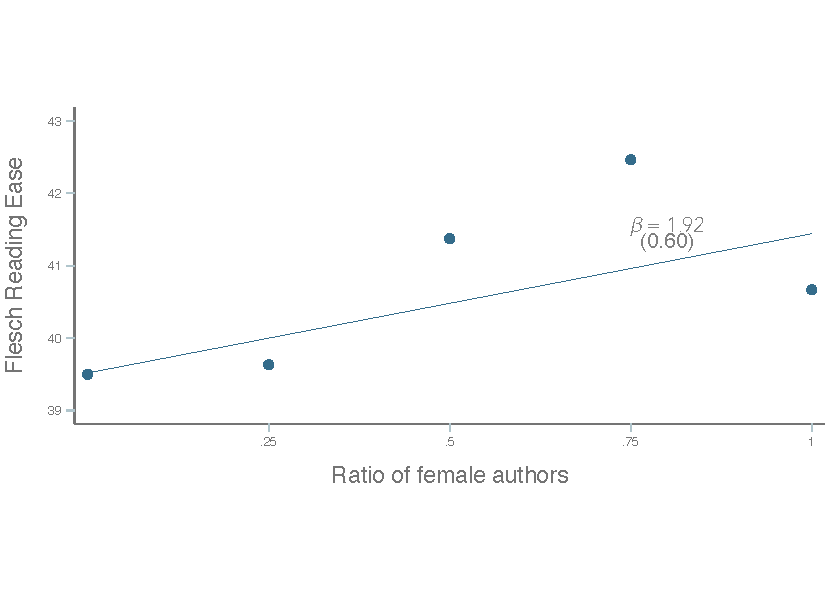
\includegraphics[width=12.3cm,trim=0cm 2cm 0cm 1.9cm,clip]{0-images/generated/Figure-1.pdf}
		\floatfoot{\tiny\textit{Notes}. Sample 9,117 articles. Figure plots abstract readability against the ratio of female authors on a paper.}
	}
\end{figure}

Instead, I assume an article's gender is related to its proportion of female authors. A gender readability gap---if it exists---is presumably a function of (i) the probability a passage of text was written and\slash or revised by a female co-author; and (ii) referees' beliefs about female authors' contributions to the writing and\slash or revision of a co-authored paper. Prior research suggests co-authors---regardless of seniority---share responsibility for writing and (especially) revising collaborative work~\citep[see, \emph{e.g.}, ][]{Hart2000a,Kumar2016}. Thus, the intersection of (i) and (ii) is likely positively related to the ratio of female authors on a paper.

\autoref{figureX} corroborates this hypothesis. It plots abstract readability against a paper's ratio of female authors. The slope of the regression line is positive, relatively large (1.88 points on the Flesch Reading Ease scale) and statistically significant; however the relationship is not entirely linear. In particular, it appears to be close to zero when women make up fewer than 50 percent of authors and increasing in the share of female authors only after that. For this reason, I define papers with a strict minority of female authors as male-authored; for papers with 50 percent or more female authors, I allow an article's gender to increase linearly with its proportion of female authors. For robustness, however, I also repeat most analyses (a) on the sample of solo-authored papers, only; (b) comparing papers with a senior female co-author to entirely male-authored papers; (c) on the subset of papers authored by a single gender; (d) using a binary variable equal to one if at least one author is female; and (e) using a binary variable equal to one if at least half of all authors are female. Standard errors from (a) and (c) tend to be larger; those from (b), (d) and (e) usually similarly sized or smaller. In general, however, results do not meaningfully change (\aref{appendixalternativemeasure}).

\section{Stylised facts}
\label{stylisedfacts}

\subsection{Women are under-represented in top-four economics journals}
\label{underrepresentation}

\begin{figure}
	\floatbox{figure}[\FBwidth]
	{
		\caption{The representation of women in top economics journals}\label{figure5}
	}
	{
	\begin{minipage}{0.3\textwidth}
		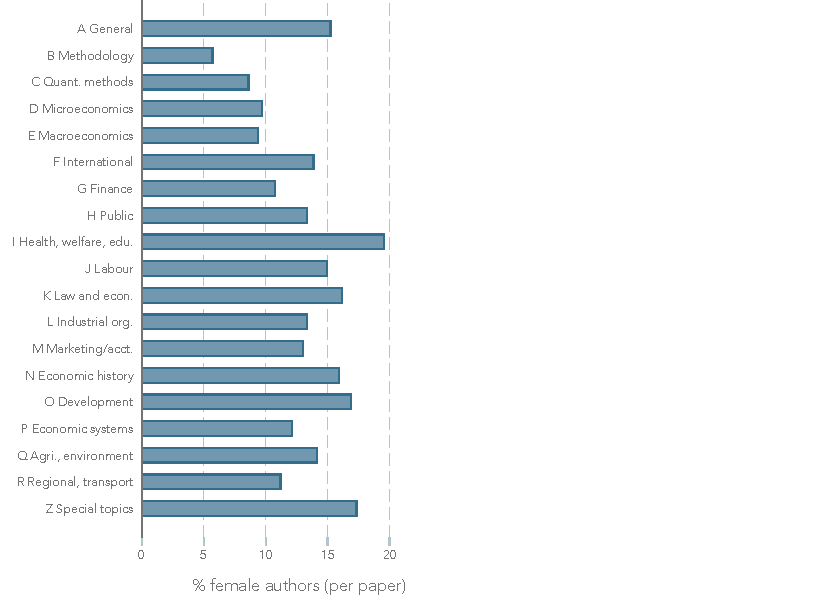
\includegraphics[trim=0.25cm 0cm 6.7cm 0cm, clip, width=1.1\linewidth]{0-images/generated/Figure-2-jel.pdf}
	\end{minipage}
	\begin{minipage}{0.65\textwidth}
		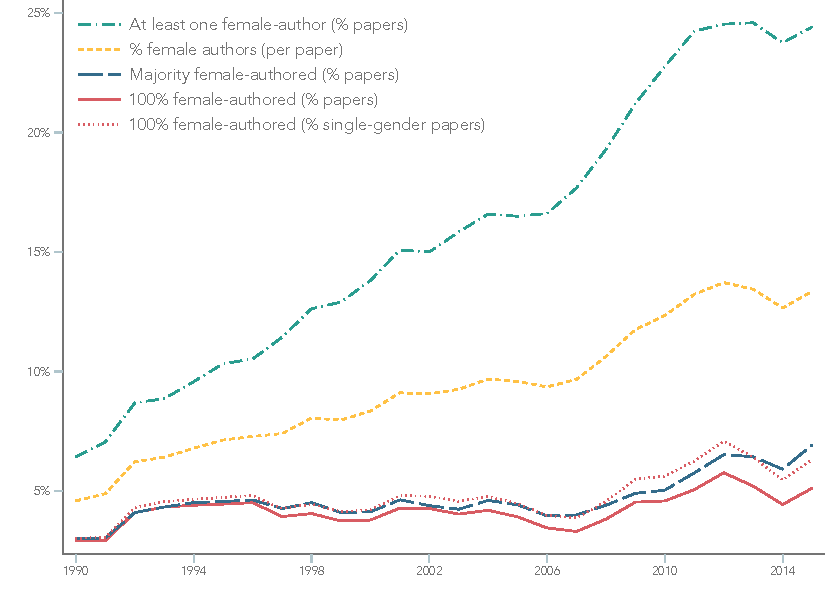
\includegraphics[width=0.95\linewidth]{0-images/generated/Figure-2-time.pdf}
	\end{minipage}
		\floatfoot{\tiny \textit{Notes}. Sample 5,211 articles. Graphs illustrate the representation of female authors in articles published in top-four economics journals. Figure on the left is the average share of female authors per paper broken down by primary \textit{JEL} category; figure on the right displays the evolution of papers' gender composition over time as five-year moving averages.}
	}
\end{figure}

The right-hand graph in \autoref{figure5} illustrates women's representation in top-four economics journals over time. The number of papers these journals publish with at least one female author has been steadily increasing over the past several decades---from about 5 percent in the late 1980s to around 25 percent in 2015. Growth in the average share of female authors per paper, however, is more muted: it was about 3--4 percent in the late 1980s; by 2015 it had only increased to 15 percent. The discrepancy between these two figures is because growth in female authorship is largely thanks to an increase in the number of mixed-gendered papers authored by a strict minority of women. In fact, there has been almost no growth in the percentage of papers that are either majority or exclusively female-authored: both figures have hovered around 4--5 percent since the early 1990s. \emph{Econometrica} publishes the fewest exclusively female-authored papers (3 percent of all papers published since 1990), \emph{AER} the most (6 percent); \emph{JPE} and \emph{QJE} fall in between (4 and 5 percent, respectively). Percentages are only slightly higher (and rankings identical) for papers with a strict majority of female authors.

The left-hand graph in \autoref{figure5} plots the average percentage of female authors per paper across primary \emph{JEL} categories for articles published between 1990--2015. There are clear differences across fields. The average percentage of female authors per paper was lowest in \emph{JEL} codes B (history of economic thought, methodology and heterodox approaches), C (mathematical and quantitative methods), D (microeconomics) and E (macroeconomics and monetary economics) and highest in I (health, education and welfare), Z (other special topics) and O (economic development, innovation, technological change, and growth). Despite this variation, the percentage of female authors per paper does not exceed 20 percent in any field.

\subsection{Women's papers are more readable}
\label{articlelevel}

\autoref{table2} compares textual characteristics between male-authored papers (defined as having a ratio of female authors below 50 percent) and female-authored papers (defined as having a ratio of female authors at or above 50 percent). It suggests women write shorter, simpler sentences: they contain fewer characters, fewer syllables, fewer words and fewer ``hard'' words. Differences are highly statistically significant.

\begin{table}
    \footnotesize
    \centering
    \begin{threeparttable}
        \caption{Textual characteristics per sentence by gender}
        \label{table2}
        \begin{tabular}{p{4cm}S@{}S@{}S@{}}
            \toprule
            &{Men}&{Women}&{Difference}\\
            \midrule
            \mrow{4cm}{No. characters}    &      134.72&      131.39&       -3.32** \\
                                          &      (0.42)&      (1.30)&      (1.37)   \\
            \mrow{4cm}{No. words}         &       24.15&       23.39&       -0.76***\\
                                          &      (0.08)&      (0.24)&      (0.25)   \\
            \mrow{4cm}{No. syllables}     &       40.64&       39.15&       -1.48***\\
                                          &      (0.13)&      (0.40)&      (0.42)   \\
            \mrow{4cm}{No. polysyllabic words}&        4.69&        4.40&       -0.29***\\
                                          &      (0.02)&      (0.06)&      (0.06)   \\
            \mrow{4cm}{No. difficult words}&        9.38&        9.03&       -0.35***\\
                                          &      (0.03)&      (0.10)&      (0.11)   \\
            \midrule
            No. observations              &       8,266&         851&       9,117   \\
            \bottomrule
        \end{tabular}
        \begin{tablenotes}
            \tiny
            \item \textit{Notes}. Figures are means of textual characteristics (per sentence) by sex. Male-authored papers are defined as having a ratio of female authors below 50 percent; female-authored papers are those with a ratio of female authors at or above 50 percent. Last column subtracts male means from female means. Standard errors in parentheses. ***, ** and * difference statistically significant at 1\%, 5\% and 10\%, respectively.
        \end{tablenotes}
    \end{threeparttable}
\end{table}

\autoref{table3_FemRatio} presents results from 45 separate ordinary least squares (OLS) regressions of readability scores on the ratio of female authors (papers with fewer than 50 percent female authors are classified as male, see \autoref{gender}). Column (1) includes journal and editor fixed effects and controls for blind review and its interaction with the ratio of female authors on a paper. Columns (2) and (3) add journal-year interaction dummies.\footnote{The coefficients on the journal dummies in (2) are presented in \aref{appendixarticlelevel}. Compared to \emph{AER}, all five scores agree that \emph{Econometrica} is harder to read; four out of five scores suggest \emph{JPE} is, too, while \emph{QJE} is easier.} Column (4) introduces controls for paper $j$'s number of co-authors ($N_j$) and the dynamic institution effects described in \aref{appendixcontrols}. Column (5) adds a dummy variable capturing English fluency; it also controls for article quality (citations (asinh)), co-author prominence ($\text{max. }T$) and seniority at the time of publication ($\text{max. }t$). Columns (6)--(9) are estimated on the sample of articles published after 1990. (7) includes fixed effects for primary \emph{JEL} categories. (8) replaces it with three binary variables meant to capture how theoretical vs. empirical a paper is. (9) includes fixed effects for tertiary \emph{JEL} categories.\footnote{\label{FootnoteAERpp}Due to small sample sizes, column (9) includes 563 articles from \emph{AER P\&P}, coded as a separate journal. Papers published in \emph{AER P\&P} are selected and edited by the American Economic Association's president-elect with the help of a Program Committee (see \href{https://www.aeaweb.org/journals/pandp/about-pandp}{www.aeaweb.org} for more details). \emph{P\&P} does not publish abstracts in its print version; only select years (2003 and 2011--2015) and papers were available online when I collected the data. Excluding these articles does not impact results or conclusions: coefficients are similar to those in column (9), but standard errors are somewhat higher.}

Results in \autoref{table3_FemRatio} suggest that abstracts written by women score about 1--2 points higher on the Flesch Reading Ease scale; according to the four grade-level measures, they take about 1--5 fewer months of schooling to understand. Percentage-wise, women write about 1--4 percent better than men.

\begin{table}
    \footnotesize
    \centering
    \begin{threeparttable}
        \caption{Gender differences in readability, article-level analysis}
        \label{table3_FemRatio}
        \begin{tabular}{p{2cm}S@{}S@{}S@{}S@{}S@{}S@{}S@{}S@{}S@{}}
            \toprule
            &\multicolumn{5}{c}{1950--2015}&\multicolumn{4}{c}{1990--2015}\\\cmidrule(lr){2-6}\cmidrule(lr){7-10}&{(1)}&{(2)}&{(3)}&{(4)}&{(5)}&{(6)}&{(7)}&{(8)}&{(9)}\\
            \midrule
            \mrow{3cm}{Flesch}            &        1.25** &        1.23** &        1.23** &        1.26** &        1.49***&        1.31** &        1.36** &        1.29** &        1.97** \\
                                          &      (0.53)   &      (0.52)   &      (0.53)   &      (0.54)   &      (0.56)   &      (0.59)   &      (0.54)   &      (0.60)   &      (0.77)   \\
            \mrow{3cm}{Flesch-Kincaid}    &        0.23*  &        0.22*  &        0.23*  &        0.24*  &        0.26*  &        0.34** &        0.37***&        0.34** &        0.46***\\
                                          &      (0.13)   &      (0.13)   &      (0.13)   &      (0.13)   &      (0.14)   &      (0.15)   &      (0.14)   &      (0.15)   &      (0.17)   \\
            \mrow{3cm}{Gunning Fog}       &        0.36** &        0.36** &        0.37** &        0.40** &        0.42***&        0.51***&        0.50***&        0.51***&        0.61***\\
                                          &      (0.15)   &      (0.15)   &      (0.15)   &      (0.15)   &      (0.16)   &      (0.18)   &      (0.15)   &      (0.18)   &      (0.19)   \\
            \mrow{3cm}{SMOG}              &        0.25** &        0.25** &        0.26** &        0.27** &        0.29** &        0.32** &        0.31***&        0.33** &        0.40***\\
                                          &      (0.10)   &      (0.10)   &      (0.10)   &      (0.11)   &      (0.11)   &      (0.12)   &      (0.11)   &      (0.13)   &      (0.14)   \\
            \mrow{3cm}{Dale-Chall}        &        0.08   &        0.08   &        0.08   &        0.08   &        0.09   &        0.11*  &        0.11*  &        0.11*  &        0.17** \\
                                          &      (0.05)   &      (0.05)   &      (0.05)   &      (0.05)   &      (0.05)   &      (0.06)   &      (0.06)   &      (0.06)   &      (0.07)   \\
            \midrule
            No. obs.                      &       9,117   &       9,117   &       9,117   &       9,117   &       9,117   &       5,211   &       5,211   &       5,211   &       5,774   \\
            \midrule
            Editor               &           {\ding{51}}   &           {\ding{51}}   &           {\ding{51}}   &           {\ding{51}}   &           {\ding{51}}   &           {\ding{51}}   &           {\ding{51}}   &           {\ding{51}}   &           {\ding{51}}   \\
            Blind                         &           {\ding{51}}   &           {\ding{51}}   &           {\ding{51}}   &           {\ding{51}}   &           {\ding{51}}   &           {\ding{51}}   &           {\ding{51}}   &           {\ding{51}}   &           {\ding{51}}   \\
            Journal                       &           {\ding{51}}   &           {\ding{51}}   &               &               &               &               &               &               &               \\
            Year                          &               &           {\ding{51}}   &               &               &               &               &               &               &               \\
            Journal\(\times\)Year                  &               &               &           {\ding{51}}   &           {\ding{51}}   &           {\ding{51}}   &           {\ding{51}}   &           {\ding{51}}   &           {\ding{51}}   &           {\ding{51}}   \\
            \(N_j\)                       &               &               &               &           {\ding{51}}   &           {\ding{51}}   &           {\ding{51}}   &           {\ding{51}}   &           {\ding{51}}   &           {\ding{51}}   \\
            Institution                   &               &               &               &           {\ding{51}}   &           {\ding{51}}   &           {\ding{51}}   &           {\ding{51}}   &           {\ding{51}}   &           {\ding{51}}   \\
            Quality                       &               &               &               &               &          {\(\text{\ding{51}}^1\)}   &          {\(\text{\ding{51}}^1\)}   &          {\(\text{\ding{51}}^1\)}   &          {\(\text{\ding{51}}^1\)}   &          {\(\text{\ding{51}}^1\)}   \\
            Native speaker                &               &               &               &               &           {\ding{51}}   &           {\ding{51}}   &           {\ding{51}}   &           {\ding{51}}   &           {\ding{51}}   \\
            \textit{JEL} (primary)        &               &               &               &               &               &               &           {\ding{51}}   &               &               \\
            Theory/empirical              &               &               &               &               &               &               &               &           {\ding{51}}   &               \\
            \textit{JEL} (tertiary)       &               &               &               &               &               &               &               &               &           {\ding{51}}   \\
            \bottomrule
        \end{tabular}
        \begin{tablenotes}
            \tiny
            \item \textit{Notes}. Figures represent coefficients on female ratio from 45 separate OLS regressions of readability scores on the ratio of female authors (papers with fewer than 50 percent female authors are classified as male, see~\autoref{gender}). (6)--(9) are estimated on the sample of papers published on or after 1990 with a primary \textit{JEL} code; (9) includes 563 articles from \textit{AER P\& P} (see~\autoref{FootnoteAERpp}). Quality controls denoted by \(\text{\ding{51}}^1\) include citation count (asinh), \(\text{max. }T\) fixed effects (author prominence) and \(\text{max. }t\) (author seniority). Standard errors clustered on editor in parentheses. ***, ** and * statistically significant at 1\%, 5\% and 10\%, respectively.
        \end{tablenotes}
    \end{threeparttable}
\end{table}

\aref{appendixjel} explores field in more detail; \aref{appendixauthorlevel} analyses readability at the author-level. Conditional on other explanatory variables, I find little evidence that field drives results in \autoref{table3_FemRatio}. After accounting for author-specific heterogeneity, the gender gap in readability rises to 2--6 percent.

\subsection{Women's papers improve more during peer review}
\label{nber}

\subsubsection{Estimation strategy}
\label{nberidentification}

In this section, I analyse readability changes that occurred during peer review by comparing abstracts pre- and post-review. My first estimation strategy simply regresses each paper's change in score on its gender composition. To understand it, note that the readability of a published paper depends on its earlier draft readability as well as factors that affect writing clarity any time after it was initially drafted:\begin{equation}\label{equation2}
	R_{jP}=R_{jW}+\beta_{0P}+\beta_{1P}\,\text{female ratio}_j+\bm\uptheta_P\,\vect X_{jP}+\mu_{jP}+\vep_{jP},
\end{equation}where $R_{jP}$ and $R_{jW}$ are readability scores for working ($W$) and published ($P$) versions of paper $j$, respectively. $\beta_{1P}$ is the coefficient of interest and reflects the particular impact $\text{female ratio}_j$ has in peer review. $\vect X_{jP}$ and $\mu_{jP}$ are $P$-specific observable and unobservable components, respectively. $\vep_{jP}$ is $P$'s error term.

Correlation between $R_{jW}$ and $\text{female ratio}_j$ may bias OLS estimates of $\beta_{1P}$. \autoref{equation3} eliminates the distortion by subtracting $R_{jW}$ from both sides of \autoref{equation2}:\begin{equation}\label{equation2}
	R_{jP}=R_{jW}+\beta_{0P}+\beta_{1P}\,\text{female ratio}_j+\bm\uptheta_P\,\vect X_{jP}+\mu_{jP}+\vep_{jP},
\end{equation}Assuming zero partial correlation between $\text{female ratio}_j$ and $\mu_{jP}$, OLS generates an unbiased estimate of $\beta_{1P}$.\footnote{\label{FootnoteColliders}Note that zero correlation between $\text{female ratio}_j$ and $\mu_{jP}$ does not preclude biased estimates of $\beta_{1P}$ when $\mu_{jP}$ is correlated with other explanatory variables that are, in turn, correlated with $\text{female ratio}_j$ by some factor independent of $\mu_{jP}$. Unbiasedness instead requires zero \emph{partial} correlation between $\mu_{jP}$ and $\text{female ratio}_j$.}

An alternative strategy based on \citet{Ashenfelter1994} separately estimates gender differences in the draft and final versions of papers using generalised least squares (GLS). The contemporaneous effect of peer review is identified post-estimation by subtracting coefficients. To implement this set-up, I combine \autoref{equation2} with: (i) the relationship between readability scores and the gender composition of a paper before peer review; and (ii) an equation accounting for potential correlation between observable controls and version-invariant unobservables. The former is defined as:\begin{equation}\label{equation3}
	R_{jP}-R_{jW}=\,\beta_{0P}+\beta_{1P}\,\text{female ratio}_j+\bm\uptheta_P\,\vect X_{jP}+\mu_{jP}+\vep_{jP}.
\end{equation}where $\beta_{1W}$ reflects $\text{female ratio}_j$'s impact on readability prior to peer review; $\vect X_{jW}$ and $\mu_{jW}$ are version-invariant observable and unobservable components, respectively; $\vep_{jW}$ is version $W$'s error term. \autoref{equation5} then defines a general structure for potential correlation between $\mu_{jW}$ and observable variables in both \autoref{equation4} and \autoref{equation2}:\begin{equation}\label{equation5}
\mu_{jW}=\gamma+\eta\,\text{female ratio}_j+\bm\updelta_W\,\vect X_{jW}+\bm\updelta_P\,\vect X_{jP}+\omega_j,
\end{equation}where $\omega_j$ is uncorrelated with $\text{female ratio}_j$, $\vect X_{jW}$ and $\vect X_{jP}$. Substituting \autoref{equation5} into \autoref{equation4} generates the following reduced form representation of $R_{jW}$:\begin{equation}\label{equation5}
\mu_{jW}=\gamma+\eta\,\text{female ratio}_j+\bm\updelta_W\,\vect X_{jW}+\bm\updelta_P\,\vect X_{jP}+\omega_j,
\end{equation}where $\wt\beta_{0W}=\beta_{0W}+\gamma$, $\wt\beta_{1W}=\beta_{1W}+\eta$, $\wt{\bm\uptheta}_W=\bm\uptheta_W+\bm\updelta_W$ and $\wt\vep_{jW}=\vep_{jW}+\omega_j$. $R_{jP}$'s reduced form is similarly found by substituting \autoref{equation6} into \autoref{equation2}:\begin{equation}\label{equation7}
	R_{jP}=\,(\wt\beta_{0W}+\beta_{0P})+(\wt\beta_{1W}+\beta_{1P})\,\text{female ratio}_j+\wt{\bm\uptheta}_W\,\vect X_{jW}+\wt{\bm\uptheta}_P\,\vect X_{jP}+\mu_{jP}+\wt\vep_{jP},
\end{equation}where $\wt{\bm\uptheta}_P=\bm\uptheta_P+\bm\updelta_P$ and $\wt\vep_{jP}=\wt\vep_{jW}+\vep_{jP}$. \autoref{equation6} and \autoref{equation7} are explicitly estimated via feasible GLS (FGLS). $\beta_{1P}$ is identified post-estimation by subtracting reduced form coefficients. Assuming zero partial correlation between $\mu_{jP}$ and $\text{female ratio}_j$, it also generates an unbiased estimate of $\beta_{1P}$.

\subsubsection{Results}
\label{nberresults}

\begin{table}
    \footnotesize
    \centering
    \begin{threeparttable}
        \caption{Textual characteristics, published papers vs. drafts}
        \label{table5}
        \sisetup{group-digits=false}
        \begin{tabular}{p{4cm}S@{}S@{}S[round-precision=3]S@{}S@{}S[round-precision=3]S[round-precision=3]}
            \toprule
            &\multicolumn{3}{c}{{Men}}&\multicolumn{3}{c}{{Women}}&\\\cmidrule(lr){2-4}\cmidrule(lr){5-7}&{\crcell[b]{Working\\[-0.1cm]paper}}&{\crcell[b]{Published\\[-0.1cm]article}}&{Difference}&{\crcell[b]{Working\\[-0.1cm]paper}}&{\crcell[b]{Published\\[-0.1cm]article}}&{Difference}&{\crcell[b]{Diff.-in\\[-0.1cm]diff.}}\\
            \midrule
            \mrow{3cm}{No. sentences}     &        6.47&        5.10&      -1.375***&        6.77&        5.06&      -1.711***&      -0.337** \\
                                          &      (0.06)&      (0.04)&     (0.054)   &      (0.15)&      (0.08)&     (0.139)   &     (0.149)   \\
            \mrow{3cm}{No. characters}    &      862.39&      649.77&    -212.612***&      907.27&      636.03&    -271.245***&     -58.564***\\
                                          &      (7.19)&      (4.67)&     (7.161)   &     (18.52)&     (10.32)&    (18.440)   &    (19.599)   \\
            \mrow{3cm}{No. words}         &      155.59&      115.70&     -39.889***&      164.28&      113.60&     -50.674***&     -10.747***\\
                                          &      (1.32)&      (0.85)&     (1.323)   &      (3.41)&      (1.91)&     (3.424)   &     (3.630)   \\
            \mrow{3cm}{No. syllables}     &      256.98&      193.34&     -63.640***&      268.90&      187.73&     -81.172***&     -17.496***\\
                                          &      (2.15)&      (1.40)&     (2.135)   &      (5.54)&      (3.08)&     (5.503)   &     (5.842)   \\
            \mrow{3cm}{No. polysyllabic words}&       28.39&       21.80&      -6.590***&       28.96&       20.62&      -8.341***&      -1.738***\\
                                          &      (0.28)&      (0.18)&     (0.245)   &      (0.71)&      (0.41)&     (0.627)   &     (0.668)   \\
            \mrow{3cm}{No. difficult words}&       58.44&       44.64&     -13.798***&       60.24&       42.40&     -17.839***&      -4.034***\\
                                          &      (0.51)&      (0.33)&     (0.482)   &      (1.30)&      (0.74)&     (1.199)   &     (1.313)   \\
            \midrule
            \mrow{3cm}{Flesch}            &       41.40&       41.15&      -0.249   &       42.48&       43.10&       0.613   &       0.831*  \\
                                          &      (0.26)&      (0.18)&     (0.185)   &      (0.66)&      (0.42)&     (0.449)   &     (0.499)   \\
            \mrow{3cm}{Flesch-Kincaid}    &      -13.63&      -13.38&       0.251***&      -13.53&      -13.00&       0.535***&       0.278** \\
                                          &      (0.06)&      (0.05)&     (0.049)   &      (0.15)&      (0.11)&     (0.122)   &     (0.134)   \\
            \mrow{3cm}{Gunning Fog}       &      -17.28&      -17.03&       0.253***&      -17.13&      -16.58&       0.553***&       0.290*  \\
                                          &      (0.07)&      (0.05)&     (0.055)   &      (0.18)&      (0.13)&     (0.140)   &     (0.149)   \\
            \mrow{3cm}{SMOG}              &      -15.14&      -15.00&       0.144***&      -15.03&      -14.69&       0.333***&       0.185*  \\
                                          &      (0.05)&      (0.03)&     (0.035)   &      (0.13)&      (0.09)&     (0.094)   &     (0.097)   \\
            \mrow{3cm}{Dale-Chall}        &      -10.84&      -10.93&      -0.090***&      -10.70&      -10.71&      -0.005   &       0.085** \\
                                          &      (0.02)&      (0.02)&     (0.015)   &      (0.06)&      (0.04)&     (0.037)   &     (0.042)   \\
            \midrule
            No. observations              &       1,715&       1,715&       1,715   &         273&         273&         273   &       1,988   \\
            \bottomrule
        \end{tabular}
        \begin{tablenotes}
            \tiny
            \item \textit{Notes}. Figures are means of textual characteristics by sex for NBER working papers and published articles. Male-authored papers are defined as having a ratio of female authors below 50 percent; female-authored papers are those with a ratio of female authors at or above 50 percent. Penultimate columns in each panel subtract working paper figures from published article figures for men (first panel) and women (second panel); difference-in-differences (female less male) shown in the final column. Standard errors in parentheses. ***, ** and * difference statistically significant at 1\%, 5\% and 10\%, respectively.
        \end{tablenotes}
    \end{threeparttable}
\end{table}

\autoref{table5} compares textual characteristics between a paper's draft and final versions in the samples of male-authored (female ratio below 50 percent) and female-authored manuscripts (female ratio at or above 50 percent). It suggests abstract text is altered during peer review. According to the first panel, draft abstracts are longer---more characters, words and sentences---and denser---more syllables, polysyllabic words and difficult words. The biggest changes are made to female-authored papers: figures in column six are 20--30 percent higher (in absolute value) than those in column three. The second panel of \autoref{table5} suggests women's papers become more readable during peer review relative to men's. More generally, they also seem to indicate that peer review improves readability, although results are less clear for male-authored papers.

\autoref{table6_FemRatio}'s first panel displays results from OLS estimation of \autoref{equation2}. Conditional on draft readability, published female-authored papers are more readable than published male-authored papers. Moreover, published article readability positively correlates with draft readability: coefficients on $R_{jW}$ are about 0.8 and consistently highly significant.

\begin{sidewaystable}
    \footnotesize
    \centering
    \begin{threeparttable}
        \caption{The impact of peer review on the gender readability gap}
        \label{table6_FemRatio}
        \begin{tabular}{p{3cm}S@{}S@{}S@{}S@{}S@{}S@{}S@{}S@{}S@{}S@{}S@{}}
            \toprule
            &\multicolumn{3}{c}{{OLS (score)}}&\multicolumn{2}{c}{{OLS ($\Delta$ in score)}}&\multicolumn{6}{c}{{FGLS (score)}}\\\cmidrule(lr){2-4}\cmidrule(lr){5-6}\cmidrule(lr){7-12}&&&&&&\multicolumn{2}{c}{{Working paper}}&\multicolumn{2}{c}{{Published paper}}&\multicolumn{2}{c}{{Difference}}\\\cmidrule(lr){7-8}\cmidrule(lr){9-10}\cmidrule(lr){11-12}&{\(R_{jW}\)}&{\crcell[b]{Female\\[-0.1cm]ratio}}&{\crcell[b]{Blind$\times$\\[-0.1cm]fem. ratio}}&{\crcell[b]{Female\\[-0.1cm]ratio}}&{\crcell[b]{Blind$\times$\\[-0.1cm]fem. ratio}}&{\crcell[b]{Female\\[-0.1cm]ratio}}&{\crcell[b]{Blind$\times$\\[-0.1cm]fem. ratio}}&{\crcell[b]{Female\\[-0.1cm]ratio}}&{\crcell[b]{Blind$\times$\\[-0.1cm]fem. ratio}}&{\crcell[b]{Female\\[-0.1cm]ratio}}&{\crcell[b]{Blind$\times$\\[-0.1cm]fem. ratio}}\\
            \midrule
            Flesch                        &        0.83***&        1.47** &       -2.15   &        1.19*  &       -1.75   &        1.68   &       -2.35   &        2.87***&       -4.10*  &        1.19*  &       -1.75   \\
                                          &      (0.02)   &      (0.62)   &      (3.84)   &      (0.70)   &      (2.18)   &      (1.05)   &      (3.37)   &      (1.08)   &      (2.16)   &      (0.69)   &      (2.14)   \\
            Flesch-Kincaid                &        0.74***&        0.53***&       -0.92   &        0.48** &       -0.74   &        0.18   &       -0.70   &        0.66** &       -1.44***&        0.48** &       -0.74   \\
                                          &      (0.04)   &      (0.21)   &      (0.83)   &      (0.20)   &      (0.52)   &      (0.26)   &      (0.77)   &      (0.27)   &      (0.44)   &      (0.20)   &      (0.51)   \\
            Gunning Fog                   &        0.76***&        0.54** &       -0.93   &        0.48** &       -0.76   &        0.26   &       -0.71   &        0.74***&       -1.47***&        0.48** &       -0.76   \\
                                          &      (0.03)   &      (0.22)   &      (0.80)   &      (0.22)   &      (0.57)   &      (0.28)   &      (0.85)   &      (0.28)   &      (0.53)   &      (0.21)   &      (0.56)   \\
            SMOG                          &        0.79***&        0.31** &       -0.59   &        0.27*  &       -0.48   &        0.20   &       -0.52   &        0.47***&       -1.00** &        0.27** &       -0.48   \\
                                          &      (0.03)   &      (0.15)   &      (0.56)   &      (0.14)   &      (0.39)   &      (0.17)   &      (0.61)   &      (0.18)   &      (0.40)   &      (0.14)   &      (0.39)   \\
            Dale-Chall                    &        0.85***&        0.18***&       -0.20   &        0.14** &       -0.20   &        0.21** &       -0.04   &        0.35***&       -0.24   &        0.14** &       -0.20   \\
                                          &      (0.02)   &      (0.05)   &      (0.20)   &      (0.06)   &      (0.13)   &      (0.10)   &      (0.23)   &      (0.10)   &      (0.20)   &      (0.06)   &      (0.13)   \\
            \midrule
            No. observations              &               &       1,988   &               &       1,988   &               &       1,988   &               &       1,988   &               &       1,988   &               \\
            \midrule
            Editor effects       &               &           {\ding{51}}   &               &           {\ding{51}}   &               &           {\ding{51}}   &               &           {\ding{51}}   &               &               &               \\
            Journal\(\times\)Year effects          &               &           {\ding{51}}   &               &           {\ding{51}}   &               &           {\ding{51}}   &               &           {\ding{51}}   &               &               &               \\
            \(N_j\)                       &               &           {\ding{51}}   &               &           {\ding{51}}   &               &           {\ding{51}}   &               &           {\ding{51}}   &               &               &               \\
            Quality controls              &               &          {\(\text{\ding{51}}^2\)}   &               &          {\(\text{\ding{51}}^2\)}   &               &          {\(\text{\ding{51}}^2\)}   &               &          {\(\text{\ding{51}}^2\)}   &               &               &               \\
            Native speaker                &               &           {\ding{51}}   &               &           {\ding{51}}   &               &           {\ding{51}}   &               &           {\ding{51}}   &               &               &               \\
            Theory/emp. effects           &               &           {\ding{51}}   &               &           {\ding{51}}   &               &           {\ding{51}}   &               &           {\ding{51}}   &               &               &               \\
            \bottomrule
        \end{tabular}
        \begin{tablenotes}
            \tiny
            \item \textit{Notes}. Panel one displays coefficients from estimating~\autoref{equation2} directly via OLS; standard errors clustered by editor in parentheses. Panel two displays coefficients from OLS estimation of~\autoref{equation3}; standard errors clustered by year in parentheses. Panel three displays coefficients from FGLS estimation of \autoref{equation6} and \autoref{equation7}; standard errors clustered by year and robust to cross-model correlation in parentheses. Quality controls denoted by \(\text{\ding{51}}^2\) include citation count (asinh), \(\text{max. }T\) (author prominence) and \(\text{max. }t\) (author seniority). The variable "female ratio" defines papers with a strict minority of female authors as male-authored; for papers with 50 percent or more female authors, it is the ratio of female authors on a paper (see~\autoref{gender} for more details). ***, ** and * statistically significant at 1\%, 5\% and 10\%, respectively.
        \end{tablenotes}
    \end{threeparttable}

\end{sidewaystable}


\autoref{table6_FemRatio}'s remaining columns show results from the two strategies presented in \autoref{nberidentification}. The first strategy regresses each paper's change in score on its ratio of female authors (papers with fewer than 50 percent female authors are classified as male, see \autoref{gender}). As already discussed, an advantage of this strategy is that it more effectively removes the impact of confounding factors---\emph{e.g.}, research field---that are constant between manuscript versions. The FGLS strategy estimates the coefficient on female ratio separately among the sample of working papers and published articles; the impact of gender on the readability gap formed during peer review is the difference between them. The advantage of this strategy is that it allows us to observe an estimate of the gap both before and after peer review.

Results from the first strategy are shown in panel two; results from the second are shown in panel three. Both strategies' estimates of the effect of gender formed during peer review are very similar (columns 4 and 10). They suggest that female-authored abstracts become 2--5 percent more readable while under review. FGLS results further indicate that the gender readability gap is 2--3 times larger in papers' published versions than it was in their pre-print versions.

Interestingly, although citations and abstract readability generally positively correlate with one another (\aref{appendixreadability}), the relationship between citations and the \emph{change} in readability between draft and final versions of a paper is either negative or zero (\aref{appendixdraftcorr}). Although I do not observe how many citations papers would have received had they not gone through peer review, these results tentatively suggest that the revisions women are asked to make during the process may not improve the general quality of their papers as proxied for by citations.

Also included in \autoref{table6_FemRatio} are coefficients on the interaction between female ratio and a dummy variable equal to 1 for papers that underwent double-blind review before the internet. These estimates consistently suggest that the gender readability gap reversed direction when papers were subjected to blind review, although none are statistically significant at traditional levels. In \aref{appendixeventstudy}, I plot average residuals over time for papers published in the \emph{AER} or \emph{QJE} before and after they introduced (or removed) double-blind review from a regression of the differenced readability scores on the ratio of female authors. As the figures illustrates, there is a clear discontinuity in women's average unexplained changes to readability when journals switched to single-blind review (or the internet was introduced). For men, however, unexplained changes do not appear to have been substantially affected by double-blind review, conditional on included controls.

The number of manuscripts---and especially female-authored manuscripts---subjected to double-blind review is small so the coefficients on the interaction between blind review and the ratio of female authors on a paper should be interpreted with caution. Nevertheless, they do provide some (weak) indication that the gender readability gap at least partially results from factors outside of women's control, \emph{e.g.}, editorial and refereeing bias. They may also suggest that masking authors' identities can help reduce peer review's impact on the gender readability gap---but only under certain circumstances. In \aref{appendixdoubleblind}, I analyse the policy's post-internet impact. Gender differences are positive regardless of a journal's official review policy, suggesting that double-blind review may be effective only as long as authors are not identifiable by other means.

\subsubsection{Robustness}
\label{nberrobustness}

In order to conclude that the results presented in the previous section suggest women's papers become more readable while under review, I assume that NBER working papers are not generally released before their authors submit them for peer review.\footnote{Concluding that the gender readability gap is \emph{caused} by peer review requires making the additional assumption that authors do not make post-submission changes to their papers unless requested by referees.} As \aref{appendixtiming} illustrates, this appears to be the case: most manuscripts---and especially most female-authored manuscripts---are submitted to peer review at the same time or before being released as NBER Working Papers.

Another concern is that gender differences in how authors conform to abstract word limits may bias results in \autoref{table6_FemRatio}. To investigate this possibility, I exclude the 642 observations---about 40 percent of the sample---with NBER abstracts longer than the official word limit of the journals in which they were eventually published. Results are presented in \aref{appendixwordlimits}. Coefficient magnitudes are similar to those in \autoref{table6_FemRatio}; standard errors are somewhat larger.

Finally, in an effort to maximise sample sizes, I do not control for field. Although estimates in the second panel arguably implicitly account for field already, I additionally replicate \autoref{table6_FemRatio} with fixed effects for primary \emph{JEL} categories. Results are shown in \aref{appendixnberfield}. Adding \emph{JEL} fixed effects slightly increases standard errors; they otherwise make little difference.

\subsection{Women's papers spend longer under review}
\label{duration}

\begin{quote}

``Writing simply and directly only looks easy''~\citep[][p. 53]{Kimble1994}.
\end{quote}

Good writing takes time~\citep{Hartvigsen1981,Kroll1990}: skilled writers spend longer contemplating a writing assignment, brainstorming and editing; they also write fewer words per minute and produce more drafts~\citep{Faigley1981,Stallard1974}. As a consequence, higher writing standards---and, indeed, higher standards applied more generally~\citep[see, \emph{e.g.},][]{Card2020,Moon2020}---should result in female authors spending longer in peer review, all things equal.

On the other hand, better writing by female economists could perfectly offset some other advantage present in men's papers, conditional on quality. In this case, the time-cost of publishing a paper will instead be gender neutral---since if it weren't, women could reduce their time spent in review by adopting a strategy marginally closer to men's (or visa versa).

To formalise this idea, consider male and female researchers who use strategies $x_m,x_f\in\mathcal X$ to produce papers of identical quality $Q\in\mathcal Q$. Let $q$ represent the function mapping $\mathcal X$ onto $\mathcal Q$ and define $q^{-1}(Q)$ as the set of strategies in $\mathcal X$ that achieve the same $Q$.

If men and women are held to identical standards in peer review, then both will accrue identical rewards, conditional on $Q$, \emph{i.e.},\begin{equation}\label{equation7}
	\begin{split}
		R_{jP}=&\,(\wt\beta_{0W}+\beta_{0P})+(\wt\beta_{1W}+\beta_{1P})\,\text{female ratio}_j\\
		&+\wt{\bm\uptheta}_W\,\vect X_{jW}+\wt{\bm\uptheta}_P\,\vect X_{jP}+\mu_{jP}+\wt\vep_{jP},
	\end{split}
\end{equation}where $x$ is any strategy in $q^{-1}(Q)$ and $a_g(x_g,Q)$ is the acceptance rate for gender $g\in{m,f}$ given strategy $x_g$ and quality $Q$.\footnote{Higher standards come from accepting male-authored papers more often than female-authored papers, conditional on $Q$---\emph{i.e.}, $a_m(x,Q)>a_f(x,Q)$---rewarding men's strategies more than women's strategies even though they both generate identical $Q$---\emph{i.e.}, $a(x_m,Q)>a(x_f,Q)$---or both.}

If men and women are also equally capable researchers, then neither side should have to exert more effort, conditional on acceptance rate (and, hence, $Q$)---\emph{i.e.}, given \autoref{reward}, there must exist some $\hat x_m,\hat x_f\in q^{-1}(Q)$ such that\begin{equation}\label{cost}
	c_m(\hat x_m)=c_f(\hat x_f),
\end{equation}where $c_g(x_g)$ is the cost to gender $g$ of implementing the strategy $x_g$. In the absence of higher standards, \autoref{cost} implies that men's and women's time-cost of review should be equal, conditional on $Q$.

Men's and women's time-cost of review does not appear to be equal. \autoref{figure10} displays histograms of time (in months) between dates male- (defined as having a ratio of female authors below 50 percent) and female-authored papers (defined as having a ratio of female authors above 50 percent) are first submitted to and their final revisions received by the editorial offices of \emph{Econometria} and \emph{REStud}. Women's review times disproportionately cluster above the mean: their articles are five times more likely to experience delays above the 75th percentile than they are to enjoy speedy revisions below the 25th.

\begin{figure}
	
	\floatbox{figure}[\FBwidth]
	{
		\caption{Distribution of review times at \textit{Econometrica} and \textit{REStud}}\label{figure10}
	}
	{
		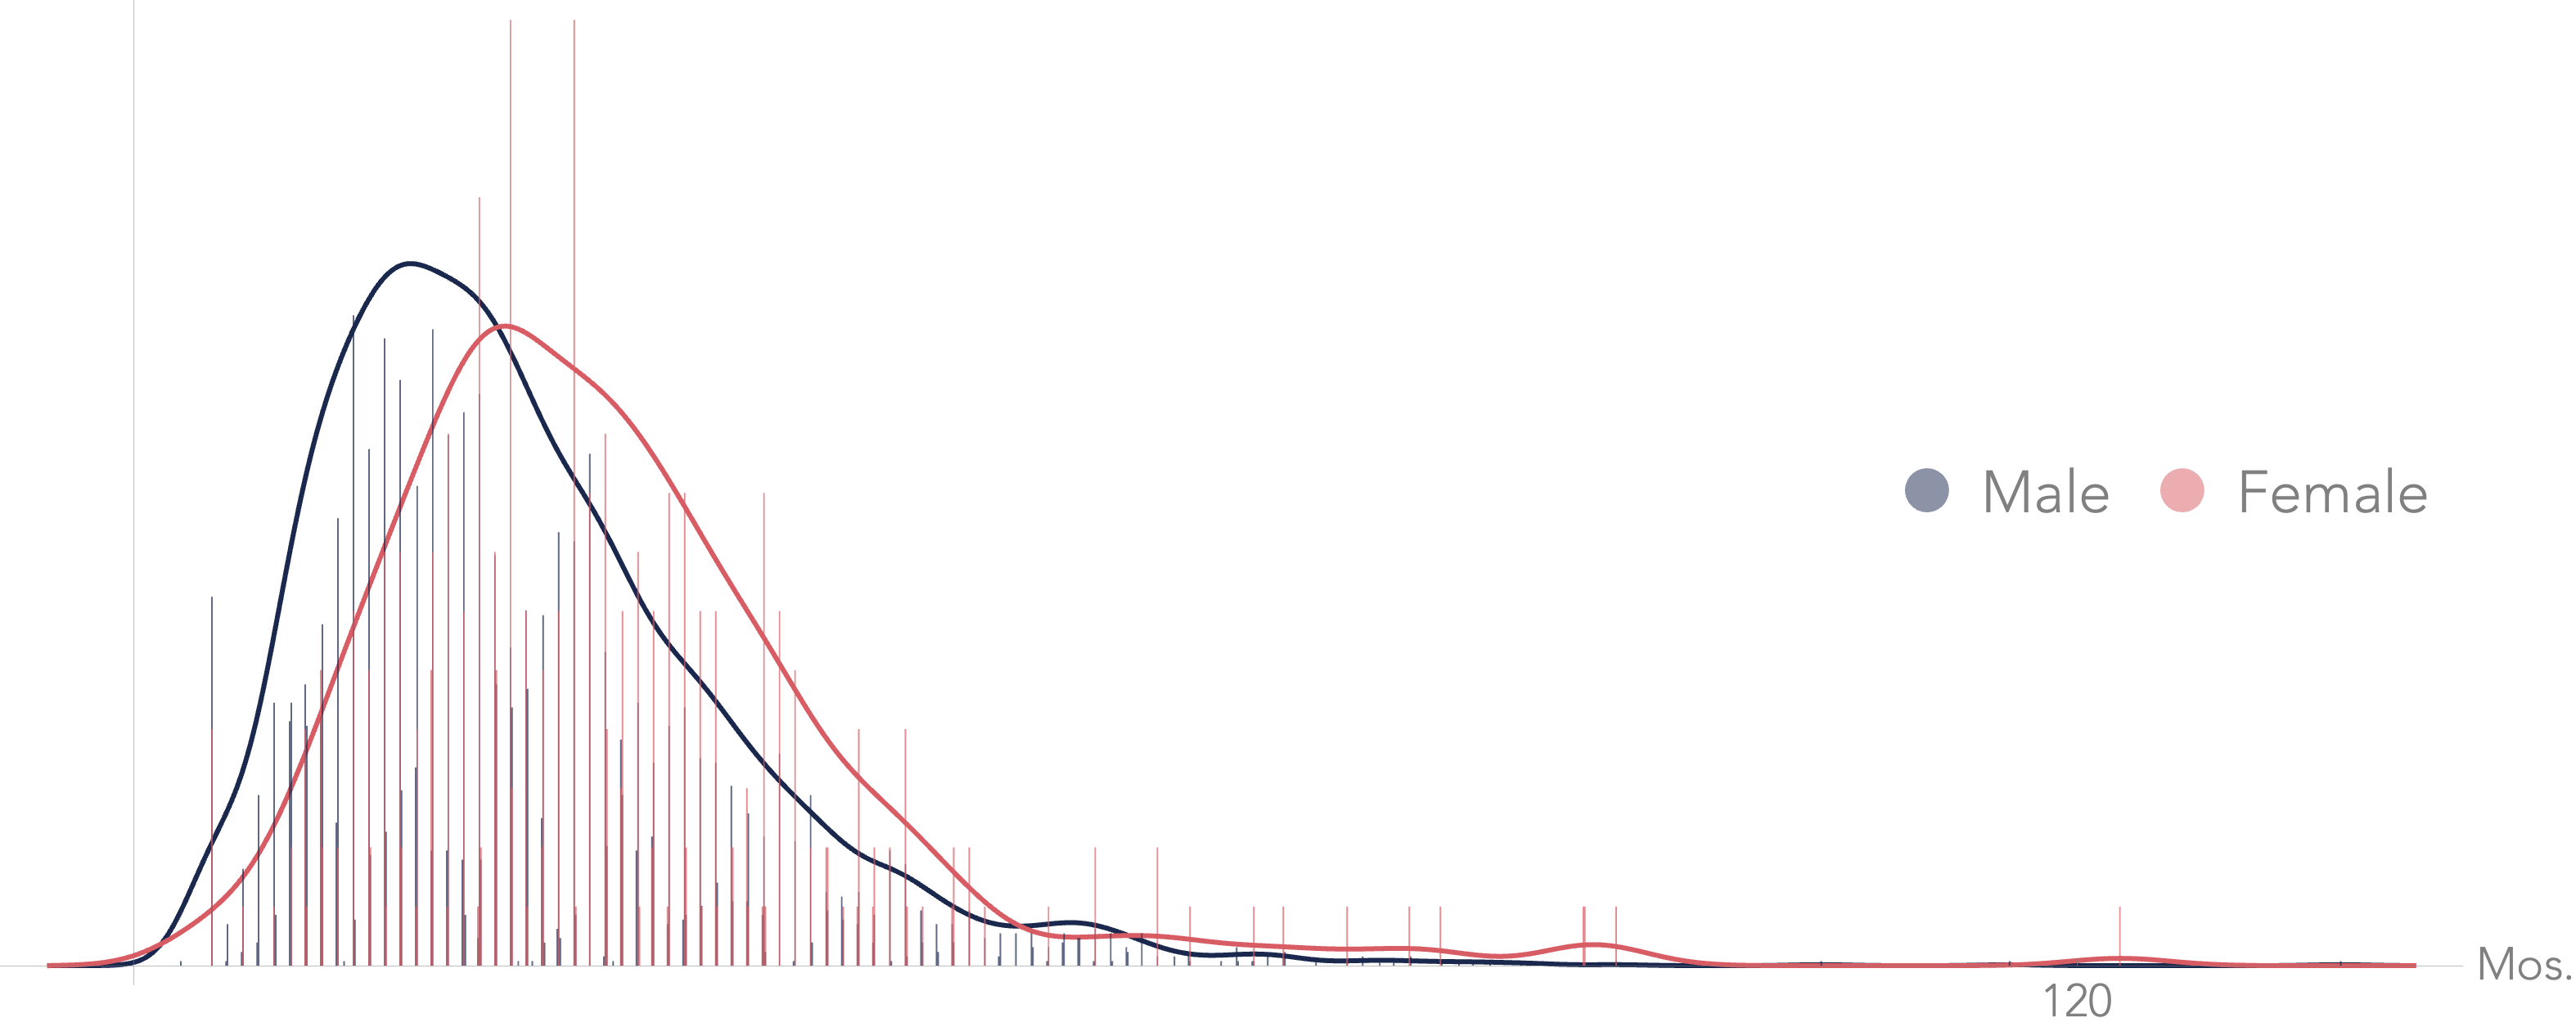
\includegraphics[width=\linewidth]{0-images/generated/Figure-3.png}
		\floatfoot{\tiny \textit{Notes}. Sample 4,435 articles. Histograms of time spent under review for papers published in \textit{Econometrica} and \textit{REStud}. Male-authored papers are defined as having a ratio of female authors below 50 percent; female-authored papers are those with a ratio of female authors at or above 50 percent.}
	}
\end{figure}

\subsubsection{Estimation strategy and results}
\label{durationresults}

For more precision on gender differences in the time-cost of review---and in order to condition explicitly on quality---I build on a model by  \citet{Ellison2002a}:\begin{equation}\label{equation16}
\begin{split}
	\text{revision duration}_j = 	&\, \beta_0+\beta_1\,\text{female ratio}_j +\beta_2\,\text{mother}_j + \beta_3\,\text{birth}_j \\
									& + \beta_4\,\max~t_j + \beta_5\,\text{no. pages}_j + \beta_6\,N_j + \beta_7\,\text{order}_j \\
									& + \beta_8\,\text{citations}_j + \beta_9\,\text{flesch}_j + \beta_{10}\,\text{theory}_j + \beta_{11}\,\text{empirical}_j\\
									& + \beta_{12}\,\text{other}_j + \bm\uptheta\,\vect X_j + \vep_j,
\end{split}
\end{equation}where $\text{female ratio}_j$ is the ratio of female authors on paper $j$ (papers with fewer than 50 percent female authors are classified as male, see \autoref{gender}), $\text{mother}_j$ and $\text{birth}_j$ are binary variables equal to 1 if article $j$'s authors were all mothers to children younger than five and gave birth, respectively, at some point during peer review, $\max.~t_j$ is the number of prior papers published in a top-five economics journal by article $j$'s most prolific co-author, $\text{no. pages}_j$ refers to the page length of the published article, $\text{order}_j$ is the order in which article $j$ appeared in an issue, $\text{citations}_j$ are the asinh-transformed number of subsequent papers citing $j$, $\text{flesch}_j$ is its Flesch Reading Ease score, the dummy variables $\text{theory}_j$, $\text{empirical}_j$ and $\text{other}_j$ account for how theoretical vs. empirical a paper is, and $\vect X_j$ captures additional fixed effects.

I first estimate \autoref{equation16} on data from \emph{Econometrica}. I then re-estimate it excluding readability, motherhood and childbirth controls---which I do not have for papers published in \emph{REStud}---on the entire sample and each journal separately.

\begin{table}
    \begin{adjustwidth}{-0.085cm}{}
    \footnotesize
    \centering
    \begin{threeparttable}
        \caption{Revision duration at \textit{Econometrica}, full control set}
        \label{table10_FemRatio}
        \sisetup{round-precision=3,table-format=3.4}
        \begin{tabular}{p{2.64cm}SSSSSSS}
            \toprule
            &\multicolumn{5}{c}{1970--2015}&\multicolumn{2}{c}{1990--2015}\\\cmidrule(lr){2-6}\cmidrule(lr){7-8}&{(1)}&{(2)}&{(3)}&{(4)}&{(5)}&{(6)}&{(7)}\\
            \midrule
            Female ratio                  &       5.275***&       6.825***&       6.787***&       5.645** &       6.817***&       9.910***&       9.884***\\
                                          &     (1.880)   &     (2.294)   &     (2.294)   &     (2.203)   &     (2.288)   &     (3.036)   &     (2.963)   \\
            Max. \(t\)                    &      -0.145***&      -0.147***&      -0.146***&      -0.146***&      -0.145***&      -0.132***&      -0.139***\\
                                          &     (0.038)   &     (0.038)   &     (0.038)   &     (0.038)   &     (0.038)   &     (0.044)   &     (0.045)   \\
            No. pages                     &       0.197***&       0.196***&       0.196***&       0.197***&       0.195***&       0.230***&       0.216***\\
                                          &     (0.028)   &     (0.028)   &     (0.028)   &     (0.028)   &     (0.028)   &     (0.042)   &     (0.045)   \\
            \(N_j\)                       &       1.295***&       1.283***&       1.269***&       1.284***&       1.280***&       1.745***&       1.618***\\
                                          &     (0.299)   &     (0.289)   &     (0.296)   &     (0.292)   &     (0.293)   &     (0.405)   &     (0.426)   \\
            Order                         &       0.199***&       0.197***&       0.195***&       0.198***&       0.195***&       0.438***&       0.471***\\
                                          &     (0.062)   &     (0.062)   &     (0.062)   &     (0.062)   &     (0.062)   &     (0.150)   &     (0.146)   \\
            No. citations (asinh)         &      -0.397*  &      -0.421** &      -0.408** &      -0.395*  &      -0.419** &      -0.671   &      -0.683*  \\
                                          &     (0.200)   &     (0.199)   &     (0.199)   &     (0.200)   &     (0.199)   &     (0.402)   &     (0.394)   \\
            Flesch                        &      -0.018   &      -0.017   &      -0.017   &      -0.018   &      -0.016   &      -0.036   &      -0.041   \\
                                          &     (0.014)   &     (0.014)   &     (0.014)   &     (0.014)   &     (0.014)   &     (0.028)   &     (0.030)   \\
            Theory                        &       0.335   &       0.290   &       0.298   &       0.329   &       0.290   &       0.341   &      -0.630   \\
                                          &     (0.976)   &     (0.976)   &     (0.980)   &     (0.979)   &     (0.976)   &     (1.010)   &     (1.385)   \\
            Empirical                     &       2.322   &       2.767   &       2.323   &       2.345   &       2.267   &       2.296   &       1.383   \\
                                          &     (1.808)   &     (1.808)   &     (1.796)   &     (1.786)   &     (1.808)   &     (1.941)   &     (2.165)   \\
            Other                         &      -1.171   &      -1.165   &      -1.150   &      -1.159   &      -1.166   &      -0.900   &      -2.150** \\
                                          &     (0.884)   &     (0.847)   &     (0.867)   &     (0.879)   &     (0.876)   &     (0.900)   &     (0.909)   \\
            Mother                        &               &               &      -7.360** &               &     -12.085***&     -23.612***&     -24.268***\\
                                          &               &               &     (3.563)   &               &     (3.762)   &     (5.775)   &     (6.330)   \\
            Birth                         &               &               &               &      -3.085   &       7.840   &      18.336***&      18.694***\\
                                          &               &               &               &     (4.840)   &     (5.213)   &     (6.274)   &     (6.390)   \\
            Constant                      &      14.583***&      14.702***&      14.689***&      14.600***&      14.714***&      16.524***&      18.801***\\
                                          &     (1.420)   &     (1.429)   &     (1.429)   &     (1.419)   &     (1.434)   &     (2.434)   &     (2.518)   \\
            \midrule
            \(R^2\)                       &       0.289   &       0.292   &       0.291   &       0.289   &       0.291   &       0.132   &       0.150   \\
            No. observations              &       2,623   &       2,608   &       2,623   &       2,623   &       2,623   &       1,278   &       1,278   \\
            \midrule
            Editor effects       &           {\ding{51}}   &           {\ding{51}}   &           {\ding{51}}   &           {\ding{51}}   &           {\ding{51}}   &           {\ding{51}}   &           {\ding{51}}   \\
            Year effects                  &           {\ding{51}}   &           {\ding{51}}   &           {\ding{51}}   &           {\ding{51}}   &           {\ding{51}}   &           {\ding{51}}   &           {\ding{51}}   \\
            Institution effects           &           {\ding{51}}   &           {\ding{51}}   &           {\ding{51}}   &           {\ding{51}}   &           {\ding{51}}   &           {\ding{51}}   &           {\ding{51}}   \\
            \textit{JEL} (primary) effects&               &               &               &               &               &               &           {\ding{51}}   \\
            \bottomrule
        \end{tabular}
        \begin{tablenotes}
            \tiny
            \item \textit{Notes}. Coefficients from OLS estimation of~\autoref{equation16}; (2) excludes papers authored only by women who gave birth and/or had a child younger than five at some point during peer review; (6) and (7) exclude papers published before 1990. Year fixed effects refer to the year an article was accepted. The variable "female ratio" defines papers with a strict minority of female authors as male-authored; for papers with 50 percent or more female authors, it is the ratio of female authors on a paper (see~\autoref{gender} for more details). Standard errors clustered by submission year in parentheses. ***, ** and * statistically significant at 1\%, 5\% and 10\%, respectively.
        \end{tablenotes}
    \end{threeparttable}
    \end{adjustwidth}
\end{table}

\autoref{table10_FemRatio} displays results for \emph{Econometrica}. All models include editor, acceptance year and institution fixed effects.\footnote{See \aref{appendixalternativeyear} for results controlling for years of submission and publication, instead.} Column (1) does not control for motherhood or childbirth; (2) drops papers authored entirely by women who had children younger than five and\slash or gave birth during peer review; (3) controls for motherhood but not childbirth; (4) controls for childbirth but not motherhood; (5) controls for both childbirth and motherhood; (6) and (7) restrict the sample to papers published after 1990; (7) includes fixed effects for primary \emph{JEL} categories.

Every paper published in \emph{Econometrica} undergoes extensive review, but the consistently large and highly significant coefficient on female ratio suggests women bear the brunt of it. The average male-authored paper takes about 18.5 months to complete all revisions; papers by women need almost seven months longer.

Results pooling data from both journals and on each alone without readability, motherhood and childbirth controls are shown in \autoref{table11_FemRatio}. Estimates from \emph{Econometrica} (columns one and four) coincide with those shown in \autoref{table10_FemRatio}. Women take 2--4 months longer in review at \emph{REStud} (columns two and five). When observations from both journals are combined, female-authored papers take, on average, 3--6 months longer in peer review (columns three and six).

\begin{table}
    \footnotesize
    \centering
    \begin{threeparttable}
        \caption{Revision duration at \textit{Econometrica} and \textit{REStud}, restricted control set}
        \label{table11_FemRatio}
        \begin{tabular}{p{3.78cm}S@{}S@{}S@{}S@{}S@{}S@{}}
            \toprule
            &\multicolumn{3}{c}{1970--2015}&\multicolumn{3}{c}{1990--2015}\\\cmidrule(lr){2-4}\cmidrule(lr){5-7}&{\textit{Econometrica}}&{\textit{REStud}}&{\crcell[b]{\textit{Econometrica}\\[-0.1cm]+ \textit{REStud}}}&{\textit{Econometrica}}&{\textit{REStud}}&{\crcell[b]{\textit{Econometrica}\\[-0.1cm]+ \textit{REStud}}}\\
            \midrule
            Female ratio                  &        5.27***&        1.87   &        3.27***&        8.23***&        4.07***&        5.66***\\
                                          &      (1.87)   &      (1.17)   &      (1.11)   &      (2.55)   &      (1.47)   &      (1.38)   \\
            Max. \(t\)                    &       -0.15***&       -0.09   &       -0.13***&       -0.14***&       -0.06   &       -0.10** \\
                                          &      (0.04)   &      (0.07)   &      (0.04)   &      (0.04)   &      (0.08)   &      (0.05)   \\
            No. pages                     &        0.20***&        0.15** &        0.18***&        0.22***&        0.05   &        0.17***\\
                                          &      (0.03)   &      (0.07)   &      (0.03)   &      (0.04)   &      (0.07)   &      (0.03)   \\
            \(N_j\)                       &        1.29***&       -0.05   &        0.82***&        1.63***&        0.34   &        1.22***\\
                                          &      (0.30)   &      (0.49)   &      (0.27)   &      (0.44)   &      (0.64)   &      (0.36)   \\
            Order                         &        0.21***&       -0.10   &        0.07   &        0.50***&       -0.02   &        0.18   \\
                                          &      (0.06)   &      (0.08)   &      (0.05)   &      (0.14)   &      (0.16)   &      (0.12)   \\
            No. citations (asinh)         &       -0.39*  &       -0.59** &       -0.43***&       -0.62   &       -1.08** &       -0.85***\\
                                          &      (0.20)   &      (0.22)   &      (0.15)   &      (0.40)   &      (0.41)   &      (0.30)   \\
            Theory                        &        0.34   &        0.14   &        0.32   &       -0.52   &       -0.21   &       -0.42   \\
                                          &      (0.98)   &      (1.10)   &      (0.64)   &      (1.38)   &      (1.37)   &      (0.81)   \\
            Empirical                     &        2.30   &        5.55** &        3.80** &        1.38   &        6.96** &        4.24***\\
                                          &      (1.81)   &      (2.39)   &      (1.47)   &      (2.17)   &      (2.62)   &      (1.50)   \\
            Other                         &       -1.21   &       -2.28*  &       -1.48** &       -2.11** &       -2.43*  &       -1.84***\\
                                          &      (0.89)   &      (1.24)   &      (0.67)   &      (0.97)   &      (1.36)   &      (0.62)   \\
            Constant                      &       13.91***&       25.35***&       17.99***&       16.63***&       32.16***&       22.96***\\
                                          &      (1.43)   &      (2.28)   &      (1.06)   &      (2.30)   &      (3.28)   &      (1.52)   \\
            \midrule
            \(R^2\)                       &       0.289   &       0.281   &       0.295   &       0.144   &       0.161   &       0.144   \\
            No. observations              &       2,623   &       1,812   &       4,435   &       1,278   &       1,069   &       2,347   \\
            \midrule
            Editor effects       &           {\ding{51}}   &           {\ding{51}}   &           {\ding{51}}   &           {\ding{51}}   &           {\ding{51}}   &           {\ding{51}}   \\
            Accepted year effects         &           {\ding{51}}   &           {\ding{51}}   &               &           {\ding{51}}   &           {\ding{51}}   &               \\
            Journal\(\times\)Accepted year effects &               &               &           {\ding{51}}   &               &               &           {\ding{51}}   \\
            Institution effects           &           {\ding{51}}   &           {\ding{51}}   &           {\ding{51}}   &           {\ding{51}}   &           {\ding{51}}   &           {\ding{51}}   \\
            \textit{JEL} (primary) effects&               &               &               &           {\ding{51}}   &           {\ding{51}}   &           {\ding{51}}   \\
            \bottomrule
        \end{tabular}
        \begin{tablenotes}
            \tiny
            \item \textit{Notes}. Coefficients from OLS estimation of~\autoref{equation16}. Third and sixth column estimates pool data from \textit{Econometrica} and \textit{REStud}; the other four columns were separately estimated on data from each journal. The variable "female ratio" defines papers with a strict minority of female authors as male-authored; for papers with 50 percent or more female authors, it is the ratio of female authors on a paper (see~\autoref{gender} for more details). Standard errors clustered by submission year in parentheses. ***, ** and * statistically significant at 1\%, 5\% and 10\%, respectively.
        \end{tablenotes}
    \end{threeparttable}
\end{table}

Remaining coefficients in \autoref{table10_FemRatio} and \autoref{table11_FemRatio} largely correspond to earlier estimates by  \citet{Ellison2002a}. Longer papers take more time to review, as do papers with more co-authors and (generally) those that appear earlier in an issue. Authors with an established publication history, highly cited papers and more readable papers enjoy faster reviews, although the latter effects are only noisily estimated. Papers classified as empirical take longer in review; papers classified as other spend less time under review. Finally, giving birth slows down review, but having a young child appears to have the opposite effect, at least in this particular sample.\footnote{This result is consistent with  \citet{Ginther2004}, who find that women with children are more productive than male and childless female doctoral recipients 10 years after receiving their Ph.D. I would interpret it with caution, however, given (i) counter-intuitive results, (ii) obtaining an unbiased estimate of $\beta_2$ was \emph{not} this study's objective and (iii) $\text{mother}_j$ equals one for only a small number of articles in the sample.}

\aref{appendixquantile} re-estimates column (5) in \autoref{table10_FemRatio} and the third column of \autoref{table11_FemRatio} using a quantile regression model. \aref{appendixmotherhood} replicates \autoref{table10_FemRatio}, column (5) altering the age-threshold on $\text{mother}_j$. The gender gap is positive and significant across the entire distribution; it also does not depend on the precise definition of motherhood.

\section{Mechanisms}
\label{mechanisms}

\subsection{Theoretical framework}
\label{seumodel}

The previous section documents several stylised facts which, combined, suggest that women may spend too much time rewriting old papers and not enough time writing new papers relative to men. In this section, I investigate two potential mechanisms that can help explain why: (i) women voluntarily write better papers---\emph{e.g.}, because they're more sensitive to referee criticism---or (ii) better written papers are women's response to external factors they do not control---\emph{i.e.}, higher standards imposed by referees and\slash or editors.

To help distinguish between (i) and (ii), I develop a simple model of an author's decision making process. It follows an author---denoted by $i$---who publishes several articles in prestigious academic journals over the course of his career. Each article is roughly equivalent in terms of topic, novelty and quality, but may vary on readability. Upon submission to a journal, it is refereed by a review group $s\in\Sigma$, where $\Sigma$ is the (finite) set of all potential review groups and $\mu_i$ are strictly positive probability measures on $\Sigma$.

I assume $s$ accepts $i$'s papers if and only if $R_{it}\ge\widetilde R_i^s$ where $R_{it}$ is the readability of $i$'s $t$th paper and $\widetilde R_i^s$ is the threshold that $s$ applies specifically to $i$.\footnote{See  \citet{Hengel2017} for a version of the model with a two stage refereeing process, where papers are either rejected or offered a revise and resubmit in the first stage and rejected or accepted in the second.} $\widetilde R_i^s$ can depend on other qualities of $i$`s papers---\emph{e.g.}, methodological rigour, data, originality or policy relevance. It may also reflect reviewers' objectives, idiosyncratic preferences and relative weight in determining outcomes. For example, an editor who does not care about readability and is willing to override the opinion of referees will implement a lower $\widetilde R_i^s$ (all else equal). I assume $\Sigma$ and $\mu_i$ are known to $i$ but $\widetilde R_i^s$ is not, although the process of peer review provides enough information---\emph{e.g.}, via referee reports---for $i$ to distinguish each $s\in\Sigma$.

$i$ forms expectations about $\widetilde R_i^s$ by assigning subjective probabilities $\pi_{it}^s(R)$ to all $R$. He then regularly updates $\pi_{it}^s$ using relevant information from his own experience in peer review and by observing others' readability choices and publication outcomes. I assume this process of learning is sufficient to ensure that $\pi_{it}^s(R_{it})$ uniformly converges on some closed interval $\mathcal R$ where $R_{it}\in\mathcal R$.\footnote{Effectively, this assumption rules out systematic mistakes in beliefs that are only corrected at the limit.}

\autoref{eq:EU} defines $i$'s subjective expected utility at time $t$ from writing a paper as readable as $R_{it}$:\begin{equation}\label{equation10}
	 r_{0it}=\max\left\{R_i^\star,\widetilde r_{0i}^{\overline s}+e_{0it}^{\overline s}\right\}\quad\text{and}\quad R_{it} = \max\left\{r_{0it},\widetilde R_i^s+e_{1it}^s\right\},
\end{equation}
where $\Pi_{it}^s(R_{it})$ is the probability that $\widetilde R_i^s\le R_{it}$ (\emph{i.e.}, the cumulative sum of $\pi_{it}^s(R)$ for all $R\le R_{it}$), $u_i$ is the utility of having a paper accepted in a prestigious journal,\footnote{Authors probably care about getting their papers accepted and they may care about writing well, but their marginal utility from the intersection of the two events---\emph{i.e.}, higher utility from writing well \emph{only} because the paper is published in a top-four journal (as opposed to a top field journal or second-tier general interest journal)---is assumed to be negligible.} and $\phi_i$ and $c_{i}$ are the satisfaction and cost, respectively, $i$ derives from writing readable papers. $\phi_i$ is increasing and concave in its arguments, $c_{i}$ increasing and convex---marginally higher $R_{it}$ generates proportionally less satisfaction but needs more effort when the paper is already well written.\footnote{See  \citet{Hengel2020} for a version of the model where $c_{it}$ changes over time, \emph{e.g.}, due to learning-by-doing.}

\autoref{eq:EU} incorporates a variety of factors that potentially affect authors' readability choices---editorial standards conditional on other qualities in the paper ($\widetilde R_i^s$); ambition ($u_i$); the cost of drafting and revising manuscripts ($c_{i}$); an otherwise unexplained intrinsic satisfaction from writing readable papers ($\phi_i$). Poor information, overconfidence and sensitivity to criticism are not explicitly included, on the assumption that people do not \emph{want} to be poorly informed, overconfident or excessively sensitive. These factors nevertheless enter \autoref{eq:EU}---and hence influence choices---via the subjective expectations authors form about $\widetilde R_i^s$.

A single $R_{it}$ cannot, therefore, establish if and to what extent $i$'s choices are motivated by (a) intrinsic preferences and costs specific to him ($u_i$, $\phi_i$, $c_{i}$), (b) conditional editorial standards and\slash or referee assignment outside his control ($\widetilde R_i^s$, $\mu_i$) or (c) miscellaneous confounding factors mopped up by $\Pi_{it}^s$. Because $i$'s intrinsic preference and cost functions are assumed to be time independent, however, observing an increase in his choice of readability at two separate $t$ distinguishes (a) from the combined impact of (b) and (c): $i$ may be more sensitive to criticism and he might prefer writing more clearly; nevertheless, he persistently improves the readability of his future papers relative to his past papers only when he believes that doing so boosts the probability that those future papers will be accepted. Moreover, because (c) does not reflect activities or states the author enjoys, its impact on choices declines with better information---\emph{i.e.}, authors may miscalculate referee expectations and misconstrue their reports, but with experience they correct those mistakes. I capture this idea in \autoref{Theorem1}, which is proved in \aref{appendixproofs}.

\begin{theorem}\label{Theorem1}
	Consider two equivalent authors, $i$ and $k$, that satisfy the following three conditions.
	\begin{enumerate}[label=Condition \arabic*., leftmargin=*, widest*=2]
		\item $(r_{0kt},R_{kt})\le(r_{0it},R_{it})$ for all $s\in\Sigma_{A_{it}}$ and $t>t'$ and there exists $K'>0$ such that for at least one $s\in\Sigma_{A_{it}}$ and no $t>t'$, $||(r_{0it},R_{it})-(r_{0kt},R_{kt})||<K'$.
		\item For at least one $t''<t'$, $(r_{0it''},R_{it''})<(r_{0it'},R_{it'})$ and there exists $K''>0$ such that for no $t>t'$, $||(r_{0it},R_{it})-(r_{0it''},R_{it''})||<K''$.
		\item $\int_\Sigma\!\bm1_{0i}^s(r_{0it})\bm1_{1i}^s(R_{it})\,\dd\mu_i\le \int_\Sigma\!\bm1_{0k}^s(r_{0kt})\bm1_{1k}^s(R_{kt})\,\dd\mu_k$ for all $t>t'$.
	\end{enumerate}
Then, almost surely, referee assignment is biased in favour of $k$, $$\int_\Sigma\!\bm1_{0i}^s(r_{0kt})\bm1_{1i}^s(R_{kt})\,\dd\mu_i<\int_\Sigma\!\bm1_{0i}^s(r_{0kt})\bm1_{1i}^s(R_{kt})\,\dd\mu_k,$$ or referee scrutiny is biased against $i$, $$\int_\Sigma\!\bm1_{0i}^s(r_{0kt})\bm1_{1i}^s(R_{kt})\,\dd\mu_i<\int_\Sigma\!\bm1_{0k}^s(r_{0kt})\bm1_{1k}^s(R_{kt})\,\dd\mu_i,$$
or both.
\end{theorem}

\autoref{Theorem1} identifies three testable conditions that, when satisfied, provide suggestive evidence that either editors assign women ``tougher'' referees---\emph{i.e.}, those with higher $\widetilde R_{i}^s$---or, on average, referees and\slash or editors apply higher standards to women's writing. The first condition states that the readability of $i$'s and $k$'s papers never converges---\emph{i.e.}, past some point, $i$'s papers are always more readable than $k$'s papers by some fixed amount $K'$. The second condition says that $i$'s future papers are always more readable---this time by some fixed amount $K''$---than at least one paper he wrote in the past. In other words, $i$'s readability does not converge to his most poorly written paper. Finally, the third condition states that $i$'s papers are not accepted more often than $k$'s (on average).

The intuition behind these conditions is simple. Experience can serve as a way to complete information, so observing how women's choices change as it increases can help determine which factors are predominantly motivating those choices. More specifically, information imperfections combined with lower confidence, higher risk aversion or a tendency to update too much when faced with negative signals can mean women write more readably than otherwise equivalent men despite their papers being accepted at similar rates. In this case, the gender readability gap is primarily caused by mis-information; it should therefore decline as women's information gets better. Alternatively, women may simply prefer writing more readably than men. In this case, there should be no obvious change in the gender readability gap as women gain a better understanding of peer review. A final possibility is that the gender gap increases with experience. This pattern of behaviour indicates that women revise their beliefs \emph{upwards} about the standards they are being held to as they learn more about those standards. Assuming women make fewer mistakes about referees' and editors' thresholds as they gain experience in peer review, this would suggest that tougher standards play a role in how they make their choices.

Of course, arriving at this conclusion requires making several strong assumptions. First, it is assumed that \autoref{eq:EU} defines an author's optimal readability choice. Second, experience must indeed reduce information imperfections and asymmetries between the sexes. That is, \autoref{Theorem1}`s conclusion only applies if women make fewer mistakes about referees' and editors' standards as they gain more experience in peer review. (Or, at least, this statement become true at some point.) However, if women are unable to obtain the knowledge required to correct mistaken beliefs, then the gaps in women's information relative to men's will not necessarily decline---and could even increase---as women gain experience in peer review. For example, women could systematically mis-perceive a higher threshold, improve readability as a result, get accepted and then have no reason to update their (mistaken) beliefs. Moreover, this could then lead to learning so that future improvements in readability are lower cost for women than they are for men, thereby exacerbating gender differences in readability.

Third---and most critically---$i$'s and $k$'s papers must be identical on every dimension except readability. This assumption applies over $i$ and $k$'s entire lifespan and not just to a single point in time. As a result, it effectively rules out the possibility that $i$ and $k$ specialise over time in different dimensions of quality---\emph{e.g.}, $i$ on readability and $k$ on, say, mathematical rigour---even while the general quality of their work is the same. (See \autoref{duration} for an indirect test of this hypothesis.)

\subsection{Suggestive descriptive evidence}
\label{mechanismsdescriptive}

In this section, I show suggestive descriptive evidence that, on average, female authors satisfy \autoref{Theorem1}'s three conditions relative to men.

\begin{figure}
	
	\floatbox{figure}[\FBwidth]
	{
		\caption{Readability of authors' $t$th paper}\label{figure7}
	}
	{
		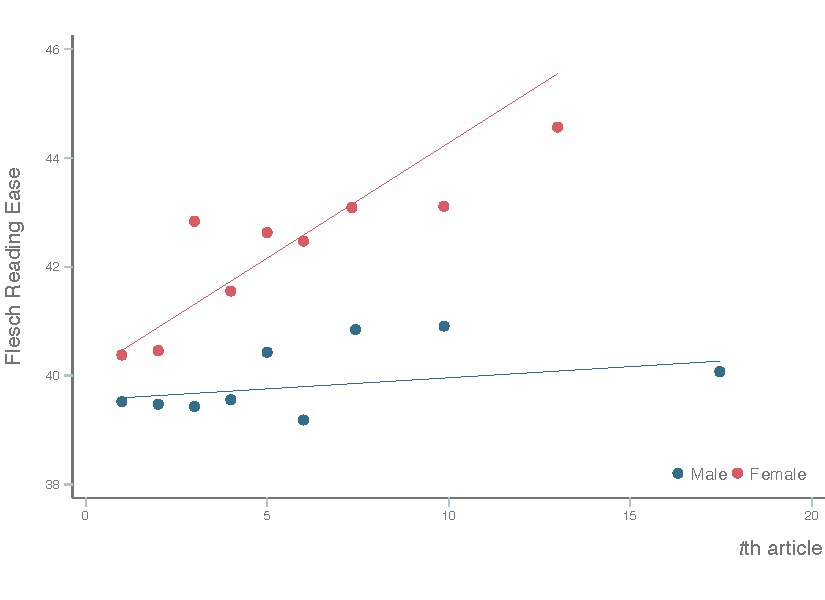
\includegraphics[width=12.3cm,trim=0cm 0.7cm 0cm 0.75cm,clip]{0-images/generated/Figure-4.pdf}
		\floatfoot{\tiny \textit{Notes}. Sample 16,055 observations. Binned scatter plot of abstract readability for authors' first, second, \textit{etc.} top-four paper.}
	}
\end{figure}

I first consider whether female-authored papers are accepted more often than male-authored papers (Condition 3). The articles in my data have already been published, so I cannot analyse gender differences in acceptance rates. Nevertheless, the topic has been extensively studied elsewhere. A recent study of four comparable journals suggests that exclusively male- and female-authored manuscripts receive a revise and resubmit decision 8 and 6 percent of the time, respectively~\citep{Card2020}.  \citet{Blank1991} found that 12.7 and 10.6 percent of male- and female-authored papers were accepted at the \emph{AER}. A study of \emph{JAMA}'s editorial process indicated that 44.8 percent of referees accept male-authored papers as is or if suitably revised; 29.6 percent summarily reject them. Corresponding figures for female-authored papers were 38.3 and 33.3 percent~\citep{Gilbert1994}. Studies from other disciplines find female-authored papers subjected to single-blind peer review are accepted less often than would be expected by chance~\citep{McGillivray2018,Handley2015}. There appear to be no gender differences in acceptance rates to NBER's Summer Institute ~\citep{Chari2017}. See \aref{appendixacceptance} for a table summarising these and other studies.

As for Conditions 1 and 2, women write more clearly than men (Condition 1) and their future papers are more readable than their past papers (Condition 2). As shown in \autoref{underrepresentation}, female-authored abstracts are 1–6 percent more readable than those by men. \autoref{figure7} plots an author's Flesch Reading Ease score against $t$, where $t=1$ for his first top-four publication, $t=2$ for his second, \emph{etc.} As $t$ increases, women's readability improves whereas men's does not.\footnote{As shown in \aref{appendixseuempirical}, women's average readability scores are 1--5 percent higher than the readability of their first papers, their latest papers 1--7 percent higher. For a man, however, his average and last papers are more poorly written than his first.}

\autoref{tableH2_FemRatio} presents the marginal effect on female ratio (papers with fewer than 50 percent female authors are classified as male, see \autoref{gender}) for female authors ($\beta_1$) from estimating \autoref{equationX} on subsamples of authors with $t=1$, $t=2$, \emph{etc.}:\begin{equation}\label{equationX}
	R_{it}=\beta_0+\beta_1\,\text{female ratio}_{it}+\text{female ratio}_{it}\times\text{male}_i+\bm\uptheta\,\vect{X}_{it}+\varepsilon_{it},
\end{equation}where $R_{it}$ is the readability score for author $i$'s $t$th top-four publication, gender enters twice, $\text{male}_i$ and $\text{female ratio}_{it}$, to account for $i$'s sex and the sex of his co-authors, $\vect X_{it}$ is a vector of observable controls and $\varepsilon_{it}$ is the error term.

\begin{table}
    \footnotesize
    \centering
    \begin{threeparttable}
        \caption{Gender gap in readability at increasing \(t\)}
        \label{tableH2_FemRatio}
        \begin{tabular}{p{3cm}S@{}S@{}S@{}S@{}S@{}S@{}S@{}}
            \toprule
            &{\(t=1\)}&{\(t=2\)}&{\(t=3\)}&{\(t=4\text{--}5\)}&{\(t\ge6\)}&{All}\\
            \midrule
            Flesch                        &        0.72   &        1.91*  &        4.64***&        3.24   &        2.69   &        2.24***\\
                                          &      (0.75)   &      (0.99)   &      (1.50)   &      (2.31)   &      (2.01)   &      (0.74)   \\
            Flesch-Kincaid                &        0.07   &        0.23   &        1.04***&        0.72   &        0.46   &        0.29*  \\
                                          &      (0.19)   &      (0.25)   &      (0.25)   &      (0.44)   &      (0.40)   &      (0.16)   \\
            Gunning Fog                   &        0.21   &        0.51*  &        1.29***&        0.99** &        0.62   &        0.53***\\
                                          &      (0.21)   &      (0.28)   &      (0.33)   &      (0.46)   &      (0.41)   &      (0.19)   \\
            SMOG                          &        0.15   &        0.39** &        0.81***&        0.73*  &        0.42   &        0.42***\\
                                          &      (0.14)   &      (0.19)   &      (0.24)   &      (0.38)   &      (0.29)   &      (0.13)   \\
            Dale-Chall                    &        0.04   &        0.05   &        0.23*  &        0.37*  &        0.42*  &        0.15** \\
                                          &      (0.07)   &      (0.10)   &      (0.13)   &      (0.20)   &      (0.23)   &      (0.07)   \\
            \midrule
            No. observations              &       6,874   &       2,827   &       1,675   &       1,906   &       2,773   &      12,008   \\
            \midrule
            Editor effects       &           {\ding{51}}   &           {\ding{51}}   &           {\ding{51}}   &           {\ding{51}}   &           {\ding{51}}   &           {\ding{51}}   \\
            Blind review                  &           {\ding{51}}   &           {\ding{51}}   &           {\ding{51}}   &           {\ding{51}}   &           {\ding{51}}   &               \\
            Journal\(\times\)Year effects          &           {\ding{51}}   &           {\ding{51}}   &           {\ding{51}}   &           {\ding{51}}   &           {\ding{51}}   &           {\ding{51}}   \\
            \(N_j\)                       &           {\ding{51}}   &           {\ding{51}}   &           {\ding{51}}   &           {\ding{51}}   &           {\ding{51}}   &           {\ding{51}}   \\
            Institution effects           &           {\ding{51}}   &           {\ding{51}}   &           {\ding{51}}   &           {\ding{51}}   &           {\ding{51}}   &           {\ding{51}}   \\
            Quality controls              &          {\(\text{\ding{51}}^3\)}   &          {\(\text{\ding{51}}^3\)}   &          {\(\text{\ding{51}}^3\)}   &          {\(\text{\ding{51}}^3\)}   &          {\(\text{\ding{51}}^3\)}   &          {\(\text{\ding{51}}^1\)}   \\
            Native speaker                &           {\ding{51}}   &           {\ding{51}}   &           {\ding{51}}   &           {\ding{51}}   &           {\ding{51}}   &           {\ding{51}}   \\
            \bottomrule
        \end{tabular}
        \begin{tablenotes}
            \tiny
            \item \textit{Notes}. \(\beta_1\) from FGLS estimation of~\autoref{equationX}. First column restricts sample to authors' first top-four publication (\(t=1\)), second column to their second (\(t=2\)), \textit{etc.} Regressions weighted by \(1/N_j\). Standard errors (in parentheses) adjusted for two-way clustering (editor and author) and cross-model correlation. Final column estimates from an unweighted population-averaged regression; error correlations specified by an auto-regressive process of order one and standard errors (in parentheses) adjusted for one-way clustering on author. Quality controls denoted by \(\text{\ding{51}}^1\) include citation count (asinh), \(\text{max. }T\) fixed effects (author prominence) and \(\text{max. }t\) (author seniority); \(\text{\ding{51}}^3\) includes citation count (asinh) and \(\text{max. }t\), only. The variable "female ratio" defines papers with a strict minority of female authors as male-authored; for papers with 50 percent or more female authors, it is the ratio of female authors on a paper (see~\autoref{gender} for more details). ***, ** and * statistically significant at 1\%, 5\% and 10\%, respectively.
        \end{tablenotes}
    \end{threeparttable}
\end{table}

All figures in \autoref{tableH2_FemRatio} agree---women write better---but the magnitude and significance of that difference increases as $t$ increases. Between $t=1$ and $t=2$, the gap marginally widens but is not significant. After that, it triples (at least); the increase is significant ($p<0.05$) for all five scores (\aref{appendixequality}). At higher publication counts, figures are less precisely estimated and smaller than in column 3, but still noticeably larger than estimates in columns 1 and 2.\footnote{Only 40 female authors have 4--5 publications in the data; just 28 have six or more.}

\subsection{Quantifying the counterfactual}
\label{quantification}

Evidence in the previous section suggests women satisfy \autoref{Theorem1}'s three conditions relative to men, on average. However, included controls undoubtedly fail to fully account for differences in the non-readability aspects of men's and women's papers (Assumption 2). Furthermore, concluding that higher standards are present actually requires that all three of \autoref{Theorem1}'s conditions hold for the same author---that is, the same woman must write better than an equivalent man, not be accepted at rates higher than he is \emph{and} raise the quality of her writing over time.

In this section, I attempt to improve my estimates in both respects by restricting the sample to authors with three or more top-four publications. I then match observably similar male and female economists based on characteristics that predict the topic, novelty and quality of their research. Within-person readability comparisons are used to determine if Condition 2 was satisfied for each author in a matched pair. Between-person comparisons after authors gain experience in peer review are used to establish whether Condition 1 was satisfied for the male or female member. I then use these results to construct a counterfactual estimate of the impact higher standards have played in women's readability choices.

\subsubsection{Theoretical strategy}
\label{matchingtheory}

To understand the counterfactual analysis, note that $i$'s optimal choice of readability (defined in \autoref{eq:EU}) can be formulated as a binary decision problem. Specifically, $i$ initially faces the following choice: he can either ignore the impact readability has on his acceptance rate entirely and simply set $R_{it}$ so that marginal cost equals the marginal benefit of the intrinsic satisfaction he derives from writing readable papers (\emph{i.e.}, $R_{it}=R_i^\star$ where $R_i^\star$ solves $c_i'(R)=\phi_i'(R)$); alternatively, he can chase after higher acceptance rates and set $R_{it}>R_i^\star$. If the latter option is chosen, then $i$ optimally minimises $R$ conditional on acceptance rate---\emph{i.e.}, he sets $R_{it}$ just equal to the readability threshold of the last review group he believes will accept his paper. Thus, $R_{it}=\widetilde R_i^{\bar s} + e_{it}$, where $e_{it}$ is the error in $i$'s time $t$ beliefs about $\widetilde R_i^{\bar s}$ and $\bar s$ is the toughest review group to accept $i$'s papers.

Suppose $i$ satisfies the assumptions and conditions of \autoref{Theorem1} relative to $k$ and assume that at time $t'$ $i$ and $k$ are sufficiently experienced in peer review to ensure that $e_{it}$ and $e_{kt}$: (i) are on a path converging to zero (\emph{i.e.}, both getting closer and closer to zero each time $i$ and $k$ go through another round of peer review); and (ii) have already converged to one another (\emph{i.e.}, $e_{it}=e_{kt}$). When these assumptions hold, \autoref{Corollary1} suggests a conservative measure of the impact external factors have on $i$'s time $t'$ readability choice. It is proved in \aref{appendixproofs}.

\begin{corollary}\label{Corollary1}
	Let $i$ satisfy the assumptions and conditions of \autoref{Theorem1} relative to $k$ and assume that for all $t\ge t'$:
	\begin{enumerate}[label=Assumption \arabic*., leftmargin=*, widest*=2, start=4]
		\item $e_{it}=e_{kt}$.
		\item $e_{it}$ and $e_{kt}$ are on a path converging to zero.
	\end{enumerate}
	Then~\autoref{eq:correq1} is a conservative estimate of the impact higher standards play in $i$'s time $t'$ readability choice:
	\begin{equation}
		D_{ik}\equiv R_{it'}-\max\left\{R_{it''},R_{kt'}\right\},
		\label{eq:correq1}
	\end{equation}
	where $R_{it''}$ is the readability of $i$'s time $t''<t'$ paper, as defined in~\autoref{Theorem1}, Condition 2.
\end{corollary}

$D_{ik}$ represents a lower bound on the difference between $i$'s time $t'$ optimal readability score given he's held to higher standards than $k$ (\emph{i.e.}, $R_{it'}$) and the readability score he would have chosen had be been subject to the same standards as $k$ (\emph{i.e.}, $R\le\max\{R_{kt'},R_{it''}\}$). The intuition behind it is simple. First note that it is never optimal for $i$ to choose an $R$ less than $R_i^\star$. Since $i$ already chose $R_{it''}<R_{it'}$ (\autoref{Theorem1}'s Condition 2), that must mean that $R_i^\star\le R_{it''}$. For all $R>R_i^\star$, $i$ prefers to minimise $R$ conditional on acceptance rate, thus, $i$ prefers any $R\in[R_{it''},R_{it'})$ to $R_{it'}$ if it achieves the same acceptance rate as $R_{it'}$. Furthermore, from Condition 3, we know that $i$'s acceptance rate at $R_{it'}$ is identical to $k$'s acceptance rate at $R_{kt'}$. Suppose $R_{kt'}<R_{it''}$. If $i$ and $k$ were subject to identical standards, then $i$'s acceptance rate a $R_{it'}$ would be the same as his acceptance rate at $R_{kt'}$ and therefore also the same as his acceptance rate at $R_{it''}$. Because it may be that $R_{kt'}<R_i^\star\le R_{it''}$, $i$ does not necessarily prefer $R_{kt'}$ to $R_{it''}$, conditional on acceptance rate. We can, however, conclude that $i$ would, at the very least, prefer $R_{it''}$ to $R_{it'}$. Suppose $R_{it''}\le R_{kt'}$. As before, $i$'s acceptance rate at $R_{it'}$ is the same as $k$'s acceptance rate at $R_{kt'}$, but it is no longer necessarily the case that $i$'s acceptance rate at $R_{it''}$ is the same as $k$'s acceptance rate at $R_{kt'}$. Thus, if both were subject to the same standards, then $i$ would, at the very least, prefer $R_{kt'}$ to $R_{it'}$.

\subsubsection{Estimation strategy}
\label{matchingestimation}

Implementing \autoref{Corollary1} first requires that measurement occurs at time $t'$---\emph{i.e.}, a point at which authors are sufficiently experienced for Assumptions 4 and 5 to hold. I assume this point occurs at or before authors' third top-four paper. Authors with one or two top-four publications are probably tenured and well-established in their fields. By publication three, all frequently referee (and some edit) prestigious economics journals. I assume this accumulated experience means: (a) equivalent authors are equally accurate about the standards they are being held to and remaining errors are no longer gender specific; and (b) those errors are getting smaller and smaller each time authors go through another round of peer review.

Additionally, in order to estimate $D_{ik}$, \autoref{Theorem1}'s Assumptions 1--3 must also hold. Most critically, Assumption 2 requires that $i$'s and $k$'s papers are identical with respect to topic, novelty and overall quality. I attempt to satisfy this assumption by matching every female author with three or more top-four publications to her closest male counterpart. Matches were made using a Mahalanobis procedure with the following co-variates: (1) maximum citation count over $t$; (2) institutional rank at $t=1$; (3) fraction of papers published per decade; (4) fraction of papers published by each journal; and (5) number of articles per primary \emph{JEL} category.\footnote{Two notes on co-variate choice. First, I eschew mean, median and minimum citation counts in favour of the maximum on the assumption that an author's ``quality'' is principally a function of his best paper. Second, most people are at top ranked institutions by $t=3$; by matching on institutions at $t=1$, I try to pair authors with similar career paths.} Co-variate balance pre- and post-match are shown in \aref{appendixmatchingbalance}. \aref{appendixmatchingnames} lists each matched pair.

Assume authors are indeed well-matched and also sufficiently experienced at $t=3$. Then under ideal circumstances, comparing $R_{i3}$ to $R_{i1}$ determines the impact information (as proxied for by experience) has on readability, conditional on gender (Condition 2); comparing $R_{i3}$ to $R_{k3}$ determines the impact of gender, conditional on information (Condition 1). Because of co-authoring, however, circumstances are not ideal. In particular, co-authoring means that article gender is neither fixed over $t$ conditional on $i$, nor is $i$'s and $k$'s experience---and hence information---necessarily identical at time $t=3$. I attempt to account for this by predicting $i$'s $t$th paper readability had it only been co-authored with members of $i$'s same sex. To do so, I reconstruct $i$'s time $t$ readability choice at female ratio equal to 1 for women and 0 for men using errors and coefficients from OLS estimation of \autoref{equation14} in the gender and time appropriate subsample of authors:\footnote{More specifically, I separately estimate \autoref{equation14} in the following four subsamples: (i) female authors at $t=1$; (ii) male authors at $t=1$; (iii) female authors at $t=3$; (iv) male authors at $t=3$. I then generate $\widehat R_{it}$ using the appropriate coefficients and errors for each author: (i) $\widehat R_{i1}=\alpha_{1f}+\beta_{1f}+\varepsilon_{i1}$ for a female $i$ at $t=1$; (ii) $\widehat R_{i1}=\alpha_{1m}+\varepsilon_{i1}$ for a male $i$ at $t=1$; \emph{etc.}}\begin{equation}\label{equation14}
	\widehat R_{it} = \alpha_{tg_i} + \beta_{tg_i}\,\text{female ratio}_{it} + \varepsilon_{it},
\end{equation}where $g_i=m,f$ if $i$ is male or female, respectively, ``female ratio'' defines papers with a strict minority of female authors as male-authored; for papers with 50 percent or more female authors, it is the ratio of female authors on a paper (see \autoref{gender} for more details) and $\varepsilon_{it}$ is the estimated error term. As long as $\varepsilon_{it}$ does not partially correlate with a paper's ratio of female authors conditional on $t$ and $g_i$, then $\widehat R_{it}$ provides an unbiased prediction of $R_{it}$. Regression output from \autoref{equation14} is shown in \aref{appendixreconstruction}. To adjust for the degrees of freedom lost when generating $\widehat R_{it}$, standard errors in subsequent calculations are inflated by 1.05. \aref{appendixseur} presents results using the unadjusted, observed $R_{it}$ instead of $\widehat R_{it}$.

\subsubsection{Results}
\label{matchingresults}

\begin{table}
    \footnotesize
    \centering
    \begin{threeparttable}
        \caption{\(D_{ik}\) (\autoref{Corollary1})}
        \label{table8_base}
        \begin{tabular}{p{3cm}S[table-format=3.3]@{}S[table-format=3.3]@{}S[table-format=3.2]@{}S[table-format=4.3]@{}S[table-format=3.3]@{}S[table-format=3.1]@{}S@{}}
            \toprule
            &\multicolumn{3}{c}{{\crcell[b]{Higher standards for\\[-0.1cm]women (\(D_{ik}>0\))}}}&\multicolumn{3}{c}{{\crcell[b]{Higher standards for\\[-0.1cm]men (\(D_{ik}<0\))}}}&{{Mean \(D_{ik}\)}}\\\cmidrule(lr){2-4}\cmidrule(lr){5-7}\cmidrule(lr){8-8}&{{Mean}}&{{S.D.}}&{{\(N\)}}&{{Mean}}&{{S.D.}}&{{\(N\)}}&{{All obs.}}\\
            \midrule
            Flesch                        &        9.39&        7.80&          52&       -4.96&        5.50&          27&        2.92***\\
                                          &            &            &            &            &            &            &      (0.79)   \\
            Flesch Kincaid                &        1.65&        1.40&          63&       -1.30&        1.36&          23&        0.66***\\
                                          &            &            &            &            &            &            &      (0.16)   \\
            Gunning Fog                   &        2.31&        1.85&          55&       -1.55&        1.74&          24&        0.79***\\
                                          &            &            &            &            &            &            &      (0.20)   \\
            SMOG                          &        1.74&        1.42&          51&       -1.00&        1.12&          27&        0.51***\\
                                          &            &            &            &            &            &            &      (0.15)   \\
            Dale-Chall                    &        0.83&        0.67&          61&       -0.67&        0.50&          25&        0.29***\\
                                          &            &            &            &            &            &            &      (0.08)   \\
            \bottomrule
        \end{tabular}
        \begin{tablenotes}
            \tiny
            \item \textit{Notes}. Sample 121 matched pairs. First and second panels display conditional means, standard deviations and observation counts of \(D_{ik}\) (\autoref{Corollary1}) from subpopulations of matched pairs in which the woman or man, respectively, satisfies Conditions 1 and 2. Male scores are subtracted from female scores, meaning \(D_{ik}\) is, by definition, positive in panel one and negative in panel two. Third panel averages \(D_{ik}\) over all matched pairs (\(D_{ik}=0\) whenever neither member simultaneously satisfies Conditions 1 and 2). Estimates are weighted by frequency observations are used in a match; degrees-of-freedom corrected standard errors in parentheses. ***, ** and * statistically significant at 1\%, 5\% and 10\%, respectively.
        \end{tablenotes}
    \end{threeparttable}
\end{table}

\autoref{table8_base}'s first and second panels display means and standard deviations of $D_{ik}$ (\autoref{eq:correq1}) for matched pairs where one member satisfies both Conditions 1 and 2 relative to the other member. In the first panel, the female member does; in the second, it's the male member. Male scores are subtracted from female scores, so $D_{ik}$ is, by definition, positive in panel one and negative in panel two.

Results in \autoref{table8_base} suggest that Conditions 1 and 2 were satisfied for the same author in 65 percent of matched pairs. In two-thirds of those, the member who satisfied them was female. Moreover, $D_{ik}$'s magnitude is (on average) 1.5 times larger in matched pairs where the female member satisfied Conditions 1 and 2 compared to pairs in which the male member did. \autoref{figure8_base} emphasises this point. It displays the distribution of $D_{ik}$: when the evidence suggests a man is subject to higher standards, $D_{ik}$ clusters close to zero; when it suggests the woman is, $D_{ik}$ is far more spread out.

\autoref{table8_base}'s final panel averages $D_{ik}$ over all observations, setting $D_{ik}=0$ in matched pairs where neither member satisfied Conditions 1 and 2. Mean $D_{ik}$ is consistently positive and significant indicating that higher standards are, on average, directed at women: women write about 3 points more readably on the Flesch Reading Ease scale; according to the four grade-level scores, their writing takes around 4--9 fewer months of schooling to understand than it would if they weren't subject to higher standards. Percentage-wise, these results suggest that higher standards mean women write, on average, 5 percent more readably than they otherwise would.

I emphasis, however, that these conclusions are predicated on several strong assumptions; if any are violated, then higher standards against women cannot be inferred from \autoref{table8_base} and \autoref{figure8_base}. First, and most critically, $i$ and $k$ must be identical with respect to topic, novelty and overall quality. Second, at time $t=3$ authors must have learned enough about the process of peer review for Assumptions 4 and 5 in \autoref{Corollary1} to hold. Finally, \autoref{equation14} must accurately predict the readability of $i$'s and $k$'s papers as if they had been co-authored by members of their same sex. Please see \aref{appendixmatchinglimitations} where I discuss the validity and robustness of these assumptions in more detail.

\begin{figure}
	
	\floatbox{figure}[\FBwidth]
	{
		\caption{Distributions of \(D_{ik}\) (\autoref{Corollary1})}\label{figure8_base}
	}
	{
		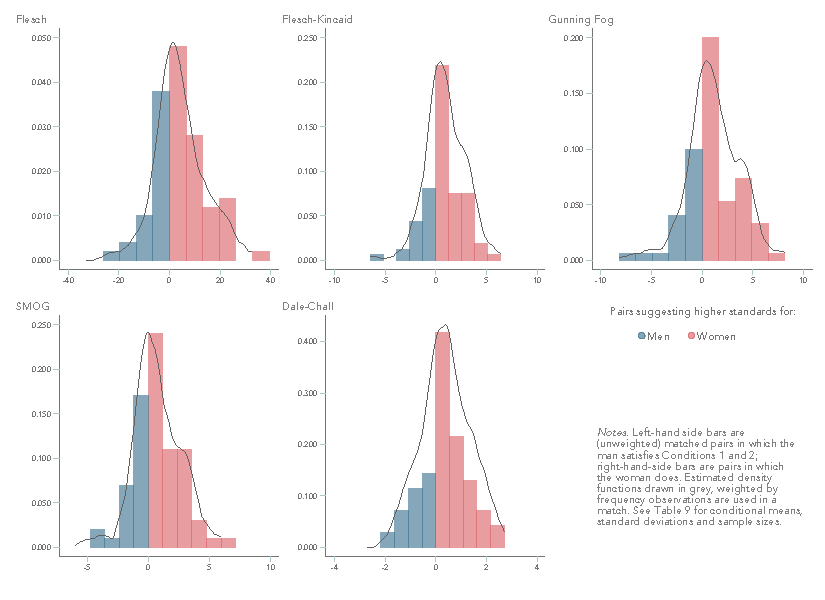
\includegraphics[width=12.3cm]{0-images/generated/Figure-5-base.pdf}
	}
\end{figure}

\subsection{Understanding how women respond to higher standards}
\label{indirecteffect}

Women can respond to higher standards in two different ways: immediately (direct effect) and pre-emptively (feedback effect). As emphasised in \autoref{seumodel}, the weight of each effect likely depends on authors' information about---hence experience with---the peer review process. In this section, I illustrate the evolution of the relative importance of each by comparing papers pre- and post-review as authors' publication counts rise. To do so, I estimate the following equation:\begin{equation}\label{equation15}
	R_{itm} =	\beta_0 + \beta_1\,\text{female ratio}_{it} + \beta_2\,\text{female ratio}_{it}\times t_{it} + \beta_3\,t_{it} + \bm\uptheta\,\vect X_{it} + \varepsilon_{it},
\end{equation}where $m=W,P$ for working papers and published articles, respectively, ``female ratio'' defines papers with a strict minority of female authors as male-authored; for papers with 50 percent or more female authors, it is the ratio of female authors on a paper (see \autoref{gender} for more details), $t_{it}$ is author $i$'s number of top-four papers at time $t$, $\vect X_{it}$ is a vector of observable controls and $\varepsilon_{it}$ is the error term. 

Results from estimating \autoref{equation15} are shown in \autoref{figure9} and \autoref{table9}. In \autoref{figure9}, hollow circles denote draft readability; solid diamonds reflect readability in the final, published versions of those same papers. Dashed lines trace readability as papers undergo peer review (direct effect) and correspond to estimates in the first panel of \autoref{table9}. \autoref{table9}'s second panel shows the marginal effect of female ratio (papers with fewer than 50 percent female authors are classified as male) for each version of a manuscript over increasing $t$. Estimates for published articles correspond to the difference between pink and blue diamonds in \autoref{figure9}; estimates for draft papers represent feedback effects and correspond to differences between hollow circles. Difference-in-differences are shown in the final panel of \autoref{table9}.

\begin{figure}
	
	\floatbox{figure}[\FBwidth]
	{
		\caption{Readability of authors' $t$th paper (draft and final)}\label{figure9}
	}
	{
		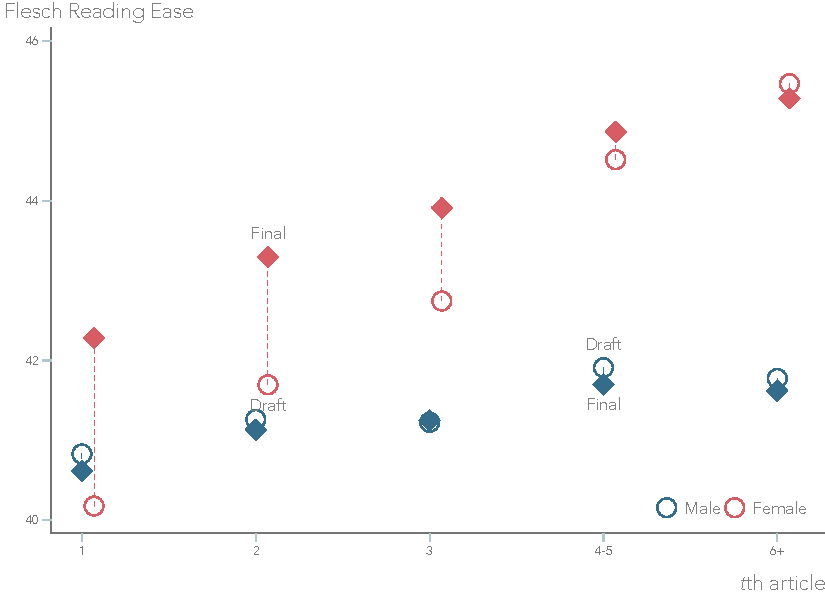
\includegraphics[width=12.3cm]{0-images/generated/Figure-6.pdf}
		\floatfoot{\tiny \textit{Notes}. Flesch Reading Ease marginal mean scores for male (blue) and female (pink) authors' $t=1$, $t=2$, \textit{etc.} top-four publications. Hollow circles denote draft readability; solid diamonds denote readability in published versions of the same papers. See~\autoref{table9} for point estimates, standard errors and further estimation details.}
	}
\end{figure}

\autoref{figure9} and \autoref{table9} suggest that the gender readability gap in published articles is statistically significant and relatively stable at almost every $t$. At $t=1$, it is formed almost entirely during peer review; by $t\ge4$ is is largely formed prior to submission. That is, gender differences in the direct effect of peer review start off large, positive and significant but as $t$ increases, they gradually go away. For the feedback effect, however, the pattern is reversed. Differences in draft readability do not appear to contribute to the gender gap at $t=1$, but this gap rises as $t$ increases.

\begin{table}
    \footnotesize
    \centering
    \begin{threeparttable}
        \caption{Readability of authors' \(t\)th paper (draft and final)}
        \label{table9}
        \begin{tabular}{p{3cm}S@{}S@{}S@{}S@{}S@{}S@{}}
            \toprule
            &{\(t=1\)}&{\(t=2\)}&{\(t=3\)}&{\(t=4\text{--}5\)}&{\(t\ge6\)}\\
            \midrule
            \multicolumn{6}{l}{\textbf{Predicted \(R_{jP}-R_{jW}\)}}\\
            \quad Women                   &        2.09***&        1.59** &        1.16   &        0.35   &       -0.18   \\
                                          &      (0.72)   &      (0.71)   &      (0.86)   &      (1.12)   &      (1.46)   \\
            \quad Men                     &       -0.21   &       -0.13   &        0.02   &       -0.21   &       -0.16   \\
                                          &      (0.17)   &      (0.10)   &      (0.09)   &      (0.14)   &      (0.17)   \\
            \midrule\multicolumn{6}{l}{\textbf{Marginal effect of female ratio}}\\
            \quad Published article       &        1.67   &        2.17** &        2.67***&        3.16***&        3.66** \\
                                          &      (1.11)   &      (0.85)   &      (0.86)   &      (1.14)   &      (1.54)   \\
            \quad Draft paper             &       -0.62   &        0.46   &        1.53** &        2.61***&        3.68***\\
                                          &      (1.31)   &      (0.94)   &      (0.75)   &      (0.88)   &      (1.23)   \\
            \midrule
            \textbf{Diff.-in-diff.}&        2.29***&        1.71** &        1.14   &        0.56   &       -0.02   \\
                                          &      (0.76)   &      (0.76)   &      (0.93)   &      (1.20)   &      (1.52)   \\
            \bottomrule
        \end{tabular}
        \begin{tablenotes}
            \tiny
            \item \textit{Notes}. Sample 4,289 observations. Panel one displays magnitude of predicted \(R_{jP}-R_{jW}\) (the direct effect of peer review) for women and men over increasing \(t\). Panel two estimates the marginal effect of an article's female ratio (\(\beta_1+\beta_2\times t\)), separately for draft papers and published articles. Figures from FGLS estimation of~\autoref{equation15}, weighted by \(N_{it}\) (see~\autoref{data}). Control variables include citation count (asinh), \(\text{max. }T\) (author prominence) and \(\text{max. }t\) (author seniority), native speaker and editor and journal-year fixed effects. defines papers with a strict minority of female authors as male-authored; for papers with 50 percent or more female authors, it is the ratio of female authors on a paper (see~\autoref{gender} for more details). Standard errors clustered by editor and robust to cross-model correlation in parentheses. ***, ** and * statistically significant at 1\%, 5\% and 10\%, respectively.
        \end{tablenotes}
    \end{threeparttable}
\end{table}

\subsubsection{Interpretation}
\label{indirecteffectinterpretation}

A number of \emph{tentative} conclusions about the gender readability gap can be made from \autoref{figure9} and \autoref{table9}. First, inexperienced men and women seem to make similar choices in draft readability. This suggests similar initial preferences for and beliefs about the impact of writing well. In one important sense, however, men are still better informed: the standards they believe apply actually do; junior women appear to mistakenly assume similar standards apply to them, too.

Second, experienced men \emph{and} women seem to sacrifice time upfront in order to improve their odds in peer review. By anticipating referees' demands, authors can partially insure themselves against rejection and\slash or excessively long review. The price is having to spend more time revising a manuscript before submitting it. Assuming choices by senior economists express optimal trade-offs with full information, \autoref{figure9} implies little---if any---gender differences in these preferences for insurance. Again, however, higher standards will mean that the price of that insurance is greater for women than it is for men.

Finally, \autoref{figure9} suggests the direct effect of peer review dominates when women have less experience; the feedback effect dominates when they have more experience. This pattern of behaviour implies that women initially underestimate referees' thresholds but learn about them over time and adapt by writing their future papers more readably prior to submission. This last observation suggests inexperienced female economists go through the toughest review, conditional on acceptance. To investigate further, I test the impact of experience on time spent in review by re-estimating \autoref{equation16} on sub-samples of junior and senior authors. Results are displayed in \aref{appendixtimeexp}. They suggest papers by junior women do indeed take longer in review; the gender gap is significantly smaller---albeit still positive---for senior women.

\section{Conclusion}
\label{conclusion}

Most raw numerical counts suggest women produce less than men: female real estate agents list fewer homes~\citep{Seagraves2013}; female lawyers bill fewer hours~\citep{Azmat2017}; female physicians see fewer patients~\citep{Bloor2008}; female academics write fewer papers~\citep{Ceci2014}. When evaluated by narrowly defined quality measures, however, women often outperform: houses listed by female real estate agents sell for higher prices~\citep{Salter2012,Seagraves2013}; female lawyers make fewer ethical violations~\citep{Hatamyar2004}; patients treated by female physicians are less likely to die or be readmitted to hospital~\citep{Tsugawa2016}.

As I argue in this paper, female economists surpass men on another dimension: writing clarity. Abstracts written by women are 1--6 percent more readable than similar abstracts by men. They also become 2--5 percent more readable while under review when referees aren't blinded to authors' identities. Furthermore, the cost to women of revising their papers appears to be much higher than the cost to men: female-authored papers spend 3--6 months longer under review compared to observably equivalent male-authored papers. Finally, it does not appear that women are rewarded for their better writing: recent evidence from a set of comparable journals suggests female-authored papers are accepted at lower rates, conditional on quality~\citep{Card2020}.

To interpret these stylised facts, I model an author's decision-making process as if it were governed by the rational behaviour of women who update their beliefs about the readability thresholds they are held to as they gain experience in peer review. I then derive three testable conditions which can help establish whether higher standards are at all important to the existence and evolution of the gender readability gap: (1) experienced women write better than equivalent men; (2) women improve their writing over time; and (3) female-authored papers are accepted no more often than equivalent male-authored papers.

On average, I find that all three conditions hold: women's writing gradually gets better but men's does not; between authors' first and third published articles, the readability gap increases by up to 12 percent; as already mentioned, female-authored papers are not accepted at higher rates after conditioning on similar co-variates~\citep{Card2020}. I then conduct a counterfactual analysis that exploits within- and between-individual variation in readability among well-published economists. Its results suggest that higher standards lead women to write, on average, 5 percent more readably than they otherwise would.

I emphasis, however, that these conclusions are predicated on several strong assumptions; if any are violated then other hypotheses are also consistent with the data. For example, if matching does not fully account for differences in the non-readability aspects of men's and women's papers, then gender differences in readability may be influenced by gender differences in specialisation over time. Similarly, no control perfectly captures how empirical vs. theoretical a paper is; as a result, the gender gaps I observe may be biased by differences between fields. Additionally, the validity of the counterfactual analysis and the precision of its estimates rely on strong assumptions about men's and women's beliefs and the impact co-authors have on an article's readability.

Higher standards, wherever present, reduce women's labour market opportunities. Work that is evaluated more critically at any point in the production process will be systematically better (holding prices fixed) or systematically cheaper (holding quality fixed). This will reduce women's wages, distort measurements of their productivity and negatively impact their labour market outcomes. For example, if judges require better writing in female-authored briefs, female attorneys must charge lower fees and\slash or under-report hours to compete with men; billable hours and client revenue will decline, making female lawyers appear less productive than they truly are. In academia, higher standards coupled with longer peer review times likely affect women's probability of obtaining tenure.

Unfortunately, there are no easy solutions for addressing higher standards. But least intrusive---and arguably most effective---is simple awareness and constant supervision. I hope journals are challenged to address the tougher standards they likely impose on women, open to policies that transparently monitor them and supportive of research that helps us better understand them.


% Bibliography.
\ifappendixlast
    \begin{SingleSpace}
        \printbibliography[heading=subbibliography]
    \end{SingleSpace}

\clearpage
\begin{appendices}
\begin{refsection}


\section{Proofs}
\label{appendixproofs}


% Lemma 1.
\begin{lemma}\label{Lemma1}
	$\{(r_{0it}, R_{it})\}$ is bounded.
\end{lemma}
\begin{proof}
Consider the sequence of initial readability choices, $\{r_{0it}\}$. I first show that $R_i^\star\le r_{0it}$ for all $t$. Recall $r_{0it}$ is chosen to maximise the author's subjective expected utility in~\autoref{equation9}. It satisfies the following first order condition
\begin{equation}\label{equationA1}
	\int_\Sigma\!\left(\pi_{0it}^s(r_{0it})v_{1it}^s+\Pi_{0it}^s(r_{0it})\frac{\pd v_{1it}^s}{\pd{r_{0it}}}\right)\dd\mu_i+\phi_i'(r_{0it})-c_i'(r_{0it})=0,
\end{equation}
where $v_{1it}^s$ represents \autoref{equation9} evaluated at the optimal $r_{1it}$. $\phi_{i|r_{0it}}(r_{1it})=\phi_i(R_{it})-\phi_i(r_{1it})$ and $c_{i|r_{0it}}(r_{1it})=c_i(R_{it})-c_i(r_{0it})$. Thus,
\begin{align}\label{equationA2}
	\frac{\pd v_{1it}^s}{\pd r_{0it}}&=\pi_{1it}^s(R_{it})u_i+\phi_i'(R_{it})-c_i'(R_{it})-\phi_i'(r_{0it})+c_i'(r_{0it})\nonumber\\
	&=\frac{\pd v_{1it}^s}{\pd r_{1it}}+c_i'(r_{0it})-\phi_i'(r_{0it}).
\end{align}

Since $\phi_i'(R_i^\star)=c_i'(R_i^\star)$, $\pd v_{1it}^s/\pd r_{0it}=\pd v_{1it}^s/\pd r_{1it}$ when evaluated at $r_{0it}=R_i^\star$. The left hand side of~\autoref{equationA1} evaluated at $r_{0it}=R_i^\star$ is correspondingly equivalent to
\begin{equation}\label{equationA3}
	\int_\Sigma\!\left(\pi_{0it}^s(r_{0it})v_{1it}^s+\Pi_{0it}^s(r_{0it})\frac{\pd v_{1it}^s}{\pd r_{1it}}\right)\dd\mu_i.
\end{equation}
$v_{1it}^s$ is non-negative;\footnote{\autoref{equation8} evaluated at $r_{1it}=0$ is non-negative. Since $r_{1it}$ maximises~\autoref{equation8}, $v_{1it}^s$ is likewise non-negative.} optimising behaviour at stage 1 implies $\pd v_{1it}^s/\pd r_{1it}\ge0$: either an $r_{1it}$ exists that satisfies $\pd v_{1it}^s/\pd r_{1it}=0$, or the author chooses $r_{1it}=0$ and $\pd v_{1it}^s/\pd r_{1it}=\pi_{1it}^s(R_{it})u_i$ is non-negative. Thus,~\autoref{equationA3} is non-negative. Since $c_i'(r)<\phi_i'(r)$ for all $r<R_i^\star$, the left-hand side of~\autoref{equationA1} is strictly positive for all $r<R_i^\star$, so $r_{0it}$ must be at least as large as $R_i^\star$.

I now show that $\{r_{0it}\}$ is bounded from above. As $r_{0}$ tends to infinity, authors choose not to make any changes at stage 1. Thus,
\begin{equation}\label{equationA4}
	\lim_{r_0\rightarrow\infty}\,\Pi_{0it}^s(r_0)v_{1it}^s=\overline\Pi_{0it}^s\overline\Pi_{1it}^s u_i,
\end{equation}
where $\overline\Pi_{0it}^s$ and $\overline\Pi_{1it}^s$ are some upper bounds on the author's subjective probability of receiving an R\&R and then being accepted in state $s$ at time $t$. Since both are no more than 1, $u_i$ is finite and $\phi_i(r)-c_i(r)$ is strictly decreasing for all $r>R_i^\star$,
\begin{equation}\label{equationA5}
	\lim_{r_0\rightarrow\infty}\left\{\int_\Sigma\!\Pi_{0it}^s(r_0)v_{1it}^s\,\dd\mu_i+\phi_i(r_0)-c_i(r_0)\right\}=-\infty.
\end{equation}

Similarly, because $\Pi_{0it}^s(r_{0it})\Pi_{1it}^s(R_{it})\le1$ for all $s$ and $\phi_i(r)$ and $c_i(r)$ are finite at all $r<\infty$,~\autoref{equation9} is likewise finite for all $r<\infty$. Thus,
\begin{equation*}
	\sup\left\{\argmax_{r_{0it}}\,\int_\Sigma\!\Pi_{0it}^s(r_{0it})v_{1it}^s\,\dd\mu_i+\phi_i(r_{0it})-c_i(r_{0it})\right\}<\infty,
\end{equation*}
so $\{r_{0it}\}$ is bounded.

It remains to show that $\{R_{it}\}$ is likewise bounded. Since $r_{1it}\ge0$ and $R_{it}=r_{0it}+r_{1it}$, $R_{it}$ is bounded below by $r_{0it}$, which, as just shown, is itself bounded. Additionally, the author opts for $r_{1it}=0$ if~\autoref{equation8} is less than 0 for all $r_{1it}>0$. Since $R_i^\star\le r_{0it}$ and $\Pi_{1it}^s(R_{it})\le1$
\begin{align}\label{equationA6}
&\Pi_{1it}^s(R_{it})u_i+\phi_i(R_{it})-\phi_i(r_{0it})-c_i(R_{it})+c_i(r_{0it})\nonumber\\
&\quad\le u_i+\phi_i(R_{it})-c_i(R_{it}).
\end{align}
\autoref{equationA6} is strictly decreasing in $R$ for all $R\ge R_i^\star$. The author will not choose any $R$ strictly greater than the one that equates~\autoref{equationA6} to 0. Thus, $\{R_{it}\}$ is bounded from above.

Because $\{r_{0it}\}$ and $\{R_{it}\}$ are bounded, the sequence $\{(r_{0it},R_{it})\}$ in $\RR^2$ is likewise bounded. Thus, all is proved.
\end{proof}

% Lemma 2.
\begin{lemma}\label{Lemma2}
	$r_{0i}\le r_{0it}$ and $R_i^s\le R_{it}^s$ for all $t>t''$.
\end{lemma}
\begin{proof}
Bounded infinite sequences have at least one cluster point and at least one subsequence that converges to each cluster point (Bolzano-Weierstrass). Let $\{(r_{0it},R_{it}^{q^\star})\}$ denote the complete subsequence of $\{(r_{0it},R_{it})\}$ in which state $q$ is reached. Thus,
\begin{equation*}
	\left\{\left(r_{0it},R_{it}^{s^\star}\right)\right\}\bigcap\limits_{s^\star\ne q^\star}\left\{\left(r_{0it},R_{it}^{q^\star}\right)\right\}=\varnothing\quad\text{and}\quad\bigcup\limits_{q^\star\in\Sigma}\left\{\left(r_{0it},R_{it}^{q^\star}\right)\right\}=\left\{\left(r_{0it},R_{it}\right)\right\}.
\end{equation*}

Fix state $s$. Because $\Sigma$ is finite, $\{(r_{0it},R_{it}^{s^\star})\}$ likewise forms a bounded infinite sequence and therefore converges to at least one cluster point. Fix one such cluster point, $(r_{0i}, R_i^s)$, and let $\{(r_{0it},R_{it}^s)\}$ denote the subsequence of $\{(r_{0it},R_{it}^{s^\star})\}$ that converges to it.

Consider first the proposition that $R_i^s\le R_{it}^s$ for all $t>t''$. By way of a contradiction, assume $R_{it}^s<R_i^s$ for all $t>t''$ and some fixed $r_{0it}^s$. Thus, $r_{1it}^s<r_{1it+1}^s$ for all $t>t''$. A positive $r_{1it}^s$ implies that $R_{it}^s$ satisfies
\begin{equation}\label{equationA7}
	\pi_{1it}^s(R_{it}^s)=\frac{1}{u_i}\left(c_i'(R_{it}^s)-\phi_i'(R_{it}^s)\right).
\end{equation}

Let $\pi_{1i}^s$ denote the terminal value of $\pi_{1it}^s$ as $t$ tends to $\infty$. $\pi_{1i}^s$ is finite; thus, $\{\pi_{1it}^s\}$ itself converges: if $\widetilde R_i^s<R_i^s$, then $\pi_{1it}^s(R_{it}^s)=0$ for all $t>t''$, where $t''$ has been redefined to assure $\widetilde R_i^s\le R_{it}^s$; if $R_i^s\le\widetilde R_i^s$ and $\pi_{1i}^s(R_i^s)=\infty$, then $\pi_{1i}^s(R)=0$ for all $R>R_i^s$, a contradiction (see~\autoref{Footnote70}). % You previously wrote "A violation of Assumption X." Erin, what the *fuck* is Assumption X? You need to go back and fix this. I think it has something to do with footnote 70---that's at least what I wrote!

Convergence by $\{\pi_{1it}^s\}$ and $\{R_{it}^s\}$ means
\begin{equation*}
	\lim_{t\rightarrow\infty}\,\Big|\pi_{1it+1}^s(R_{it+1}^s)-\pi_{it}^s(R_{it}^s)\Big|=0.
\end{equation*}
Yet~\autoref{equationA7} implies
\begin{align}\label{equationA8}
	&\lim_{t\rightarrow\infty}\,\Big|\pi_{1it+1}^s(R_{it+1}^s)-\pi_{it}^s(R_{it}^s)\Big|\nonumber\\
	&\quad=\lim_{\varepsilon\rightarrow0}\,\frac{1}{u_i}\Big(\left[c_i'(R_{it}^s+\varepsilon)-c_i'(R_{it}^s)\right]-\left[\phi_i'(R_{it}^s+\varepsilon)-\phi_i'(R_{it}^s)\right]\Big)\nonumber\\
	&\qquad=\frac{1}{u_i}\left(c_i''(R_i^s)-\phi_i''(R_i^s)\right),
\end{align}
where $R_{it}^s\rightarrow R_i^s$ guarantees that for all (sufficiently small) $\varepsilon>0$ there exists $R_{it+1}^s=R_{it}^s+\varepsilon$. $u_i>0$, $c_i''(R)>0$ and $\phi_i''(R)<0$ by assumption; thus,~\autoref{equationA8} is strictly positive. According to~\autoref{equationA8}, $\{\pi_{1it}^s\}$ does not converge, a contradiction.

Consider now the proposition that $r_{0i}\le r_{0it}$ for all $t$ past some $t''$. As before, I proceed with a contradiction. Suppose $r_{0it}<r_{0i}$ for all $t>t'$, where $t'$ is large enough that $\widetilde r_{0i}^q\not\in(r_{0it'},r_{0i})$ for all $q\ne s$ and $r_{1it+1}^s\le r_{1it}^s$ for all $s\in\Sigma$.

At time $t$, the author chooses $r_{0it}$. This choice is governed by the first-order condition in~\autoref{equationA1}:
\begin{equation}\label{equationA9}
	K+\mu_i^s\left(\pi_{0it}^s(r_{0it})v_{1it}^s+\Pi_{0it}^s(r_{0it})\frac{\pd v_{1it}^s}{\pd{r_{0it}}}\right)=c_i'(r_{0it})-\phi_i'(r_{0it})
\end{equation}
where $\mu_i^s$ is the probability of drawing state $s$ and $$K=\int_{\Sigma\setminus s}\!\left(\pi_{0it}^q(r_{0it})v_{1it}^q+\Pi_{0it}^q(r_{0it})\frac{\pd v_{1it}^q}{\pd{r_{0it}}}\right)\dd\mu_i$$ is the marginal change in expected stage 1 subjective utility in all states $q\ne s$.

If $r_{1it+1}^s>0$ then $r_{1it}^s>0$. Thus $\pd v_{1it}^s/\pd r_{1it}=0$; from~\autoref{equationA2},~\autoref{equationA9} is equivalent to
\begin{equation}\label{equationA10}
	K+\mu_i^s\pi_{0it}^s(r_{0it})v_{1it}^s=\Big(1-\mu_i^s\Pi_{0it}^s(r_{0it})\Big)\Big(c_i'(r_{0it})-\phi_i'(r_{0it})\Big).
\end{equation}
If $r_{1it}^s=0$ then $r_{1it+1}^s=0$, and $\pd v_{1it}^s/\pd r_{1it}=\pi_{1it}^s(R_{it}^s)u_i$.\footnote{If $r_{1it}^s>0$ and $r_{1it+1}^s=0$, redefine $t'$ as $t'+1$. $r_{1it+1}^s\le r_{1it+1}^s$ for all $t>t'$ precludes $r_{1it}^s=0$ and $r_{1it+1}^s>0$.} In this case,~\autoref{equationA9} is equivalent to
\begin{equation}\label{equationA11}
	K+\mu_i^s\Big(\pi_{0it}^s(r_{0it})v_{1it}^s+\Pi_{0it}^s(r_{0it})\pi_{1it}^s(R_{it}^s)u_i\Big)=c_i'(r_{0it})-\phi_i'(r_{0it}).
\end{equation}

By the monotone convergence theorem, $\{v_{1it}^s\}$ and $\{\Pi_{0it}^s\}$ converge.\footnote{$\pd v_{1it}^s/\pd r_{0it}\ge0$ and $v_{1it}^s$ is bounded below by zero and above by $u_i+\max\{\phi_i(R_i^\star)-c_i(R_i^\star),0\}$. $\pi_{0it}^s(r_{0it})\ge0$ since $r_{0it}<r_{0it+1}$ (by assumption) and $\Pi_{0it}^s$ is bounded by 0 and 1 (by definition).} If $\widetilde r_{0i}^s<r_{0i}$, then $\pi_{0it}^s(r_{0it})=0$ for all $t>t'$, where $t'$ has been redefined to assure $\widetilde r_{0i}^s\le r_{0it}$; if $r_{0i}\le\widetilde r_{0i}^s$, then
\begin{equation}\label{equationA12}
	\lim_{t\rightarrow\infty}\,\Pi_{0it}^s(r_{0it})=\lim_{t\rightarrow\infty}\,\sum_{r\in\Omega_t}\pi_{0it}^s(r)=\pi_{0i}^s(r_{0i}),
\end{equation}
where $\Omega_t=(r_{0it-1},r_{0it}]$. $\pi_{0i}^s(r_{0i})=\infty$ implies $\lim\Pi_{0it}^s=\infty$, which is impossible given $\Pi_{0it}^s$, by definition, is a bounded function. Hence, $\{\pi_{0it}^s\}$ is likewise convergent, so
\begin{align*}
	&\lim_{t\rightarrow\infty}\,\Big|\mu_i^s\left(\pi_{0it+1}^s(r_{0it+1})v_{1it+1}^s-\pi_{0it}^s(r_{0it})v_{1it}^s\right)\Big|\\
	&\quad=\mu_i^s\left(\lim_{t\rightarrow\infty}\pi_{0it+1}^s(r_{0it+1})\lim_{t\rightarrow\infty}v_{1it+1}^s-\lim_{t\rightarrow\infty}\pi_{0it}^s(r_{0it})\lim_{t\rightarrow\infty}v_{1it}^s\right)\\
	&\qquad=0
\end{align*}
and
\begin{align*}
	&\lim_{t\rightarrow\infty}\,\Big|\mu_i^su_i\left(\Pi_{0it+1}^s(r_{0it+1})\pi_{1it+1}^s(R_{it+1}^s)-\Pi_{0it}^s(r_{0it})\pi_{1it}^s(R_{it}^s)\right)\Big|\\
	&\quad=\mu_i^s\,u_i\left(\lim_{t\rightarrow\infty}\,\Pi_{0it+1}^s(r_{0it+1})\lim_{t\rightarrow\infty}\,\pi_{1it+1}^s(R_{it+1}^s)-\lim_{t\rightarrow\infty}\,\Pi_{0it}^s(r_{0it})\lim_{t\rightarrow\infty}\,\pi_{1it}^s(R_{it}^s)\right)\\
	&\qquad=0.
\end{align*}
% where absolute value signs are omitted in the second line of each equation because the right hand side of~\autoref{equationA11} is larger at $t+1$ so aggregated components of the left-hand side must as well.

For the moment, assume there exists $t''$ such that for all $r\in(r_{0it''},r_{0i})$, $K$ is constant.\footnote{Effectively, this assumes $\pi_{0it}^q(r)=0$ for all $r\in(r_{0it''},r_{0i})$ and $q\ne s$ and (i) $\Pi_{0it}^q(r)=0$ for all $q$ in which $r_{0i}<\widetilde r_{0i}^q$; (ii) $\Pi_{0it}^q(r)=1$ and $\pi_{1it}^q(R_{it}^q)=0$ for all $q$ in which $\widetilde r_{0i}^q<r_{0i}$; and (iii) $\widetilde r_{0i}^q\ne r_{0i}$ for any $q$. Collectively, these assumptions imply convergence of $\{\pi_{0it}^q\}$, $\{R_{it}^q\}$ and $\{\pi_{1it}^q\}$ in every state $q\ne s$ and no change to the author's marginal stage 1 objective function given a small increase in $r$ in any state but $s$. } Thus, changes over time to the left-hand sides of~\autoref{equationA10} and~\autoref{equationA11} converge to 0. Yet the right-hand sides of~\autoref{equationA10} and~\autoref{equationA11} do not, since
\begin{equation*}
	\lim_{t\rightarrow\infty}\,\mu_i^s\Pi_{0it}^s(r_{0it})=\mu_i^s\Pi_{0i}^s(r_{0i})
\end{equation*}
is strictly less than 1, where $\Pi_{0i}^s$ is the finite limit of $\{\Pi_{0it}^s\}$, while
\begin{align*}
	&\lim_{t\rightarrow\infty}\,\Big|\left(c_i'(r_{0it+1})-c_i'(r_{0it})\right)-\left(\phi_i'(r_{0it+1})-\phi_i'(r_{0it})\right)\Big|\\
	&\quad=\lim_{\varepsilon\rightarrow0}\,\left(c_i'(r_{0it}+\varepsilon)-c_i'(r_{0it})\right)-\left(\phi_i'(r_{0it}+\varepsilon)-\phi_i'(r_{0it})\right)\\
	&\qquad=c_i''(r_{0i})-\phi_i''(r_{0i})
\end{align*}
is strictly greater than 0, where convergence of $\{r_{0it}\}$ guarantees that for all (sufficiently small) $\varepsilon>0$ there exists $r_{0it+1}=r_{0it}+\varepsilon$.\footnote{Although the change in $1-\mu_i^s\Pi_{0it}^s(r_{0it})$ between time $t$ and $t+1$ converges to 0, it cannot converge faster than $c_i'(r_{0it})-\phi_i'(r_{0it})$ unless $\pi_{0it}^s(r_{0i})=\infty$, which~\autoref{equationA12} shows is not possible.} Thus, a contradiction.
	
Although the contradiction depends on the existence of $t''$, the finite sum of convergent sequences is also convergent. Thus, for any finite number of states in which $\pi_{0it}^q\ne0$ changes to the left-hand sides of~\autoref{equationA10} and~\autoref{equationA11} converge to 0 while changes to their right-hand sides do not. Because the number of states is finite by assumption, this establishes the general contradiction.
\end{proof}

\begin{lemma}\label{Lemma3}
$\Pi_{0it}^s(r_{0it})\rightarrow\bm 1_{0i}^s(r_{0i})$ and $\Pi_{1it}^s(R_{it}^s)\rightarrow\bm 1_{1i}^s(R_i^s)$.
\end{lemma}
\begin{proof}
As established in~\autoref{Lemma2}, $R_i^s\le R_{it}^s$ for all $t>t''$. If $R_i^s<\widetilde R_i^s$ then $R_{it}^s<\widetilde R_i^s$ for all $t>t''$ where $t''$ has been redefined to satisfy the latter inequality. Thus, the paper is rejected for all $t>t''$ and $\Pi_{1it}^s(R)=0$ for all $R\le R_{it''}^s$ and $t>t''$. If $\widetilde R_i^s\le R_i^s$, then $\widetilde R_i^s\le R_{it}^s$ for all $t>t''$ (again $t''$ redefined to satisfy this inequality). Thus, the paper is accepted for all $t>t''$. $\Pi_{1it+1}^s(R)=1$ for all $R\ge R_{it}^s$ and $t>t''$; $\Pi_{1it}^s(R_{it}^s)$ converges to 1 at the limit.

Also from~\autoref{Lemma2}, $r_{0i}\le r_{0it}$ for all $t>t'$. If $r_{0i}<\widetilde r_{0i}^s$, then the paper is rejected at stage 0 for all $t>t'$, where $t'$ is defined so that $r_{0it}<\widetilde r_{0i}^s$ for all $t>t'$. Define $t''>t'$ such that for all $t>t''$, the probability of having reached state $s$ is 1; thus, $\Pi_{it}^s(r_{0it})=0$ for all $t>t''$. If $\widetilde r_{0i}^s\le r_{0i}$, then redefine $t''$ so that $\widetilde r_{0i}^s\le r_{0it}$ for all $t>t''$. The paper is accepted, $s$ is revealed and $\Pi_{0it+1}^s(r)=1$ for all $r\ge r_{0it}$ and $t>t''$; $\Pi_{0it}^s(r_{0i})$ converges to 1 at the limit. Thus, all is proved.
\end{proof}

\begin{lemma}\label{Lemma4}
There exists a unique cluster point of $\{(r_{0it},R_{it}^{s^\star})\}$ for every $s^\star\in\Sigma$.
\end{lemma}
\begin{proof}
Suppose $\{(r_{0it},R_{it}^{s^\star})\}$ has two cluster points: $(r_{0i}',R_i^{s\prime})$ and $(r_{0i}'',R_i^{s\prime\prime})$. Denote their respective convergent subsequences by $\{(r_{0it}',R_{it}^{s\prime})\}$ and $\{(r_{0it}'',R_{it}^{s\prime\prime})\}$. Given the concavity of $\phi_i$ and convexity of $c_i$, a unique readability at each stage maximises~\autoref{equation8} and~\autoref{equation9} for fixed $\Pi_{0it}^s$ and $\Pi_{1it}^s$. Thus, $r_{0i0}'=r_{0i0}''$ and $R_{i0}^{s\prime}=R_{i0}^{s\prime\prime}$ at time 0.
				
Assume at time $t$ the author has chosen $r_{0il}'=r_{0il}''$ and $R_{il}^{s\prime}=R_{il}^{s\prime\prime}$ for all $l<t$; thus, $\Pi_{0it}^{s\prime}(r)=\Pi_{0it}^{s\prime\prime}(r)$ and $\Pi_{1it}^{s\prime}(R)=\Pi_{1it}^{s\prime\prime}(R)$ for all $r$ and $R$, so the author chooses $r_{0it}'=r_{0it}''$ and $R_{it}^{s\prime}=R_{it}^{s\prime\prime}$ at time $t$ as well. By the axiom of induction, $\{(r_{0it}',R_{it}^{s\prime})\}=\{(r_{0it}'',R_{it}^{s\prime\prime})\}$ for all $t$ so $(r_{0i}, R_i^s)$ is unique.\footnote{Note that $r_{0it}$ is chosen before $s$ is realised, meaning $r_{0i}$ is the unique cluster point of $\{r_{0it}\}$ regardless of $s$.} Since the choice of $s$ was arbitrary exists a unique cluster point of $\{(r_{0it},R_{it}^{s^\star})\}$ for every $s^\star\in\Sigma$.
\end{proof}

\begin{lemma}\label{Lemma5}
	Consider two equivalent authors, $i$ and $k$, such that
	\begin{enumerate}
		\item for at least one $t''<t'$, $(r_{0it''},R_{it''})<(r_{0it'},R_{it'})$ and there exists $K''>0$ such that for no $t>t'$, $||(r_{0it},R_{it})-(r_{0it''},R_{it''})||<K''$; and
		\item $(r_{0kt},R_{kt})\le(r_{0it},R_{it})$ for all $s\in\Sigma_{A_{it}}$ and $t>t'$ and there exists $K'>0$ such that for at least one $s\in\Sigma_{A_{it}}$ and no $t>t'$, $||(r_{0it},R_{it})-(r_{0kt},R_{kt})||<K'$.
	\end{enumerate}
	If $\widetilde r_{0i}^s=\widetilde r_{0k}^s$, $\widetilde R_i^s=\widetilde R_k^s$ and $\mu_i^s=\mu_k^s$ for all $s\in\Sigma$, then
\begin{equation}\label{equationA13}
	\int_\Sigma\!\bm1_{0k}^s(r_{0kt})\bm1_{1k}^s(R_{kt})\,\dd\mu_k<\int_\Sigma\!\bm1_{0i}^s(r_{0it})\bm1_{1it}^s(R_{it})\,\dd\mu_i.
\end{equation}
\end{lemma}
\begin{proof}
	Suppose for the moment that $\Sigma_{A_{it}}$ contains only state $q$ and assume $r_{0kt}=r_{0it}$. Since $q$ is the only state in $\Sigma_{A_{it}}$, $R_{kt}^q<R_{it}^q$. As a result,
\begin{equation*}
	\bm1_{0k}^s(r_{0kt})\bm1_{1k}^s(R_{kt}^s)=\bm1_{0i}^s(r_{0it})\bm1_{1i}^s(R_{it}^s)=0\text{ for all } s\ne q,
\end{equation*}
and
\begin{equation}\label{equationA14}
	\bm1_{0k}^s(r_{0kt})\bm1_{1k}^s(R_{kt}^s)\le\bm1_{0i}^s(r_{0it})\bm1_{1i}^s(R_{it}^s)=1\text{ for }s=q.
\end{equation}
If I show that the inequality in~\autoref{equationA14} is strict, then~\autoref{equationA13} is true. By way of a contradiction, assume it holds as an equality. Thus, $\widetilde R_i^q\le R_k^q<R_i^q$, where $R_{kt}^q\rightarrow R_k^q$ and $R_{it}^q\rightarrow R_i^q$ (\autoref{Lemma4}). Together with $R_i^\star\le r_{0it''}<R_i^q$, this implies
\begin{equation}\label{equationA15}
	\lim_{\varepsilon\rightarrow0-}\Pi_{1i}^q(R_i^q+\varepsilon)<1.\footnote{That is, $\Pi_{0i}^q(R)=1$ for all $R\ge R_i^q$. Because he chose $R_i^\star\le R_{it''}<R_i^q$ at some earlier date, the author's marginal benefit from a higher $R$ is decreasing when the probability of acceptance remains constant. Thus, if he optimally chooses $R_i^q>\max\{R_{it''},R_k^q\}$, it must be because there is no smaller $R$ that satisfies~\autoref{equationA7}. This is only possible if there is a jump discontinuity in $\Pi_{0i}^q$ at $R_i^q$, as illustrated in~\autoref{equationA15}.}
\end{equation}

Meanwhile, author $i$ observes author $k$'s prior readability choices, publication history and paper count. From this, he discovers
\begin{equation}\label{equationA16}
	\lim_{N_k\rightarrow\infty}\frac{N_{A_k}}{N_k}=\mu_i^q,
\end{equation}
where $N_{A_k}$ and $N_k$ are author $k$'s accepted and total paper counts, respectively. Because $i$ updates $\Pi_{1it}^s$ when he observes with probability 1 that in state $s$, $k$ is accepted at some $R\ne R_i^s$ (see~\autoref{Footnote64}),~\autoref{equationA16} necessarily implies
\begin{equation*}
	\lim_{\varepsilon\rightarrow0-}\Pi_{1i}^s(R_i^s+\varepsilon)=1,
\end{equation*}
a contradiction.

Similar proofs by contradiction show that the inequality in~\autoref{equationA14} must also be strict when $R_{kt}^q=R_{it}^q$ and $r_{0kt}<r_{0it}$ in state $q$ and when $\Sigma_{A_{it}}$ contains more than one state.
\end{proof}

\begin{proof}[Proof of Corollary 1]
	I first show that~\autoref{equation11} conservatively estimates $D_{ik}$ when $\Sigma_{A_{it}}\subset\Sigma_{A_{kt}}$. Let $r_{0it}<R_{it}$. From~\autoref{equation10} and the definition of $\delta_{1ik}^s$,
	\begin{align}\label{equationA17}
		R_{it} - R_{kt}	&=		\widetilde R_i^s + e_{1it} - \max\left\{R_k^\star,\widetilde r_{0k}^{\overline s_k} + e_{0kt},\widetilde R_k^s + e_{1kt}\right\}\nonumber\\
						&\le	\widetilde R_i^s - \widetilde R_k^s + e_{1it} - e_{1kt}\nonumber\\
						&=	\delta_{1ik}^s + e_{1it} - e_{1kt}.
	\end{align}
	where $\overline s_k$ is the review group in $\Sigma_{A_{kt}}$ for which $\widetilde r_{0k}^s$ is highest. When $R_{it}=r_{0it}$, however,~\autoref{equation10} and the definition of $\delta_{0ik}^s$ instead imply:
	\begin{align}\label{equationA18}
		R_{it} - R_{kt}	&=		\max\left\{R_i^\star, \widetilde r_{0i}^{\overline s_i} + e_{0it}\right\} - \max\left\{R_k^\star,\widetilde r_{0k}^{\overline s_k} + e_{0kt},\widetilde R_k^s + e_{1kt}\right\}\nonumber\\
						&\le	\max\left\{R_i^\star, \widetilde r_{0i}^{\overline s_i} + e_{0it}\right\} - \widetilde r_{0k}^{\overline s_k} - e_{0kt},
	\end{align}
	where $\overline s_i$ is the review group in $\Sigma_{A_{it}}$ for which $\widetilde r_{0i}^s$ is highest. From~\autoref{Theorem1}'s second condition, $R_{it''}<R_{it}$ for some $t''<t$. Thus, $R_{it''}<r_{0it}$. Because $R_i^\star$ is a lower bound on $r_{0it}$ for all $s$ and $t$ (\autoref{Lemma1}), $R_i^\star<r_{0it}$;~\autoref{equationA18} is equivalent to
	\begin{align}\label{equationA19}
		R_{it} - R_{kt}	&\le	\widetilde r_{0i}^{\overline s_i} - \widetilde r_{0k}^{\overline s_k} + e_{0it} - e_{0kt}\nonumber\\
						&=		\delta_{0ik}^{\overline s_i} + \widetilde r_{0k}^{\overline s_i} - \widetilde r_{0k}^{\overline s_k} + e_{0it} - e_{0kt}.
	\end{align}
	$e_{0it}=e_{0kt}$ and $e_{1it}=e_{1kt}$ (by assumption). Because $\Sigma_{A_{it}}\subset\Sigma_{A_{kt}}$, $\widetilde r_{0k}^{\overline s_i}\le\widetilde r_{0k}^{\overline s_k}$ (by definition);~\autoref{equationA19} implies $R_{it}-R_{kt}\le\delta_{0ik}^{\overline s_i}$ if $R_{it}=r_{0it}$. Meanwhile,~\autoref{equationA17} implies $R_{it}-R_{kt}\le\delta_{1ik}^s$ if $r_{0it}<R_{it}$.
	
	It remains to show that~\autoref{equation12} conservatively estimates $D_{ik}$ under \autoref{Theorem1}'s weaker Condition 3. Let $R_{it''}\le R_{kt}$. Differences in $i$ and $k$'s preferences might influence readability---but only up to $R_{it''}$. $R_{it''}<R_{it}$ is motivated by $i$'s desire to increase his acceptance rate. Since $i$'s unconditional acceptance rate is identical to $k$'s, any $s'$ in $\Sigma_{A_{it}}$ but not in $\Sigma_{A_{kt}}$---\textit{e.g.}, because $i$'s utility of acceptance is higher or cost of writing lower---is perfectly offset by some other $s''$ such that---because $s''$ discriminates against $i$---$s''$ is in $\Sigma_{A_{kt}}$ but not in $\Sigma_{A_{it}}$. Thus, $R_{it}-R_{kt}$ remains a conservative estimate $D_{ik}$.
	
	Now let $R_{kt}<R_{it''}$. Since $i$'s unconditional acceptance rate at $R_{it}$ is identical to $k$'s at $R_{kt}$, $k$'s acceptance rate at $R_{it''}$ must be at least as high as $i$'s at $R_{it}$. Without loss of generality, assume they are identical. Preferences are time independent, so holding acceptance rates constant, $i$ prefers $R_{it''}$ to $R_{it}$. A time $t$ choice of $R_{it}$ over $R_{it''}$ reveals a higher probability of acceptance for the former---and a necessarily lower probability of acceptance for $i$ than $k$ at $R_{it''}$. Given $i$ and $k$ are equivalent, this difference is due to $\delta_{0ik}^{\overline s_i}$ or $\delta_{1ik}^s$. $R_{it}-R_{it''}$ is a conservative estimate of $R_{ik}$. Thus, all is proved.

\end{proof}


\clearpage


\section{Readability data coverage}
\label{appendixarticlecount}

\autoref{table1} displays readability data coverage by journal and decade.


\begin{table}[H]
    \footnotesize
    \centering
    \begin{threeparttable}
        \caption{Article count, by journal and decade}
        \label{table1}
        \sisetup{table-figures-decimal=0}
        \begin{tabular}{p{1.5cm}SSSSS}
            \toprule
            {Decade}&{\textit{AER}}&{\textit{ECA}}&{\textit{JPE}}&{\textit{QJE}}&{Total}\\
            \midrule
            1950--59    &            &         120&            &            &         120\\
            1960--69    &            &         343&         184&            &         527\\
            1970--79    &            &         660&         633&           1&        1294\\
            1980--89    &         180&         648&         562&         401&        1791\\
            1990--99    &         476&         443&         478&         409&        1806\\
            2000--09    &         693&         519&         408&         413&        2033\\
            2010--15    &         732&         382&         181&         251&        1546\\
            \midrule
            Total       &        2081&        3115&        2446&        1475&        9117\\
            \bottomrule
        \end{tabular}
        \begin{tablenotes}
            \tiny
            \item \textit{Notes}. Included is every article published between January 1950 and December 2015 for which an English abstract was found (i) on journal websites or websites of third party digital libraries or (ii) printed in the article itself. Papers published in the May issue of \textit{AER} (\textit{Papers \& Proceedings}) are excluded. Final row and column display total article counts by journal and decade, respectively.
        \end{tablenotes}
    \end{threeparttable}
\end{table}
\clearpage


\section{Description of control variables}
\label{appendixcontrols}

\paragraph{Institutions}
\label{appendixcontrolsinstitutions}

For every article I recorded authors' institutional affiliations. Individual universities in U.S. State University Systems were coded separately (\emph{e.g.}, UCLA and UC Berkeley) but think tanks and research organisations operating under the umbrella of a single university were grouped together with that university (\emph{e.g.}, the Cowles Foundation and Yale University). Institutions linked to multiple universities are coded as separate entities (\emph{e.g.}, École des hautes études en sciences sociales).

In total, 1,039 different institutions were identified. For each institution, I count the number of articles in which it was listed as an affiliation in a given year and smooth the average over a five-year period. Institutions are ranked on an annual basis using this figure and then grouped to create fifteen dynamic dummy variables. Institutions ranked in positions 1--9 are assigned individual dummy variables. Those in positions 10--59 are grouped in bins of 10 to form six dummy variables. Institutions ranked 60 or above were collectively grouped to form a final dummy variable. When multiple institutions are associated with an observation, only the dummy variable with the highest rank is used, \emph{i.e.}, the highest-ranked institution per author when data is analysed at the author-level and the highest-ranked institution for all authors when data is analysed at the article-level.

\paragraph{Citations}
\label{appendixcontrolscitations}

I use article citations from \href{https://login.webofknowledge.com/error/Error?Error=IPError&PathInfo=%2F&RouterURL=https%3A%2F%2Fwww.webofknowledge.com%2F&Domain=.webofknowledge.com&Src=IP&Alias=WOK5}{Web of Science}. Unless otherwise mentioned, citation counts are transformed using the inverse hyperbolic sine function (asinh).

\paragraph{Author prominence}
\label{appendixcontrolsprominence}

I generate 37 dummy variables that group authors by their career-total top-five journal (\emph{AER}, \emph{Econometrica}, \emph{JPE}, \emph{QJE} and \emph{REStud}) publications as of December 2015. For example, Jean Tirole forms one group (59 articles); James Heckman and Gene Grossman form another (34 articles).

\paragraph{Author seniority}
\label{appendixcontrolsseniority}

To account for author seniority, I control for an author's number of top-five (\emph{AER}, \emph{Econometrica}, \emph{JPE}, \emph{QJE} and \emph{REStud}) publications at the time a paper was published. For co-authored articles, only the data corresponding to the most prolific author is used.

\paragraph{English fluency}
\label{appendixcontrolsenglish}

To account for English fluency, most regressions include a dummy variable equal to one if an article is co-authored by at least one native (or almost native) English speaker. I assume an author is ``native'' if he: (i) was raised in an English-speaking country; (ii) obtained all post-secondary eduction from English speaking institutions;\footnote{Non-native speakers who meet this criteria have been continuously exposed to spoken and written English since age 18. This continuous exposure likely means they write as well as native English speakers. To qualify as an English-speaking institution, all courses---not just the course studied by an author---must be primarily taught in English. \emph{E.g.}, McGill University is classified as English-speaking; University of Bonn is not (although most of its graduate economics instruction is in English).} or (iii) spoke with no discernible (to me) non-native accent. This information was almost always found---by me or a research assistant---in authors' CVs, websites, Wikipedia articles, faculty bios or obituaries. In the few instances where the criteria were ambiguously satisfied---or no information was available---I asked friends and colleagues of the author or inferred English fluency from the author's first name, country of residence or surname (in that order).

\paragraph{Field}
\label{appendixcontrolsfield}

I create dummy variables corresponding to the 20 primary and over 700 tertiary \emph{JEL} categories to control for subject matter. The \emph{JEL} system was significantly revised in 1990; because exact mapping from one system to another is not possible, I collected these data only for articles published post-reform---about 60 percent of the dataset. Codes were recorded whenever found in the text of an article or on the websites where bibliographic information was scraped. Remaining articles were classified using codes from the American Economic Association's Econlit database.

I additionally categorised each tertiary \emph{JEL} code as either theory\slash methodology, empirical or other. For example, C02 (mathematical methods) and D85 (network formation and analysis: theory) are classified as theory\slash methodology, whereas D12 (consumer economics: empirical analysis) and F14 (empirical studies of trade) are classified as empirical. Tertiary codes that are not distinctly related to empirical or theory\slash methodology---\emph{e.g.}, L29 (firm objectives, organisation and behaviour: general) or O10 (economic development: general)---are classified as ``other''. (Papers published before 1990 are not classified in any category.) \autoref{jel_list} lists the \emph{JEL} codes assigned to each category.

In total, I classified 99 tertiary \emph{JEL} codes as theory\slash methodology, four as empirical and the remaining 756 as ``other''. (Given the small number of distinctly empirical codes, most ``other'' papers are likely empirical papers.) When combined with my 1990--2015 dataset, there are 1,764 theory\slash methodology articles (34 percent), 412 empirical articles (8 percent) and 4,608 ``other'' articles (88 percent). (Given articles can be both theory and empirical, these percentages do not sum to 100 percent.)

\begin{table}
    \footnotesize
    \centering
    \begin{threeparttable}
        \caption{Tertiary \textit{JEL} code classification}
        \label{jel_list}
        \begin{tabular}{lp{13cm}}
            \toprule
            Category&\textit{JEL} codes\\
            \midrule
            Empirical&D12 D22 F14 O47\\
            Theory&B52 C02 C10 C11 C12 C13 C14 C15 C18 C19 C20 C21 C22 C23 C24 C25 C26 C29 C30 C31 C32 C33 C34 C35 C36 C38 C39 C40 C41 C43 C44 C45 C46 C49 C50 C51 C52 C53 C54 C55 C57 C58 C59 C60 C61 C62 C63 C65 C67 C68 C69 C70 C71 C72 C73 C78 C79 C80 C81 C82 C83 C88 C89 C90 C91 C92 C99 D01 D11 D15 D21 D40 D41 D42 D43 D44 D46 D50 D58 D85 D86 E10 E11 E12 E13 E16 E17 E19 E27 E37 E47 F11 F12 F37 F47 J64 O21 O42 R15\\
            Other&A00 A10 A11 A12 A13 A14 A19 A20 A21 A22 A23 A29 A30 A31 A32 A33 A39 B00 B10 B11 B12 B13 B14 B15 B16 B17 B19 B20 B21 B22 B23 B24 B25 B26 B27 B29 B30 B31 B32 B40 B41 B49 B50 B51 B53 B54 B55 B59 C00 C01 C42 C87 C93 D00 D02 D04 D10 D13 D14 D16 D18 D19 D20 D23 D24 D25 D26 D29 D30 D31 D33 D39 D45 D47 D49 D51 D52 D53 D57 D59 D60 D61 D62 D63 D64 D69 D70 D71 D72 D73 D74 D78 D79 D80 D81 D82 D83 D84 D87 D89 D90 D91 E00 E01 E02 E14 E20 E21 E22 E23 E24 E25 E26 E29 E30 E31 E32 E39 E40 E41 E42 E43 E44 E49 E50 E51 E52 E58 E59 E60 E61 E62 E63 E64 E65 E66 E69 E70 E71 F00 F01 F02 F10 F13 F15 F16 F17 F18 F19 F20 F21 F22 F23 F24 F29 F30 F31 F32 F33 F34 F35 F36 F38 F39 F40 F41 F42 F43 F44 F45 F49 F50 F51 F52 F53 F54 F55 F59 F60 F61 F62 F63 F64 F65 F66 F68 F69 G00 G01 G10 G11 G12 G13 G14 G15 G17 G18 G19 G20 G21 G22 G23 G24 G28 G29 G30 G31 G32 G33 G34 G35 G38 G39 G40 G41 G50 G51 G52 G53 G59 H00 H10 H11 H12 H13 H19 H20 H21 H22 H23 H24 H25 H26 H27 H29 H30 H31 H32 H39 H40 H41 H42 H43 H44 H49 H50 H51 H52 H53 H54 H55 H56 H57 H59 H60 H61 H62 H63 H68 H69 H70 H71 H72 H73 H74 H75 H76 H77 H79 H80 H81 H82 H83 H84 H87 H89 I00 I10 I11 I12 I13 I14 I15 I18 I19 I20 I21 I22 I23 I24 I25 I26 I28 I29 I30 I31 I32 I38 I39 J00 J01 J08 J10 J11 J12 J13 J14 J15 J16 J17 J18 J19 J20 J21 J22 J23 J24 J26 J28 J29 J30 J31 J32 J33 J38 J39 J40 J41 J42 J43 J44 J45 J46 J47 J48 J49 J50 J51 J52 J53 J54 J58 J59 J60 J61 J62 J63 J65 J68 J69 J70 J71 J78 J79 J80 J81 J82 J83 J88 J89 K00 K10 K11 K12 K13 K14 K15 K16 K19 K20 K21 K22 K23 K24 K25 K29 K30 K31 K32 K33 K34 K35 K36 K37 K38 K39 K40 K41 K42 K49 L00 L10 L11 L12 L13 L14 L15 L16 L17 L19 L20 L21 L22 L23 L24 L25 L26 L29 L30 L31 L32 L33 L38 L39 L40 L41 L42 L43 L44 L49 L50 L51 L52 L53 L59 L60 L61 L62 L63 L64 L65 L66 L67 L68 L69 L70 L71 L72 L73 L74 L78 L79 L80 L81 L82 L83 L84 L85 L86 L87 L88 L89 L90 L91 L92 L93 L94 L95 L96 L97 L98 L99 M00 M10 M11 M12 M13 M14 M15 M16 M19 M20 M21 M29 M30 M31 M37 M38 M39 M40 M41 M42 M48 M49 M50 M51 M52 M53 M54 M55 M59 N00 N01 N10 N11 N12 N13 N14 N15 N16 N17 N20 N21 N22 N23 N24 N25 N26 N27 N30 N31 N32 N33 N34 N35 N36 N37 N40 N41 N42 N43 N44 N45 N46 N47 N50 N51 N52 N53 N54 N55 N56 N57 N60 N61 N62 N63 N64 N65 N66 N67 N70 N71 N72 N73 N74 N75 N76 N77 N80 N81 N82 N83 N84 N85 N86 N87 N90 N91 N92 N93 N94 N95 N96 N97 O00 O10 O11 O12 O13 O14 O15 O16 O17 O18 O19 O20 O22 O23 O24 O25 O29 O30 O31 O32 O33 O34 O35 O36 O38 O39 O40 O41 O43 O44 O49 O50 O51 O52 O53 O54 O55 O56 O57 P00 P10 P11 P12 P13 P14 P16 P17 P18 P19 P20 P21 P22 P23 P24 P25 P26 P27 P28 P29 P30 P31 P32 P33 P34 P35 P36 P37 P39 P40 P41 P42 P43 P44 P45 P46 P47 P48 P49 P50 P51 P52 P59 Q00 Q01 Q02 Q10 Q11 Q12 Q13 Q14 Q15 Q16 Q17 Q18 Q19 Q20 Q21 Q22 Q23 Q24 Q25 Q26 Q27 Q28 Q29 Q30 Q31 Q32 Q33 Q34 Q35 Q37 Q38 Q39 Q40 Q41 Q42 Q43 Q47 Q48 Q49 Q50 Q51 Q52 Q53 Q54 Q55 Q56 Q57 Q58 Q59 R00 R10 R11 R12 R13 R14 R19 R20 R21 R22 R23 R28 R29 R30 R31 R32 R33 R38 R39 R40 R41 R42 R48 R49 R50 R51 R52 R53 R58 R59 Y10 Y20 Y30 Y40 Y50 Y60 Y70 Y80 Y90 Y91 Y92 Z00 Z10 Z11 Z12 Z13 Z18 Z19 Z20 Z21 Z22 Z23 Z28 Z29 Z30 Z31 Z32 Z33 Z38 Z39\\
            \bottomrule
        \end{tabular}
        \begin{tablenotes}
            \tiny
            \item \textit{Notes}. Table lists of each tertiary \textit{JEL} code assigned to the empirical, theory/methodology and other categories.
        \end{tablenotes}
    \end{threeparttable}
\end{table}

\paragraph{Editorial policy}
\label{appendixcontrolseditorial}

To control for editorial policy, I recorded editor\slash editorial board member names from issue mastheads. \emph{AER} and \emph{Econometrica} employ an individual to oversee policy. \emph{JPE} and \emph{QJE} do not generally name one lead editor and instead rely on boards composed of four to five faculty members at the University of Chicago and Harvard, respectively. \emph{REStud} is also headed by an editorial board, the size of which has been gradually increasing---from two members in the 1970s to 7--8 members today. Members are also located all over the world.

Editor controls are based on distinct lead editor\slash editorial boards---\emph{i.e.}, they differ by at least one member. Among top four journals, 74 groups are formed in this manner. \emph{REStud} adds another 34. Given the size of \emph{Restud}'s editorial board and the fact that members serve fixed 3--4 full-year terms, editorial controls are highly correlated with year fixed effects. Moreover, unlike at \emph{JPE} and \emph{QJE}, editors are not located at the same institution. Thus, editor fixed effects may be less informative about editorial policy at \emph{REStud} than they are for the other four journals.

\paragraph{Family commitments}
\label{appendixcontrolsfamily}

To control for motherhood's impact on revision times, I recorded children's birth years for women with at least one entirely female-authored paper in \emph{Econometrica}. I personally (and, I apologise, rather unsettlingly) gleaned this information from published profiles, CVs, acknowledgements, Wikipedia, personal websites, Facebook pages, background checks and local school district\slash popular extra-curricular activity websites. Exact years were recorded whenever found; otherwise, they were approximated by subtracting a child's actual or estimated age from the date the source material was posted online. In several instances, I obtained this information from acquaintances, friends and colleagues or by asking the woman directly. If an exhaustive search turned up no reference to children, I assumed the woman in question did not have any.

\clearpage

\section{Readability scores}
\label{appendixreadability}

\subsection{Validity}
\label{appendixvalidity}

Advanced vocabulary and complicated sentences are the two strongest predictors of text difficulty~\citep{Chall1995}. Hundreds of readability formulas exploit this relationship. The five most widely used, tested and reliable formulas for adult reading material are the Flesch Reading Ease, Flesch-Kincaid, Gunning Fog, SMOG (Simple Measure of Gobbledegook) and Dale-Chall~\citep{DuBay2004}. Each are listed in \autoref{tab:formulas}.

These five readability scores generally produce similar rankings: the yellow box plot in \autoref{figure2} summarises 169 inter-score correlations found in 26 studies; the median is 0.87. Moreover, they tend to correlate with (i) oral reading fluency, (ii) human judgement, (iii) reading comprehension tests and (iv) the cloze procedure.\footnote{Oral reading fluency is generally measured as the number of words read aloud correctly per minute. The cloze procedure ranks passages of text according to average readers' ability to correctly guess randomly deleted words.} The dark blue box plots in \autoref{figure2} summarise 167 correlations in 38 published cross-validation studies. (See \aref{appendixmetaanalysis} for a list of studies included in the analysis.)

Furthermore, numerous studies have validated readability scores against surrogate measures of reading comprehension. More readable high school and college-level correspondence courses have higher completion rates~\citep{Klare1973}. More readable academic journals enjoy larger readerships~\citep{Richardson1977,Swanson1948}; their most readable articles win more awards~\citep{Sawyer2008} and are downloaded more often~\citep{Guerini2012}. More readable abstracts are also (generally) cited more frequently (see  \citet{Dowling2018,McCannon2019} and \autoref{figure2}). They are also more likely to be published in top-five and other higher ranking journals~\citep{MarinoFages2020}. In a \href{http://lukaspuettmann.com/2017/12/09/voxeu-gobbledygook/}{blog post}, Lukas Püttmann compares abstract readability to page views of \href{http://www.voxeu.org}{VoxEU.org} columns: more readable columns are viewed three percent more often~\citep{Puttmann2017}. Evidence from other studies linking readability and citations is, however, weaker~\citep{Lei2016, Berninger2017,Laband1992}. My own data suggest a positive relationship in papers published after 1990---and particularly those published post--2000---but no relationship before that (\autoref{figure2}).

Thanks to high predictive power and ease of use, readability formulas are widely employed in education, business and government. The U.S. Securities and Exchange Commission encourages clearer financial disclosure forms benchmarked against the Gunning Fog, Flesch-Kincaid and Flesch Reading Ease scores~\citep{Cox2007}. The formulas have also guided readability assessments of, \emph{inter alia}, standardised test questions~\citep{Chall1977,Chall1983}, medical inserts~\citep[\emph{e.g.},][]{Wallace2008}, technical manuals~\citep[\emph{e.g.},][]{Hussin2012,Klare1973}, health pamphlets~\citep[\emph{e.g.},][]{Foster2002,Meade1989} and data security policies~\citep{Alkhurayyif2017}.

In research, readability scores are often used to proxy for ``complexity''.  \citet{Enke2018} controls for language sophistication using the Flesch Reading Ease formula in a study of moral values in U.S. presidential elections.  \citet{Spirling2016} employs the same score to show that British parliamentarians simplified speeches to appeal to less educated voters in the wake of the Great Reform Act. Legal research has found that judges are more reliant on legislative history when interpreting complex legal statutes, as measured by the Flesch-Kincaid formula~\citep{Law2010}. In finance, the scores have linked clarity of financial communication to better firm and market financial health~\citep{Li2008,Biddle2009,Jansen2011}, larger investment and trading volume ~\citep{Miller2010,Thörnqvist2015,DeFranco2015,Lawrence2013} and lower demand for---albeit higher reliability of---outside research by sell-side analysts~\citep{Lehavy2011}. See also  \citet{Loughran2016} for a review of the use of readability scores in finance and accounting research.

\begin{figure}

	\floatbox{figure}[\FBwidth]
	{
		\caption{Readability score validity}\label{figure2}
	}
	{
	\begin{minipage}{0.95\linewidth}
	\begin{tabular}{cc}
		\multicolumn{2}{c}{\includegraphics[trim=0cm 2cm 0cm 1.9cm, clip,width=0.95\linewidth]{0-images/generated/{Figure-D.1-meta}.pdf}}\\
		\includegraphics[width=0.45\linewidth]{0-images/generated/{Figure-D.1-early}.pdf}&\includegraphics[width=0.45\linewidth]{0-images/generated/{Figure-D.1-late}.pdf}\\
	\end{tabular}
	\end{minipage}
		\floatfoot{\tiny\textit{Notes}. Top figure displays box plots of correlations between alternative measures of text difficulty and the Flesch Reading Ease, Flesch-Kincaid, Gunning Fog, SMOG and Dale-Chall readability scores. It includes 336 correlations found in 55 mostly peer reviewed papers. (See~\aref{appendixmetaanalysis} for the list of included studies and information on how they were selected.) Bottom figures plot abstracts' Flesch Reading Ease scores against their articles' citation counts (inverse hyperbolic sine (asinh) transformation) for the samples of top-four (excluding \textit{AER Papers \& Proceedings}) articles published before 1990 (left) and post-2000 (right). Each point represents the mean (in both dimensions) of roughly 170--180 observations. \(^\dagger\)Includes two studies which assessed readability using the Readability Assessment INstrument (RAIN), a comprehensive framework based on 14 variables, \textit{e.g.}, coeherence, writing style, illustrations and typography.}
	}
\end{figure}

\subsection{Measurement error}
\label{appendixmeasurementerror}

Readability scores fail to capture many elements relevant to reading comprehension, including gram\-mar---\emph{e.g.}, active vs. passive tense~\citep{Coleman1964,Coleman1965}---legibility---\emph{e.g.}, typeface or layout---and content---\emph{e.g.}, coherence, organisation and general appeal~\citep{Kintsch1984,Kemper1983,Meyer1982,Armbruster1984}. Nevertheless, ``long sentences generally correspond to complex syntactic structures, infrequent words generally refer to complex concepts, and hard texts will generally lead to harder questions about their content''~\citep[][p. 222]{Kintsch1984}.

Still, readability scores' low causal power raises legitimate concerns about measurement error. As long as this error does not partially correlate with the variable of interest (gender), the analytical results I present in this paper attenuate toward zero (classical measurement error). Unfortunately, they are systematically biased in an unknown direction if it does (non-classical measurement error).

Sources of non-classical measurement error are threefold: (a) grammatical, spelling and transcription errors in the textual input; (b) errors in the estimates of vocabulary complexity and sentence length introduced by automating their calculation; or (c) embodied in the jump from using these two variables to infer readability.

Conditional on accurate calculation, readability scores combine very precise estimates of vocabulary complexity with almost perfect measures of sentence length~\citep[for a discussion, see][]{Chall1995}. The weighted average of these two variables is informative in much the same way that inferences about readability are. Thus, measurement error related to (c) should only shift superficial interpretation of observed gender differences---from ``women are better writers'' to ``women use simpler words and write shorter sentences''---but leave conclusions deduced from them intact.

Nevertheless, I try to minimise measurement error from (c) by using abstracts as textual input. Abstracts are self-contained, universally summarise the research and are the first and most frequently read part of an article~\citep{King2006}. Additionally, they follow a more standardised layout compared to other parts of a manuscript: they are generally surrounded by ample whitespace and most editorial management systems anyway reproduce them in pre-formatted cover pages. These factors suggest a relatively homogenous degree of review across journals and subject matter and limit the impact that physical layout, figures and surrounding text have on readability.

Moreover, prior research suggests authors write in a stylistically consistent manner across the abstract, introduction and discussion sections of a paper. According to an analysis of published education and psychology articles, within-manuscript correlations of Flesch Reading Ease scores range from 0.64 (abstracts vs. introductions) to 0.74 (abstracts vs. discussions)~\citep{Hartley2003b}.  \citet{Plaven-Sigray2017} also found a strong positive correlation using full text articles from several scientific journals. \autoref{figure3} plots abstract readability against the readability of a passage from the introduction for 339 NBER Working Papers eventually published in a top-four journal. It suggests a similarly positive relationship holds in economics, as well.\footnote{For comparison, I randomly assigned abstracts to introductions in 1,000 simulated samples. The average coefficient of correlation between abstract text readability and the readability of a passage of text from a randomly selected introduction was --0.0006 for the Gunning Fog score and 0.0007 for the Flesch-Kincaid score.}

\begin{figure}

	\floatbox{figure}[\FBwidth]
	{
		\caption{Abstract vs. article readability}\label{figure3}
	}
	{
	\begin{minipage}{0.95\linewidth}
	\begin{tabular}{cc}
		\includegraphics[width=0.45\linewidth]{0-images/generated/{Figure-D.2-fleschkincaid}.pdf}&\includegraphics[width=0.45\linewidth]{0-images/generated/{Figure-D.2-gunningfog}.pdf}\\
	\end{tabular}
	\end{minipage}
		\floatfoot{\tiny\textit{Notes}. Figures plot abstract readability against the readability of a 150--200 word passage of text from the introduction of the same paper. $\beta$ is the slope of the regression line (robust standard errors in parentheses). Sample only includes NBER Working Papers eventually published in a top-four economics journal with a heading explicitly titled ``Introduction'' (339 abstract-article pairs). Data are grouped into roughly 20 equal-sized bins; each point represents the mean (in both dimensions) of about 16--17 observations. Non-abstract text kindly provided by Henrik Kleven and Dana Scott~\citep{Kleven2018}. Readability scores calculated using the \texttt{R} \texttt{readability} package.}
	}
\end{figure}

In my opinion, non-classical measurement error from (a) and (b) poses a bigger concern to the identification mapped out in this paper. I have taken several steps to reduce it. First, abstract text is also ideal for calculating readability: 100--200 words containing few score-distorting features of academic writing---\emph{e.g.}, citations, abbreviations and equations~\citep{Dale1948}. Additionally, most abstracts have been previously converted to accurate machine-readable text by digital libraries and bibliographic databases, curbing errors in transcription.

Second, I carefully proofread the text in order to identify (and fix) remaining transcription errors,\footnote{\emph{E.g.}, words in transcribed text are often inappropriately hyphenated---typically because the word was divided at the end of the line in the original text.} eliminate non-sentence-ending full stops, and replace typesetting code---typically used to render equations---with equivalent unicode characters.\footnote{When no exact replacement existed, characters were chosen that mimicked as much as possible the equation's original intent while maintaining the same character and word counts. (Equations in abstracts generally only occur in \emph{Econometrica} articles published before 1980.)} Readability scores were determined using the modified text.

Finally, some programs that calculate scores rely on unclear, inconsistent and possibly inaccurate algorithms to count words and syllables, identify sentence terminations and check whether a word is on Dale-Chall's easy word list~\citep[for a discussion, see][]{Sirico2007}. To transparently handle these issues and eliminate ambiguity in how the scores were calculated, I wrote the Python module \texttt{Textatistic}. Its code and documentation are available on \href{https://github.com/erinhengel/Textatistic}{GitHub}; a brief description is provided in \aref{appendixtextatistic}.

For added robustness, I also re-calculate scores and replicate most results using the \href{https://github.com/trinker/readability}{\texttt{R} \texttt{readability} package} (\aref{appendixalternativereadability}). Coefficients are very similar to---and (to my chagrin) standard errors universally smaller than---those presented in the body of the paper.

\subsection{\texttt{Textatistic}}
\label{appendixtextatistic}

I wrote the Python module \texttt{Textatistic} to transparently calculate the readability scores in this study. The code and documentation are available on \href{https://github.com/erinhengel/Textatistic}{GitHub}; I provide a brief description here.

To determine sentence count, the program replaces common abbreviations with their full text,\footnote{Abbreviations which do not include full-stops are not altered. I manually replaced common abbreviations, such as ``\emph{i.e.}'' and ``U.S.'' with their abbreviated versions, sans full stops.} decimals with a zero and deletes question and exclamation marks used in an obvious, mid-sentence rhetorical manner.\footnote{For example, ``?).'' is replaced with ``).''.} The remaining full stops, exclamation and question marks are assumed to end a sentence and counted.

Next, hyphens are deleted from commonly hyphenated single words such as ``co-author'' and the rest are replaced with spaces, remaining punctuation is removed and words are split into an array based on whitespace. Word count is the length of that array.\footnote{Per \citet{Chall1995}, hyphenated words count as two (or more) words.}

An attempt is made to match each word to one on an expanded Dale-Chall list. The count of difficult words is the number that are not found. This expanded list, available on \href{https://github.com/erinhengel/Textatistic}{GitHub}, consists of 8,490 words. It is based on the original 3,000 words, but also includes verb tenses, comparative and superlative adjective forms, plural nouns, \emph{etc.} It was created by first adding to the Dale-Chall list every conceivable alternate form of each word using Python's Pattern library. To eliminate nonsense words, the text of 94 English novels published online with Project Gutenberg were matched with words on the expanded list. Words not found in any of the novels were deleted.

Syllable counts are based on the C library \texttt{libhyphen}, an implementation of the hyphenation algorithm from \citet{Liang1983}.  \citet{Liang1983}'s algorithm is used by \TeX's typesetting system. \texttt{libhyphen} is employed by most open source text processing software, including OpenOffice.

\subsection{Studies included in meta analysis}
\label{appendixmetaanalysis}

Below are the studies included in the analysis from \autoref{figure2}, which summarises correlations between readability scores and alternative measures of reading comprehension found in other research. A few notes on the criteria for inclusion and how some correlations were determined:

\begin{itemize}
\item I include only documents produced for the U.S. government or published peer reviewed studies---with the exception of the present paper,  \citet{Benoit2017} and results from dissertations that were presented and discussed in a peer reviewed manuscript.

\item I include a small number of studies with correlations between alternative readability measures and the number of words not listed on the Dale-Chall word list. In all other cases, however, correlations with only parts of a score (\emph{e.g.}, syllables per words) are omitted.

\item A few earlier studies calculated and listed various readability measures for many passages of text, but did not report coefficients of correlation between them. I manually calculated these correlations myself.

\end{itemize}


\begin{refsegment}
\nocite{Flesch1948}
\nocite{Powers1958}
\nocite{Klare1952}
\nocite{Benoit2017}
\nocite{Meade1991}
\nocite{Caylor1973}
\nocite{Entin1978}
\nocite{Woods1998}
\nocite{Jongsma1972}
\nocite{Fulcher1997}
\nocite{Lenzner2014}
\nocite{Hengel2017}
\nocite{Harwell1996}
\nocite{Russell1951}
\nocite{Greenfield1999}
\nocite{Crossley2008}
\nocite{Brown1998}
\nocite{Greenfield2004}
\nocite{Crossley2017}
\nocite{Stajner2012}
\nocite{vanOosten2010}
\nocite{Carver1974}
\nocite{Hayes1996}
\nocite{Hull1979}
\nocite{Ley1996}
\nocite{Kincaid1975}
\nocite{Compton2004}
\nocite{Ardoin2005}
\nocite{Janan2014}
\nocite{Cunningham2018}
\nocite{Zheng2017}
\nocite{Clauson2010}
\nocite{Klingbeil1995}
\nocite{McLaughlin1969}
\nocite{King2003}
\nocite{Singh2003}
\nocite{Wells1994}
\nocite{Dale1948}
\nocite{Powell-Smith2001}
\nocite{Chall1995}
\nocite{Dale1934}
\nocite{Gray1935}
\nocite{Lorge1948}
\nocite{Bormuth1966}
\nocite{Harris1976}
\nocite{Miller1974}
\nocite{Froese1971}
\nocite{Lee1966}
\nocite{Guthrie1972}
\nocite{Sullivan1976}
\nocite{Singer1975}
\nocite{Kemper1983}
\nocite{Morris1980}
\nocite{Meade1989}
\nocite{Kanouse1981}

\end{refsegment}
\printbibliography[segment=1,heading=none]
\clearpage


\section{Discussion of potential alternative mechanisms}
\label{appendixalternatives}

A gender readability gap exists. It's still there after including editor, journal and year effects---meaning it's probably not caused by antiquated policies and attitudes, long since overcome. The gap is unaffected by field controls, so it doesn't seem to be related to women researching topics that are easier to explain. Nor does it appear to be caused by factors correlated with gender but actually linked to authors' (or co-authors') competence as economists and fluency in English---if so, institution, native speaker and citation controls would reduce it. They do not.\footnote{I also conducted a primitive surname analysis ~\citep[see][pp. 35--36]{Hengel2016}. It suggests that the female authors in my data are no more or less likely to be native English speakers.}

The gap grows between first draft and final publication and over the course of women's careers, likely precluding inborn advantage and one-off improvements in response to external circumstances unrelated to peer review. This probably also rules out gender differences in (i) biology\slash behaviour---\emph{e.g.}, sensitivity to referee criticism\footnote{While women do appear more \emph{internally} responsive to feedback---criticism has a bigger impact on their self-esteem---available evidence suggests they aren't any more \emph{externally} responsive to it, \emph{i.e.}, women and men are equally likely to change behaviour and alter performance after receiving feedback~\citep{Johnson2002,Roberts1989}.}---or (ii) knowledge about referee expectations. If diligently addressing every referee concern has no apparent upside---acceptance rates are unaffected---and a very clear downside---constant redrafting takes time---even the most oversensitive, ill-informed woman would \emph{eventually} re-examine initial beliefs and start acting like a man, no?\footnote{This statement is especially relevant if the opportunity cost to women for ``wasting'' time on needless tasks is higher---\emph{e.g.}, because of family responsibilities.} Yet this is not what we observe. The largest investments in writing well are made by female economists with greatest exposure to peer review---\emph{i.e.}, those with the best opportunity to update their priors.

Women's papers are more likely assigned female referees~\citep{Abrevaya2012,Gilbert1994}.\footnote{Note that women are only a fraction of all referees---8 percent in 1986~\citep{Blank1991}, 10 percent in 1994~\citep{Hamermesh1994} and 14 percent in 2013~\citep{Torgler2013}.  \citet{Abrevaya2012} report female-authored papers were only slightly more likely to be assigned a female referee between 1986--1994; matching increases between 2000--2008.} If women are more demanding critics, clearer writing could reflect their tougher reviews.\footnote{It's not clear whether women's reports are more critical. A study specific to post-graduate biologists suggests yes~\citep{Borsuk2009}; other studies specific to economics suggest not~\citep{Abrevaya2012,Card2020}.} Women concentrate in particular fields, so it's natural female referees more often review female-authored papers. Nevertheless, for the readability gap to exist only because of specialisation, controlling for \emph{JEL} classification should help explain it.\footnote{Specifically, men and women publishing in the same field face the same pool of referees, so controlling for that pool should reduce gender differences in readability if specialisation contributes to it.} It does not: including 20 primary or 731 tertiary \emph{JEL} category dummies has little effect. So if referee assignment is causing the gap, it may be because journals disproportionately refer female-authored papers to the toughest critics.\footnote{Relatedly, perhaps female-authored research is more provocative and therefore warrants more scrutiny. Yet if this explained the gap, controlling for \emph{JEL} classification should reduce (or eliminate) it---unless women's work is systematically more provocative even among researchers in very narrow fields. There is some evidence for this hypothesis---provocative work is (presumably) highly cited work and recent female-authored papers published in top economics journals are cited more~\citep{Moon2020,Card2020}. Yet more provocative, cited research would probably be published at higher rates---and there is no evidence women's paper's are more frequently accepted~\citep{Ceci2014}.} Meaning it isn't referees who are biased---it's editors.\footnote{This is a form of biased referee assignment identified in \autoref{Theorem1}. It would also apply if the readability gap reflects referees' apathy for women's work. Readability is particularly relevant when interest in---and knowledge about---the topic is low~\citep{Klare1976,Fass1978}. Thus, a gap could emerge if editors fail to assign interested and knowledgable referees to female-authored papers.}

\autoref{nber} suggests a link between the gender readability gap and peer review; the evidence presented in \autoref{mechanisms} suggests that factors outside women's control drive it. Yet oversensitivity and\slash or poor information could create the former gap while \emph{another} gender bias unconnected to peer review generates the latter. One in particular comes to mind: the feedback women receive in conferences and seminars. Perhaps experienced female economists tighten prose (before or after submission) in response to audience member remarks? Recent evidence suggests female speakers are indeed given a harder time~\citep{Dupas2021}. Nevertheless, most conference and seminar participants are also current (or future) journal referees. Neutral peer review feedback is inconsistent with non-neutral conference\slash seminar feedback when originating from the same group---especially since gender neutrality is emphasised in both environments.

Perhaps women focus on writing at the expense of some other aspect of a paper due to a comparative advantage? Women's chosen publication strategy results in similar (or lower) acceptance rates and longer review times compared to the one employed by men. If men and women are equally capable researchers then writing well cannot be a comparative advantage and at the same time be strictly dominated by another strategy.\footnote{Assuming men and women are equally capable researchers, women would only emphasise a particular aspect of a paper at the expense of others if doing so achieved a similar outcome\slash effort trade-off as the one employed by men. As discussed in \autoref{duration}, however, the outcome\slash effort combination women \emph{currently} experience appears to be strictly worse than men's.}

In the universe of straightforward alternatives, this leaves us with one: female economists are less capable researchers. As mentioned earlier, factors correlated with gender but actually related to competency should decline when appropriate proxies are included. The sample itself is one such proxy---these are, after all, only articles published in the top four economics journals. Adding other controls---author seniority, institution, total article count, citations and published order in an issue---has no effect.\footnote{Published order in an issue was introduced as a set of indicator variables in an earlier version of this paper ~\citep[][pp. 42 and 44]{Hengel2016}.} The gap is widest for the most productive economists and even exists among articles originally released as NBER working papers---both presumably very clear signals of merit. Indeed, contemporary female-authored papers published in a top-four economics journal are, in fact, cited more than male-authored papers~\citep{Moon2020}.

Yet I cannot rule out the possibility that women's work is systematically worse than men's in a way that is somehow not full captured by citations, proxies for author prominence and seniority or author-specific fixed effects---or that the female and male authors in \autoref{matchingresults} are not really equivalent. And if this is true, editors and referees \emph{should} select and peruse our papers more carefully---a byproduct of which could be better written papers after-the-fact or more attractive prose compensating for structural weaknesses before it.

``Quality'' is subjective; measurement, not easy. Nevertheless, attempts using citation counts and journal acceptance rates do not indicate that men's research is any better, conditional on publication: as discussed in \autoref{seumodel}, men's and women's papers are accepted at similar rates unconditional of quality. As already mentioned, recent research specific to economics suggests female-authored papers may be cited more conditional on publication~\citep{Grossbard2018,Moon2020,Card2020}.\footnote{Nevertheless, a significant amount of research finds evidence of bias against women in the decision to cite, unconditional of publication~\citep{Ferber1986,Ferber1988,Dion2018,Koffi2021}. This suggests that citations under-estimate the quality of female-authored work.}

More complicated, multi-factor explanations could resolve inconsistencies present when each is analysed in isolation. Perhaps female economists are perfectionists, and it gets stronger with age?\footnote{While women score higher on maintaining order~\citep{Feingold1994}---a trait including organisation and perfectionism---significant differences are not universally present in all cultures~\citep{Costa2001}, and differences that are present appear to decline---or even reverse---as people age~\citep{Weisberg2011}.} Or, a preference for writing well coupled with unaccounted for co-author characteristics could combine to cause women's more readable papers \emph{and} their increasing readability.\footnote{\label{FootnoteSeniorWomen}This might occur, for example, if women are excluded from male networks as $t$ increases; consequently, senior female economists may be more likely to co-author with other women than junior female economists. Relatedly, women may have preferred to have written their $t=1$ publication more clearly, but senior male co-authors held them back; at $t=3$, they enjoy more freedom to achieve their desired (higher) readability by writing on their own or with other women. As I show in an earlier version of this paper, however, as $t$ increases, women are more likely to co-author with men, while men are more likely to co-author with women~\citep[][Table 12, p. 25]{Hengel2016}.} Alternatively, measurement error and\slash or co-variate controls could have interacted with gender in ways I did not anticipate.

Still, no explanation matches the simplicity of biased referees and\slash or editors. Coherence and economy do not establish fact, but they are useful guides. This single explanation neatly accounts for all observed patterns. If reviewers apply higher standards to female-authored papers, they will be rejected more often and\slash or subject to tougher review. Added scrutiny should improve exposition but prolong publication. Women would internalise the rewards they receive from writing more clearly, accounting for their better writing over time.\footnote{In support of this hypothesis, existing and ongoing research suggests female workers are held to higher standards in job assessments: they are acknowledged less for creativity and technical expertise, their contributions are infrequently connected to business outcomes; guidance or praise supervisors do offer is vague and tends to under-estimate women's ``potential'' ~\citep{Correll2016,Benson2021}. Students display a similar bias. \href{http://benschmidt.org/profGender/}{Data} from \href{http://www.ratemyprofessors.com/}{Rate My Professors} suggest female lecturers should be ``helpful'', ``clear'', ``organised'' and ``friendly''. Men, instead, are praised (and criticised) for being ``smart'', ``humble'' or ``cool''~\citep{Schmidt2015}. A study of teaching evaluations similarly finds students value preparation, organisation and clarity in female instructors; their male counterparts are considered more knowledgable, praised for their ``animation'' and ``leadership'' and given more credit for contributing to students' intellectual development~\citep{Boring2017}.}

\clearpage

\section{\autoref{articlelevel}, suplemental output}
\label{appendixarticlelevel}

\subsection{Readability differences across journals}
\label{appendixjournal}

\autoref{table3_journal} shows the coefficients on the journal dummies in column (2), \autoref{table3_FemRatio}. They compare \emph{AER}'s readability to the readability of \emph{Econometrica}, \emph{JPE} and \emph{QJE}.


\begin{table}[H]
    \footnotesize
    \centering
    \begin{threeparttable}
        \caption{Journal readability, comparisons to \textit{AER}}
        \label{table3_journal}
        \begin{tabular}{p{3cm}S@{}S@{}S@{}S@{}S@{}}
            \toprule
            &{\crcell[b]{Flesch\\[-0.1cm]Reading\\[-0.1cm]Ease}}&{\crcell[b]{Flesch-\\[-0.1cm]Kincaid}}&{\crcell[b]{Gunning\\[-0.1cm]Fog}}&{SMOG}&{\crcell[b]{Dale-\\[-0.1cm]Chall}}\\
            \midrule
            \textit{Econometrica}         &      -12.25***&       -4.42***&       -4.23***&       -2.58***&       -0.67***\\
                                          &      (1.92)   &      (0.41)   &      (0.47)   &      (0.38)   &      (0.16)   \\
            \textit{JPE}                  &       -5.54***&       -3.98***&       -3.38***&       -1.80***&        0.18   \\
                                          &      (1.91)   &      (0.41)   &      (0.47)   &      (0.38)   &      (0.16)   \\
            \textit{QJE}                  &        1.52** &       -0.01   &        0.30***&        0.21***&        0.27***\\
                                          &      (0.61)   &      (0.13)   &      (0.08)   &      (0.06)   &      (0.05)   \\
            \midrule
            No. observations              &       9,117   &       9,117   &       9,117   &       9,117   &       9,117   \\
            \bottomrule
        \end{tabular}
        \begin{tablenotes}
            \tiny
            \item \textit{Notes}. Figures are the estimated coefficients on the journal dummy variables from column (2) in~\autoref{table3_FemRatio}. Each contrasts the readability of the journals in the left-hand column with the readability of \textit{AER}. Standard errors clustered on editor in parentheses. ***, ** and * statistically significant at 1\%, 5\% and 10\%, respectively.
        \end{tablenotes}
    \end{threeparttable}
\end{table}
\clearpage


\subsection{Gender and readability, by \emph{JEL} code}
\label{appendixjel}

\autoref{figureE1} displays results from an ordinary least squares regression on the Dale-Chall score; regressors are: (i) ratio of female co-authors (papers with fewer than 50 percent female authors are classified as male, see \autoref{gender}); (ii) dummies for each primary \emph{JEL} code; (iii) interactions from (i) and (ii); (iv) controls for editor, journal, year, institution and English fluency; and (v) quality controls---citation count, $\text{max. }T$ fixed effects (author prominence) and $\text{max. }t$ (author seniority). Codes A, B, M and P are dropped due to insufficient number of female-authored papers. (Each had fewer than 10 papers authored only by women; no paper is classified under category Y.) Due to small samples---particularly of female authors---\autoref{figureE1} includes 563 articles from \emph{AER Papers \& Proceedings}.\footnote{See  \citet[][pp. 42--43]{Hengel2016} for a version of \autoref{figureE1} excluding \emph{AER Papers \& Proceedings} articles.}


\begin{figure}[H]
	\floatbox{figure}[\FBwidth]
	{
		\caption{Gender differences in readability, by \textit{JEL} classification}\label{figureE1}
	}
	{
	\includegraphics[trim=0cm 2.05cm 0cm 2cm, clip, width=0.95\linewidth]{0-images/generated/{Figure-F.1}.pdf}
		\floatfoot{
			\begin{minipage}{1.0\linewidth}
				\setlength{\belowdisplayskip}{2pt}
				\setlength{\belowdisplayshortskip}{0pt}
				\setlength{\abovedisplayskip}{2pt}
				\setlength{\abovedisplayshortskip}{0pt}
				\tiny\textit{Notes}. Estimates from an OLS regression of:
				$$R_j=\,\beta_0+\beta_1\text{female ratio}_j + \bm\upbeta_2\,\vect J_j + \bm\upbeta_3\,\text{female ratio}_j\times\vect J_j + \bm\uptheta\,\vect X_j + \vep_j,$$
				where $R_j$ is the readability score for article $j$; $\text{female ratio}_j$ is paper $j$'s ratio of female authors to total authors (papers with fewer than 50 percent female authors are classified as male, see~\autoref{gender}); $\vect J_j$ is a $15\times1$ column vector with $k$th entry a binary variable equal to one if article $j$ is classified as the $k$th \textit{JEL} code; $\vect X_j$ is a vector of editor, journal, year, institution and English language dummies, $N_j$ (number of co-authors on paper $j$) and quality controls (citation count (asinh), \(\text{max. }T\) fixed effects (author prominence) and \(\text{max. }t\) (author seniority)); $\vep_j$ is the error term. Left-hand graph shows marginal effects of female ratio for each \textit{JEL} code ($\beta_1+\beta_3^k$). Right-hand graph displays interaction terms ($\beta_3^k$). Horizontal lines represent 90 percent confidence intervals from standard errors adjusted for clustering on editor.
			\end{minipage}
		}
	}
\end{figure}


Points in \autoref{figureE1} reflect marginal effects across \emph{JEL} classification; bars represent 90 percent confidence intervals from standard errors clustered by editor. The mean effect at observed \emph{JEL} codes is 0.17 (standard error 0.054). This estimate coincides with results in \autoref{table3_FemRatio}---women's papers require about two fewer months of schooling to understand---and is highly significant.

Women earn higher marks for clarity in 12 out of 15 categories; only five are at least weakly significant: Q (Agricultural and Natural Resource Economics; Environmental and Ecological Economics), N (Economic History), G (International Economics\slash Finance), J (Labour Economics) and D (Microeconomics). Men may be better writers in L (Industrial Organisation), O (Economic Development, Innovation, Technological Change, and Growth) and H (Public Economics); none, however, are statistically different from zero. \autoref{figureE1}'s right-hand graph displays coefficients from interacting the ratio of female co-authors with each \emph{JEL} code. N is (weakly) significantly above the mean; remaining categories are not statistically different from the mean effect.

In general, sample sizes are small and estimates imprecise---only Labour Economics and Microeconomics contain more than 100 papers written only by women (the others average 35). Nevertheless, \autoref{figureE1} suggests two things. First, the mostly insignificant interaction terms indicate outlier fields are probably not driving journals' gender readability gap---nor is any specific field bucking the trend. Second, the number of women in a field appears to have little effect on the size of the gap: Agriculture\slash Environment has one of the lowest concentrations of female-authored papers---but Economic History has one of the highest (Labour Economics falls between the two). Of course, Economic History papers are still overwhelmingly---as in 74 percent---penned just by men. But given the readability gap is present in subfields with both above- and below-average rates of sole female authorship, women may need to be better writers even where more of them publish.

\clearpage

\subsection{Author-level analysis}
\label{appendixauthorlevel}

In this appendix, I analyse readability at the author-level. To disaggregate the data, each article is duplicated $N_j$ times, where $N_j$ is article $j$'s number of co-authors; observation $j_k\in\{1,\ldots,N_j\}$ is assigned article $j$'s $k\text{th}$ author. I then estimate the dynamic panel model in \autoref{equation1}:\begin{equation}\label{equation1}
	R_{j_{it}} =	\, \beta_0\,R_{it-1} + \beta_1\,\text{female ratio}_j + \beta_2\,\text{female ratio}_j\times\text{male}_i  + \bm\uptheta\,\vect X_j + \alpha_i + \varepsilon_{it}.
\end{equation}$R_{j_{it}}$ is the readability score for article $j$---author $i$'s $t$th top-four publication; $R_{it-1}$ is the corresponding value of author $i$'s $t-1$th top-four paper. Gender enters twice---the binary variable $\text{male}_i$ and $\text{female ratio}_j$---to account for author $i$'s sex and the sex of his co-authors, respectively (papers with fewer than 50 percent female authors are classified as male, see \autoref{gender}). $\vect X_j$ is a vector of observable controls. It includes: editor, journal, institution and English fluency dummies, controls for blind review and quality---citation count (asinh), $\text{max. }T$ (author prominence) and $\text{max. }t$ (author seniority)---and $N_j$ to control for author $i$'s proportional contribution to paper $j$.\footnote{To reduce the number of instruments (and thanks to a high degree of correlation with editor fixed effects) year fixed effects are omitted. Results are similar when they are included ~\citep[see, \emph{e.g.},][p. 17]{Hengel2017}.} $\alpha_i$ are author-specific effects and $\vep_{it}$ is an idiosyncratic error. $\alpha_i$ are eliminated by first-differencing. For each time period, endogeneity in the lagged dependant variable is instrumented with up to five earlier lags~\citep{Arellano1995,Blundell1998}. To account for duplicate articles, the regression is weighted by $1/N_j$. Standard errors are clustered at the level of the author.

\autoref{table4_FemRatio} displays results. Rows one and two present contemporaneous marginal effects on co-authoring with women for female ($\beta_1$) and male ($\beta_1+\beta_2$) authors, respectively. Both estimates are positive---everyone writes more clearly when collaborating with women---although statistically significant only for female authors. Marginal effects for women are up to twice as large as those shown in \autoref{table3_FemRatio}; they suggest women write 2--6 percent better than men.

Coefficients on the lagged dependant variables are small, suggesting readability is mostly determined contemporaneously. Nevertheless, their uniform positivity and occasional significance indicate some persistence. \autoref{table4_FemRatio}'s second panel reports test statistics of model fit. Tests for serial correlation indicate no model misspecification. $p$-values on the overall Hansen test statistic hover between 0.79--0.96, thus failing to reject that the instruments are valid; however, their very high values suggests the model may suffer from instrument proliferations which weakens the test~\citep[for a discussion, see][]{Roodman2009a}. The $p$-value on the Sargan test also fails to reject that the instruments are valid at traditional significance thresholds; but although it is not vulnerable to instrument proliferation, it does require homoskedastic errors. Additional tests (available on request) suggest results are not sensitive to including the full set of (non-collapsed) instruments or to reductions in the number of instruments. Given the possibility of instrument proliferation, however, results in \autoref{table4_FemRatio} should be interpreted with caution.


\begin{table}
    \footnotesize
    \centering
    \begin{threeparttable}
        \caption{Gender differences in readability, author-level analysis}
        \label{table4_FemRatio}
        \begin{tabular}{p{4cm}S@{}S@{}S@{}S@{}S@{}}
            \toprule
            &{\crcell[b]{Flesch\\[-0.1cm]Reading\\[-0.1cm]Ease}}&{\crcell[b]{Flesch-\\[-0.1cm]Kincaid}}&{\crcell[b]{Gunning\\[-0.1cm]Fog}}&{SMOG}&{\crcell[b]{Dale-\\[-0.1cm]Chall}}\\
            \midrule
            \mrow{4cm}{Female ratio for women (\(\beta_1\))}&        2.28** &        0.25   &        0.49** &        0.37** &        0.20** \\
                                          &      (0.90)   &      (0.20)   &      (0.24)   &      (0.17)   &      (0.09)   \\
            \mrow{4cm}{Female ratio for men (\(\beta_1+\beta_2\))}&        1.18   &        0.26   &        0.26   &        0.13   &        0.02   \\
                                          &      (1.37)   &      (0.29)   &      (0.34)   &      (0.24)   &      (0.13)   \\
            \mrow{4cm}{Female ratio\(\times\)male (\(\beta_2\))}&       -1.09   &        0.00   &       -0.22   &       -0.24   &       -0.18   \\
                                          &      (1.59)   &      (0.34)   &      (0.40)   &      (0.28)   &      (0.15)   \\
            \mrow{4cm}{Lagged score (\(\beta_0\))}&        0.04** &        0.05** &        0.03   &        0.03   &        0.03   \\
                                          &      (0.02)   &      (0.02)   &      (0.02)   &      (0.02)   &      (0.02)   \\
            \midrule
            No. observations     &       9,181   &       9,181   &       9,181   &       9,181   &       9,181   \\
            \mcol{\textit{Tests of instrument validity}} \\
            \quad Hansen test (\(p\)-value)&       0.785   &       0.964   &       0.959   &       0.966   &       0.843   \\
            \quad Sargan test (\(p\)-value)&       0.357   &       0.111   &       0.305   &       0.158   &       0.361   \\
            \mcol{\textit{\(z\)-test for no serial correlation}} \\
            \quad Order 1&     -18.478   &     -13.644   &     -14.898   &     -17.509   &     -18.709   \\
            \quad Order 2                 &       0.518   &      -0.425   &       0.128   &       0.450   &       0.101   \\
            \midrule
            Editor effects       &           {\ding{51}}   &           {\ding{51}}   &           {\ding{51}}   &           {\ding{51}}   &           {\ding{51}}   \\
            Blind review                  &           {\ding{51}}   &           {\ding{51}}   &           {\ding{51}}   &           {\ding{51}}   &           {\ding{51}}   \\
            Journal effects               &           {\ding{51}}   &           {\ding{51}}   &           {\ding{51}}   &           {\ding{51}}   &           {\ding{51}}   \\
            \(N_j\)                       &           {\ding{51}}   &           {\ding{51}}   &           {\ding{51}}   &           {\ding{51}}   &           {\ding{51}}   \\
            Institution effects           &           {\ding{51}}   &           {\ding{51}}   &           {\ding{51}}   &           {\ding{51}}   &           {\ding{51}}   \\
            Quality controls              &          {\(\text{\ding{51}}^2\)}   &          {\(\text{\ding{51}}^2\)}   &          {\(\text{\ding{51}}^2\)}   &          {\(\text{\ding{51}}^2\)}   &          {\(\text{\ding{51}}^2\)}   \\
            Native speaker                &           {\ding{51}}   &           {\ding{51}}   &           {\ding{51}}   &           {\ding{51}}   &           {\ding{51}}   \\
            \bottomrule
        \end{tabular}
        \begin{tablenotes}
            \tiny
            \item \textit{Notes}. Figures from first-differenced, IV estimation of~\autoref{equation1}~\citep{Arellano1995,Blundell1998} where instruments have been collapsed to create one instrument for each variable and lag distance. Female ratio (women): contemporaneous marginal effect of a paper's female co-author ratio for female authors (\(\beta_1\)); female ratio (men): analogous effect for male authors (\(\beta_1+\beta_2\)). (The variable defines papers with a strict minority of female authors as male-authored; for papers with 50 percent or more female authors, it is the ratio of female authors on a paper. See~\autoref{gender} for more details.) \textit{z}-statistics for first- and second-order autocorrelation in the first-differenced errors~\citep{Arellano1991}; null hypothesis no autocorrelation. Quality controls denoted by \(\text{\ding{51}}^2\) include citation count (asinh), \(\text{max. }T\) (author prominence) and \(\text{max. }t\) (author seniority). Standard errors clustered on author (in parentheses). ***, ** and * statistically significant at 1\%, 5\% and 10\%, respectively.
        \end{tablenotes}
    \end{threeparttable}
\end{table}
\clearpage


\section{\autoref{nber}, suplemental output}
\label{appendixnber}

\subsection{\autoref{table6_FemRatio}, full output (first and final columns)}
\label{appendixdraftcorr}

\autoref{table6_full} displays coefficients from estimating \autoref{equation2} using OLS. The first row displays coefficients on working paper score ($R_{jW}$); the second row shows the coefficient on female ratio (papers with fewer than 50 percent female authors are classified as male, see \autoref{gender}); the third rows shows the coefficient on the interaction between blind review and the ratio of female authors on a paper. (All three coefficients are also shown in the first panel of \autoref{table6_FemRatio}.) Remaining rows present estimated coefficients on the other (non-fixed effects) control variables: $N_j$ (number of co-authors), $\text{max. }t$ (author seniority), $\text{max. }T$ (author prominence), number of citations (asinh) and dummy variables equal to one if article $j$ is authored by at least one native English speaker or is classified as theory, empirical or other. Similarly, \autoref{table6_change_full} displays coefficients from estimating \autoref{equation3}. The coefficients on female ratio and its interaction with blind review correspond to estimates presented in the second panel of \autoref{table6_FemRatio}.

As discussed in \autoref{nberresults}, we do not observe the citations papers would have received had they not undergone peer review. Nevertheless, \autoref{table6_full} suggests a negative (albeit insignificant) relationship between published readability \emph{conditional} on draft readability; \autoref{table6_change_full} suggests a negative (but again insignificant) relationship between citations and the change in readability that occurs \emph{during} peer review. Thus, they tentatively suggest that the readability revisions women are asked to make during peer review may not ultimately improve the quality of their papers.\footnote{The coefficient on citations is negative \textbf{\emph{only}} when controlling for $R_{jW}$ or using the change in readability as the dependant variable. Otherwise, readability positively correlates with both working paper and published paper readability (see \aref{appendixmeasurementerror}; results for draft readability and using the specific sample from \autoref{table6_FemRatio} available on request).}


\begin{table}
    \footnotesize
    \centering
    \begin{threeparttable}
        \caption{\autoref{table6_FemRatio} (first panel), full output}
        \label{table6_full}
        \sisetup{round-precision=3}
        \begin{tabular}{p{3cm}S@{}S@{}S@{}S@{}S@{}}
            \toprule
            &{\crcell[b]{Flesch\\[-0.1cm]Reading\\[-0.1cm]Ease}}&{\crcell[b]{Flesch-\\[-0.1cm]Kincaid}}&{\crcell[b]{Gunning\\[-0.1cm]Fog}}&{SMOG}&{\crcell[b]{Dale-\\[-0.1cm]Chall}}\\
            \midrule
            \mrow{4cm}{\(R_{jW}\)}        &       0.833***&       0.738***&       0.758***&       0.786***&       0.846***\\
                                          &     (0.020)   &     (0.036)   &     (0.034)   &     (0.026)   &     (0.016)   \\
            \mrow{4cm}{Female ratio}      &       1.478** &       0.539** &       0.555** &       0.323** &       0.174***\\
                                          &     (0.621)   &     (0.205)   &     (0.222)   &     (0.149)   &     (0.055)   \\
            \mrow{4cm}{Blind review}      &       1.764***&      -0.515***&      -0.833***&      -0.348***&      -0.229***\\
                                          &     (0.231)   &     (0.078)   &     (0.097)   &     (0.055)   &     (0.021)   \\
            \mrow{4cm}{Blind\(\times\)female ratio}&      -2.153   &      -0.929   &      -0.944   &      -0.603   &      -0.201   \\
                                          &     (3.841)   &     (0.830)   &     (0.800)   &     (0.562)   &     (0.195)   \\
            \mrow{4cm}{Max. \(t\)}        &      -0.031   &      -0.007   &      -0.005   &      -0.004   &      -0.006** \\
                                          &     (0.055)   &     (0.014)   &     (0.015)   &     (0.009)   &     (0.003)   \\
            \mrow{4cm}{Max. \(T\)}        &       0.031   &       0.007   &       0.006   &       0.004   &       0.003   \\
                                          &     (0.044)   &     (0.009)   &     (0.010)   &     (0.007)   &     (0.002)   \\
            \mrow{4cm}{\(N_j\)}           &       0.194   &       0.078   &       0.096   &       0.065   &       0.009   \\
                                          &     (0.173)   &     (0.059)   &     (0.065)   &     (0.041)   &     (0.011)   \\
            \mrow{4cm}{No. citations (asinh)}&      -0.172   &      -0.046   &      -0.045   &      -0.034   &      -0.003   \\
                                          &     (0.129)   &     (0.043)   &     (0.052)   &     (0.030)   &     (0.014)   \\
            \mrow{4cm}{Native speaker}    &      -0.377   &      -0.043   &      -0.045   &      -0.048   &      -0.043   \\
                                          &     (0.405)   &     (0.142)   &     (0.182)   &     (0.110)   &     (0.028)   \\
            \mrow{4cm}{Theory}            &      -0.078   &       0.006   &      -0.075   &      -0.018   &      -0.044   \\
                                          &     (0.531)   &     (0.126)   &     (0.118)   &     (0.085)   &     (0.039)   \\
            \mrow{4cm}{Empirical}         &       0.084   &       0.155*  &       0.213***&       0.094   &      -0.026   \\
                                          &     (0.444)   &     (0.083)   &     (0.076)   &     (0.057)   &     (0.052)   \\
            \mrow{4cm}{Other}             &      -0.594   &      -0.071   &      -0.093   &      -0.018   &      -0.065   \\
                                          &     (1.060)   &     (0.281)   &     (0.270)   &     (0.178)   &     (0.066)   \\
            \mrow{4cm}{Constant}          &       7.628***&      -3.109***&      -3.693***&      -2.978***&      -1.608***\\
                                          &     (1.805)   &     (0.488)   &     (0.601)   &     (0.442)   &     (0.211)   \\
            \midrule
            No. observations              &       1,988   &       1,988   &       1,988   &       1,988   &       1,988   \\
            \midrule
            Editor effects       &           {\ding{51}}   &           {\ding{51}}   &           {\ding{51}}   &           {\ding{51}}   &           {\ding{51}}   \\
            Year\(\times\)Journal effects          &           {\ding{51}}   &           {\ding{51}}   &           {\ding{51}}   &           {\ding{51}}   &           {\ding{51}}   \\
            \bottomrule
        \end{tabular}
        \begin{tablenotes}
            \tiny
            \item \textit{Notes}. Coefficients from OLS regression of \autoref{equation2}. Coefficients in the first three rows correspond to the estimates presented in the first panel of \autoref{table6_FemRatio}. Standard errors clustered on editor (in parentheses). ***, ** and * statistically significant at 1\%, 5\% and 10\%, respectively.
        \end{tablenotes}
    \end{threeparttable}
\end{table}
\begin{table}
    \footnotesize
    \centering
    \begin{threeparttable}
        \caption{\autoref{table6_FemRatio} (second panel), full output}
        \label{table6_change_full}
        \sisetup{round-precision=3}
        \begin{tabular}{p{3cm}S@{}S@{}S@{}S@{}S@{}}
            \toprule
            &{\crcell[b]{Flesch\\[-0.1cm]Reading\\[-0.1cm]Ease}}&{\crcell[b]{Flesch-\\[-0.1cm]Kincaid}}&{\crcell[b]{Gunning\\[-0.1cm]Fog}}&{SMOG}&{\crcell[b]{Dale-\\[-0.1cm]Chall}}\\
            \midrule
            \mrow{4cm}{Female ratio}      &       1.191*  &       0.484** &       0.479** &       0.272*  &       0.143** \\
                                          &     (0.701)   &     (0.204)   &     (0.219)   &     (0.140)   &     (0.062)   \\
            \mrow{4cm}{Blind review}      &       1.953***&      -0.439***&      -0.679***&      -0.255***&      -0.181***\\
                                          &     (0.326)   &     (0.086)   &     (0.094)   &     (0.057)   &     (0.022)   \\
            \mrow{4cm}{Blind\(\times\)female ratio}&      -1.754   &      -0.738   &      -0.758   &      -0.483   &      -0.196   \\
                                          &     (2.182)   &     (0.524)   &     (0.567)   &     (0.395)   &     (0.129)   \\
            \mrow{4cm}{Max. \(t\)}        &      -0.041   &      -0.006   &      -0.003   &      -0.003   &      -0.008** \\
                                          &     (0.054)   &     (0.016)   &     (0.018)   &     (0.012)   &     (0.004)   \\
            \mrow{4cm}{Max. \(T\)}        &       0.039   &       0.007   &       0.006   &       0.004   &       0.005** \\
                                          &     (0.032)   &     (0.010)   &     (0.011)   &     (0.007)   &     (0.002)   \\
            \mrow{4cm}{\(N_j\)}           &       0.219   &       0.077   &       0.090   &       0.065   &       0.011   \\
                                          &     (0.231)   &     (0.062)   &     (0.067)   &     (0.044)   &     (0.019)   \\
            \mrow{4cm}{No. citations (asinh)}&      -0.187   &      -0.050   &      -0.057   &      -0.041   &      -0.005   \\
                                          &     (0.228)   &     (0.059)   &     (0.070)   &     (0.044)   &     (0.015)   \\
            \mrow{4cm}{Native speaker}    &      -0.403   &      -0.002   &      -0.033   &      -0.056   &      -0.028   \\
                                          &     (0.496)   &     (0.163)   &     (0.185)   &     (0.111)   &     (0.031)   \\
            \mrow{4cm}{Theory}            &       0.085   &      -0.010   &      -0.091   &      -0.016   &      -0.012   \\
                                          &     (0.655)   &     (0.171)   &     (0.166)   &     (0.107)   &     (0.051)   \\
            \mrow{4cm}{Empirical}         &       0.016   &       0.144   &       0.180   &       0.082   &      -0.023   \\
                                          &     (0.466)   &     (0.110)   &     (0.118)   &     (0.077)   &     (0.041)   \\
            \mrow{4cm}{Other}             &      -0.570   &      -0.077   &      -0.075   &      -0.008   &      -0.085   \\
                                          &     (0.834)   &     (0.321)   &     (0.353)   &     (0.219)   &     (0.095)   \\
            \mrow{4cm}{Constant}          &       0.669   &       0.441   &       0.515   &       0.279   &       0.056   \\
                                          &     (1.394)   &     (0.430)   &     (0.462)   &     (0.267)   &     (0.127)   \\
            \midrule
            No. observations              &       1,988   &       1,988   &       1,988   &       1,988   &       1,988   \\
            \midrule
            Editor effects       &           {\ding{51}}   &           {\ding{51}}   &           {\ding{51}}   &           {\ding{51}}   &           {\ding{51}}   \\
            Year\(\times\)Journal effects          &           {\ding{51}}   &           {\ding{51}}   &           {\ding{51}}   &           {\ding{51}}   &           {\ding{51}}   \\
            \bottomrule
        \end{tabular}
        \begin{tablenotes}
            \tiny
            \item \textit{Notes}. Coefficients from OLS regression of \autoref{equation3}. Coefficients in the first two rows correspond to the estimates presented in the second panel of \autoref{table6_FemRatio}. Standard errors clustered on editor (in parentheses). ***, ** and * statistically significant at 1\%, 5\% and 10\%, respectively.
        \end{tablenotes}
    \end{threeparttable}
\end{table}
\clearpage


\subsection{\autoref{table6_FemRatio}, accounting for field}
\label{appendixnberfield}

As argued in \autoref{nber}, if field only impacts the readability of a paper when it is first drafted, then the change in readability between versions should not depend on it. For example, using the change in score as the dependent variable should wash out potential bias from, say, concepts in certain areas being easier to explain. Moreover, because FGLS estimates (shown in the final panel of \autoref{table6_FemRatio}) are almost identical to estimates using the change in readability as the dependent variable (shown in the second panel of \autoref{table6_FemRatio}), they may not suffer from substantial bias, either, despite only taking field broadly into account (via the empirical, theory and other dummies).

For added robustness, however, I replicate \autoref{table6_FemRatio} but also control for primary \emph{JEL} categories. Results are shown in \autoref{table6_jel}. Standard errors on the coefficients on female ratio are slightly higher in \autoref{table6_jel} compared to \autoref{table6_FemRatio}; coefficients on the interactions between blind review and the ratio of female authors are also slightly higher. Otherwise, results and conclusions are very similar to those presented in \autoref{table6_FemRatio}.


\begin{sidewaystable}
    \footnotesize
    \centering
    \begin{threeparttable}
        \caption{\autoref{table6_FemRatio}, controlling for \textit{JEL} category}
        \label{table6_jel}
        \begin{tabular}{p{3cm}S@{}S@{}S@{}S@{}S@{}S@{}S@{}S@{}S@{}S@{}S@{}}
            \toprule
            &\multicolumn{3}{c}{{OLS (score)}}&\multicolumn{2}{c}{{OLS ($\Delta$ in score)}}&\multicolumn{6}{c}{{FGLS (score)}}\\\cmidrule(lr){2-4}\cmidrule(lr){5-6}\cmidrule(lr){7-12}&&&&&&\multicolumn{2}{c}{{Working paper}}&\multicolumn{2}{c}{{Published paper}}&\multicolumn{2}{c}{{Difference}}\\\cmidrule(lr){7-8}\cmidrule(lr){9-10}\cmidrule(lr){11-12}&{\(R_{jW}\)}&{\crcell[b]{Female\\[-0.1cm]ratio}}&{\crcell[b]{Blind$\times$\\[-0.1cm]fem. ratio}}&{\crcell[b]{Female\\[-0.1cm]ratio}}&{\crcell[b]{Blind$\times$\\[-0.1cm]fem. ratio}}&{\crcell[b]{Female\\[-0.1cm]ratio}}&{\crcell[b]{Blind$\times$\\[-0.1cm]fem. ratio}}&{\crcell[b]{Female\\[-0.1cm]ratio}}&{\crcell[b]{Blind$\times$\\[-0.1cm]fem. ratio}}&{\crcell[b]{Female\\[-0.1cm]ratio}}&{\crcell[b]{Blind$\times$\\[-0.1cm]fem. ratio}}\\
            \midrule
            Flesch                        &        0.84***&        1.39** &       -2.76   &        0.99   &       -2.41   &        2.56** &       -2.23   &        3.55***&       -4.64** &        0.99   &       -2.41   \\
                                          &      (0.02)   &      (0.61)   &      (4.11)   &      (0.71)   &      (2.15)   &      (1.14)   &      (3.81)   &      (1.11)   &      (2.22)   &      (0.69)   &      (2.11)   \\
            Flesch-Kincaid                &        0.74***&        0.55***&       -0.96   &        0.44** &       -0.82   &        0.40   &       -0.55   &        0.84***&       -1.37***&        0.44** &       -0.82   \\
                                          &      (0.04)   &      (0.21)   &      (0.88)   &      (0.21)   &      (0.55)   &      (0.27)   &      (0.83)   &      (0.29)   &      (0.45)   &      (0.21)   &      (0.54)   \\
            Gunning Fog                   &        0.76***&        0.53** &       -1.00   &        0.42*  &       -0.87   &        0.44   &       -0.57   &        0.86***&       -1.44** &        0.42*  &       -0.87   \\
                                          &      (0.03)   &      (0.21)   &      (0.84)   &      (0.23)   &      (0.59)   &      (0.28)   &      (0.93)   &      (0.31)   &      (0.56)   &      (0.23)   &      (0.58)   \\
            SMOG                          &        0.79***&        0.29** &       -0.67   &        0.22   &       -0.58   &        0.32*  &       -0.42   &        0.54***&       -1.00** &        0.22   &       -0.58   \\
                                          &      (0.02)   &      (0.14)   &      (0.60)   &      (0.15)   &      (0.41)   &      (0.18)   &      (0.67)   &      (0.19)   &      (0.42)   &      (0.15)   &      (0.40)   \\
            Dale-Chall                    &        0.86***&        0.14***&       -0.21   &        0.11   &       -0.18   &        0.25***&       -0.19   &        0.36***&       -0.37*  &        0.11   &       -0.18   \\
                                          &      (0.02)   &      (0.05)   &      (0.22)   &      (0.07)   &      (0.14)   &      (0.09)   &      (0.26)   &      (0.09)   &      (0.20)   &      (0.06)   &      (0.13)   \\
            \midrule
            No. observations              &               &       1,703   &               &       1,703   &               &       1,703   &               &       1,703   &               &       1,703   &               \\
            \midrule
            Editor effects       &               &           {\ding{51}}   &               &           {\ding{51}}   &               &           {\ding{51}}   &               &           {\ding{51}}   &               &               &               \\
            Journal\(\times\)Year effects          &               &           {\ding{51}}   &               &           {\ding{51}}   &               &           {\ding{51}}   &               &           {\ding{51}}   &               &               &               \\
            \(N_j\)                       &               &           {\ding{51}}   &               &           {\ding{51}}   &               &           {\ding{51}}   &               &           {\ding{51}}   &               &               &               \\
            Quality controls              &               &          {\(\text{\ding{51}}^2\)}   &               &          {\(\text{\ding{51}}^2\)}   &               &          {\(\text{\ding{51}}^2\)}   &               &          {\(\text{\ding{51}}^2\)}   &               &               &               \\
            Native speaker                &               &           {\ding{51}}   &               &           {\ding{51}}   &               &           {\ding{51}}   &               &           {\ding{51}}   &               &               &               \\
            Theory/emp. effects           &               &           {\ding{51}}   &               &           {\ding{51}}   &               &           {\ding{51}}   &               &           {\ding{51}}   &               &               &               \\
            \textit{JEL} effects          &               &           {\ding{51}}   &               &           {\ding{51}}   &               &           {\ding{51}}   &               &           {\ding{51}}   &               &               &               \\
            \bottomrule
        \end{tabular}
        \begin{tablenotes}
            \tiny
            \item \textit{Notes}. Columns display estimates identical to those in~\autoref{table6_FemRatio}, except that fixed effects for primary \textit{JEL} categories are included in all specifications. ***, ** and * statistically significant at 1\%, 5\% and 10\%, respectively.
        \end{tablenotes}
    \end{threeparttable}

\end{sidewaystable}

\clearpage


\subsection{Blind review event study}
\label{appendixeventstudy}

In this section, I show a crude event study illustrating the impact of blind review on the gender readability gap formed during peer review. To implement it, I re-estimate \autoref{equation3} without controlling for blind review, but otherwise accounting for the same factors in \autoref{table6_FemRatio}. \autoref{figure-blind-es} plots residuals from this regression for papers published in the \emph{AER} and \emph{QJE} 8--9 years, 6--7 years, \emph{etc.} before they switched to or from single-blind review (or the advent of the internet) and 2--3 years, 4--5 years, \emph{etc.} afterwards.

\begin{figure}
	
	\floatbox{figure}[\FBwidth]
	{
		\caption{Blind review event study}\label{figure-blind-es}
	}
	{
	\begin{tabular}{c}
		\includegraphics{0-images/generated/{Figure-G.1-flesch}.pdf}\\
		\includegraphics{0-images/generated/{Figure-G.1-combo}.pdf}
	\end{tabular}
		\floatfoot{\tiny \textit{Notes}. Graphs plot average residuals for papers published in the \textit{AER} and \textit{QJE} 8--9 years, 6--7 years, \textit{etc.} before the journal switched from double-blind review pre-internet to single-blind review or double-blind review post-internet and 2--3 years, 4--5 years, \textit{etc.} afterwards. Residuals generated by re-estimating~\autoref{equation3} accounting for the same controls in~\autoref{table6_FemRatio} with the exception of blind review.}
	}
\end{figure}

Most graphs in \autoref{figure-blind-es} suggest a discontinuity in women's unexplained changes in readability at the introduction of single-blind review (or the internet). For men, however, unexplained changes to readability appear largely unaffected by double-blind review, conditional on included controls. \autoref{figure-blind-es} therefore tentatively suggests that women may benefit (on average) from a policy of double-blind review, while men are less affected by it.

\clearpage

\subsection{Semi-blind review}
\label{appendixdoubleblind}

\autoref{table6_FemRatio} tentatively suggests double-blind review may have successfully reduced peer review's impact on the gender readability gap \emph{before} the internet. In this appendix, I show evidence (also tentative) suggesting that it may have been less effective \emph{after} the internet. In particular, I re-estimated \autoref{equation3} on the sample of articles published in or after 1998 and defined a dummy variable equal to one if a journal had in place an official policy of double-blind review at the time a paper was published. The coefficients on female ratio (papers with fewer than 50 percent female authors are classified as male, see \autoref{gender}) and its interaction with the redefined indicator of blind review are presented in \autoref{table7_semiblind}. The coefficient on female ratio reflects the gender gap in journals that did not have in place an official policy of double-blind review (\emph{i.e.}, \emph{Econometrica}, \emph{JPE}, \emph{QJE} after 2004 and \emph{AER} after 2011). The coefficient on the interaction between female ratio and blind review reflects the gender gap in journals that did have an official policy of blind review (\emph{i.e.}, \emph{QJE} before 2004 and \emph{AER} before 2011).

Four out of five scores suggest a positive gender readability gap among both blindly reviewed papers and non-blindly reviewed papers published after the advent of the internet. Thus, it does not appear that blind review was able to alleviate the gender readability gap once referees could easily determine authors' identities by simply Googling them.

Editors knew submitting authors' identities---and therefore genders---both before and after the internet as well as under single- and double-blind review. Thus, the reversed gap in double-blind review pre-internet (\autoref{table6_FemRatio}) and positive gap post-internet (\autoref{table7_semiblind}) may suggest bias from referees---as opposed to editors---drives observed gender differences in readability.\footnote{Many thanks to an anonymous referee for suggesting this idea.} Nevertheless, this conclusion is based on noisy (often insignificant) estimates and should therefore only be made cautiously.


\begin{table}[H]
    \footnotesize
    \centering
    \begin{threeparttable}
        \caption{The impact of double-blind review after the internet}
        \label{table7_semiblind}
        \begin{tabular}{p{4cm}S@{}S@{}S@{}S@{}S@{}}
            \toprule
            &{\crcell[b]{Flesch\\[-0.1cm]Reading\\[-0.1cm]Ease}}&{\crcell[b]{Flesch-\\[-0.1cm]Kincaid}}&{\crcell[b]{Gunning\\[-0.1cm]Fog}}&{SMOG}&{\crcell[b]{Dale-\\[-0.1cm]Chall}}\\
            \midrule
            Female ratio                  &        1.21   &        0.39   &        0.32   &        0.11   &        0.17*  \\
                                          &      (0.97)   &      (0.32)   &      (0.33)   &      (0.19)   &      (0.08)   \\
            Blind\(\times\)fem. ratio     &        0.02   &        0.31   &        0.44   &        0.39   &       -0.16   \\
                                          &      (1.74)   &      (0.49)   &      (0.57)   &      (0.38)   &      (0.17)   \\
            \midrule
            No. observations              &       1,380   &       1,380   &       1,380   &       1,380   &       1,380   \\
            \midrule
            Editor effects       &           {\ding{51}}   &           {\ding{51}}   &           {\ding{51}}   &           {\ding{51}}   &           {\ding{51}}   \\
            Journal\(\times\)Year effects          &           {\ding{51}}   &           {\ding{51}}   &           {\ding{51}}   &           {\ding{51}}   &           {\ding{51}}   \\
            \(N_j\)                       &           {\ding{51}}   &           {\ding{51}}   &           {\ding{51}}   &           {\ding{51}}   &           {\ding{51}}   \\
            Quality controls              &          {\(\text{\ding{51}}^2\)}   &          {\(\text{\ding{51}}^2\)}   &          {\(\text{\ding{51}}^2\)}   &          {\(\text{\ding{51}}^2\)}   &          {\(\text{\ding{51}}^2\)}   \\
            Native speaker                &           {\ding{51}}   &           {\ding{51}}   &           {\ding{51}}   &           {\ding{51}}   &           {\ding{51}}   \\
            Theory/emp. effects           &           {\ding{51}}   &           {\ding{51}}   &           {\ding{51}}   &           {\ding{51}}   &           {\ding{51}}   \\
            \bottomrule
        \end{tabular}
        \begin{tablenotes}
            \tiny
            \item \textit{Notes}. Table shows coefficients on female ratio (papers with fewer than 50 percent female authors are classified as male, see~\autoref{gender}) and its interaction with an indicator variable equal to one if a journal had in place an official policy of double-blind review at the time a paper was published. Results from estimating~\autoref{equation3} on the sample of articles published in 1998 or afterwards.
        \end{tablenotes}
    \end{threeparttable}
\end{table}
\clearpage

\subsection{Time between working paper release and journal submission}
\label{appendixtiming}

\autoref{figure6} displays a histogram of the length of time between the date an author releases his draft paper as an NBER working paper and the date he submits it for peer review at \emph{Econometrica}. Pink represents papers with at least one female co-author (41 articles); blue are papers with no female co-authors (187 articles).

\autoref{figure6} suggests most manuscripts are submitted to peer review at the same time or \emph{before} they are released as NBER Working Papers---and this is especially true for papers with at least one female author. This suggests that the estimates presented in \autoref{table6_FemRatio} reflect gender differences in changes made to manuscripts while those manuscripts are indeed under review at the journal in which they will be eventually published.


\begin{figure}[H]
	
	\floatbox{figure}[\FBwidth]
	{
		\caption{Distribution of months between NBER release and journal submission}\label{figure6}
	}
	{
		\includegraphics[width=12.3cm]{0-images/generated/{Figure-G.2}.png}
		\floatfoot{\tiny \textit{Notes}. Sample 228 articles published in \textit{Econometrica}. Pink represents papers with at least one female co-author (41 articles); blue are papers with no female co-authors (187 articles). Figure shows the distribution of the time difference (in months) between a paper's release as an NBER Working Paper and its submission to \textit{Econometrica} (where it is eventually published). Observations on the right-hand-side of the \(y\)-axis were submitted to peer review first and released as working papers second; observations on the left-hand-side of the \(y\)-axis were released as working papers first and submitted to peer review second.}
	}
\end{figure}
\clearpage


\subsection{Abstract word limits}
\label{appendixwordlimits}

In \autoref{nber}, I argue that the gender gap in the changes in readability between draft and final versions of a paper likely occur because of the peer review process. Yet NBER working paper abstracts can be of any length while abstracts published in \emph{Econometrica} and \emph{AER} cannot---they are restricted to 150 and 100 words, respectively. Observed readability gaps could consequently result from gender differences in how authors conform to these limits.

To test this hypothesis, I replicated the analysis described \autoref{nberresults} (and shown in \autoref{table6_FemRatio}) on the subset of articles with draft abstracts below the official minimum word limit of the journals in which they were eventually published. Results are shown in \autoref{table6_wordlimit}. Despite dropping about 40 percent of observations, coefficient magnitudes are similar to those reported in \autoref{table6_FemRatio}; standard errors are somewhat larger.\footnote{Results are similar if I also include a control for the number of words in the working paper version of the abstract (available on request).}


\begin{sidewaystable}
    \footnotesize
    \centering
    \begin{threeparttable}
        \caption{\autoref{table6_FemRatio}, draft abstracts below official word limits}
        \label{table6_wordlimit}
        \begin{tabular}{p{3cm}S@{}S@{}S@{}S@{}S@{}S@{}S@{}S@{}S@{}S@{}S@{}}
            \toprule
            &\multicolumn{3}{c}{{OLS (score)}}&\multicolumn{2}{c}{{OLS ($\Delta$ in score)}}&\multicolumn{6}{c}{{FGLS (score)}}\\\cmidrule(lr){2-4}\cmidrule(lr){5-6}\cmidrule(lr){7-12}&&&&&&\multicolumn{2}{c}{{Working paper}}&\multicolumn{2}{c}{{Published paper}}&\multicolumn{2}{c}{{Difference}}\\\cmidrule(lr){7-8}\cmidrule(lr){9-10}\cmidrule(lr){11-12}&{\(R_{jW}\)}&{\crcell[b]{Female\\[-0.1cm]ratio}}&{\crcell[b]{Blind$\times$\\[-0.1cm]fem. ratio}}&{\crcell[b]{Female\\[-0.1cm]ratio}}&{\crcell[b]{Blind$\times$\\[-0.1cm]fem. ratio}}&{\crcell[b]{Female\\[-0.1cm]ratio}}&{\crcell[b]{Blind$\times$\\[-0.1cm]fem. ratio}}&{\crcell[b]{Female\\[-0.1cm]ratio}}&{\crcell[b]{Blind$\times$\\[-0.1cm]fem. ratio}}&{\crcell[b]{Female\\[-0.1cm]ratio}}&{\crcell[b]{Blind$\times$\\[-0.1cm]fem. ratio}}\\
            \midrule
            Flesch                        &        0.84***&        0.83   &       -5.40** &        0.60   &       -5.16   &        1.41   &       -1.45   &        2.00   &       -6.61*  &        0.60   &       -5.16   \\
                                          &      (0.02)   &      (1.05)   &      (2.72)   &      (0.97)   &      (3.86)   &      (1.58)   &      (4.12)   &      (1.67)   &      (3.77)   &      (0.95)   &      (3.75)   \\
            Flesch-Kincaid                &        0.74***&        0.56*  &       -1.83***&        0.60*  &       -1.74** &       -0.18   &       -0.37   &        0.42   &       -2.10** &        0.60** &       -1.74** \\
                                          &      (0.05)   &      (0.31)   &      (0.51)   &      (0.31)   &      (0.85)   &      (0.37)   &      (1.12)   &      (0.35)   &      (0.88)   &      (0.30)   &      (0.83)   \\
            Gunning Fog                   &        0.76***&        0.58*  &       -1.79***&        0.60*  &       -1.65   &       -0.11   &       -0.59   &        0.49   &       -2.24** &        0.60*  &       -1.65*  \\
                                          &      (0.04)   &      (0.30)   &      (0.53)   &      (0.32)   &      (1.03)   &      (0.41)   &      (1.10)   &      (0.38)   &      (0.89)   &      (0.31)   &      (1.00)   \\
            SMOG                          &        0.79***&        0.26   &       -1.07** &        0.26   &       -0.96   &        0.01   &       -0.51   &        0.27   &       -1.47** &        0.26   &       -0.96   \\
                                          &      (0.03)   &      (0.19)   &      (0.43)   &      (0.20)   &      (0.73)   &      (0.28)   &      (0.70)   &      (0.25)   &      (0.58)   &      (0.19)   &      (0.71)   \\
            Dale-Chall                    &        0.84***&        0.21** &       -0.45***&        0.17** &       -0.47*  &        0.22*  &        0.13   &        0.40***&       -0.34   &        0.17** &       -0.47** \\
                                          &      (0.02)   &      (0.09)   &      (0.12)   &      (0.09)   &      (0.24)   &      (0.12)   &      (0.25)   &      (0.12)   &      (0.34)   &      (0.08)   &      (0.24)   \\
            \midrule
            No. observations              &               &       1,289   &               &       1,289   &               &       1,289   &               &       1,289   &               &       1,289   &               \\
            \midrule
            Editor effects       &               &           {\ding{51}}   &               &           {\ding{51}}   &               &           {\ding{51}}   &               &           {\ding{51}}   &               &               &               \\
            Journal\(\times\)Year effects          &               &           {\ding{51}}   &               &           {\ding{51}}   &               &           {\ding{51}}   &               &           {\ding{51}}   &               &               &               \\
            \(N_j\)                       &               &           {\ding{51}}   &               &           {\ding{51}}   &               &           {\ding{51}}   &               &           {\ding{51}}   &               &               &               \\
            Quality controls              &               &          {\(\text{\ding{51}}^2\)}   &               &          {\(\text{\ding{51}}^2\)}   &               &          {\(\text{\ding{51}}^2\)}   &               &          {\(\text{\ding{51}}^2\)}   &               &               &               \\
            Native speaker                &               &           {\ding{51}}   &               &           {\ding{51}}   &               &           {\ding{51}}   &               &           {\ding{51}}   &               &               &               \\
            Theory/emp. effects           &               &           {\ding{51}}   &               &           {\ding{51}}   &               &           {\ding{51}}   &               &           {\ding{51}}   &               &               &               \\
            \bottomrule
        \end{tabular}
        \begin{tablenotes}
            \tiny
            \item \textit{Notes}. Estimates are identical to those in~\autoref{table6_FemRatio}, except that the sample includes only papers with an NBER abstract below the official minimum word limit of the journal in which it was eventually published. ***, ** and * statistically significant at 1\%, 5\% and 10\%, respectively.
        \end{tablenotes}
    \end{threeparttable}

\end{sidewaystable}

\clearpage


\section{\autoref{duration}, supplemental output}
\label{appendixduration}

\subsection{Alternative year fixed effects}
\label{appendixalternativeyear}

\autoref{table10_subyear} and \autoref{table10_pubyear} replicate \autoref{table10_FemRatio}, replacing acceptance year fixed effects with fixed effects for submission and publication years, respectively.


\begin{table}[H]
    \begin{adjustwidth}{-0.085cm}{}
    \footnotesize
    \centering
    \begin{threeparttable}
        \caption{\autoref{table10_FemRatio}, submission year effects}
        \label{table10_subyear}
        \sisetup{round-precision=3,table-format=3.4}
        \begin{tabular}{p{2.64cm}SSSSSSS}
            \toprule
            &\multicolumn{5}{c}{1970--2015}&\multicolumn{2}{c}{1990--2015}\\\cmidrule(lr){2-6}\cmidrule(lr){7-8}&{(1)}&{(2)}&{(3)}&{(4)}&{(5)}&{(6)}&{(7)}\\
            \midrule
            Female ratio                  &       2.777*  &       4.225** &       4.257** &       3.234** &       4.273** &       4.648** &       4.496** \\
                                          &     (1.404)   &     (1.609)   &     (1.605)   &     (1.584)   &     (1.602)   &     (2.058)   &     (2.118)   \\
            Max. \(t\)                    &      -0.105***&      -0.108***&      -0.106***&      -0.106***&      -0.105***&      -0.096** &      -0.101** \\
                                          &     (0.034)   &     (0.034)   &     (0.034)   &     (0.033)   &     (0.034)   &     (0.038)   &     (0.039)   \\
            No. pages                     &       0.156***&       0.154***&       0.154***&       0.155***&       0.154***&       0.152***&       0.144***\\
                                          &     (0.021)   &     (0.020)   &     (0.021)   &     (0.021)   &     (0.021)   &     (0.025)   &     (0.028)   \\
            \(N_j\)                       &       1.115***&       1.093***&       1.089***&       1.101***&       1.097***&       1.035***&       0.962***\\
                                          &     (0.246)   &     (0.243)   &     (0.246)   &     (0.245)   &     (0.244)   &     (0.303)   &     (0.329)   \\
            Order                         &       0.113*  &       0.107*  &       0.108*  &       0.111*  &       0.108*  &       0.083   &       0.109   \\
                                          &     (0.059)   &     (0.060)   &     (0.059)   &     (0.059)   &     (0.059)   &     (0.122)   &     (0.124)   \\
            No. citations (asinh)         &      -0.473***&      -0.487***&      -0.483***&      -0.471***&      -0.491***&      -1.239***&      -1.256***\\
                                          &     (0.167)   &     (0.168)   &     (0.166)   &     (0.166)   &     (0.168)   &     (0.286)   &     (0.274)   \\
            Flesch                        &      -0.027** &      -0.027** &      -0.026** &      -0.027** &      -0.026** &      -0.047** &      -0.051** \\
                                          &     (0.013)   &     (0.013)   &     (0.013)   &     (0.013)   &     (0.013)   &     (0.021)   &     (0.022)   \\
            Theory                        &       0.324   &       0.374   &       0.306   &       0.321   &       0.302   &      -0.650   &      -0.625   \\
                                          &     (0.932)   &     (0.944)   &     (0.938)   &     (0.934)   &     (0.937)   &     (0.747)   &     (0.836)   \\
            Empirical                     &       3.092** &       3.476** &       3.139** &       3.140** &       3.087** &       3.174** &       2.923** \\
                                          &     (1.375)   &     (1.459)   &     (1.378)   &     (1.366)   &     (1.377)   &     (1.343)   &     (1.426)   \\
            Other                         &      -0.693   &      -0.698   &      -0.668   &      -0.678   &      -0.680   &      -0.385   &      -1.136*  \\
                                          &     (0.639)   &     (0.636)   &     (0.634)   &     (0.639)   &     (0.640)   &     (0.630)   &     (0.653)   \\
            Mother                        &               &               &      -7.149***&               &     -10.672***&     -20.550***&     -20.576***\\
                                          &               &               &     (2.362)   &               &     (3.282)   &     (2.636)   &     (3.198)   \\
            Birth                         &               &               &               &      -3.771   &       5.886   &      16.318***&      16.660***\\
                                          &               &               &               &     (3.423)   &     (4.474)   &     (3.454)   &     (3.448)   \\
            Constant                      &      16.512***&      16.616***&      16.608***&      16.535***&      16.620***&      25.276***&      26.242***\\
                                          &     (1.273)   &     (1.304)   &     (1.299)   &     (1.277)   &     (1.305)   &     (2.145)   &     (2.248)   \\
            \midrule
            \(R^2\)                       &       0.574   &       0.577   &       0.576   &       0.575   &       0.576   &       0.578   &       0.586   \\
            No. observations              &       2,623   &       2,608   &       2,623   &       2,623   &       2,623   &       1,278   &       1,278   \\
            \midrule
            Editor effects       &           {\ding{51}}   &           {\ding{51}}   &           {\ding{51}}   &           {\ding{51}}   &           {\ding{51}}   &           {\ding{51}}   &           {\ding{51}}   \\
            Year effects                  &           {\ding{51}}   &           {\ding{51}}   &           {\ding{51}}   &           {\ding{51}}   &           {\ding{51}}   &           {\ding{51}}   &           {\ding{51}}   \\
            Institution effects           &           {\ding{51}}   &           {\ding{51}}   &           {\ding{51}}   &           {\ding{51}}   &           {\ding{51}}   &           {\ding{51}}   &           {\ding{51}}   \\
            \textit{JEL} (primary) effects&               &               &               &               &               &               &           {\ding{51}}   \\
            \bottomrule
        \end{tabular}
        \begin{tablenotes}
            \tiny
            \item \textit{Notes}. Estimates are identical to those in \autoref{table10_FemRatio}, except that submission year effects are used instead of acceptance year effects. ***, ** and * statistically significant at 1\%, 5\% and 10\%, respectively.
        \end{tablenotes}
    \end{threeparttable}
    \end{adjustwidth}
\end{table}
\begin{table}
    \begin{adjustwidth}{-0.085cm}{}
    \footnotesize
    \centering
    \begin{threeparttable}
        \caption{\autoref{table10_FemRatio}, publication year effects}
        \label{table10_pubyear}
        \sisetup{round-precision=3,table-format=3.4}
        \begin{tabular}{p{2.64cm}SSSSSSS}
            \toprule
            &\multicolumn{5}{c}{1970--2015}&\multicolumn{2}{c}{1990--2015}\\\cmidrule(lr){2-6}\cmidrule(lr){7-8}&{(1)}&{(2)}&{(3)}&{(4)}&{(5)}&{(6)}&{(7)}\\
            \midrule
            Female ratio                  &       5.390***&       6.753***&       6.751***&       5.718***&       6.771***&       9.365***&       9.429***\\
                                          &     (1.696)   &     (2.117)   &     (2.116)   &     (2.004)   &     (2.113)   &     (2.786)   &     (2.799)   \\
            Max. \(t\)                    &      -0.152***&      -0.156***&      -0.153***&      -0.153***&      -0.152***&      -0.144***&      -0.147***\\
                                          &     (0.040)   &     (0.039)   &     (0.040)   &     (0.040)   &     (0.040)   &     (0.046)   &     (0.047)   \\
            No. pages                     &       0.196***&       0.196***&       0.195***&       0.196***&       0.195***&       0.226***&       0.210***\\
                                          &     (0.026)   &     (0.026)   &     (0.026)   &     (0.026)   &     (0.026)   &     (0.040)   &     (0.043)   \\
            \(N_j\)                       &       1.292***&       1.282***&       1.270***&       1.283***&       1.279***&       1.723***&       1.593***\\
                                          &     (0.314)   &     (0.307)   &     (0.314)   &     (0.310)   &     (0.310)   &     (0.438)   &     (0.451)   \\
            Order                         &       0.202***&       0.200***&       0.197***&       0.200***&       0.198***&       0.429***&       0.456***\\
                                          &     (0.063)   &     (0.063)   &     (0.063)   &     (0.063)   &     (0.063)   &     (0.154)   &     (0.150)   \\
            No. citations (asinh)         &      -0.339*  &      -0.365*  &      -0.351*  &      -0.338*  &      -0.361*  &      -0.571   &      -0.604   \\
                                          &     (0.199)   &     (0.198)   &     (0.198)   &     (0.200)   &     (0.199)   &     (0.430)   &     (0.410)   \\
            Flesch                        &      -0.020   &      -0.019   &      -0.019   &      -0.020   &      -0.019   &      -0.043   &      -0.048*  \\
                                          &     (0.014)   &     (0.014)   &     (0.014)   &     (0.014)   &     (0.014)   &     (0.027)   &     (0.028)   \\
            Theory                        &       0.651   &       0.624   &       0.621   &       0.646   &       0.615   &       0.635   &      -0.309   \\
                                          &     (0.967)   &     (0.990)   &     (0.971)   &     (0.968)   &     (0.970)   &     (1.007)   &     (1.371)   \\
            Empirical                     &       2.432   &       2.774   &       2.463   &       2.462   &       2.405   &       2.254   &       1.715   \\
                                          &     (1.822)   &     (1.820)   &     (1.812)   &     (1.803)   &     (1.820)   &     (1.892)   &     (2.130)   \\
            Other                         &      -1.279   &      -1.291   &      -1.257   &      -1.267   &      -1.273   &      -1.025   &      -1.925** \\
                                          &     (0.888)   &     (0.860)   &     (0.876)   &     (0.886)   &     (0.883)   &     (0.896)   &     (0.868)   \\
            Mother                        &               &               &      -6.599** &               &     -10.857***&     -20.476***&     -20.825***\\
                                          &               &               &     (3.224)   &               &     (3.454)   &     (5.340)   &     (5.642)   \\
            Birth                         &               &               &               &      -2.722   &       7.109   &      15.903***&      15.990***\\
                                          &               &               &               &     (4.176)   &     (4.524)   &     (5.716)   &     (5.659)   \\
            Constant                      &      14.460***&      14.588***&      14.559***&      14.477***&      14.580***&      16.535***&      18.726***\\
                                          &     (1.511)   &     (1.522)   &     (1.520)   &     (1.511)   &     (1.523)   &     (2.750)   &     (2.723)   \\
            \midrule
            \(R^2\)                       &       0.282   &       0.284   &       0.283   &       0.282   &       0.283   &       0.114   &       0.132   \\
            No. observations              &       2,623   &       2,608   &       2,623   &       2,623   &       2,623   &       1,278   &       1,278   \\
            \midrule
            Editor effects       &           {\ding{51}}   &           {\ding{51}}   &           {\ding{51}}   &           {\ding{51}}   &           {\ding{51}}   &           {\ding{51}}   &           {\ding{51}}   \\
            Year effects                  &           {\ding{51}}   &           {\ding{51}}   &           {\ding{51}}   &           {\ding{51}}   &           {\ding{51}}   &           {\ding{51}}   &           {\ding{51}}   \\
            Institution effects           &           {\ding{51}}   &           {\ding{51}}   &           {\ding{51}}   &           {\ding{51}}   &           {\ding{51}}   &           {\ding{51}}   &           {\ding{51}}   \\
            \textit{JEL} (primary) effects&               &               &               &               &               &               &           {\ding{51}}   \\
            \bottomrule
        \end{tabular}
        \begin{tablenotes}
            \tiny
            \item \textit{Notes}. Estimates are identical to those in \autoref{table10_FemRatio}, except that publication year effects are used instead of acceptance year effects. ***, ** and * statistically significant at 1\%, 5\% and 10\%, respectively.
        \end{tablenotes}
    \end{threeparttable}
    \end{adjustwidth}
\end{table}
\clearpage


\subsection{Alternative thresholds for $\text{mother}_j$}
\label{appendixmotherhood}

\autoref{table10_thresholds} repeats the regression pre\-sented in \autoref{table10_FemRatio} column (5) using alternative age thresholds to define motherhood: $\text{mother}_j$ equals 1 if paper $j$'s co-authors are all mothers to children younger than three (first column), four (second column), \emph{etc.} Changing this threshold has little effect on female ratio's coefficient. The coefficients on $\text{mother}_j$ and $\text{birth}_j$ are persistently negative and positive (respectively), although magnitudes and standard errors vary. Remaining coefficients are unaffected.


\begin{table}[H]
    \footnotesize
    \centering
    \begin{threeparttable}
        \caption{\autoref{table10_FemRatio} column (5), alternative thresholds for \(\text{mother}_j\)}
        \label{table10_thresholds}
        \sisetup{round-precision=3}
        \begin{tabular}{p{4cm}SSSSS}
            \toprule
            &{\(\text{Age}<3\)}&{\(\text{Age}<4\)}&{\(\text{Age}<5\)}&{\(\text{Age}<10\)}&{\(\text{Age}<18\)}\\
            \midrule
            Female ratio                  &       5.805** &       6.130***&       6.817***&       6.695***&       6.398** \\
                                          &     (2.278)   &     (2.277)   &     (2.288)   &     (2.330)   &     (2.443)   \\
            Mother                        &      -4.823*  &      -9.905*  &     -12.085***&      -9.348** &      -5.244   \\
                                          &     (2.787)   &     (5.107)   &     (3.762)   &     (3.856)   &     (3.687)   \\
            Birth                         &       1.593   &       6.313   &       7.840   &       5.225   &       1.410   \\
                                          &     (4.033)   &     (5.973)   &     (5.213)   &     (5.359)   &     (4.742)   \\
            Max. \(t\)                    &      -0.146***&      -0.145***&      -0.145***&      -0.145***&      -0.145***\\
                                          &     (0.038)   &     (0.038)   &     (0.038)   &     (0.038)   &     (0.039)   \\
            No. pages                     &       0.197***&       0.196***&       0.195***&       0.196***&       0.197***\\
                                          &     (0.028)   &     (0.028)   &     (0.028)   &     (0.028)   &     (0.028)   \\
            \(N_j\)                       &       1.284***&       1.286***&       1.280***&       1.277***&       1.277***\\
                                          &     (0.292)   &     (0.292)   &     (0.293)   &     (0.292)   &     (0.293)   \\
            Order                         &       0.198***&       0.197***&       0.195***&       0.194***&       0.195***\\
                                          &     (0.062)   &     (0.062)   &     (0.062)   &     (0.062)   &     (0.062)   \\
            No. citations (asinh)         &      -0.398*  &      -0.403** &      -0.419** &      -0.414** &      -0.407** \\
                                          &     (0.200)   &     (0.200)   &     (0.199)   &     (0.200)   &     (0.200)   \\
            Flesch                        &      -0.018   &      -0.017   &      -0.016   &      -0.017   &      -0.017   \\
                                          &     (0.014)   &     (0.014)   &     (0.014)   &     (0.014)   &     (0.014)   \\
            Theory                        &       0.331   &       0.299   &       0.290   &       0.294   &       0.309   \\
                                          &     (0.979)   &     (0.974)   &     (0.976)   &     (0.980)   &     (0.981)   \\
            Empirical                     &       2.341   &       2.293   &       2.267   &       2.279   &       2.297   \\
                                          &     (1.788)   &     (1.803)   &     (1.808)   &     (1.805)   &     (1.802)   \\
            Other                         &      -1.153   &      -1.152   &      -1.166   &      -1.187   &      -1.186   \\
                                          &     (0.880)   &     (0.878)   &     (0.876)   &     (0.880)   &     (0.880)   \\
            Constant                      &      14.610***&      14.653***&      14.714***&      14.745***&      14.690***\\
                                          &     (1.419)   &     (1.424)   &     (1.434)   &     (1.431)   &     (1.434)   \\
            \midrule
            \(R^2\)                       &       0.289   &       0.290   &       0.291   &       0.291   &       0.290   \\
            No. observations              &       2,622   &       2,622   &       2,622   &       2,622   &       2,622   \\
            \midrule
            Editor effects       &           {\ding{51}}   &           {\ding{51}}   &           {\ding{51}}   &           {\ding{51}}   &           {\ding{51}}   \\
            Accepted year effects         &           {\ding{51}}   &           {\ding{51}}   &           {\ding{51}}   &           {\ding{51}}   &           {\ding{51}}   \\
            Institution effects           &           {\ding{51}}   &           {\ding{51}}   &           {\ding{51}}   &           {\ding{51}}   &           {\ding{51}}   \\
            \bottomrule
        \end{tabular}
        \begin{tablenotes}
            \tiny
            \item \textit{Notes}. Coefficients from OLS estimation of~\autoref{equation16} at different age thresholds for \(\text{mother}_j\). Column three corresponds to results presented in column (5) of~\autoref{table10_FemRatio}. Standard errors clustered by submission year in parentheses. ***, ** and * statistically significant at 1\%, 5\% and 10\%, respectively.
        \end{tablenotes}
    \end{threeparttable}
\end{table}
\clearpage


\subsection{Quantile regression}
\label{appendixquantile}

In \autoref{table10_quantile}, I re-estimate gender differences in time spent under review using a quantile regression model. The first panel replicates \autoref{table10_FemRatio}, column (5) at the 25th, median and 75th percentiles of review times; the second panel similarly replicates the third column of \autoref{table11_FemRatio}.

The coefficient on female ratio is positive and significant across all three percentiles. Its magnitude is greatest in the right-tail of \emph{Econometrica}'s distribution but is similarly sized across all percentiles when estimated using observations from both \emph{Econometrica} and \emph{REStud}.


\begin{table}[H]
    \footnotesize
    \centering
    \begin{threeparttable}
        \caption{Revision duration at \textit{Econometrica} and \textit{REStud}, quantile regression}
        \label{table10_quantile}
        \begin{tabular}{p{3.78cm}S@{}S@{}S@{}S@{}S@{}S@{}}
            \toprule
            &\multicolumn{3}{c}{\textit{Econometrica}}&\multicolumn{3}{c}{\textit{Econometrica}+\textit{REStud}}\\\cmidrule(lr){2-4}\cmidrule(lr){5-7}&{25th pc.}&{Median}&{75th pc.}&{25th pc.}&{Median}&{75th pc.}\\
            \midrule
            Female ratio                  &        2.89***&        5.19***&        5.79***&        1.99***&        1.61***&        2.49***\\
                                          &      (0.98)   &      (1.54)   &      (2.07)   &      (0.50)   &      (0.57)   &      (0.93)   \\
            Max. \(t\)                    &       -0.14***&       -0.17***&       -0.16***&       -0.13***&       -0.18***&       -0.16***\\
                                          &      (0.03)   &      (0.04)   &      (0.06)   &      (0.02)   &      (0.03)   &      (0.05)   \\
            No. pages                     &        0.13***&        0.21***&        0.25***&        0.14***&        0.21***&        0.25***\\
                                          &      (0.01)   &      (0.02)   &      (0.03)   &      (0.01)   &      (0.02)   &      (0.02)   \\
            \(N_j\)                       &        0.69***&        0.93***&        1.26***&        0.49***&        0.91***&        0.84***\\
                                          &      (0.21)   &      (0.24)   &      (0.30)   &      (0.14)   &      (0.18)   &      (0.21)   \\
            Order                         &        0.08*  &        0.21***&        0.18** &        0.00   &        0.08** &        0.05   \\
                                          &      (0.05)   &      (0.04)   &      (0.07)   &      (0.03)   &      (0.04)   &      (0.04)   \\
            No. citations (asinh)         &       -0.39***&       -0.47***&       -0.59***&       -0.37***&       -0.37***&       -0.47***\\
                                          &      (0.11)   &      (0.09)   &      (0.15)   &      (0.07)   &      (0.08)   &      (0.11)   \\
            Theory                        &       -0.15   &        0.98   &        1.12   &        0.31   &        0.86   &        0.60   \\
                                          &      (0.51)   &      (0.80)   &      (1.02)   &      (0.31)   &      (0.53)   &      (0.61)   \\
            Empirical                     &        1.16   &        4.43   &        5.23*  &        2.15** &        3.43***&        4.58***\\
                                          &      (1.49)   &      (3.01)   &      (2.82)   &      (0.98)   &      (1.18)   &      (1.47)   \\
            Other                         &       -0.56   &       -0.87   &       -1.75   &       -0.73   &       -1.06*  &       -1.80***\\
                                          &      (0.68)   &      (0.84)   &      (1.08)   &      (0.60)   &      (0.62)   &      (0.59)   \\
            Flesch                        &       -0.02   &       -0.01   &       -0.03** &               &               &               \\
                                          &      (0.01)   &      (0.01)   &      (0.02)   &               &               &               \\
            Mother                        &       -6.23   &      -11.33   &       -7.74   &               &               &               \\
                                          &     (49.95)   &     (12.04)   &      (4.93)   &               &               &               \\
            Birth                         &        6.44   &        7.22   &        9.25   &               &               &               \\
                                          &     (50.29)   &     (15.23)   &      (8.97)   &               &               &               \\
            Constant                      &       42.61***&       41.19***&       40.67   &       41.51** &       38.90*  &       38.36** \\
                                          &      (3.95)   &     (14.72)   &     (25.99)   &     (18.84)   &     (21.20)   &     (16.11)   \\
            \midrule
            Pseudo \(R^2\)                &       0.195   &       0.205   &       0.208   &       0.202   &       0.208   &       0.207   \\
            No. observations              &       2,623   &       2,623   &       2,623   &       4,435   &       4,435   &       4,435   \\
            \midrule
            Editor effects       &           {\ding{51}}   &           {\ding{51}}   &           {\ding{51}}   &           {\ding{51}}   &           {\ding{51}}   &           {\ding{51}}   \\
            Accepted year effects         &           {\ding{51}}   &           {\ding{51}}   &           {\ding{51}}   &               &               &               \\
            Journal\(\times\)Accepted year effects&               &               &               &           {\ding{51}}   &           {\ding{51}}   &           {\ding{51}}   \\
            Institution effects           &           {\ding{51}}   &           {\ding{51}}   &           {\ding{51}}   &           {\ding{51}}   &           {\ding{51}}   &           {\ding{51}}   \\
            \bottomrule
        \end{tabular}
        \begin{tablenotes}
            \tiny
            \item \textit{Notes}. First panel replicates results shown in~\autoref{table10_FemRatio}, column (5) across different percentiles of the distribution using quantile regressions; second panel similarly replicates results shown in the third column of~\autoref{table10_FemRatio}. Robust standard errors in parentheses. ***, ** and * statistically significant at 1\%, 5\% and 10\%, respectively.
        \end{tablenotes}
    \end{threeparttable}
\end{table}
\clearpage


\section{\autoref{mechanismsdescriptive}, supplemental output}
\label{appendixseumatching}

\subsection{Studies evaluating gender differences in acceptance rates}
\label{appendixacceptance}


\begin{table}[H]
	\footnotesize
	\centering
	\begin{threeparttable}
		\caption{Literature on gender differences in acceptance rates at peer reviewed journals}
		\label{AcceptanceRates}
		\begin{tabular}{L{3cm}L{3cm}L{8cm}}
			\toprule
			Study&Data source/context&Findings\\
			\midrule
			\citet{Card2020}&\textit{JEEA}, \textit{QJE}, \textit{Restat} and \textit{REStud}&Exclusively male- and female-authored manuscripts received a revise and resubmit decision 8 and 6 percent of the time, respectively.\\
			\citet{Blank1991}&\textit{AER}&12.7 and 10.6 percent of male- and female-authored papers were accepted at the \textit{AER}, respectively.\\
			\citet{Gilbert1994}&\textit{JAMA}&44.8 percent of referees accepted male-authored papers as is or if suitably revised; 29.6 percent summarily rejected them. Corresponding figures for female-authored papers were 38.3 and 33.3 percent, respectively.\\
			\citet{Handley2015}&American Fisheries Society journals&Female first-authored manuscripts were accepted 58.2 percent of the time; for male first-authored manuscripts, the corresponding figure was 62.5 percent. In no journal were female first-authored manuscripts accepted at higher rates than male first-authored manuscripts.\\
			\citet{McGillivray2018}&25 \textit{Nature}-branded journals&Among papers subjected to single-blind review, 23.7 percent of papers with a female corresponding author were sent out for review compared to 24.0 percent of papers with a male corresponding author. Conditional on being sent out for review, papers with a female corresponding author were accepted 44 percent of the time compared to 46 percent of papers with a male corresponding author.\\
			\citet{Nature2006}&\textit{Nature Neuroscience}&10.9 percent of papers with a female corresponding author were accepted compared to 11.8 percent of papers with a male corresponding author.\\
			\citet{Tregenza2002}&Four primary research journals&There was no statistically significant overall difference in acceptance rates by gender. The average per editor acceptance rate of papers with a male first author was 40.5 percent; the average per editor acceptance rate of papers with a female first author was 34.1 percent.\\
			% \citet{Budden2008}&\textit{Behavioral Ecology}&After double-blind review was introduced, there was a 7.9 percent increase in the proportion of papers with a female first author (\(p=0.01\)) and a similar decrease in papers with a male first author.\\
			\citet{Chari2017}&NBER Summer Institute&There was no gender difference in acceptance rates to NBER's Summer Institute.\\
			\citet{Ceci2014}&Comprehensive overview of the literature&``When it comes to actual manuscripts submitted to actual journals, the evidence for gender fairness is unequivocal: there are no sex differences in acceptance rates.'' (p. 111)\\
			\bottomrule
		\end{tabular}
		\begin{tablenotes}
			\item \textit{Notes}. Table summarises evidence on gender differences in acceptance rates at peer reviewed journals. (The list of included studies is likely not comprehensive.)
		\end{tablenotes}
	\end{threeparttable}
\end{table}
\clearpage


\subsection{Authors' average readability scores for their first, mean and final papers}
\label{appendixseuempirical}

\autoref{tableH1} displays authors' average readability scores for their first, mean and final top-four papers. Grade-level scores (Flesch-Kincaid, Gunning Fog, SMOG and Dale-Chall) have been multiplied by negative one (see \autoref{readability}). Sample excludes authors with fewer than three publications.

As their careers advance, women do write more clearly: their average readability scores are 1--5 percent higher than the readability of their first papers; their latest papers 1--7 percent. For a man, however, his average and last paper are about as well written as his first.


\begin{table}[H]
    \footnotesize
    \centering
    \begin{threeparttable}
        \caption{Average first, mean and final top-four paper scores}
        \label{tableH1}
        \begin{tabular}{p{3cm}S@{}S@{}S@{}S@{}S@{}}
            \toprule
            &{\crcell[b]{Flesch\\[-0.1cm]Reading\\[-0.1cm]Ease}}&{\crcell[b]{Flesch-\\[-0.1cm]Kincaid}}&{\crcell[b]{Gunning\\[-0.1cm]Fog}}&{SMOG}&{\crcell[b]{Dale-\\[-0.1cm]Chall}}\\
            \midrule
            \multicolumn{6}{l}{\textbf{Average first paper score}}                                         \\
            \quad Men                     &       39.37&      -13.77&      -17.54&      -15.35&      -11.00\\
                                          &      (0.31)&      (0.07)&      (0.08)&      (0.06)&      (0.03)\\
            \quad Women                   &       39.21&      -13.81&      -17.36&      -15.18&      -11.00\\
                                          &      (1.16)&      (0.24)&      (0.29)&      (0.21)&      (0.10)\\
            \midrule
            \multicolumn{6}{l}{\textbf{Average mean score}}                                                \\
            \quad Men                     &       39.59&      -13.68&      -17.41&      -15.26&      -11.02\\
                                          &      (0.19)&      (0.04)&      (0.05)&      (0.03)&      (0.02)\\
            \quad Women                   &       41.23&      -13.36&      -16.91&      -14.92&      -10.91\\
                                          &      (0.72)&      (0.15)&      (0.18)&      (0.13)&      (0.07)\\
            \midrule
            \multicolumn{6}{l}{\textbf{Average final paper score}}                                         \\
            \quad Men                     &       39.53&      -13.71&      -17.40&      -15.24&      -11.08\\
                                          &      (0.33)&      (0.08)&      (0.09)&      (0.06)&      (0.03)\\
            \quad Women                   &       42.06&      -13.09&      -16.57&      -14.65&      -10.90\\
                                          &      (1.05)&      (0.21)&      (0.25)&      (0.18)&      (0.11)\\
            \midrule
            No. observations              &       1,675&       1,675&       1,675&       1,675&       1,675\\
            \bottomrule
        \end{tabular}
        \begin{tablenotes}
            \tiny
            \item \textit{Notes}. Figures are average readability scores for authors' first, mean and last published articles. Includes only authors with three or more publications in the data. Grade-level scores have been multiplied by negative one. Standard errors in parentheses.
        \end{tablenotes}
    \end{threeparttable}
\end{table}
\clearpage


\subsection{\autoref{tableH2_FemRatio}, tests of coefficient equality}
\label{appendixequality}

\autoref{tableH3} tests equality of coefficients in each column of \autoref{tableH2_FemRatio}. It rejects equality between coefficients in the first and third columns at $p<0.05$ for the Flesch Reading Ease, Flesch-Kincaid, Gunning Fog and SMOG scores.


\begin{table}[H]
    \footnotesize
    \centering
    \begin{threeparttable}
        \caption{\autoref{tableH2_FemRatio}, equality test statistics}
        \label{tableH3}
        \begin{tabular}{p{3cm}S@{}S@{}S@{}S@{}S@{}S@{}}
            \toprule
            &{\(t_4=1\) vs. 2}&{1 vs. 3}&{1 vs. 4--5}&{1 vs. \(\ge6\)}&{2 vs. 3}\\
            \midrule
            Flesch              &       1.049&       5.680&       1.162&       0.814&       2.165\\
            Flesch-Kincaid      &       0.332&      13.780&       1.773&       0.592&       6.381\\
            Gunning Fog         &       1.025&      10.625&       2.142&       0.618&       3.792\\
            SMOG                &       1.385&       7.856&       1.851&       0.639&       1.933\\
            Dale-Chall          &       0.009&       1.645&       2.744&       2.478&       1.003\\
            \bottomrule
        \end{tabular}
        \begin{tablenotes}
            \tiny
            \item \textit{Notes}. \(\chi^2\) test statistics from Wald tests of \(\beta_1\) (\autoref{equationX}) equality across estimation results in~\autoref{tableH2_FemRatio}.
        \end{tablenotes}
    \end{threeparttable}
\end{table}
\clearpage


\section{\autoref{quantification}, supplemental output}
\label{appendixquantification}

\subsection{Co-variate balance}
\label{appendixmatchingbalance}

\autoref{balance0} compares co-variate balance pre- and post-match. The first column displays averages for the 121 female authors with at least three publications in the data. The first column of the first panel (``Pre-match means'') displays corresponding averages for the 1,554 male authors with three or more publications. The first column of the second panel (``Post-match means'') displays (weighted) averages for the 108 male authors matched with a female author. Gender differences are smaller post-match; $t$-statistics are likewise closer to zero.


\begin{table}[H]
    \begin{adjustwidth}{-0.085cm}{}
    \footnotesize
    \centering
    \begin{threeparttable}
        \caption{Pre- and post-matching summary statistics}
        \label{balance0}
        \begin{tabular}{p{3.55cm}S[group-separator={}]@{}S[group-separator={}]@{}S@{}S@{}S[group-separator={}]@{}S@{}S@{}}
            \toprule
            &&\multicolumn{3}{c}{{Pre-match means}}&\multicolumn{3}{c}{{Post-match means}}\\\cmidrule(lr){3-5}\cmidrule(lr){6-8}&{{Women}}&{{Men}}&{{Difference}}&{{\(t\)}}&{{Men}}&{{Difference}}&{\(t\)}\\
            \midrule
            \quad \(t=1\) inst. rank&       15.91&       19.22&        3.31&        1.80&       16.70&        0.79&        0.32\\
            \quad Max. citations&      267.07&      406.33&      139.27&        1.78&      211.09&      -55.98&       -1.48\\
            \midrule
            \multicolumn{8}{l}{\textbf{Fraction of articles per decade}}\\
            \quad 1950--59      &        0.00&        0.01&        0.01&        1.57&        0.00&        0.00&           \\
            \quad 1960--69      &        0.00&        0.04&        0.04&        2.87&        0.00&       -0.00&       -0.12\\
            \quad 1970--79      &        0.01&        0.11&        0.09&        4.72&        0.02&        0.00&        0.25\\
            \quad 1980--89      &        0.08&        0.18&        0.10&        4.37&        0.10&        0.02&        0.76\\
            \quad 1990--99      &        0.19&        0.21&        0.02&        1.00&        0.19&        0.00&        0.11\\
            \quad 2000--09      &        0.41&        0.26&       -0.15&       -5.90&        0.39&       -0.02&       -0.51\\
            \quad 2010--15      &        0.31&        0.20&       -0.11&       -4.19&        0.30&       -0.01&       -0.15\\
            \midrule
            \multicolumn{8}{l}{\textbf{Fraction of articles per journal}}\\
            \quad \textit{AER}  &        0.39&        0.25&       -0.14&       -5.54&        0.37&       -0.01&       -0.35\\
            \quad \textit{Econometrica}&        0.17&        0.34&        0.17&        5.12&        0.24&        0.07&        1.69\\
            \quad \textit{JPE}  &        0.18&        0.24&        0.07&        2.62&        0.18&       -0.00&       -0.04\\
            \quad \textit{QJE}  &        0.27&        0.17&       -0.10&       -4.79&        0.21&       -0.05&       -1.66\\
            \midrule
            \multicolumn{8}{l}{\textbf{Number of articles per \textit{JEL} code}}\\
            \quad A General     &        0.04&        0.02&       -0.02&       -1.59&        0.04&       -0.00&       -0.00\\
            \quad B Methodology &        0.00&        0.02&        0.02&        1.44&        0.00&        0.00&           \\
            \quad C Quant. methods&        0.64&        0.81&        0.17&        1.03&        0.57&       -0.07&       -0.44\\
            \quad D Microeconomics&        1.64&        1.79&        0.15&        0.68&        1.61&       -0.02&       -0.12\\
            \quad E Macroeconomics&        0.58&        0.62&        0.04&        0.35&        0.46&       -0.12&       -0.86\\
            \quad F International&        0.39&        0.31&       -0.08&       -0.85&        0.29&       -0.10&       -0.83\\
            \quad G Finance     &        0.60&        0.52&       -0.07&       -0.67&        0.45&       -0.15&       -1.01\\
            \quad H Public      &        0.45&        0.36&       -0.10&       -1.09&        0.29&       -0.17&       -1.97\\
            \quad I Health, welfare, edu&        0.88&        0.34&       -0.53&       -5.40&        0.52&       -0.36&       -2.01\\
            \quad J Labour      &        1.26&        0.76&       -0.49&       -3.39&        0.79&       -0.46&       -2.44\\
            \quad K Law and econ&        0.20&        0.14&       -0.06&       -1.14&        0.14&       -0.06&       -0.89\\
            \quad L Industrial org&        0.73&        0.57&       -0.16&       -1.47&        0.51&       -0.21&       -1.65\\
            \quad M Marketing/acct&        0.17&        0.13&       -0.04&       -0.93&        0.12&       -0.04&       -0.65\\
            \quad N Economic history&        0.29&        0.14&       -0.15&       -2.74&        0.20&       -0.09&       -0.96\\
            \quad O Development &        0.86&        0.52&       -0.34&       -2.60&        0.50&       -0.36&       -2.21\\
            \quad P Economic systems&        0.08&        0.09&        0.01&        0.22&        0.07&       -0.02&       -0.36\\
            \quad Q Agri., environment&        0.18&        0.12&       -0.06&       -1.20&        0.09&       -0.09&       -1.51\\
            \quad R Regional, transport&        0.17&        0.16&       -0.01&       -0.16&        0.06&       -0.12&       -2.66\\
            \quad Z Special topics&        0.16&        0.10&       -0.06&       -1.50&        0.15&       -0.01&       -0.14\\
            \bottomrule
        \end{tabular}
        \begin{tablenotes}
            \tiny
            \item \textit{Notes}. Sample restricted to authors with three or more publications. First panel shows pre-match summary statistics. Second panel shows post-match summary statistics. \(t\)-values for differences reported in each panel's final column.
        \end{tablenotes}
    \end{threeparttable}
    \end{adjustwidth}
\end{table}
\clearpage


\subsection{List of authors in each matched pair}
\label{appendixmatchingnames}


\begin{ThreePartTable}
    \begin{TableNotes}
        \tiny\item \textit{Notes}. Table lists the names of matched pairs from~\autoref{quantification}. In each panel, female members are listed first; male members second. Matches were generated in Stata using \texttt{psmatch2}~\citep{Leuven2003}. See~\autoref{matchingestimation} for details on the matching process.
    \end{TableNotes}
    {\scriptsize\begin{longtable}[c]{llll}
        \caption{Matched pairs}\label{tableC14} \\
        \toprule
        \multicolumn{2}{c}{Matched pairs}&\multicolumn{2}{c}{Matched pairs}\\\cmidrule(lr){1-2}\cmidrule(lr){3-4}Female&Male&Female&Male \\
        \midrule
        \endfirsthead
        \multicolumn{4}{c}{\normalsize{\tablename~\thetable{} (continued)}} \\
        \toprule
        \multicolumn{2}{c}{Matched pairs}&\multicolumn{2}{c}{Matched pairs}\\\cmidrule(lr){1-2}\cmidrule(lr){3-4}Female&Male&Female&Male \\
        \midrule
        \endhead
        \midrule
        \endfoot
        \bottomrule
        \insertTableNotes
        \endlastfoot
            Abraham, Katharine G.&Kahn, Charles M.&Kuziemko, Ilyana&Deming, David J.\\
            Admati, Anat R.&Huang, Chi-Fu&La Ferrara, Eliana&van Soest, Arthur\\
            Amiti, Mary&Broda, Christian&Landes, Elisabeth M.&Carlton, Dennis W.\\
            Anderson, Siwan&Finan, Frederico&Levy, Gilat&Razin, Ronny\\
            Ashraf, Nava&Mahajan, Aprajit&Lewis, Karen K.&Stockman, Alan C.\\
            Athey, Susan&Haile, Philip A.&Li, Wei&Roland, Gérard\\
            Baicker, Katherine&Shafir, Eldar&Lleras-Muney, Adriana&Kessler, Daniel P.\\
            Bailey, Martha J.&Paserman, M. Daniele&Løken, Katrine Vellesen&Mogstad, Magne\\
            Bandiera, Oriana&Rasul, Imran&Madrian, Brigitte C.&Lee, David S.\\
            Barwick, Panle Jia&Winston, Clifford&Maestas, Nicole&Bettinger, Eric P.\\
            Baxter, Marianne&Backus, David K.&Malmendier, Ulrike&Agarwal, Sumit\\
            Bedard, Kelly&Lefgren, Lars&Matzkin, Rosa L.&Hahn, Jinyong\\
            Bertrand, Marianne&Mullainathan, Sendhil&McConnell, Sheena&LaLonde, Robert J.\\
            Black, Sandra E.&Kessler, Daniel P.&McGrattan, Ellen R.&Williams, Noah\\
            Blank, Rebecca M.&Laband, David N.&Meyer, Margaret A.&Holtz-Eakin, Douglas\\
            Boustan, Leah Platt&Abramitzky, Ran&Molinari, Francesca&Compte, Olivier\\
            Brown, Jennifer&Vogel, Jonathan&Moser, Petra&Sunde, Uwe\\
            Busse, Meghan R.&Zettelmeyer, Florian&Nakamura, Emi&Steinsson, Jón\\
            Case, Anne C.&Fishman, Arthur&Ng, Serena&Hirano, Keisuke\\
            Casella, Alessandra&Snyder, James M. (Jr.)&Niederle, Muriel&Wolfers, Justin\\
            Chen, Xiaohong&Hahn, Jinyong&Oster, Emily&Fang, Hanming\\
            Chen, Yan&Lange, Andreas&Pande, Rohini&Dean, Mark\\
            Chevalier, Judith A.&Lamont, Owen A.&Paxson, Christina H.&Boldrin, Michele\\
            Chichilnisky, Graciela&Engers, Maxim&Perrigne, Isabelle&Schmedders, Karl\\
            Correia, Isabel&Leeper, Eric M.&Piazzesi, Monika&Schneider, Martin\\
            Costa, Dora L.&Kahn, Matthew E.&Qian, Nancy&Ok, Efe A.\\
            Cropper, Maureen L.&Halvorsen, Robert&Quinzii, Martine&Magill, Michael J. P.\\
            Currie, Janet&Lavy, Victor&Ramey, Valerie A.&Bresnahan, Timothy F.\\
            Dafny, Leemore S.&Kolstad, Jonathan T.&Reinganum, Jennifer F.&Daughety, Andrew F.\\
            De Nardi, Mariacristina&Silverman, Dan&Reinhart, Carmen M.&Taylor, Alan M.\\
            Demange, Gabrielle&Easley, David&Rey, Hélène&Jeanne, Olivier\\
            Duflo, Esther&Burgess, Robin&Romer, Christina D.&Williams, John C.\\
            Dupas, Pascaline&Urquiola, Miguel&Rose-Ackerman, Susan&Miyazaki, Hajime\\
            Dynan, Karen E.&Ljungqvist, Lars&Rose, Nancy L.&Snyder, James M. (Jr.)\\
            Eberly, Janice C.&Sunder, Shyam&Rosenblat, Tanya S.&Möbius, Markus M.\\
            Eckel, Catherine C.&Dufwenberg, Martin&Rouse, Cecilia Elena&Fishman, Arthur\\
            Edlund, Lena&Smith, Jeffrey&Sapienza, Paola&Wacziarg, Romain\\
            Eyigungor, Burcu&Kaboski, Joseph P.&Schennach, Susanne M.&Guggenberger, Patrik\\
            Fan, Yanqin&Sherman, Robert P.&Schmitt-Grohé, Stephanie&Leeper, Eric M.\\
            Fernández, Raquel&Spolaore, Enrico&Schwartz, Nancy L.&Kuga, Kiyoshi\\
            Field, Erica&Donald, Stephen G.&Shannon, Chris&Safra, Zvi\\
            Finkelstein, Amy&Einav, Liran&Shaw, Kathryn L.&Anderson, Simon P.\\
            Flavin, Marjorie A.&Garber, Peter M.&Spier, Kathryn E.&Ausubel, Lawrence M.\\
            Forges, Françoise&Banks, Jeffrey S.&Stokey, Nancy L.&Smith, Bruce D.\\
            Fortin, Nicole M.&Hyslop, Dean R.&Tenreyro, Silvana&Lloyd-Ellis, Huw\\
            Freund, Caroline&Rose, Andrew K.&Tertilt, Michèle&Doepke, Matthias\\
            Fuchs-Schündeln, Nicola&Woodruff, Christopher&Tesar, Linda L.&Blonigen, Bruce A.\\
            Garfinkel, Michelle R.&Bertola, Giuseppe&Thomas, Julia K.&Khan, Aubhik\\
            Goldberg, Pinelopi Koujianou&Levinsohn, James A.&Todd, Petra E.&Flinn, Christopher J.\\
            Goldin, Claudia D.&Abramitzky, Ran&Vissing-Jørgensen, Annette&Veronesi, Pietro\\
            Gopinath, Gita&Itskhoki, Oleg&Voena, Alessandra&Sunde, Uwe\\
            Griffith, Rachel&Broda, Christian&Washington, Ebonya L.&Paserman, M. Daniele\\
            Guerrieri, Veronica&Khan, Aubhik&White, Lucy&Yılmaz, Bilge\\
            Hanna, Rema&Foster, Andrew D.&Whited, Toni M.&Silverman, Dan\\
            Hastings, Justine S.&Pope, Devin G.&Williams, Heidi L.&Budish, Eric\\
            Ho, Katherine&Kremer, Ilan&Wooders, Myrna Holtz&Gallant, A. Ronald\\
            Hoxby, Caroline Minter&Kessler, Daniel P.&Yariv, Leeat&Lange, Andreas\\
            İmrohoroğlu, Ayşe&Casari, Marco&Yellen, Janet L.&Freeman, Richard B.\\
            Jayachandran, Seema&Pop-Eleches, Cristian&Zeiler, Kathryn&Loomes, Graham\\
            Kowalski, Amanda E.&Schrimpf, Paul&Zhuravskaya, Ekaterina&Groves, Theodore\\
            Kranton, Rachel E.&Kosfeld, Michael&&\\
    \end{longtable}}
\end{ThreePartTable}

\clearpage


\subsection{$\widehat R_{it}$ regression output}
\label{appendixreconstruction}

\autoref{Rit_regresults} displays output from time- and gender-specific regressions used to generate $\widehat R_{it}$ (\autoref{equation14}).


\begin{table}[H]
    \footnotesize
    \centering
    \begin{threeparttable}
        \caption{Regression output generating \(\widehat R_{it}\) (\autoref{equation14})}
        \label{Rit_regresults}
        \sisetup{group-separator={}}
        \begin{tabular}{p{2.5cm}SSSS}
            \toprule
            &\multicolumn{2}{c}{{Women}}&\multicolumn{2}{c}{{Men}}\\\cmidrule(lr){2-3}\cmidrule(lr){4-5}&{{\(t=1\)}}&{{\(t=3\)}}&{{\(t=1\)}}&{{\(t=3\)}}\\
            \midrule
            \multicolumn{5}{l}{{\textbf{Flesch Reading Ease}}}\\
            \quad Female ratio            &        0.23   &        1.82   &      -12.57   &       -2.56   \\
                                          &      (3.29)   &      (2.70)   &      (9.70)   &      (6.02)   \\
            \quad Constant                &       39.04***&       42.03***&       38.18***&       39.11***\\
                                          &      (2.46)   &      (1.65)   &      (1.12)   &      (1.18)   \\
            \midrule
            \multicolumn{5}{l}{{\textbf{Flesch Kincaid}}}\\
            \quad Female ratio            &       -0.28   &        0.35   &       -0.66   &        0.89   \\
                                          &      (0.68)   &      (0.54)   &      (2.12)   &      (1.27)   \\
            \quad Constant                &      -13.62***&      -13.22***&      -14.03***&      -14.01***\\
                                          &      (0.51)   &      (0.33)   &      (0.25)   &      (0.25)   \\
            \midrule
            \multicolumn{5}{l}{{\textbf{Gunning Fog}}}\\
            \quad Female ratio            &       -0.40   &        0.64   &       -3.04   &        0.83   \\
                                          &      (0.82)   &      (0.67)   &      (2.36)   &      (1.53)   \\
            \quad Constant                &      -17.10***&      -16.94***&      -17.79***&      -17.57***\\
                                          &      (0.62)   &      (0.41)   &      (0.27)   &      (0.30)   \\
            \midrule
            \multicolumn{5}{l}{{\textbf{SMOG}}}\\
            \quad Female ratio            &       -0.22   &        0.42   &       -2.08   &        0.37   \\
                                          &      (0.60)   &      (0.50)   &      (1.64)   &      (1.09)   \\
            \quad Constant                &      -15.04***&      -14.96***&      -15.57***&      -15.32***\\
                                          &      (0.45)   &      (0.30)   &      (0.19)   &      (0.22)   \\
            \midrule
            \multicolumn{5}{l}{{\textbf{Dale-Chall}}}\\
            \quad Female ratio            &       -0.19   &        0.20   &       -3.48***&        0.14   \\
                                          &      (0.28)   &      (0.27)   &      (0.90)   &      (0.43)   \\
            \quad Constant                &      -10.88***&      -10.93***&      -11.07***&      -11.14***\\
                                          &      (0.21)   &      (0.16)   &      (0.10)   &      (0.08)   \\
            \bottomrule
        \end{tabular}
        \begin{tablenotes}
            \tiny
            \item \textit{Notes}. Sample restricted to matched authors. See~\autoref{matchingestimation} for details on how matches were made. Regressions weighted by the frequency observations are used in a match. Standard errors in parentheses. ***, ** and * statistically significant at 1\%, 5\% and 10\%, respectively.
        \end{tablenotes}
    \end{threeparttable}
\end{table}
\clearpage


\subsection{$\widehat R_{it}$, controlling for \emph{JEL} category}
\label{appendixseujel}

\autoref{table8_jel} and \autoref{figure8_jel} replicate the analysis in \autoref{matchingresults} but \autoref{equation14} controls for primary \emph{JEL} category. $\widehat R_{it}$ was reconstructed at female ratio equal to 1 for women, 0 for men and for a paper classified in \emph{JEL} categories D (microeconomics) and J (labour and demographic economics).


\vfill
\begin{table}[H]
    \footnotesize
    \centering
    \begin{threeparttable}
        \caption{\(D_{ik}\) (\autoref{Corollary1}), controlling for \textit{JEL} category}
        \label{table8_jel}
        \begin{tabular}{p{3cm}S[table-format=3.3]@{}S[table-format=3.3]@{}S[table-format=3.2]@{}S[table-format=4.3]@{}S[table-format=3.3]@{}S[table-format=3.1]@{}S@{}}
            \toprule
            &\multicolumn{3}{c}{{\crcell[b]{Higher standards for\\[-0.1cm]women (\(D_{ik}>0\))}}}&\multicolumn{3}{c}{{\crcell[b]{Higher standards for\\[-0.1cm]men (\(D_{ik}<0\))}}}&{{Mean \(D_{ik}\)}}\\\cmidrule(lr){2-4}\cmidrule(lr){5-7}\cmidrule(lr){8-8}&{{Mean}}&{{S.D.}}&{{\(N\)}}&{{Mean}}&{{S.D.}}&{{\(N\)}}&{{All obs.}}\\
            \midrule
            Flesch                        &        9.28&        8.19&          46&       -4.67&        3.68&          10&        4.56***\\
                                          &            &            &            &            &            &            &      (1.59)   \\
            Flesch Kincaid                &        2.01&        1.57&          44&       -1.60&        1.04&           6&        0.98***\\
                                          &            &            &            &            &            &            &      (0.33)   \\
            Gunning Fog                   &        2.56&        1.98&          39&       -1.54&        1.03&           8&        1.12***\\
                                          &            &            &            &            &            &            &      (0.39)   \\
            SMOG                          &        1.83&        1.47&          37&       -0.94&        0.72&           8&        0.76***\\
                                          &            &            &            &            &            &            &      (0.28)   \\
            Dale-Chall                    &        0.83&        0.77&          31&       -0.44&        0.58&           6&        0.28** \\
                                          &            &            &            &            &            &            &      (0.12)   \\
            \bottomrule
        \end{tabular}
        \begin{tablenotes}
            \tiny
            \item \textit{Notes}. Sample 87 matched pairs. Table displays estimates identical to those in~\autoref{table8_base}, except that~\autoref{equation14} accounts for primary \textit{JEL} classification dummies and \(\widehat R_{it}\) was reconstructed at \textit{JEL} category dummies D and J. ***, ** and * statistically significant at 1\%, 5\% and 10\%, respectively.
        \end{tablenotes}
    \end{threeparttable}
\end{table}
\vfill
\begin{figure}[H]
	
	\floatbox{figure}[\FBwidth]
	{
		\caption{Distributions of \(D_{ik}\) (\autoref{Corollary1}), controlling for \textit{JEL} category}\label{figure8_jel}
	}
	{
		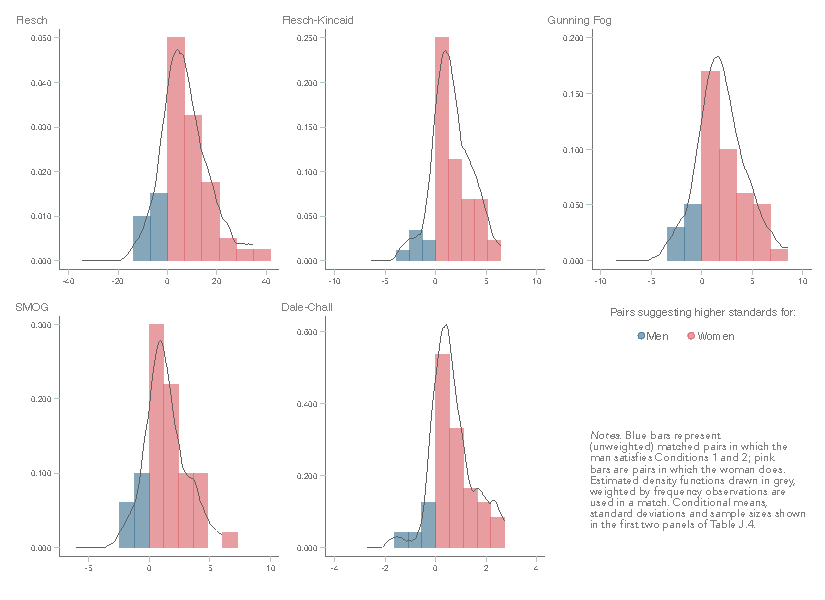
\includegraphics[width=12.3cm]{0-images/generated/Figure-5-jel.pdf}
	}
\end{figure}
\vfill
\clearpage


\subsection{Unadjusted $R_{it}$}
\label{appendixseur}

\autoref{table8_R} and \autoref{figure8_R} replicate the analysis in \autoref{matchingresults} but \autoref{equation14} does not adjust for the ratio of female authors on a paper.


\vfill
\begin{table}[H]
    \footnotesize
    \centering
    \begin{threeparttable}
        \caption{\(D_{ik}\) (\autoref{Corollary1}), without adjusting for the ratio of female authors}
        \label{table8_R}
        \begin{tabular}{p{3cm}S[table-format=3.3]@{}S[table-format=3.3]@{}S[table-format=3.2]@{}S[table-format=4.3]@{}S[table-format=3.3]@{}S[table-format=3.1]@{}S@{}}
            \toprule
            &\multicolumn{3}{c}{{\crcell[b]{Higher standards for\\[-0.1cm]women (\(D_{ik}>0\))}}}&\multicolumn{3}{c}{{\crcell[b]{Higher standards for\\[-0.1cm]men (\(D_{ik}<0\))}}}&{{Mean \(D_{ik}\)}}\\\cmidrule(lr){2-4}\cmidrule(lr){5-7}\cmidrule(lr){8-8}&{{Mean}}&{{S.D.}}&{{\(N\)}}&{{Mean}}&{{S.D.}}&{{\(N\)}}&{{All obs.}}\\
            \midrule
            Flesch                        &        9.67&        7.71&          46&       -5.80&        5.41&          26&        2.47***\\
                                          &            &            &            &            &            &            &      (0.75)   \\
            Flesch Kincaid                &        1.68&        1.41&          51&       -1.24&        1.35&          26&        0.50***\\
                                          &            &            &            &            &            &            &      (0.15)   \\
            Gunning Fog                   &        2.44&        1.80&          42&       -1.53&        1.69&          27&        0.55***\\
                                          &            &            &            &            &            &            &      (0.19)   \\
            SMOG                          &        1.86&        1.39&          40&       -1.05&        1.08&          29&        0.36** \\
                                          &            &            &            &            &            &            &      (0.14)   \\
            Dale-Chall                    &        0.83&        0.66&          50&       -0.62&        0.54&          30&        0.20***\\
                                          &            &            &            &            &            &            &      (0.07)   \\
            \bottomrule
        \end{tabular}
        \begin{tablenotes}
            \tiny
            \item \textit{Notes}. Sample 121 matched pairs. Table displays estimates identical to those in~\autoref{table8_base}, except that \(R_{it}\) is not adjusted for the ratio of female authors on a paper. ***, ** and * statistically significant at 1\%, 5\% and 10\%, respectively.
        \end{tablenotes}
    \end{threeparttable}
\end{table}
\vfill
\begin{figure}[H]
	
	\floatbox{figure}[\FBwidth]
	{
		\caption{Distributions of \(D_{ik}\) (\autoref{Corollary1}), without adjusting for the ratio of female authors}\label{figure8_R}
	}
	{
		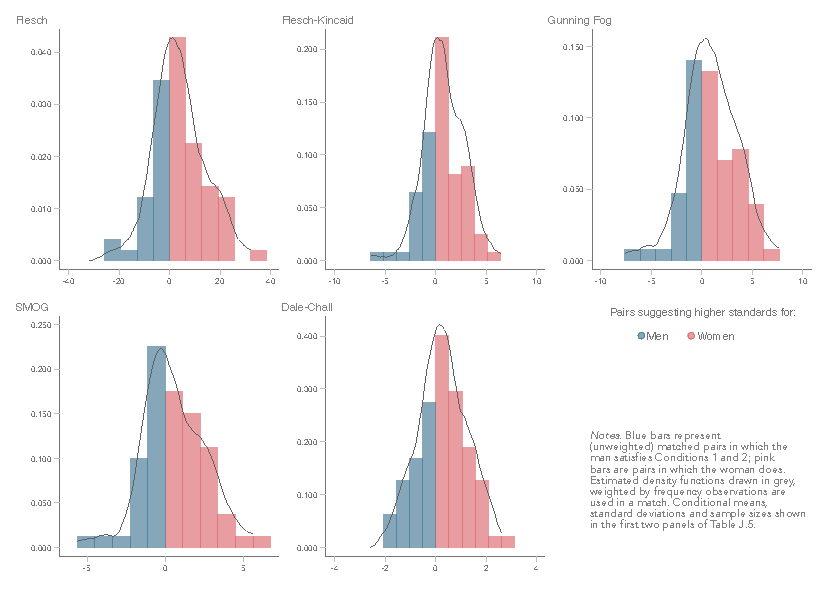
\includegraphics[width=12.3cm]{0-images/generated/Figure-5-R.pdf}
	}
\end{figure}
\vfill
\clearpage


\subsection{Robustness}
\label{appendixmatchinglimitations}

Conclusions drawn in \autoref{matchingresults} are predicated on several strong assumptions. First, all results depend on match accuracy. Post-match co-variates are well balanced (see \aref{appendixmatchingbalance}). They remain well balanced---and similar to the matched population---when restricted to pairs satisfying $D_{ik}\ne0$ (see Appendix M.1 in the \href{http://www.erinhengel.com/research/publishing_female20180828.pdf}{August 2018} version of the paper). To facilitate further scrutiny, \aref{appendixmatchingnames} lists the names of economists in each pair. Matches using alternative variables (\emph{e.g.}, minimum citation counts, mean institutional rank or fraction of articles per primary \emph{JEL} category) and specifications (\emph{e.g.}, propensity score matching) generate similar figures and conclusions.\footnote{See  \citet[][pp. 30--33]{Hengel2017} for propensity score matches from a probit model performed with replacement and using a wider array of co-variates.}

Additionally, authors must be sufficiently experience at $t'$ for Assumptions 4 and 5 in \autoref{Corollary1} to hold. I assume this point occurs at or before authors' third top-four paper. Fifty percent of women with three or more top publications satisfy Conditions 1 \emph{and} 2 when compared to equivalent men. Among them, $D_{ik}$ is far from zero: these women write, on average, 21 percent more clearly than equivalent men with identical experience. I believe it is unlikely that half of all female economists with three top publications---plus many more second-tier publications and substantial experience refereeing and editing themselves---make mistakes of this magnitude.

To generate the counterfactual $\widehat R_{it}$ (\autoref{equation14}), I assume unobserved co-author characteristics do not partially correlate with $\text{female ratio}_{it}$, conditional on $i$'s gender and experience. To test the robustness of this assumption, \autoref{tableH2_Fem100} (\aref{appendixexclusive}) replicates \autoref{tableH2_FemRatio} on exclusively, majority and senior female-authored papers. I have also repeated the analyses shown in \autoref{table8_base} and \autoref{figure8_base} without adjusting for $\text{female ratio}_{it}$ (\aref{appendixseur}) and on subsets of matched pairs in which the woman's $t=1$ and $t=3$ papers are solo- or exclusively female-authored (16), majority female-authored (20) or at least 50 percent female-authored (76). Although sample sizes for the latter three analyses are small, they also find $D_{ik}\ne0$ in about 70--75 percent of matched pairs; most of those (70 percent) indicate higher standards against the female member; the impact across all five scores also averages about 5 percent.

Moreover, experience appears to be the only $t$-varying factor driving within $i$ changes in readability. \autoref{tableH2_FemRatio} and additional analyses in a 2016 version of this paper~\citep[][pp. 23--24]{Hengel2016} show an identical pattern despite controlling for a large array of potential confounders. In a 2017 version, I reconstructed $\widehat R_{it}$ using several $t$-varying factors (number of co-authors, institutional rank, institutional rank of the highest ranked co-author, $t$ for the most experienced co-author, publication year and dummies for each journal)~\citep[][pp. 30, 61]{Hengel2017}; \aref{appendixseujel} adds \emph{JEL} classification codes to \autoref{equation14}. In \autoref{tableH2_Fem100} (\aref{appendixexclusive}), I restrict \autoref{tableH2_FemRatio}'s analysis to solo-authored papers or those co-authored by members of the same sex. In all instances, women's readability is consistently shown to increase with $t$; when comparable results are estimated, they are similar to those presented in \autoref{table8_base} and \autoref{figure8_base}.

Finally, accurate quantification requires that three additional criteria are also met. Assuming higher standards for $i$: (i) $i$'s acceptance rate is no more than $k$'s; (ii) $i$'s draft readability is at least as high as $k$'s; and (iii) $i$'s draft readability at $t=3$ is at least as high as his draft readability at $t=1$. As already discussed in \autoref{mechanismsdescriptive}, (i) rules out the possibility that $i$ is appropriately rewarded (relative to $k$) for writing more clearly. (ii) and (iii) eliminate situations in which women write more clearly during peer review in order to compensate for poorer writing---and consequently higher desk rejection rates---before peer review.

Unfortunately, my data do not perfectly identify acceptance rates nor do I have $t=1$ and $t=3$ draft readability scores for every matched pair. Nevertheless, the data I do have and prior research suggest (i)--(iii) not only hold on average, but do not exert upward bias on my estimate of $D_{ik}$, more generally. First, I reviewed the literature on gender neutrality in journals' acceptance rates in \autoref{mechanismsdescriptive} and \aref{appendixacceptance}; women are not accepted more often than men. Results and conclusions are similar when I attempt to adjust for acceptance rates explicitly by also requiring that $T_{i}\le T_{k}$ for matched pairs in which $i$ is held to higher standards relative to $k$ (see Appendix M.4 in the \href{http://www.erinhengel.com/research/publishing_female20180828.pdf}{August 2018} version of the paper). As shown in \autoref{nber}, women's draft papers are indeed more readable than men's. \autoref{indirecteffect} provides further confirmation. \autoref{figure9} plots the readability of women's and men's draft and published papers over increasing $t$. Women's drafts are more readable than men's drafts at $t=3$ \emph{and} their own drafts at $t=1$.

\clearpage

\section{\autoref{indirecteffect}, supplemental output}
\label{appendixindirecteffect}

\subsection{Experience and review times}
\label{appendixtimeexp}

In \autoref{indirecteffectinterpretation} I find evidence suggesting that inexperienced female economists go through the toughest review, conditional on acceptance. To investigate further, I test the impact of experience on time spent in review by re-estimating \autoref{equation16} on sub-samples of junior ($t=1$) and senior ($t>1$) authors.\footnote{Three notes on estimation. First, in \autoref{quantification}, I define ``experienced'' as $t=3$. However, most female-authored papers published in \emph{Econometrica} and \emph{REStud} are by women with no (or only one) previous top publication; only 24 have two or more previous papers and were the most senior co-author on a $t>2$ paper. Second, to eliminate confounding by more senior co-authors, I restrict the sample to the senior authors on a paper (\emph{i.e.}, authors satisfying $\text{max. } t=t$). (Including these observations does not substantially impact results or conclusions.) Third, because the sample includes data from \emph{REStud}, readability, motherhood and childbirth controls are not included. See the \href{http://www.erinhengel.com/research/publishing_female20180828.pdf}{August 2018} version of this paper for results that control for these factors (based on data from \emph{Econometrica} alone).} Results are displayed in \autoref{figure11}. They suggest papers by junior women do indeed take longer in review; the gender gap is significantly smaller---albeit still positive---for senior women.


\begin{figure}[H]
	
	\floatbox{figure}[\FBwidth]
	{
		\caption{The impact of experience on women's review times}\label{figure11}
	}
	{
		\includegraphics[trim=0cm 2.55cm 0cm 2.3cm, clip, width=0.95\linewidth]{0-images/generated/{Figure-K.1}.pdf}
		\floatfoot{\tiny \textit{Notes}. Sample restricted to senior authors on a paper (5,007 observations). Blue dots are the coefficients on female ratio (papers with fewer than 50 percent female authors are classified as male, see~\autoref{gender}) corresponding to separate FGLS estimations of~\autoref{equation16} on junior ($t=1$) and senior ($t>1$) authors, respectively. The yellow dot is their difference. Vertical grey lines correspond to 90 percent confidence intervals. Regressions weighted by $1/N_j$.}
	}
\end{figure}
\clearpage

\section{Alternative program for calculating readability scores}
\label{appendixalternativereadability}

In this section, I replicate \autoref{table3_FemRatio}, \autoref{table6_FemRatio}, \autoref{tableH2_FemRatio} and \autoref{table4_FemRatio} using readability scores generated by the \href{https://github.com/trinker/readability}{R \texttt{readability} package}, an alternative program for calculating Flesch-Kincaid, Gunning Fog and SMOG readability scores. Replications for other tables and figures presented in the paper are not shown, but will be made available on request.

\texttt{Textatistic} and \texttt{readability} employ different strategies to adapt the scores to automated calculation---\emph{e.g.}, \texttt{readability} counts semi-colons and dashes as sentence-ending terminations; \texttt{Textatistic} does not.\footnote{Readability scores were originally developed to be calculated by hand. Automating their calculation requires slightly adapting the algorithms. For example, all five scores define sentences as grammatically independent units of thoughts---\emph{e.g.}, two independent clauses connected by a dash or semi-colon count as two separate sentences. Unfortunately, semi-colons and dashes are frequently used in other ways and it is difficult to programmatically distinguish between contexts.} Results appear robust to these (and other) small discrepancies: coefficients are similar to those presented in the body of the paper.


\begin{table}[H]
    \footnotesize
    \centering
    \begin{threeparttable}
        \caption{\autoref{table3_FemRatio}, alternative program for calculating readability}
        \label{table3_R}
        \begin{tabular}{p{2cm}S@{}S@{}S@{}S@{}S@{}S@{}S@{}S@{}S@{}}
            \toprule
            &\multicolumn{5}{c}{1950--2015}&\multicolumn{4}{c}{1990--2015}\\\cmidrule(lr){2-6}\cmidrule(lr){7-10}&{(1)}&{(2)}&{(3)}&{(4)}&{(5)}&{(6)}&{(7)}&{(8)}&{(9)}\\
            \midrule
            \mrow{3cm}{Flesch-Kincaid}    &        0.23*  &        0.23*  &        0.23*  &        0.26** &        0.28** &        0.34** &        0.37** &        0.35** &        0.49***\\
                                          &      (0.13)   &      (0.13)   &      (0.12)   &      (0.13)   &      (0.13)   &      (0.15)   &      (0.14)   &      (0.15)   &      (0.16)   \\
            \mrow{3cm}{Gunning Fog}       &        0.37***&        0.37***&        0.38***&        0.42***&        0.43***&        0.45***&        0.45***&        0.46***&        0.54***\\
                                          &      (0.13)   &      (0.13)   &      (0.13)   &      (0.14)   &      (0.14)   &      (0.15)   &      (0.14)   &      (0.16)   &      (0.18)   \\
            \mrow{3cm}{SMOG}              &        0.24** &        0.25** &        0.25** &        0.27***&        0.29***&        0.30** &        0.30***&        0.31** &        0.36***\\
                                          &      (0.10)   &      (0.10)   &      (0.10)   &      (0.10)   &      (0.10)   &      (0.11)   &      (0.10)   &      (0.12)   &      (0.13)   \\
            \midrule
            No. obs.                      &       9,117   &       9,117   &       9,117   &       9,117   &       9,117   &       5,211   &       5,211   &       5,211   &       5,774   \\
            \midrule
            Editor               &           {\ding{51}}   &           {\ding{51}}   &           {\ding{51}}   &           {\ding{51}}   &           {\ding{51}}   &           {\ding{51}}   &           {\ding{51}}   &           {\ding{51}}   &           {\ding{51}}   \\
            Blind                         &           {\ding{51}}   &           {\ding{51}}   &           {\ding{51}}   &           {\ding{51}}   &           {\ding{51}}   &           {\ding{51}}   &           {\ding{51}}   &           {\ding{51}}   &           {\ding{51}}   \\
            Journal                       &           {\ding{51}}   &           {\ding{51}}   &               &               &               &               &               &               &               \\
            Year                          &               &           {\ding{51}}   &               &               &               &               &               &               &               \\
            Journal\(\times\)Year                  &               &               &           {\ding{51}}   &           {\ding{51}}   &           {\ding{51}}   &           {\ding{51}}   &           {\ding{51}}   &           {\ding{51}}   &           {\ding{51}}   \\
            \(N_j\)                       &               &               &               &           {\ding{51}}   &           {\ding{51}}   &           {\ding{51}}   &           {\ding{51}}   &           {\ding{51}}   &           {\ding{51}}   \\
            Institution                   &               &               &               &           {\ding{51}}   &           {\ding{51}}   &           {\ding{51}}   &           {\ding{51}}   &           {\ding{51}}   &           {\ding{51}}   \\
            Quality                       &               &               &               &               &          {\(\text{\ding{51}}^1\)}   &          {\(\text{\ding{51}}^1\)}   &          {\(\text{\ding{51}}^1\)}   &          {\(\text{\ding{51}}^1\)}   &          {\(\text{\ding{51}}^1\)}   \\
            Native speaker                &               &               &               &               &           {\ding{51}}   &           {\ding{51}}   &           {\ding{51}}   &           {\ding{51}}   &           {\ding{51}}   \\
            \textit{JEL} (primary)        &               &               &               &               &               &               &           {\ding{51}}   &               &               \\
            Theory/empirical              &               &               &               &               &               &               &               &           {\ding{51}}   &               \\
            \textit{JEL} (tertiary)       &               &               &               &               &               &               &               &               &           {\ding{51}}   \\
            \bottomrule
        \end{tabular}
        \begin{tablenotes}
            \tiny
            \item \textit{Notes}. Estimates are identical to those in \autoref{table3_FemRatio}, except readability scores were calculated using the R \texttt{readability} program. ***, ** and * statistically significant at 1\%, 5\% and 10\%, respectively.
        \end{tablenotes}
    \end{threeparttable}
\end{table}
\clearpage
\begin{sidewaystable}
    \footnotesize
    \centering
    \begin{threeparttable}
        \caption{\autoref{table6_FemRatio}, alternative program for calculating readability}
        \label{table6_R}
        \begin{tabular}{p{3cm}S@{}S@{}S@{}S@{}S@{}S@{}S@{}S@{}S@{}S@{}S@{}}
            \toprule
            &\multicolumn{3}{c}{{OLS (score)}}&\multicolumn{2}{c}{{OLS ($\Delta$ in score)}}&\multicolumn{6}{c}{{FGLS (score)}}\\\cmidrule(lr){2-4}\cmidrule(lr){5-6}\cmidrule(lr){7-12}&&&&&&\multicolumn{2}{c}{{Working paper}}&\multicolumn{2}{c}{{Published paper}}&\multicolumn{2}{c}{{Difference}}\\\cmidrule(lr){7-8}\cmidrule(lr){9-10}\cmidrule(lr){11-12}&{\(R_{jW}\)}&{\crcell[b]{Female\\[-0.1cm]ratio}}&{\crcell[b]{Blind$\times$\\[-0.1cm]fem. ratio}}&{\crcell[b]{Female\\[-0.1cm]ratio}}&{\crcell[b]{Blind$\times$\\[-0.1cm]fem. ratio}}&{\crcell[b]{Female\\[-0.1cm]ratio}}&{\crcell[b]{Blind$\times$\\[-0.1cm]fem. ratio}}&{\crcell[b]{Female\\[-0.1cm]ratio}}&{\crcell[b]{Blind$\times$\\[-0.1cm]fem. ratio}}&{\crcell[b]{Female\\[-0.1cm]ratio}}&{\crcell[b]{Blind$\times$\\[-0.1cm]fem. ratio}}\\
            \midrule
            Flesch-Kincaid                &        0.74***&        0.55***&       -1.13   &        0.47** &       -0.94   &        0.30   &       -0.76   &        0.77***&       -1.69***&        0.47** &       -0.94   \\
                                          &      (0.03)   &      (0.20)   &      (0.74)   &      (0.21)   &      (0.62)   &      (0.25)   &      (0.77)   &      (0.28)   &      (0.44)   &      (0.20)   &      (0.61)   \\
            Gunning Fog                   &        0.77***&        0.56***&       -1.40   &        0.46** &       -1.21   &        0.42   &       -0.84   &        0.89***&       -2.05***&        0.46** &       -1.21   \\
                                          &      (0.03)   &      (0.21)   &      (0.90)   &      (0.21)   &      (0.76)   &      (0.27)   &      (0.95)   &      (0.26)   &      (0.64)   &      (0.21)   &      (0.75)   \\
            SMOG                          &        0.77***&        0.40** &       -1.01   &        0.33** &       -0.86   &        0.27   &       -0.63   &        0.61***&       -1.50***&        0.33** &       -0.86   \\
                                          &      (0.02)   &      (0.16)   &      (0.65)   &      (0.15)   &      (0.55)   &      (0.18)   &      (0.71)   &      (0.18)   &      (0.49)   &      (0.15)   &      (0.54)   \\
            \midrule
            No. observations              &               &       1,988   &               &       1,988   &               &       1,988   &               &       1,988   &               &       1,988   &               \\
            \midrule
            Editor effects       &               &           {\ding{51}}   &               &           {\ding{51}}   &               &           {\ding{51}}   &               &           {\ding{51}}   &               &               &               \\
            Journal\(\times\)Year effects          &               &           {\ding{51}}   &               &           {\ding{51}}   &               &           {\ding{51}}   &               &           {\ding{51}}   &               &               &               \\
            \(N_j\)                       &               &           {\ding{51}}   &               &           {\ding{51}}   &               &           {\ding{51}}   &               &           {\ding{51}}   &               &               &               \\
            Quality controls              &               &          {\(\text{\ding{51}}^2\)}   &               &          {\(\text{\ding{51}}^2\)}   &               &          {\(\text{\ding{51}}^2\)}   &               &          {\(\text{\ding{51}}^2\)}   &               &               &               \\
            Native speaker                &               &           {\ding{51}}   &               &           {\ding{51}}   &               &           {\ding{51}}   &               &           {\ding{51}}   &               &               &               \\
            Theory/emp. effects           &               &           {\ding{51}}   &               &           {\ding{51}}   &               &           {\ding{51}}   &               &           {\ding{51}}   &               &               &               \\
            \bottomrule
        \end{tabular}
        \begin{tablenotes}
            \tiny
            \item \textit{Notes}. Estimates are identical to those in \autoref{table6_FemRatio}, except readability scores were calculated using the R \texttt{readability} program. ***, ** and * statistically significant at 1\%, 5\% and 10\%, respectively.
        \end{tablenotes}
    \end{threeparttable}

\end{sidewaystable}

\clearpage
\begin{table}
    \footnotesize
    \centering
    \begin{threeparttable}
        \caption{\autoref{tableH2_FemRatio}, alternative program for calculating readability}
        \label{tableH2_R}
        \begin{tabular}{p{3cm}S@{}S@{}S@{}S@{}S@{}S@{}S@{}}
            \toprule
            &{\(t=1\)}&{\(t=2\)}&{\(t=3\)}&{\(t=4\text{--}5\)}&{\(t\ge6\)}&{All}\\
            \midrule
            Flesch-Kincaid                &        0.08   &        0.28   &        1.12***&        0.62   &        0.55   &        0.28*  \\
                                          &      (0.18)   &      (0.27)   &      (0.26)   &      (0.49)   &      (0.39)   &      (0.17)   \\
            Gunning Fog                   &        0.25   &        0.37   &        1.41***&        0.84   &        0.63   &        0.50***\\
                                          &      (0.20)   &      (0.27)   &      (0.35)   &      (0.55)   &      (0.45)   &      (0.19)   \\
            SMOG                          &        0.17   &        0.28   &        0.92***&        0.56   &        0.41   &        0.34***\\
                                          &      (0.15)   &      (0.20)   &      (0.23)   &      (0.40)   &      (0.31)   &      (0.13)   \\
            \midrule
            No. observations              &       6,874   &       2,827   &       1,675   &       1,906   &       2,773   &      12,008   \\
            \midrule
            Editor effects       &           {\ding{51}}   &           {\ding{51}}   &           {\ding{51}}   &           {\ding{51}}   &           {\ding{51}}   &           {\ding{51}}   \\
            Blind review                  &           {\ding{51}}   &           {\ding{51}}   &           {\ding{51}}   &           {\ding{51}}   &           {\ding{51}}   &           {\ding{51}}   \\
            Journal\(\times\)Year effects          &           {\ding{51}}   &           {\ding{51}}   &           {\ding{51}}   &           {\ding{51}}   &           {\ding{51}}   &           {\ding{51}}   \\
            \(N_j\)                       &           {\ding{51}}   &           {\ding{51}}   &           {\ding{51}}   &           {\ding{51}}   &           {\ding{51}}   &           {\ding{51}}   \\
            Institution effects           &           {\ding{51}}   &           {\ding{51}}   &           {\ding{51}}   &           {\ding{51}}   &           {\ding{51}}   &           {\ding{51}}   \\
            Quality controls              &          {\(\text{\ding{51}}^3\)}   &          {\(\text{\ding{51}}^3\)}   &          {\(\text{\ding{51}}^3\)}   &          {\(\text{\ding{51}}^3\)}   &          {\(\text{\ding{51}}^3\)}   &          {\(\text{\ding{51}}^1\)}   \\
            Native speaker                &           {\ding{51}}   &           {\ding{51}}   &           {\ding{51}}   &           {\ding{51}}   &           {\ding{51}}   &           {\ding{51}}   \\
            \bottomrule
        \end{tabular}
        \begin{tablenotes}
            \tiny
            \item \textit{Notes}. Estimates are identical to those in \autoref{tableH2_FemRatio}, except readability scores were calculated using the R \texttt{readability} program. ***, ** and * statistically significant at 1\%, 5\% and 10\%, respectively.
        \end{tablenotes}
    \end{threeparttable}
\end{table}
\clearpage
\begin{table}
    \footnotesize
    \centering
    \begin{threeparttable}
        \caption{\autoref{table4_FemRatio}, alternative program for calculating readability}
        \label{table4_R}
        \begin{tabular}{p{4cm}S@{}S@{}S@{}}
            \toprule
            &{\crcell[b]{Flesch-\\[-0.1cm]Kincaid}}&{\crcell[b]{Gunning\\[-0.1cm]Fog}}&{SMOG}\\
            \midrule
            \mrow{4cm}{Female ratio for women (\(\beta_1\))}&        0.33   &        0.48** &        0.30*  \\
                                          &      (0.21)   &      (0.24)   &      (0.17)   \\
            \mrow{4cm}{Female ratio for men (\(\beta_1+\beta_2\))}&        0.38   &        0.50   &        0.32   \\
                                          &      (0.30)   &      (0.34)   &      (0.24)   \\
            \mrow{4cm}{Female ratio\(\times\)male (\(\beta_2\))}&        0.05   &        0.02   &        0.02   \\
                                          &      (0.35)   &      (0.40)   &      (0.28)   \\
            \mrow{4cm}{Lagged score (\(\beta_0\))}&        0.05** &        0.04*  &        0.04*  \\
                                          &      (0.02)   &      (0.02)   &      (0.02)   \\
            \midrule
            No. observations     &       9,181   &       9,181   &       9,181   \\
            \mcol{\textit{Tests of instrument validity}} \\
            \quad Hansen test (\(p\)-value)&       0.841   &       0.735   &       0.734   \\
            \quad Sargan test (\(p\)-value)&       0.156   &       0.213   &       0.112   \\
            \mcol{\textit{\(z\)-test for no serial correlation}} \\
            \quad Order 1&     -12.478   &     -13.245   &     -16.851   \\
            \quad Order 2                 &       0.084   &       0.586   &       0.464   \\
            \midrule
            Editor effects       &           {\ding{51}}   &           {\ding{51}}   &           {\ding{51}}   \\
            Blind review                  &           {\ding{51}}   &           {\ding{51}}   &           {\ding{51}}   \\
            Journal effects               &           {\ding{51}}   &           {\ding{51}}   &           {\ding{51}}   \\
            \(N_j\)                       &           {\ding{51}}   &           {\ding{51}}   &           {\ding{51}}   \\
            Institution effects           &           {\ding{51}}   &           {\ding{51}}   &           {\ding{51}}   \\
            Quality controls              &          {\(\text{\ding{51}}^2\)}   &          {\(\text{\ding{51}}^2\)}   &          {\(\text{\ding{51}}^2\)}   \\
            Native speaker                &           {\ding{51}}   &           {\ding{51}}   &           {\ding{51}}   \\
            \bottomrule
        \end{tabular}
        \begin{tablenotes}
            \tiny
            \item \textit{Notes}. Estimates are identical to those in \autoref{table4_FemRatio}, except readability scores were calculated using the R \texttt{readability} program. ***, ** and * statistically significant at 1\%, 5\% and 10\%, respectively.
        \end{tablenotes}
    \end{threeparttable}
\end{table}
\clearpage


\section{Alternative proxies for article gender}
\label{appendixalternativemeasure}

In this appendix, I replicate \autoref{table3_FemRatio}, \autoref{table6_FemRatio}, \autoref{table10_FemRatio}, \autoref{table11_FemRatio}, \autoref{tableH2_FemRatio} and \autoref{table4_FemRatio} using the alternative proxies for article gender summarised in \autoref{SampleSummaries}.

\begin{sidewaystable}[H]
	\footnotesize
	\centering
	\begin{threeparttable}
		\caption{Summary of alternative proxies for female-authored papers}
		\label{SampleSummaries}
		\begin{tabular}{L{3cm}L{2cm}L{6cm}L{6cm}L{5cm}}
			\toprule
			Proxy for female-authorship&Appendix&Description&Sample restrictions&Additional notes\\
			\midrule
			Female solo-authored papers&\aref{appendixsolo}&Article gender is represented by a dummy variable equal to 1 if the paper is solo-authored by a woman and 0 if it is solo-authored by a man.&Co-authored papers are excluded in all tables except~\autoref{table4_FemSolo} where they are classified as male-authored papers in order to increase within-author variation.&\\
			Senior-female authored papers&\aref{appendixsenior}&Article gender is represented by the interaction between female ratio and a dummy variable equal to 1 if a female author had at least as many top-five papers as her co-authors at the time the paper was published.&Mixed-gendered papers without a senior female co-author are excluded in all tables except~\autoref{table4_FemSenior} where they are classified as male-authored papers in order to increase within-author variation.&\\
			Majority female-authored papers&\aref{appendixmajority}&Article gender is represented by a dummy variable equal to 1 if at least half of all authors are female.&Mixed-gendered papers with a strict minority of female authors are excluded in all tables except~\autoref{table4_Fem50} where they are classified as male-authored papers in order to increase within-author variation.&\\
			Papers with at least one female author&\aref{appendixminority}&Article gender is represented by a dummy variable equal to 1 if at least one author on a paper is female.&&\\
			Exclusively female-authored papers&\aref{appendixexclusive}&Article gender is represented by a dummy variable equal to 1 if all authors on a paper are female.&Mixed-gendered papers are excluded in all tables except~\autoref{table4_Fem100} where they are classified as male-authored papers in order to increase within-author variation.&\\
			Senior female-authored papers, sample of less experienced authors&\aref{appendixjunior}&Article gender is represented by the interaction between female ratio and a dummy variable equal to 1 if a female author had at least as many top-five papers as her co-authors at the time the paper was published.&Mixed-gendered papers without a senior female co-author and all papers by authors with more than three top-five papers are excluded in all tables.&\autoref{tableH2_FemRatio} and \autoref{table4_FemRatio} are not estimated. NBER has released very few working papers in which a woman with only one or two top papers is the most senior author on a paper with more than one author. Results in \autoref{table6_FemJunior} should therefore be interpreted with caution.\\
			\bottomrule
		\end{tabular}
	\end{threeparttable}
\end{sidewaystable}

\subsection{Solo-authored}
\label{appendixsolo}


\begin{vplace}[0.7]
\begin{table}[H]
    \footnotesize
    \centering
    \begin{threeparttable}
        \caption{\autoref{table3_FemRatio}, solo-authored papers}
        \label{table3_FemSolo}
        \begin{tabular}{p{2cm}S@{}S@{}S@{}S@{}S@{}S@{}S@{}S@{}S@{}}
            \toprule
            &\multicolumn{5}{c}{1950--2015}&\multicolumn{4}{c}{1990--2015}\\\cmidrule(lr){2-6}\cmidrule(lr){7-10}&{(1)}&{(2)}&{(3)}&{(4)}&{(5)}&{(6)}&{(7)}&{(8)}&{(9)}\\
            \midrule
            \mrow{3cm}{Flesch}            &        0.37   &        0.41   &        0.25   &        0.25   &        0.46   &        0.52   &        0.46   &        0.59   &        0.62   \\
                                          &      (0.74)   &      (0.75)   &      (0.74)   &      (0.74)   &      (0.75)   &      (0.85)   &      (0.81)   &      (0.88)   &      (1.75)   \\
            \mrow{3cm}{Flesch-Kincaid}    &        0.13   &        0.13   &        0.11   &        0.12   &        0.09   &        0.27   &        0.27   &        0.28   &        0.10   \\
                                          &      (0.17)   &      (0.17)   &      (0.16)   &      (0.16)   &      (0.17)   &      (0.17)   &      (0.17)   &      (0.17)   &      (0.31)   \\
            \mrow{3cm}{Gunning Fog}       &        0.21   &        0.22   &        0.19   &        0.21   &        0.18   &        0.40** &        0.36*  &        0.42** &        0.20   \\
                                          &      (0.19)   &      (0.19)   &      (0.18)   &      (0.18)   &      (0.18)   &      (0.18)   &      (0.18)   &      (0.19)   &      (0.36)   \\
            \mrow{3cm}{SMOG}              &        0.13   &        0.15   &        0.13   &        0.14   &        0.14   &        0.26*  &        0.22*  &        0.28*  &        0.16   \\
                                          &      (0.14)   &      (0.14)   &      (0.13)   &      (0.13)   &      (0.13)   &      (0.14)   &      (0.13)   &      (0.14)   &      (0.26)   \\
            \mrow{3cm}{Dale-Chall}        &       -0.01   &       -0.01   &       -0.02   &       -0.02   &       -0.01   &        0.05   &        0.06   &        0.06   &        0.10   \\
                                          &      (0.06)   &      (0.07)   &      (0.07)   &      (0.07)   &      (0.07)   &      (0.08)   &      (0.07)   &      (0.08)   &      (0.12)   \\
            \midrule
            No. obs.                      &       4,014   &       4,014   &       4,014   &       4,014   &       4,014   &       1,540   &       1,540   &       1,540   &       1,666   \\
            \midrule
            Editor               &           {\ding{51}}   &           {\ding{51}}   &           {\ding{51}}   &           {\ding{51}}   &           {\ding{51}}   &           {\ding{51}}   &           {\ding{51}}   &           {\ding{51}}   &           {\ding{51}}   \\
            Blind                         &           {\ding{51}}   &           {\ding{51}}   &           {\ding{51}}   &           {\ding{51}}   &           {\ding{51}}   &           {\ding{51}}   &           {\ding{51}}   &           {\ding{51}}   &           {\ding{51}}   \\
            Journal                       &           {\ding{51}}   &           {\ding{51}}   &               &               &               &               &               &               &               \\
            Year                          &               &           {\ding{51}}   &               &               &               &               &               &               &               \\
            Journal\(\times\)Year                  &               &               &           {\ding{51}}   &           {\ding{51}}   &           {\ding{51}}   &           {\ding{51}}   &           {\ding{51}}   &           {\ding{51}}   &           {\ding{51}}   \\
            \(N_j\)                       &               &               &               &           {\ding{51}}   &           {\ding{51}}   &           {\ding{51}}   &           {\ding{51}}   &           {\ding{51}}   &           {\ding{51}}   \\
            Institution                   &               &               &               &           {\ding{51}}   &           {\ding{51}}   &           {\ding{51}}   &           {\ding{51}}   &           {\ding{51}}   &           {\ding{51}}   \\
            Quality                       &               &               &               &               &          {\(\text{\ding{51}}^1\)}   &          {\(\text{\ding{51}}^1\)}   &          {\(\text{\ding{51}}^1\)}   &          {\(\text{\ding{51}}^1\)}   &          {\(\text{\ding{51}}^1\)}   \\
            Native speaker                &               &               &               &               &           {\ding{51}}   &           {\ding{51}}   &           {\ding{51}}   &           {\ding{51}}   &           {\ding{51}}   \\
            \textit{JEL} (primary)        &               &               &               &               &               &               &           {\ding{51}}   &               &               \\
            Theory/empirical              &               &               &               &               &               &               &               &           {\ding{51}}   &               \\
            \textit{JEL} (tertiary)       &               &               &               &               &               &               &               &               &           {\ding{51}}   \\
            \bottomrule
        \end{tabular}
        \begin{tablenotes}
            \tiny
            \item \textit{Notes}. Estimates are identical to those in \autoref{table3_FemRatio}, except that female ratio has been replaced with a dummy variable equal to 1 if the paper is solo-authored by a woman and 0 if it is solo-authored by a man. (Co-authored papers are excluded.) ***, ** and * statistically significant at 1\%, 5\% and 10\%, respectively.
        \end{tablenotes}
    \end{threeparttable}
\end{table}
\end{vplace}
\clearpage
\begin{sidewaystable}
    \footnotesize
    \centering
    \begin{threeparttable}
        \caption{\autoref{table6_FemRatio}, solo-authored papers}
        \label{table6_FemSolo}
        \begin{tabular}{p{3cm}S@{}S@{}S@{}S@{}S@{}S@{}S@{}S@{}S@{}S@{}S@{}}
            \toprule
            &\multicolumn{3}{c}{{OLS (score)}}&\multicolumn{2}{c}{{OLS ($\Delta$ in score)}}&\multicolumn{6}{c}{{FGLS (score)}}\\\cmidrule(lr){2-4}\cmidrule(lr){5-6}\cmidrule(lr){7-12}&&&&&&\multicolumn{2}{c}{{Working paper}}&\multicolumn{2}{c}{{Published paper}}&\multicolumn{2}{c}{{Difference}}\\\cmidrule(lr){7-8}\cmidrule(lr){9-10}\cmidrule(lr){11-12}&{\(R_{jW}\)}&{\crcell[b]{Female}}&{\crcell[b]{Blind$\times$\\[-0.1cm]female}}&{\crcell[b]{Female}}&{\crcell[b]{Blind$\times$\\[-0.1cm]female}}&{\crcell[b]{Female}}&{\crcell[b]{Blind$\times$\\[-0.1cm]female}}&{\crcell[b]{Female}}&{\crcell[b]{Blind$\times$\\[-0.1cm]female}}&{\crcell[b]{Female}}&{\crcell[b]{Blind$\times$\\[-0.1cm]female}}\\
            \midrule
            Flesch                        &        0.79***&        1.34   &       -4.31   &        1.19   &       -4.96   &        0.74   &        3.13   &        1.93   &       -1.83   &        1.19   &       -4.96   \\
                                          &      (0.08)   &      (1.43)   &      (7.53)   &      (1.28)   &      (4.91)   &      (2.10)   &      (4.46)   &      (2.40)   &      (4.10)   &      (1.19)   &      (4.56)   \\
            Flesch-Kincaid                &        0.76***&        0.66   &       -1.81   &        0.62   &       -1.78   &        0.17   &       -0.10   &        0.78   &       -1.88** &        0.62*  &       -1.78*  \\
                                          &      (0.14)   &      (0.50)   &      (1.34)   &      (0.37)   &      (1.14)   &      (0.42)   &      (1.04)   &      (0.57)   &      (0.94)   &      (0.35)   &      (1.06)   \\
            Gunning Fog                   &        0.73***&        0.71   &       -2.09   &        0.67   &       -2.19*  &        0.18   &        0.36   &        0.84   &       -1.83*  &        0.67*  &       -2.19*  \\
                                          &      (0.11)   &      (0.55)   &      (1.50)   &      (0.42)   &      (1.27)   &      (0.46)   &      (1.17)   &      (0.62)   &      (0.95)   &      (0.39)   &      (1.18)   \\
            SMOG                          &        0.74***&        0.35   &       -1.32   &        0.31   &       -1.41   &        0.15   &        0.33   &        0.46   &       -1.08*  &        0.31   &       -1.41*  \\
                                          &      (0.06)   &      (0.30)   &      (1.02)   &      (0.27)   &      (0.86)   &      (0.34)   &      (0.80)   &      (0.39)   &      (0.58)   &      (0.25)   &      (0.80)   \\
            Dale-Chall                    &        0.86***&        0.19   &       -0.43   &        0.16   &       -0.46   &        0.17   &        0.18   &        0.34** &       -0.28   &        0.16   &       -0.46*  \\
                                          &      (0.04)   &      (0.15)   &      (0.52)   &      (0.16)   &      (0.28)   &      (0.15)   &      (0.36)   &      (0.16)   &      (0.38)   &      (0.15)   &      (0.26)   \\
            \midrule
            No. observations              &               &         434   &               &         434   &               &         434   &               &         434   &               &         434   &               \\
            \midrule
            Editor effects       &               &           {\ding{51}}   &               &           {\ding{51}}   &               &           {\ding{51}}   &               &           {\ding{51}}   &               &               &               \\
            Journal\(\times\)Year effects          &               &           {\ding{51}}   &               &           {\ding{51}}   &               &           {\ding{51}}   &               &           {\ding{51}}   &               &               &               \\
            \(N_j\)                       &               &           {\ding{51}}   &               &           {\ding{51}}   &               &           {\ding{51}}   &               &           {\ding{51}}   &               &               &               \\
            Quality controls              &               &          {\(\text{\ding{51}}^2\)}   &               &          {\(\text{\ding{51}}^2\)}   &               &          {\(\text{\ding{51}}^2\)}   &               &          {\(\text{\ding{51}}^2\)}   &               &               &               \\
            Native speaker                &               &           {\ding{51}}   &               &           {\ding{51}}   &               &           {\ding{51}}   &               &           {\ding{51}}   &               &               &               \\
            Theory/emp. effects           &               &           {\ding{51}}   &               &           {\ding{51}}   &               &           {\ding{51}}   &               &           {\ding{51}}   &               &               &               \\
            \bottomrule
        \end{tabular}
        \begin{tablenotes}
            \tiny
            \item \textit{Notes}. Estimates are identical to those in \autoref{table6_FemRatio}, except that female ratio has been replaced with a dummy variable equal to 1 if the paper is solo-authored by a woman and 0 if it is solo-authored by a man. (Co-authored papers are excluded.) ***, ** and * statistically significant at 1\%, 5\% and 10\%, respectively.
        \end{tablenotes}
    \end{threeparttable}

\end{sidewaystable}

\clearpage
\begin{table}
    \begin{adjustwidth}{-0.085cm}{}
    \footnotesize
    \centering
    \begin{threeparttable}
        \caption{\autoref{table10_FemRatio}, solo-authored papers}
        \label{table10_FemSolo}
        \sisetup{round-precision=3,table-format=3.4}
        \begin{tabular}{p{2.64cm}SSSSSSS}
            \toprule
            &\multicolumn{5}{c}{1970--2015}&\multicolumn{2}{c}{1990--2015}\\\cmidrule(lr){2-6}\cmidrule(lr){7-8}&{(1)}&{(2)}&{(3)}&{(4)}&{(5)}&{(6)}&{(7)}\\
            \midrule
            Solo female                   &       7.313** &      10.433** &      10.220** &       8.068** &      10.354** &      13.216** &      14.608** \\
                                          &     (2.964)   &     (4.088)   &     (4.069)   &     (3.602)   &     (4.068)   &     (6.035)   &     (5.767)   \\
            Max. \(t\)                    &      -0.311***&      -0.309***&      -0.308***&      -0.312***&      -0.305***&      -0.284***&      -0.279** \\
                                          &     (0.080)   &     (0.079)   &     (0.080)   &     (0.081)   &     (0.079)   &     (0.102)   &     (0.109)   \\
            No. pages                     &       0.198***&       0.196***&       0.193***&       0.197***&       0.192***&       0.267***&       0.264***\\
                                          &     (0.041)   &     (0.041)   &     (0.040)   &     (0.041)   &     (0.040)   &     (0.063)   &     (0.066)   \\
            Order                         &       0.175** &       0.179** &       0.170** &       0.172** &       0.173** &       0.610*  &       0.479   \\
                                          &     (0.082)   &     (0.082)   &     (0.081)   &     (0.081)   &     (0.081)   &     (0.307)   &     (0.299)   \\
            No. citations (asinh)         &      -0.693***&      -0.745***&      -0.702***&      -0.686***&      -0.724***&      -1.150*  &      -1.065*  \\
                                          &     (0.180)   &     (0.174)   &     (0.178)   &     (0.182)   &     (0.177)   &     (0.584)   &     (0.535)   \\
            Flesch                        &      -0.009   &      -0.009   &      -0.008   &      -0.009   &      -0.006   &      -0.001   &       0.008   \\
                                          &     (0.022)   &     (0.022)   &     (0.022)   &     (0.022)   &     (0.023)   &     (0.058)   &     (0.063)   \\
            Theory                        &       1.859   &       1.807   &       1.751   &       1.819   &       1.772   &       2.143   &      -0.305   \\
                                          &     (1.312)   &     (1.338)   &     (1.347)   &     (1.331)   &     (1.344)   &     (1.441)   &     (2.554)   \\
            Empirical                     &      -8.025** &      -7.865*  &      -8.537** &      -8.113** &      -8.661** &      -9.072** &     -10.639** \\
                                          &     (3.325)   &     (4.064)   &     (3.410)   &     (3.303)   &     (3.474)   &     (3.854)   &     (4.146)   \\
            Other                         &       1.451   &       1.272   &       1.452   &       1.465   &       1.421   &       1.831   &       2.064   \\
                                          &     (1.918)   &     (1.863)   &     (1.889)   &     (1.904)   &     (1.916)   &     (2.073)   &     (3.000)   \\
            Mother                        &               &               &      -9.050** &               &     -14.724***&     -31.324***&     -32.020***\\
                                          &               &               &     (4.455)   &               &     (5.315)   &     (9.349)   &     (9.563)   \\
            Birth                         &               &               &               &      -3.945   &       8.818*  &      26.982***&      28.360***\\
                                          &               &               &               &     (4.821)   &     (5.044)   &     (6.856)   &     (7.206)   \\
            Constant                      &      13.932***&      14.287***&      14.045***&      13.947***&      14.084***&      16.312***&      17.769***\\
                                          &     (2.554)   &     (2.453)   &     (2.515)   &     (2.543)   &     (2.519)   &     (5.577)   &     (5.379)   \\
            \midrule
            \(R^2\)                       &       0.344   &       0.349   &       0.348   &       0.345   &       0.349   &       0.227   &       0.260   \\
            No. observations              &       1,224   &       1,210   &       1,224   &       1,224   &       1,224   &         418   &         418   \\
            \midrule
            Editor effects       &           {\ding{51}}   &           {\ding{51}}   &           {\ding{51}}   &           {\ding{51}}   &           {\ding{51}}   &           {\ding{51}}   &           {\ding{51}}   \\
            Year effects                  &           {\ding{51}}   &           {\ding{51}}   &           {\ding{51}}   &           {\ding{51}}   &           {\ding{51}}   &           {\ding{51}}   &           {\ding{51}}   \\
            Institution effects           &           {\ding{51}}   &           {\ding{51}}   &           {\ding{51}}   &           {\ding{51}}   &           {\ding{51}}   &           {\ding{51}}   &           {\ding{51}}   \\
            \textit{JEL} (primary) effects&               &               &               &               &               &               &           {\ding{51}}   \\
            \bottomrule
        \end{tabular}
        \begin{tablenotes}
            \tiny
            \item \textit{Notes}. Estimates are identical to those in \autoref{table10_FemRatio}, except that female ratio has been replaced with a dummy variable equal to 1 if the paper is solo-authored by a woman and 0 if it is solo-authored by a man. (Co-authored papers are excluded.) ***, ** and * statistically significant at 1\%, 5\% and 10\%, respectively.
        \end{tablenotes}
    \end{threeparttable}
    \end{adjustwidth}
\end{table}
\clearpage
\begin{table}
    \footnotesize
    \centering
    \begin{threeparttable}
        \caption{\autoref{table11_FemRatio}, solo-authored papers}
        \label{table11_FemSolo}
        \begin{tabular}{p{3.78cm}S@{}S@{}S@{}S@{}S@{}S@{}}
            \toprule
            &\multicolumn{3}{c}{1970--2015}&\multicolumn{3}{c}{1990--2015}\\\cmidrule(lr){2-4}\cmidrule(lr){5-7}&{\textit{Econometrica}}&{\textit{REStud}}&{\crcell[b]{\textit{Econometrica}\\[-0.1cm]+ \textit{REStud}}}&{\textit{Econometrica}}&{\textit{REStud}}&{\crcell[b]{\textit{Econometrica}\\[-0.1cm]+ \textit{REStud}}}\\
            \midrule
            Solo female                   &        7.31** &        2.40   &        4.07** &       12.59***&        5.19** &        7.00***\\
                                          &      (2.96)   &      (1.72)   &      (1.57)   &      (4.51)   &      (2.50)   &      (2.21)   \\
            Max. \(t\)                    &       -0.31***&       -0.33***&       -0.33***&       -0.27** &       -0.39***&       -0.34***\\
                                          &      (0.08)   &      (0.09)   &      (0.07)   &      (0.11)   &      (0.12)   &      (0.07)   \\
            No. pages                     &        0.20***&        0.26** &        0.21***&        0.26***&        0.11   &        0.22***\\
                                          &      (0.04)   &      (0.10)   &      (0.04)   &      (0.07)   &      (0.16)   &      (0.05)   \\
            Order                         &        0.18** &       -0.06   &        0.04   &        0.48   &       -0.04   &        0.24   \\
                                          &      (0.08)   &      (0.09)   &      (0.06)   &      (0.30)   &      (0.24)   &      (0.21)   \\
            No. citations (asinh)         &       -0.69***&       -0.32   &       -0.49***&       -0.93   &       -1.08   &       -1.13** \\
                                          &      (0.18)   &      (0.30)   &      (0.16)   &      (0.57)   &      (0.79)   &      (0.48)   \\
            Theory                        &        1.86   &       -1.21   &        0.37   &       -0.16   &       -1.46   &       -0.52   \\
                                          &      (1.31)   &      (1.53)   &      (1.06)   &      (2.51)   &      (1.87)   &      (1.44)   \\
            Empirical                     &       -8.05** &        3.78   &       -1.40   &      -10.35** &        4.56   &       -1.12   \\
                                          &      (3.32)   &      (4.01)   &      (2.70)   &      (3.96)   &      (5.40)   &      (3.20)   \\
            Other                         &        1.41   &       -2.29   &       -0.18   &        2.23   &       -1.11   &        1.05   \\
                                          &      (1.92)   &      (3.11)   &      (1.64)   &      (3.12)   &      (3.54)   &      (1.73)   \\
            Constant                      &       13.58***&       21.78***&       17.12***&       17.26***&       31.74***&       23.37***\\
                                          &      (2.25)   &      (4.30)   &      (1.96)   &      (4.77)   &      (6.83)   &      (3.66)   \\
            \midrule
            \(R^2\)                       &       0.344   &       0.359   &       0.362   &       0.249   &       0.307   &       0.247   \\
            No. observations              &       1,224   &         851   &       2,075   &         418   &         375   &         793   \\
            \midrule
            Editor effects       &           {\ding{51}}   &           {\ding{51}}   &           {\ding{51}}   &           {\ding{51}}   &           {\ding{51}}   &           {\ding{51}}   \\
            Accepted year effects         &           {\ding{51}}   &           {\ding{51}}   &               &           {\ding{51}}   &           {\ding{51}}   &               \\
            Journal\(\times\)Accepted year effects &               &               &           {\ding{51}}   &               &               &           {\ding{51}}   \\
            Institution effects           &           {\ding{51}}   &           {\ding{51}}   &           {\ding{51}}   &           {\ding{51}}   &           {\ding{51}}   &           {\ding{51}}   \\
            \textit{JEL} (primary) effects&               &               &               &           {\ding{51}}   &           {\ding{51}}   &           {\ding{51}}   \\
            \bottomrule
        \end{tabular}
        \begin{tablenotes}
            \tiny
            \item \textit{Notes}. Estimates are identical to those in \autoref{table11_FemRatio}, except that female ratio has been replaced with a dummy variable equal to 1 if the paper is solo-authored by a woman and 0 if it is solo-authored by a man. (Co-authored papers are excluded.) ***, ** and * statistically significant at 1\%, 5\% and 10\%, respectively.
        \end{tablenotes}
    \end{threeparttable}
\end{table}
\clearpage
\begin{table}
    \footnotesize
    \centering
    \begin{threeparttable}
        \caption{\autoref{tableH2_FemRatio}, solo-authored papers}
        \label{tableH2_FemSolo}
        \begin{tabular}{p{3cm}S@{}S@{}S@{}S@{}S@{}S@{}}
            \toprule
            &{\(t=1\)}&{\(t=2\)}&{\(t=3\text{--}5\)}&{\(t\ge6\)}&{All}\\
            \midrule
            Flesch                        &       -0.31   &        0.06   &        5.13*  &        7.07   &        0.46   \\
                                          &      (1.08)   &      (1.74)   &      (2.73)   &      (4.99)   &      (0.89)   \\
            Flesch-Kincaid                &       -0.05   &       -0.01   &        1.21** &        1.76***&        0.09   \\
                                          &      (0.27)   &      (0.41)   &      (0.61)   &      (0.67)   &      (0.21)   \\
            Gunning Fog                   &        0.04   &       -0.04   &        1.48** &        2.21** &        0.18   \\
                                          &      (0.30)   &      (0.49)   &      (0.70)   &      (0.86)   &      (0.24)   \\
            SMOG                          &        0.04   &       -0.06   &        1.03*  &        1.52** &        0.14   \\
                                          &      (0.20)   &      (0.33)   &      (0.55)   &      (0.74)   &      (0.16)   \\
            Dale-Chall                    &       -0.11   &        0.19   &        0.42*  &        0.80** &       -0.01   \\
                                          &      (0.11)   &      (0.16)   &      (0.24)   &      (0.39)   &      (0.08)   \\
            \midrule
            No. observations              &       2,025   &         758   &         772   &         459   &       4,014   \\
            \midrule
            Editor effects       &           {\ding{51}}   &           {\ding{51}}   &           {\ding{51}}   &           {\ding{51}}   &           {\ding{51}}   \\
            Blind review                  &           {\ding{51}}   &           {\ding{51}}   &           {\ding{51}}   &           {\ding{51}}   &           {\ding{51}}   \\
            Journal\(\times\)Year effects          &           {\ding{51}}   &           {\ding{51}}   &           {\ding{51}}   &           {\ding{51}}   &           {\ding{51}}   \\
            \(N_j\)                       &           {\ding{51}}   &           {\ding{51}}   &           {\ding{51}}   &           {\ding{51}}   &           {\ding{51}}   \\
            Institution effects           &           {\ding{51}}   &           {\ding{51}}   &           {\ding{51}}   &           {\ding{51}}   &           {\ding{51}}   \\
            Quality controls              &          {\(\text{\ding{51}}^3\)}   &          {\(\text{\ding{51}}^3\)}   &          {\(\text{\ding{51}}^3\)}   &          {\(\text{\ding{51}}^3\)}   &          {\(\text{\ding{51}}^1\)}   \\
            Native speaker                &           {\ding{51}}   &           {\ding{51}}   &           {\ding{51}}   &           {\ding{51}}   &           {\ding{51}}   \\
            \bottomrule
        \end{tabular}
        \begin{tablenotes}
            \tiny
            \item \textit{Notes}. Estimates are similar to those in~\autoref{tableH2_FemRatio}, except that female ratio has been replaced with a dummy variable equal to 1 if the paper is solo-authored by a woman and 0 if it is solo-authored by a man. (Co-authored papers are excluded.) Due to small sample sizes, columns \(t=3\) and \(t=4\text{--}5\) have been combined and estimates are clustered on author, only. ***, ** and * statistically significant at 1\%, 5\% and 10\%, respectively.
        \end{tablenotes}
    \end{threeparttable}
\end{table}
\clearpage
\begin{table}
    \footnotesize
    \centering
    \begin{threeparttable}
        \caption{\autoref{table4_FemRatio}, solo-authored papers}
        \label{table4_FemSolo}
        \begin{tabular}{p{4cm}S@{}S@{}S@{}S@{}S@{}}
            \toprule
            &{\crcell[b]{Flesch\\[-0.1cm]Reading\\[-0.1cm]Ease}}&{\crcell[b]{Flesch-\\[-0.1cm]Kincaid}}&{\crcell[b]{Gunning\\[-0.1cm]Fog}}&{SMOG}&{\crcell[b]{Dale-\\[-0.1cm]Chall}}\\
            \midrule
            \mrow{4cm}{Female ratio for women (\(\beta_1\))}&        1.95   &        0.15   &        0.38   &        0.33   &        0.28** \\
                                          &      (1.37)   &      (0.30)   &      (0.36)   &      (0.26)   &      (0.12)   \\
            \mrow{4cm}{Lagged score (\(\beta_0\))}&        0.04*  &        0.05** &        0.03   &        0.03   &        0.03   \\
                                          &      (0.02)   &      (0.02)   &      (0.02)   &      (0.02)   &      (0.02)   \\
            \midrule
            No. observations     &       9,133   &       9,133   &       9,133   &       9,133   &       9,133   \\
            \mcol{\textit{Tests of instrument validity}} \\
            \quad Hansen test (\(p\)-value)&       0.807   &       0.967   &       0.961   &       0.963   &       0.857   \\
            \quad Sargan test (\(p\)-value)&       0.385   &       0.127   &       0.323   &       0.159   &       0.362   \\
            \mcol{\textit{\(z\)-test for no serial correlation}} \\
            \quad Order 1&     -18.417   &     -13.594   &     -14.838   &     -17.458   &     -18.542   \\
            \quad Order 2                 &       0.460   &      -0.443   &       0.118   &       0.452   &       0.123   \\
            \midrule
            Editor effects       &           {\ding{51}}   &           {\ding{51}}   &           {\ding{51}}   &           {\ding{51}}   &           {\ding{51}}   \\
            Blind review                  &           {\ding{51}}   &           {\ding{51}}   &           {\ding{51}}   &           {\ding{51}}   &           {\ding{51}}   \\
            Journal effects               &           {\ding{51}}   &           {\ding{51}}   &           {\ding{51}}   &           {\ding{51}}   &           {\ding{51}}   \\
            \(N_j\)                       &           {\ding{51}}   &           {\ding{51}}   &           {\ding{51}}   &           {\ding{51}}   &           {\ding{51}}   \\
            Institution effects           &           {\ding{51}}   &           {\ding{51}}   &           {\ding{51}}   &           {\ding{51}}   &           {\ding{51}}   \\
            Quality controls              &          {\(\text{\ding{51}}^2\)}   &          {\(\text{\ding{51}}^2\)}   &          {\(\text{\ding{51}}^2\)}   &          {\(\text{\ding{51}}^2\)}   &          {\(\text{\ding{51}}^2\)}   \\
            Native speaker                &           {\ding{51}}   &           {\ding{51}}   &           {\ding{51}}   &           {\ding{51}}   &           {\ding{51}}   \\
            \bottomrule
        \end{tabular}
        \begin{tablenotes}
            \tiny
            \item \textit{Notes}. Estimates are identical to those in \autoref{table4_FemRatio}, except that female ratio has been replaced with a dummy variable equal to 1 if the paper is solo-authored by a woman and 0 if it is solo-authored by a man. (Co-authored mixed-gendered papers are included and classified as male.) ***, ** and * statistically significant at 1\%, 5\% and 10\%, respectively.
        \end{tablenotes}
    \end{threeparttable}
\end{table}
\clearpage


\subsection{Senior female author}
\label{appendixsenior}


\begin{vplace}[0.7]
\begin{table}[H]
    \footnotesize
    \centering
    \begin{threeparttable}
        \caption{\autoref{table3_FemRatio}, senior female author}
        \label{table3_FemSenior}
        \begin{tabular}{p{2cm}S@{}S@{}S@{}S@{}S@{}S@{}S@{}S@{}S@{}}
            \toprule
            &\multicolumn{5}{c}{1950--2015}&\multicolumn{4}{c}{1990--2015}\\\cmidrule(lr){2-6}\cmidrule(lr){7-10}&{(1)}&{(2)}&{(3)}&{(4)}&{(5)}&{(6)}&{(7)}&{(8)}&{(9)}\\
            \midrule
            \mrow{3cm}{Flesch}            &        0.77   &        0.75   &        0.72   &        0.79   &        1.05   &        0.99   &        1.04   &        0.97   &        1.21   \\
                                          &      (0.65)   &      (0.65)   &      (0.66)   &      (0.66)   &      (0.66)   &      (0.70)   &      (0.65)   &      (0.70)   &      (0.92)   \\
            \mrow{3cm}{Flesch-Kincaid}    &        0.17   &        0.16   &        0.16   &        0.19   &        0.21   &        0.30** &        0.34** &        0.31** &        0.32*  \\
                                          &      (0.13)   &      (0.13)   &      (0.13)   &      (0.13)   &      (0.14)   &      (0.14)   &      (0.13)   &      (0.14)   &      (0.18)   \\
            \mrow{3cm}{Gunning Fog}       &        0.31** &        0.31** &        0.32** &        0.36** &        0.38** &        0.51***&        0.51***&        0.51***&        0.46** \\
                                          &      (0.14)   &      (0.14)   &      (0.15)   &      (0.15)   &      (0.16)   &      (0.16)   &      (0.15)   &      (0.17)   &      (0.20)   \\
            \mrow{3cm}{SMOG}              &        0.21*  &        0.22*  &        0.22*  &        0.24** &        0.26** &        0.33** &        0.32***&        0.33** &        0.29*  \\
                                          &      (0.11)   &      (0.11)   &      (0.11)   &      (0.12)   &      (0.12)   &      (0.13)   &      (0.11)   &      (0.13)   &      (0.15)   \\
            \mrow{3cm}{Dale-Chall}        &        0.07   &        0.06   &        0.06   &        0.06   &        0.08   &        0.13*  &        0.12*  &        0.12*  &        0.14*  \\
                                          &      (0.06)   &      (0.06)   &      (0.06)   &      (0.06)   &      (0.06)   &      (0.07)   &      (0.06)   &      (0.07)   &      (0.08)   \\
            \midrule
            No. obs.                      &       8,396   &       8,396   &       8,396   &       8,396   &       8,396   &       4,581   &       4,581   &       4,581   &       4,991   \\
            \midrule
            Editor               &           {\ding{51}}   &           {\ding{51}}   &           {\ding{51}}   &           {\ding{51}}   &           {\ding{51}}   &           {\ding{51}}   &           {\ding{51}}   &           {\ding{51}}   &           {\ding{51}}   \\
            Blind                         &           {\ding{51}}   &           {\ding{51}}   &           {\ding{51}}   &           {\ding{51}}   &           {\ding{51}}   &           {\ding{51}}   &           {\ding{51}}   &           {\ding{51}}   &           {\ding{51}}   \\
            Journal                       &           {\ding{51}}   &           {\ding{51}}   &               &               &               &               &               &               &               \\
            Year                          &               &           {\ding{51}}   &               &               &               &               &               &               &               \\
            Journal\(\times\)Year                  &               &               &           {\ding{51}}   &           {\ding{51}}   &           {\ding{51}}   &           {\ding{51}}   &           {\ding{51}}   &           {\ding{51}}   &           {\ding{51}}   \\
            \(N_j\)                       &               &               &               &           {\ding{51}}   &           {\ding{51}}   &           {\ding{51}}   &           {\ding{51}}   &           {\ding{51}}   &           {\ding{51}}   \\
            Institution                   &               &               &               &           {\ding{51}}   &           {\ding{51}}   &           {\ding{51}}   &           {\ding{51}}   &           {\ding{51}}   &           {\ding{51}}   \\
            Quality                       &               &               &               &               &          {\(\text{\ding{51}}^1\)}   &          {\(\text{\ding{51}}^1\)}   &          {\(\text{\ding{51}}^1\)}   &          {\(\text{\ding{51}}^1\)}   &          {\(\text{\ding{51}}^1\)}   \\
            Native speaker                &               &               &               &               &           {\ding{51}}   &           {\ding{51}}   &           {\ding{51}}   &           {\ding{51}}   &           {\ding{51}}   \\
            \textit{JEL} (primary)        &               &               &               &               &               &               &           {\ding{51}}   &               &               \\
            Theory/empirical              &               &               &               &               &               &               &               &           {\ding{51}}   &               \\
            \textit{JEL} (tertiary)       &               &               &               &               &               &               &               &               &           {\ding{51}}   \\
            \bottomrule
        \end{tabular}
        \begin{tablenotes}
            \tiny
            \item \textit{Notes}. Estimates are identical to those in \autoref{table3_FemRatio}, except that female ratio has been replaced with the interaction between female ratio and a dummy variable equal to 1 if a female author had strictly more top-five papers as her co-authors at the time the paper was published. (Mixed-gendered papers with a senior male co-author are excluded.) ***, ** and * statistically significant at 1\%, 5\% and 10\%, respectively.
        \end{tablenotes}
    \end{threeparttable}
\end{table}
\end{vplace}
\clearpage
\begin{sidewaystable}
    \footnotesize
    \centering
    \begin{threeparttable}
        \caption{\autoref{table6_FemRatio}, senior female author}
        \label{table6_FemSenior}
        \begin{tabular}{p{3cm}S@{}S@{}S@{}S@{}S@{}S@{}S@{}S@{}S@{}S@{}S@{}}
            \toprule
            &\multicolumn{3}{c}{{OLS (score)}}&\multicolumn{2}{c}{{OLS ($\Delta$ in score)}}&\multicolumn{6}{c}{{FGLS (score)}}\\\cmidrule(lr){2-4}\cmidrule(lr){5-6}\cmidrule(lr){7-12}&&&&&&\multicolumn{2}{c}{{Working paper}}&\multicolumn{2}{c}{{Published paper}}&\multicolumn{2}{c}{{Difference}}\\\cmidrule(lr){7-8}\cmidrule(lr){9-10}\cmidrule(lr){11-12}&{\(R_{jW}\)}&{\crcell[b]{Female\\[-0.1cm]ratio}}&{\crcell[b]{Blind$\times$\\[-0.1cm]fem. ratio}}&{\crcell[b]{Female\\[-0.1cm]ratio}}&{\crcell[b]{Blind$\times$\\[-0.1cm]fem. ratio}}&{\crcell[b]{Female\\[-0.1cm]ratio}}&{\crcell[b]{Blind$\times$\\[-0.1cm]fem. ratio}}&{\crcell[b]{Female\\[-0.1cm]ratio}}&{\crcell[b]{Blind$\times$\\[-0.1cm]fem. ratio}}&{\crcell[b]{Female\\[-0.1cm]ratio}}&{\crcell[b]{Blind$\times$\\[-0.1cm]fem. ratio}}\\
            \midrule
            Flesch                        &        0.83***&        1.28   &       -2.17   &        0.93   &       -2.06   &        2.10*  &       -0.72   &        3.03** &       -2.77   &        0.93   &       -2.06   \\
                                          &      (0.03)   &      (0.79)   &      (5.85)   &      (0.87)   &      (2.93)   &      (1.17)   &      (4.04)   &      (1.37)   &      (2.64)   &      (0.85)   &      (2.87)   \\
            Flesch-Kincaid                &        0.74***&        0.53** &       -0.96   &        0.45*  &       -0.82   &        0.31   &       -0.51   &        0.76** &       -1.33** &        0.45*  &       -0.82   \\
                                          &      (0.05)   &      (0.22)   &      (1.14)   &      (0.27)   &      (0.77)   &      (0.20)   &      (0.90)   &      (0.32)   &      (0.60)   &      (0.26)   &      (0.75)   \\
            Gunning Fog                   &        0.76***&        0.59***&       -1.13   &        0.48*  &       -1.03   &        0.45** &       -0.40   &        0.93***&       -1.43** &        0.48*  &       -1.03   \\
                                          &      (0.04)   &      (0.21)   &      (1.19)   &      (0.29)   &      (0.82)   &      (0.22)   &      (1.01)   &      (0.33)   &      (0.65)   &      (0.28)   &      (0.80)   \\
            SMOG                          &        0.78***&        0.33** &       -0.77   &        0.25   &       -0.72   &        0.36** &       -0.24   &        0.61***&       -0.96** &        0.25   &       -0.72   \\
                                          &      (0.03)   &      (0.14)   &      (0.84)   &      (0.18)   &      (0.55)   &      (0.18)   &      (0.74)   &      (0.22)   &      (0.45)   &      (0.17)   &      (0.54)   \\
            Dale-Chall                    &        0.84***&        0.12   &       -0.21   &        0.07   &       -0.16   &        0.30** &       -0.27   &        0.37** &       -0.43*  &        0.07   &       -0.16   \\
                                          &      (0.02)   &      (0.09)   &      (0.38)   &      (0.08)   &      (0.14)   &      (0.14)   &      (0.28)   &      (0.15)   &      (0.24)   &      (0.08)   &      (0.14)   \\
            \midrule
            No. observations              &               &       1,700   &               &       1,700   &               &       1,700   &               &       1,700   &               &       1,700   &               \\
            \midrule
            Editor effects       &               &           {\ding{51}}   &               &           {\ding{51}}   &               &           {\ding{51}}   &               &           {\ding{51}}   &               &               &               \\
            Journal\(\times\)Year effects          &               &           {\ding{51}}   &               &           {\ding{51}}   &               &           {\ding{51}}   &               &           {\ding{51}}   &               &               &               \\
            \(N_j\)                       &               &           {\ding{51}}   &               &           {\ding{51}}   &               &           {\ding{51}}   &               &           {\ding{51}}   &               &               &               \\
            Quality controls              &               &          {\(\text{\ding{51}}^2\)}   &               &          {\(\text{\ding{51}}^2\)}   &               &          {\(\text{\ding{51}}^2\)}   &               &          {\(\text{\ding{51}}^2\)}   &               &               &               \\
            Native speaker                &               &           {\ding{51}}   &               &           {\ding{51}}   &               &           {\ding{51}}   &               &           {\ding{51}}   &               &               &               \\
            Theory/emp. effects           &               &           {\ding{51}}   &               &           {\ding{51}}   &               &           {\ding{51}}   &               &           {\ding{51}}   &               &               &               \\
            \bottomrule
        \end{tabular}
        \begin{tablenotes}
            \tiny
            \item \textit{Notes}. Estimates are identical to those in \autoref{table6_FemRatio}, except that female ratio has been replaced with the interaction between female ratio and a dummy variable equal to 1 if a female author had strictly more top-five papers as her co-authors at the time the paper was published. (Mixed-gendered papers with a senior male co-author are excluded.) ***, ** and * statistically significant at 1\%, 5\% and 10\%, respectively.
        \end{tablenotes}
    \end{threeparttable}

\end{sidewaystable}

\clearpage
\begin{table}
    \begin{adjustwidth}{-0.085cm}{}
    \footnotesize
    \centering
    \begin{threeparttable}
        \caption{\autoref{table10_FemRatio}, senior female author}
        \label{table10_FemSenior}
        \sisetup{round-precision=3,table-format=3.4}
        \begin{tabular}{p{2.64cm}SSSSSSS}
            \toprule
            &\multicolumn{5}{c}{1970--2015}&\multicolumn{2}{c}{1990--2015}\\\cmidrule(lr){2-6}\cmidrule(lr){7-8}&{(1)}&{(2)}&{(3)}&{(4)}&{(5)}&{(6)}&{(7)}\\
            \midrule
            Senior female                 &       6.229** &       8.878** &       8.838** &       6.932** &       8.879** &      11.209** &      11.524** \\
                                          &     (2.614)   &     (3.500)   &     (3.502)   &     (3.127)   &     (3.499)   &     (4.746)   &     (4.604)   \\
            Max. \(t\)                    &      -0.177***&      -0.176***&      -0.174***&      -0.177***&      -0.173***&      -0.161***&      -0.157** \\
                                          &     (0.045)   &     (0.046)   &     (0.046)   &     (0.046)   &     (0.046)   &     (0.057)   &     (0.058)   \\
            No. pages                     &       0.208***&       0.206***&       0.205***&       0.207***&       0.205***&       0.245***&       0.232***\\
                                          &     (0.028)   &     (0.028)   &     (0.028)   &     (0.028)   &     (0.028)   &     (0.041)   &     (0.042)   \\
            \(N_j\)                       &       1.227***&       1.239***&       1.221***&       1.220***&       1.231***&       1.504***&       1.312***\\
                                          &     (0.322)   &     (0.318)   &     (0.324)   &     (0.320)   &     (0.321)   &     (0.462)   &     (0.462)   \\
            Order                         &       0.186***&       0.185***&       0.182***&       0.185***&       0.183***&       0.435***&       0.446***\\
                                          &     (0.062)   &     (0.062)   &     (0.062)   &     (0.062)   &     (0.062)   &     (0.156)   &     (0.160)   \\
            No. citations (asinh)         &      -0.393*  &      -0.418** &      -0.403*  &      -0.390*  &      -0.413** &      -0.657   &      -0.584   \\
                                          &     (0.201)   &     (0.201)   &     (0.200)   &     (0.201)   &     (0.201)   &     (0.441)   &     (0.448)   \\
            Flesch                        &      -0.015   &      -0.014   &      -0.014   &      -0.015   &      -0.013   &      -0.030   &      -0.033   \\
                                          &     (0.014)   &     (0.015)   &     (0.014)   &     (0.014)   &     (0.014)   &     (0.031)   &     (0.031)   \\
            Theory                        &       0.344   &       0.293   &       0.315   &       0.341   &       0.307   &       0.407   &      -0.373   \\
                                          &     (0.863)   &     (0.862)   &     (0.872)   &     (0.869)   &     (0.866)   &     (0.882)   &     (1.404)   \\
            Empirical                     &       1.250   &       1.521   &       1.115   &       1.247   &       1.053   &       1.125   &       0.694   \\
                                          &     (1.731)   &     (1.814)   &     (1.765)   &     (1.724)   &     (1.776)   &     (1.934)   &     (2.239)   \\
            Other                         &      -0.921   &      -0.921   &      -0.888   &      -0.904   &      -0.902   &      -0.648   &      -1.614   \\
                                          &     (0.602)   &     (0.574)   &     (0.588)   &     (0.594)   &     (0.595)   &     (0.632)   &     (1.198)   \\
            Mother                        &               &               &      -8.934** &               &     -13.380***&     -23.080***&     -24.496***\\
                                          &               &               &     (4.282)   &               &     (4.457)   &     (6.176)   &     (6.828)   \\
            Birth                         &               &               &               &      -4.118   &       7.365   &      16.737***&      18.110***\\
                                          &               &               &               &     (5.022)   &     (4.684)   &     (5.011)   &     (4.977)   \\
            Constant                      &      14.269***&      14.340***&      14.313***&      14.269***&      14.336***&      16.364***&      17.974***\\
                                          &     (1.394)   &     (1.410)   &     (1.406)   &     (1.397)   &     (1.408)   &     (2.760)   &     (2.901)   \\
            \midrule
            \(R^2\)                       &       0.290   &       0.293   &       0.292   &       0.290   &       0.292   &       0.134   &       0.150   \\
            No. observations              &       2,461   &       2,446   &       2,461   &       2,461   &       2,461   &       1,154   &       1,154   \\
            \midrule
            Editor effects       &           {\ding{51}}   &           {\ding{51}}   &           {\ding{51}}   &           {\ding{51}}   &           {\ding{51}}   &           {\ding{51}}   &           {\ding{51}}   \\
            Year effects                  &           {\ding{51}}   &           {\ding{51}}   &           {\ding{51}}   &           {\ding{51}}   &           {\ding{51}}   &           {\ding{51}}   &           {\ding{51}}   \\
            Institution effects           &           {\ding{51}}   &           {\ding{51}}   &           {\ding{51}}   &           {\ding{51}}   &           {\ding{51}}   &           {\ding{51}}   &           {\ding{51}}   \\
            \textit{JEL} (primary) effects&               &               &               &               &               &               &           {\ding{51}}   \\
            \bottomrule
        \end{tabular}
        \begin{tablenotes}
            \tiny
            \item \textit{Notes}. Estimates are identical to those in \autoref{table10_FemRatio}, except that female ratio has been replaced with the interaction between female ratio and a dummy variable equal to 1 if a female author had strictly more top-five papers as her co-authors at the time the paper was published. (Mixed-gendered papers with a senior male co-author are excluded.) ***, ** and * statistically significant at 1\%, 5\% and 10\%, respectively.
        \end{tablenotes}
    \end{threeparttable}
    \end{adjustwidth}
\end{table}
\clearpage
\begin{table}
    \footnotesize
    \centering
    \begin{threeparttable}
        \caption{\autoref{table11_FemRatio}, senior female author}
        \label{table11_FemSenior}
        \begin{tabular}{p{3.78cm}S@{}S@{}S@{}S@{}S@{}S@{}}
            \toprule
            &\multicolumn{3}{c}{1970--2015}&\multicolumn{3}{c}{1990--2015}\\\cmidrule(lr){2-4}\cmidrule(lr){5-7}&{\textit{Econometrica}}&{\textit{REStud}}&{\crcell[b]{\textit{Econometrica}\\[-0.1cm]+ \textit{REStud}}}&{\textit{Econometrica}}&{\textit{REStud}}&{\crcell[b]{\textit{Econometrica}\\[-0.1cm]+ \textit{REStud}}}\\
            \midrule
            Senior female                 &        6.24** &        2.22   &        3.78***&        9.03** &        4.51** &        5.78***\\
                                          &      (2.61)   &      (1.51)   &      (1.32)   &      (3.65)   &      (2.10)   &      (1.80)   \\
            Max. \(t\)                    &       -0.18***&       -0.10   &       -0.15***&       -0.16** &       -0.06   &       -0.12** \\
                                          &      (0.05)   &      (0.07)   &      (0.04)   &      (0.06)   &      (0.09)   &      (0.05)   \\
            No. pages                     &        0.21***&        0.14*  &        0.19***&        0.24***&        0.02   &        0.18***\\
                                          &      (0.03)   &      (0.08)   &      (0.03)   &      (0.04)   &      (0.09)   &      (0.04)   \\
            \(N_j\)                       &        1.22***&        0.14   &        0.84***&        1.29** &        0.84   &        1.14***\\
                                          &      (0.32)   &      (0.54)   &      (0.30)   &      (0.47)   &      (0.68)   &      (0.41)   \\
            Order                         &        0.19***&       -0.05   &        0.09   &        0.47***&        0.07   &        0.22*  \\
                                          &      (0.06)   &      (0.08)   &      (0.05)   &      (0.16)   &      (0.17)   &      (0.12)   \\
            No. citations (asinh)         &       -0.39*  &       -0.49** &       -0.40** &       -0.53   &       -1.00** &       -0.79** \\
                                          &      (0.20)   &      (0.21)   &      (0.15)   &      (0.46)   &      (0.45)   &      (0.33)   \\
            Theory                        &        0.35   &       -0.15   &        0.24   &       -0.21   &       -1.02   &       -0.54   \\
                                          &      (0.86)   &      (1.10)   &      (0.63)   &      (1.39)   &      (1.35)   &      (0.72)   \\
            Empirical                     &        1.21   &        7.38** &        4.14** &        0.81   &        9.21** &        4.69** \\
                                          &      (1.73)   &      (3.08)   &      (1.74)   &      (2.23)   &      (3.45)   &      (1.86)   \\
            Other                         &       -0.95   &       -1.85   &       -1.19** &       -1.55   &       -2.42   &       -1.56** \\
                                          &      (0.61)   &      (1.18)   &      (0.50)   &      (1.26)   &      (1.50)   &      (0.69)   \\
            Constant                      &       13.68***&       23.91***&       17.24***&       16.18***&       31.35***&       22.32***\\
                                          &      (1.33)   &      (2.17)   &      (1.07)   &      (2.65)   &      (3.41)   &      (1.75)   \\
            \midrule
            \(R^2\)                       &       0.289   &       0.287   &       0.298   &       0.144   &       0.177   &       0.150   \\
            No. observations              &       2,461   &       1,653   &       4,114   &       1,154   &         932   &       2,086   \\
            \midrule
            Editor effects       &           {\ding{51}}   &           {\ding{51}}   &           {\ding{51}}   &           {\ding{51}}   &           {\ding{51}}   &           {\ding{51}}   \\
            Accepted year effects         &           {\ding{51}}   &           {\ding{51}}   &               &           {\ding{51}}   &           {\ding{51}}   &               \\
            Journal\(\times\)Accepted year effects &               &               &           {\ding{51}}   &               &               &           {\ding{51}}   \\
            Institution effects           &           {\ding{51}}   &           {\ding{51}}   &           {\ding{51}}   &           {\ding{51}}   &           {\ding{51}}   &           {\ding{51}}   \\
            \textit{JEL} (primary) effects&               &               &               &           {\ding{51}}   &           {\ding{51}}   &           {\ding{51}}   \\
            \bottomrule
        \end{tabular}
        \begin{tablenotes}
            \tiny
            \item \textit{Notes}. Estimates are identical to those in \autoref{table11_FemRatio}, except that female ratio has been replaced with the interaction between female ratio and a dummy variable equal to 1 if a female author had strictly more top-five papers as her co-authors at the time the paper was published. (Mixed-gendered papers with a senior male co-author are excluded.) ***, ** and * statistically significant at 1\%, 5\% and 10\%, respectively.
        \end{tablenotes}
    \end{threeparttable}
\end{table}
\clearpage
\begin{table}
    \footnotesize
    \centering
    \begin{threeparttable}
        \caption{\autoref{tableH2_FemRatio}, senior female author}
        \label{tableH2_FemSenior}
        \begin{tabular}{p{3cm}S@{}S@{}S@{}S@{}S@{}S@{}S@{}}
            \toprule
            &{\(t=1\)}&{\(t=2\)}&{\(t=3\)}&{\(t=4\text{--}5\)}&{\(t\ge6\)}&{All}\\
            \midrule
            Flesch                        &       -0.14   &        0.78   &        4.13***&        2.90   &        2.52   &        2.87***\\
                                          &      (0.91)   &      (1.27)   &      (1.45)   &      (2.21)   &      (2.26)   &      (1.00)   \\
            Flesch-Kincaid                &       -0.07   &        0.12   &        0.94***&        0.53   &        0.51   &        0.53** \\
                                          &      (0.20)   &      (0.27)   &      (0.33)   &      (0.48)   &      (0.45)   &      (0.23)   \\
            Gunning Fog                   &        0.03   &        0.43   &        1.35***&        0.99*  &        0.73   &        0.90***\\
                                          &      (0.23)   &      (0.29)   &      (0.41)   &      (0.52)   &      (0.46)   &      (0.28)   \\
            SMOG                          &        0.02   &        0.30   &        0.86***&        0.80*  &        0.49   &        0.64***\\
                                          &      (0.17)   &      (0.21)   &      (0.28)   &      (0.42)   &      (0.34)   &      (0.19)   \\
            Dale-Chall                    &       -0.00   &        0.02   &        0.27** &        0.36   &        0.50** &        0.29***\\
                                          &      (0.09)   &      (0.12)   &      (0.13)   &      (0.23)   &      (0.23)   &      (0.10)   \\
            \midrule
            No. observations              &       6,014   &       2,535   &       1,489   &       1,688   &       2,427   &       8,359   \\
            \midrule
            Editor effects       &           {\ding{51}}   &           {\ding{51}}   &           {\ding{51}}   &           {\ding{51}}   &           {\ding{51}}   &           {\ding{51}}   \\
            Blind review                  &           {\ding{51}}   &           {\ding{51}}   &           {\ding{51}}   &           {\ding{51}}   &           {\ding{51}}   &               \\
            Journal\(\times\)Year effects          &           {\ding{51}}   &           {\ding{51}}   &           {\ding{51}}   &           {\ding{51}}   &           {\ding{51}}   &           {\ding{51}}   \\
            \(N_j\)                       &           {\ding{51}}   &           {\ding{51}}   &           {\ding{51}}   &           {\ding{51}}   &           {\ding{51}}   &           {\ding{51}}   \\
            Institution effects           &           {\ding{51}}   &           {\ding{51}}   &           {\ding{51}}   &           {\ding{51}}   &           {\ding{51}}   &           {\ding{51}}   \\
            Quality controls              &          {\(\text{\ding{51}}^3\)}   &          {\(\text{\ding{51}}^3\)}   &          {\(\text{\ding{51}}^3\)}   &          {\(\text{\ding{51}}^3\)}   &          {\(\text{\ding{51}}^3\)}   &          {\(\text{\ding{51}}^1\)}   \\
            Native speaker                &           {\ding{51}}   &           {\ding{51}}   &           {\ding{51}}   &           {\ding{51}}   &           {\ding{51}}   &           {\ding{51}}   \\
            \bottomrule
        \end{tabular}
        \begin{tablenotes}
            \tiny
            \item \textit{Notes}. Estimates are identical to those in \autoref{tableH2_FemRatio}, except that female ratio has been replaced with the interaction between female ratio and a dummy variable equal to 1 if a female author had strictly more top-five papers as her co-authors at the time the paper was published. (Mixed-gendered papers with a senior male co-author are excluded.) ***, ** and * statistically significant at 1\%, 5\% and 10\%, respectively.
        \end{tablenotes}
    \end{threeparttable}
\end{table}
\clearpage
\begin{table}
    \footnotesize
    \centering
    \begin{threeparttable}
        \caption{\autoref{table4_FemRatio}, senior female author}
        \label{table4_FemSenior}
        \begin{tabular}{p{4cm}S@{}S@{}S@{}S@{}S@{}}
            \toprule
            &{\crcell[b]{Flesch\\[-0.1cm]Reading\\[-0.1cm]Ease}}&{\crcell[b]{Flesch-\\[-0.1cm]Kincaid}}&{\crcell[b]{Gunning\\[-0.1cm]Fog}}&{SMOG}&{\crcell[b]{Dale-\\[-0.1cm]Chall}}\\
            \midrule
            \mrow{4cm}{Female ratio for women (\(\beta_1\))}&        1.76*  &        0.20   &        0.53** &        0.40** &        0.18*  \\
                                          &      (1.02)   &      (0.22)   &      (0.25)   &      (0.18)   &      (0.10)   \\
            \mrow{4cm}{Female ratio for men (\(\beta_1+\beta_2\))}&        6.79** &        1.18*  &        1.40*  &        0.96*  &        0.12   \\
                                          &      (3.27)   &      (0.70)   &      (0.80)   &      (0.57)   &      (0.31)   \\
            \mrow{4cm}{Female ratio\(\times\)male (\(\beta_2\))}&        5.03   &        0.98   &        0.87   &        0.56   &       -0.06   \\
                                          &      (3.39)   &      (0.72)   &      (0.83)   &      (0.59)   &      (0.32)   \\
            \mrow{4cm}{Lagged score (\(\beta_0\))}&        0.04** &        0.05** &        0.03   &        0.03   &        0.03   \\
                                          &      (0.02)   &      (0.02)   &      (0.02)   &      (0.02)   &      (0.02)   \\
            \midrule
            No. observations     &       9,181   &       9,181   &       9,181   &       9,181   &       9,181   \\
            \mcol{\textit{Tests of instrument validity}} \\
            \quad Hansen test (\(p\)-value)&       0.804   &       0.967   &       0.963   &       0.968   &       0.839   \\
            \quad Sargan test (\(p\)-value)&       0.374   &       0.119   &       0.317   &       0.164   &       0.354   \\
            \mcol{\textit{\(z\)-test for no serial correlation}} \\
            \quad Order 1&     -18.469   &     -13.634   &     -14.883   &     -17.494   &     -18.710   \\
            \quad Order 2                 &       0.494   &      -0.450   &       0.109   &       0.446   &       0.072   \\
            \midrule
            Editor effects       &           {\ding{51}}   &           {\ding{51}}   &           {\ding{51}}   &           {\ding{51}}   &           {\ding{51}}   \\
            Blind review                  &           {\ding{51}}   &           {\ding{51}}   &           {\ding{51}}   &           {\ding{51}}   &           {\ding{51}}   \\
            Journal effects               &           {\ding{51}}   &           {\ding{51}}   &           {\ding{51}}   &           {\ding{51}}   &           {\ding{51}}   \\
            \(N_j\)                       &           {\ding{51}}   &           {\ding{51}}   &           {\ding{51}}   &           {\ding{51}}   &           {\ding{51}}   \\
            Institution effects           &           {\ding{51}}   &           {\ding{51}}   &           {\ding{51}}   &           {\ding{51}}   &           {\ding{51}}   \\
            Quality controls              &          {\(\text{\ding{51}}^2\)}   &          {\(\text{\ding{51}}^2\)}   &          {\(\text{\ding{51}}^2\)}   &          {\(\text{\ding{51}}^2\)}   &          {\(\text{\ding{51}}^2\)}   \\
            Native speaker                &           {\ding{51}}   &           {\ding{51}}   &           {\ding{51}}   &           {\ding{51}}   &           {\ding{51}}   \\
            \bottomrule
        \end{tabular}
        \begin{tablenotes}
            \tiny
            \item \textit{Notes}. Estimates are identical to those in \autoref{table4_FemRatio}, except that female ratio has been replaced with the interaction between female ratio and a dummy variable equal to 1 if a female author had at least as many top-five papers as her co-authors at the time the paper was published. (Mixed-gendered papers without a senior female co-author are included and classified as entirely male-authored.) ***, ** and * statistically significant at 1\%, 5\% and 10\%, respectively.
        \end{tablenotes}
    \end{threeparttable}
\end{table}
\clearpage


\subsection{Majority female-authored}
\label{appendixmajority}


\begin{vplace}[0.7]
\begin{table}[H]
    \footnotesize
    \centering
    \begin{threeparttable}
        \caption{\autoref{table3_FemRatio}, majority female-authored}
        \label{table3_Fem50}
        \begin{tabular}{p{2cm}S@{}S@{}S@{}S@{}S@{}S@{}S@{}S@{}S@{}}
            \toprule
            &\multicolumn{5}{c}{1950--2015}&\multicolumn{4}{c}{1990--2015}\\\cmidrule(lr){2-6}\cmidrule(lr){7-10}&{(1)}&{(2)}&{(3)}&{(4)}&{(5)}&{(6)}&{(7)}&{(8)}&{(9)}\\
            \midrule
            \mrow{3cm}{Flesch}            &        1.05***&        1.04***&        1.06***&        1.07***&        1.22***&        1.03** &        1.08***&        1.02** &        1.32** \\
                                          &      (0.36)   &      (0.36)   &      (0.37)   &      (0.37)   &      (0.37)   &      (0.38)   &      (0.35)   &      (0.39)   &      (0.49)   \\
            \mrow{3cm}{Flesch-Kincaid}    &        0.19** &        0.18** &        0.19** &        0.20** &        0.21** &        0.25** &        0.28***&        0.26** &        0.30** \\
                                          &      (0.09)   &      (0.09)   &      (0.09)   &      (0.09)   &      (0.09)   &      (0.10)   &      (0.09)   &      (0.10)   &      (0.11)   \\
            \mrow{3cm}{Gunning Fog}       &        0.29***&        0.29***&        0.31***&        0.31***&        0.32***&        0.36***&        0.36***&        0.36***&        0.39***\\
                                          &      (0.11)   &      (0.11)   &      (0.11)   &      (0.11)   &      (0.11)   &      (0.12)   &      (0.11)   &      (0.13)   &      (0.13)   \\
            \mrow{3cm}{SMOG}              &        0.20***&        0.20***&        0.21***&        0.21***&        0.22***&        0.23***&        0.23***&        0.23***&        0.27***\\
                                          &      (0.07)   &      (0.07)   &      (0.08)   &      (0.08)   &      (0.07)   &      (0.08)   &      (0.07)   &      (0.09)   &      (0.09)   \\
            \mrow{3cm}{Dale-Chall}        &        0.06*  &        0.06*  &        0.06*  &        0.07*  &        0.07*  &        0.07   &        0.07   &        0.07   &        0.10*  \\
                                          &      (0.04)   &      (0.04)   &      (0.04)   &      (0.04)   &      (0.04)   &      (0.04)   &      (0.04)   &      (0.04)   &      (0.06)   \\
            \midrule
            No. obs.                      &       8,800   &       8,800   &       8,800   &       8,800   &       8,800   &       4,913   &       4,913   &       4,913   &       5,403   \\
            \midrule
            Editor               &           {\ding{51}}   &           {\ding{51}}   &           {\ding{51}}   &           {\ding{51}}   &           {\ding{51}}   &           {\ding{51}}   &           {\ding{51}}   &           {\ding{51}}   &           {\ding{51}}   \\
            Blind                         &           {\ding{51}}   &           {\ding{51}}   &           {\ding{51}}   &           {\ding{51}}   &           {\ding{51}}   &           {\ding{51}}   &           {\ding{51}}   &           {\ding{51}}   &           {\ding{51}}   \\
            Journal                       &           {\ding{51}}   &           {\ding{51}}   &               &               &               &               &               &               &               \\
            Year                          &               &           {\ding{51}}   &               &               &               &               &               &               &               \\
            Journal\(\times\)Year                  &               &               &           {\ding{51}}   &           {\ding{51}}   &           {\ding{51}}   &           {\ding{51}}   &           {\ding{51}}   &           {\ding{51}}   &           {\ding{51}}   \\
            \(N_j\)                       &               &               &               &           {\ding{51}}   &           {\ding{51}}   &           {\ding{51}}   &           {\ding{51}}   &           {\ding{51}}   &           {\ding{51}}   \\
            Institution                   &               &               &               &           {\ding{51}}   &           {\ding{51}}   &           {\ding{51}}   &           {\ding{51}}   &           {\ding{51}}   &           {\ding{51}}   \\
            Quality                       &               &               &               &               &          {\(\text{\ding{51}}^1\)}   &          {\(\text{\ding{51}}^1\)}   &          {\(\text{\ding{51}}^1\)}   &          {\(\text{\ding{51}}^1\)}   &          {\(\text{\ding{51}}^1\)}   \\
            Native speaker                &               &               &               &               &           {\ding{51}}   &           {\ding{51}}   &           {\ding{51}}   &           {\ding{51}}   &           {\ding{51}}   \\
            \textit{JEL} (primary)        &               &               &               &               &               &               &           {\ding{51}}   &               &               \\
            Theory/empirical              &               &               &               &               &               &               &               &           {\ding{51}}   &               \\
            \textit{JEL} (tertiary)       &               &               &               &               &               &               &               &               &           {\ding{51}}   \\
            \bottomrule
        \end{tabular}
        \begin{tablenotes}
            \tiny
            \item \textit{Notes}. Estimates are identical to those in \autoref{table3_FemRatio}, except that female ratio has been replaced with a dummy variable equal to 1 if a weak majority (50\% or more) of authors are female. (Papers with a minority---but positive---number of female authors are excluded.) ***, ** and * statistically significant at 1\%, 5\% and 10\%, respectively.
        \end{tablenotes}
    \end{threeparttable}
\end{table}
\end{vplace}
\clearpage
\begin{sidewaystable}
    \footnotesize
    \centering
    \begin{threeparttable}
        \caption{\autoref{table6_FemRatio}, majority female-authored}
        \label{table6_Fem50}
        \begin{tabular}{p{3cm}S@{}S@{}S@{}S@{}S@{}S@{}S@{}S@{}S@{}S@{}S@{}}
            \toprule
            &\multicolumn{3}{c}{{OLS (score)}}&\multicolumn{2}{c}{{OLS ($\Delta$ in score)}}&\multicolumn{6}{c}{{FGLS (score)}}\\\cmidrule(lr){2-4}\cmidrule(lr){5-6}\cmidrule(lr){7-12}&&&&&&\multicolumn{2}{c}{{Working paper}}&\multicolumn{2}{c}{{Published paper}}&\multicolumn{2}{c}{{Difference}}\\\cmidrule(lr){7-8}\cmidrule(lr){9-10}\cmidrule(lr){11-12}&{\(R_{jW}\)}&{\crcell[b]{Female}}&{\crcell[b]{Blind$\times$\\[-0.1cm]female}}&{\crcell[b]{Female}}&{\crcell[b]{Blind$\times$\\[-0.1cm]female}}&{\crcell[b]{Female}}&{\crcell[b]{Blind$\times$\\[-0.1cm]female}}&{\crcell[b]{Female}}&{\crcell[b]{Blind$\times$\\[-0.1cm]female}}&{\crcell[b]{Female}}&{\crcell[b]{Blind$\times$\\[-0.1cm]female}}\\
            \midrule
            Flesch                        &        0.83***&        1.22***&       -1.11   &        1.03** &       -0.85   &        1.15*  &       -1.55   &        2.18***&       -2.40   &        1.03** &       -0.85   \\
                                          &      (0.02)   &      (0.42)   &      (1.90)   &      (0.42)   &      (1.16)   &      (0.68)   &      (2.11)   &      (0.71)   &      (1.63)   &      (0.41)   &      (1.14)   \\
            Flesch-Kincaid                &        0.74***&        0.41***&       -0.48   &        0.36***&       -0.37   &        0.16   &       -0.45   &        0.53***&       -0.82** &        0.36***&       -0.37   \\
                                          &      (0.04)   &      (0.15)   &      (0.52)   &      (0.12)   &      (0.32)   &      (0.17)   &      (0.49)   &      (0.16)   &      (0.35)   &      (0.12)   &      (0.32)   \\
            Gunning Fog                   &        0.76***&        0.41** &       -0.43   &        0.36***&       -0.31   &        0.20   &       -0.50   &        0.57***&       -0.81*  &        0.36***&       -0.31   \\
                                          &      (0.04)   &      (0.17)   &      (0.50)   &      (0.13)   &      (0.37)   &      (0.18)   &      (0.54)   &      (0.18)   &      (0.45)   &      (0.13)   &      (0.37)   \\
            SMOG                          &        0.79***&        0.26** &       -0.28   &        0.24***&       -0.21   &        0.12   &       -0.35   &        0.36***&       -0.56*  &        0.24***&       -0.21   \\
                                          &      (0.03)   &      (0.11)   &      (0.33)   &      (0.09)   &      (0.24)   &      (0.11)   &      (0.38)   &      (0.12)   &      (0.32)   &      (0.09)   &      (0.24)   \\
            Dale-Chall                    &        0.85***&        0.14***&       -0.11   &        0.12***&       -0.12   &        0.13** &        0.04   &        0.25***&       -0.08   &        0.12***&       -0.12   \\
                                          &      (0.02)   &      (0.03)   &      (0.07)   &      (0.04)   &      (0.09)   &      (0.05)   &      (0.16)   &      (0.06)   &      (0.16)   &      (0.03)   &      (0.08)   \\
            \midrule
            No. observations              &               &       1,840   &               &       1,840   &               &       1,840   &               &       1,840   &               &       1,840   &               \\
            \midrule
            Editor effects       &               &           {\ding{51}}   &               &           {\ding{51}}   &               &           {\ding{51}}   &               &           {\ding{51}}   &               &               &               \\
            Journal\(\times\)Year effects          &               &           {\ding{51}}   &               &           {\ding{51}}   &               &           {\ding{51}}   &               &           {\ding{51}}   &               &               &               \\
            \(N_j\)                       &               &           {\ding{51}}   &               &           {\ding{51}}   &               &           {\ding{51}}   &               &           {\ding{51}}   &               &               &               \\
            Quality controls              &               &          {\(\text{\ding{51}}^2\)}   &               &          {\(\text{\ding{51}}^2\)}   &               &          {\(\text{\ding{51}}^2\)}   &               &          {\(\text{\ding{51}}^2\)}   &               &               &               \\
            Native speaker                &               &           {\ding{51}}   &               &           {\ding{51}}   &               &           {\ding{51}}   &               &           {\ding{51}}   &               &               &               \\
            Theory/emp. effects           &               &           {\ding{51}}   &               &           {\ding{51}}   &               &           {\ding{51}}   &               &           {\ding{51}}   &               &               &               \\
            \bottomrule
        \end{tabular}
        \begin{tablenotes}
            \tiny
            \item \textit{Notes}. Estimates are identical to those in \autoref{table6_FemRatio}, except that female ratio has been replaced with a dummy variable equal to 1 if a weak majority (50\% or more) of authors are female. (Papers with a minority---but positive---number of female authors are excluded.) ***, ** and * statistically significant at 1\%, 5\% and 10\%, respectively.
        \end{tablenotes}
    \end{threeparttable}

\end{sidewaystable}

\clearpage
\begin{table}
    \begin{adjustwidth}{-0.085cm}{}
    \footnotesize
    \centering
    \begin{threeparttable}
        \caption{\autoref{table10_FemRatio}, majority female-authored}
        \label{table10_Fem50}
        \sisetup{round-precision=3,table-format=3.4}
        \begin{tabular}{p{2.64cm}SSSSSSS}
            \toprule
            &\multicolumn{5}{c}{1970--2015}&\multicolumn{2}{c}{1990--2015}\\\cmidrule(lr){2-6}\cmidrule(lr){7-8}&{(1)}&{(2)}&{(3)}&{(4)}&{(5)}&{(6)}&{(7)}\\
            \midrule
            Majority female               &       3.316***&       3.710***&       3.691***&       3.334** &       3.708***&       5.840***&       5.767***\\
                                          &     (1.175)   &     (1.319)   &     (1.318)   &     (1.292)   &     (1.316)   &     (1.730)   &     (1.759)   \\
            Max. \(t\)                    &      -0.182***&      -0.185***&      -0.183***&      -0.182***&      -0.182***&      -0.174***&      -0.170***\\
                                          &     (0.038)   &     (0.038)   &     (0.038)   &     (0.038)   &     (0.038)   &     (0.045)   &     (0.047)   \\
            No. pages                     &       0.201***&       0.202***&       0.201***&       0.201***&       0.201***&       0.239***&       0.224***\\
                                          &     (0.031)   &     (0.031)   &     (0.031)   &     (0.031)   &     (0.031)   &     (0.045)   &     (0.048)   \\
            \(N_j\)                       &       1.222***&       1.214***&       1.196***&       1.220***&       1.206***&       1.629***&       1.456***\\
                                          &     (0.319)   &     (0.311)   &     (0.317)   &     (0.310)   &     (0.313)   &     (0.423)   &     (0.457)   \\
            Order                         &       0.196***&       0.195***&       0.193***&       0.195***&       0.193***&       0.444***&       0.463***\\
                                          &     (0.058)   &     (0.059)   &     (0.059)   &     (0.059)   &     (0.059)   &     (0.140)   &     (0.140)   \\
            No. citations (asinh)         &      -0.410** &      -0.430** &      -0.416** &      -0.410** &      -0.427** &      -0.712*  &      -0.672   \\
                                          &     (0.202)   &     (0.201)   &     (0.201)   &     (0.202)   &     (0.201)   &     (0.417)   &     (0.411)   \\
            Flesch                        &      -0.014   &      -0.013   &      -0.013   &      -0.014   &      -0.013   &      -0.032   &      -0.038   \\
                                          &     (0.014)   &     (0.014)   &     (0.014)   &     (0.014)   &     (0.014)   &     (0.030)   &     (0.030)   \\
            Theory                        &       0.450   &       0.411   &       0.424   &       0.449   &       0.416   &       0.454   &      -0.420   \\
                                          &     (0.894)   &     (0.890)   &     (0.892)   &     (0.892)   &     (0.889)   &     (0.929)   &     (1.445)   \\
            Empirical                     &       1.665   &       2.128   &       1.697   &       1.669   &       1.633   &       1.877   &       1.205   \\
                                          &     (1.615)   &     (1.663)   &     (1.600)   &     (1.602)   &     (1.614)   &     (1.729)   &     (2.117)   \\
            Other                         &      -0.834   &      -0.870   &      -0.836   &      -0.833   &      -0.852   &      -0.579   &      -1.883*  \\
                                          &     (0.797)   &     (0.768)   &     (0.785)   &     (0.798)   &     (0.794)   &     (0.813)   &     (1.005)   \\
            Mother                        &               &               &      -3.776   &               &      -8.387***&     -17.688***&     -18.422***\\
                                          &               &               &     (2.874)   &               &     (2.964)   &     (3.874)   &     (4.596)   \\
            Birth                         &               &               &               &      -0.315   &       7.675   &      17.104***&      18.268***\\
                                          &               &               &               &     (4.201)   &     (4.813)   &     (5.324)   &     (5.266)   \\
            Constant                      &      14.352***&      14.476***&      14.447***&      14.356***&      14.474***&      16.545***&      18.686***\\
                                          &     (1.472)   &     (1.473)   &     (1.472)   &     (1.468)   &     (1.476)   &     (2.663)   &     (2.742)   \\
            \midrule
            \(R^2\)                       &       0.288   &       0.290   &       0.288   &       0.288   &       0.289   &       0.124   &       0.143   \\
            No. observations              &       2,544   &       2,529   &       2,544   &       2,544   &       2,544   &       1,211   &       1,211   \\
            \midrule
            Editor effects       &           {\ding{51}}   &           {\ding{51}}   &           {\ding{51}}   &           {\ding{51}}   &           {\ding{51}}   &           {\ding{51}}   &           {\ding{51}}   \\
            Year effects                  &           {\ding{51}}   &           {\ding{51}}   &           {\ding{51}}   &           {\ding{51}}   &           {\ding{51}}   &           {\ding{51}}   &           {\ding{51}}   \\
            Institution effects           &           {\ding{51}}   &           {\ding{51}}   &           {\ding{51}}   &           {\ding{51}}   &           {\ding{51}}   &           {\ding{51}}   &           {\ding{51}}   \\
            \textit{JEL} (primary) effects&               &               &               &               &               &               &           {\ding{51}}   \\
            \bottomrule
        \end{tabular}
        \begin{tablenotes}
            \tiny
            \item \textit{Notes}. Estimates are identical to those in \autoref{table10_FemRatio}, except that female ratio has been replaced with a dummy variable equal to 1 if a weak majority (50\% or more) of authors are female. (Papers with a minority---but positive---number of female authors are excluded.) ***, ** and * statistically significant at 1\%, 5\% and 10\%, respectively.
        \end{tablenotes}
    \end{threeparttable}
    \end{adjustwidth}
\end{table}
\clearpage
\begin{table}
    \footnotesize
    \centering
    \begin{threeparttable}
        \caption{\autoref{table11_FemRatio}, majority female-authored}
        \label{table11_Fem50}
        \begin{tabular}{p{3.78cm}S@{}S@{}S@{}S@{}S@{}S@{}}
            \toprule
            &\multicolumn{3}{c}{1970--2015}&\multicolumn{3}{c}{1990--2015}\\\cmidrule(lr){2-4}\cmidrule(lr){5-7}&{\textit{Econometrica}}&{\textit{REStud}}&{\crcell[b]{\textit{Econometrica}\\[-0.1cm]+ \textit{REStud}}}&{\textit{Econometrica}}&{\textit{REStud}}&{\crcell[b]{\textit{Econometrica}\\[-0.1cm]+ \textit{REStud}}}\\
            \midrule
            Majority female               &        3.31***&        1.03   &        1.98** &        5.44***&        2.35** &        3.64***\\
                                          &      (1.17)   &      (0.84)   &      (0.76)   &      (1.58)   &      (0.96)   &      (0.90)   \\
            Max. \(t\)                    &       -0.18***&       -0.07   &       -0.14***&       -0.17***&       -0.04   &       -0.11** \\
                                          &      (0.04)   &      (0.07)   &      (0.04)   &      (0.05)   &      (0.08)   &      (0.05)   \\
            No. pages                     &        0.20***&        0.14*  &        0.18***&        0.23***&        0.03   &        0.17***\\
                                          &      (0.03)   &      (0.07)   &      (0.03)   &      (0.05)   &      (0.08)   &      (0.04)   \\
            \(N_j\)                       &        1.22***&       -0.16   &        0.73** &        1.45***&        0.28   &        1.07***\\
                                          &      (0.32)   &      (0.49)   &      (0.28)   &      (0.48)   &      (0.66)   &      (0.39)   \\
            Order                         &        0.20***&       -0.10   &        0.07   &        0.48***&       -0.01   &        0.19   \\
                                          &      (0.06)   &      (0.08)   &      (0.05)   &      (0.14)   &      (0.16)   &      (0.12)   \\
            No. citations (asinh)         &       -0.41** &       -0.56** &       -0.43***&       -0.62   &       -1.12** &       -0.86** \\
                                          &      (0.20)   &      (0.22)   &      (0.16)   &      (0.42)   &      (0.46)   &      (0.33)   \\
            Theory                        &        0.46   &        0.24   &        0.47   &       -0.32   &       -0.31   &       -0.36   \\
                                          &      (0.89)   &      (1.16)   &      (0.64)   &      (1.45)   &      (1.41)   &      (0.84)   \\
            Empirical                     &        1.63   &        6.10** &        3.80** &        1.17   &        7.60** &        4.25** \\
                                          &      (1.62)   &      (2.70)   &      (1.63)   &      (2.10)   &      (2.99)   &      (1.71)   \\
            Other                         &       -0.86   &       -2.21*  &       -1.18*  &       -1.81*  &       -2.12   &       -1.33** \\
                                          &      (0.80)   &      (1.30)   &      (0.62)   &      (1.04)   &      (1.34)   &      (0.61)   \\
            Constant                      &       13.82***&       25.33***&       17.79***&       16.77***&       32.54***&       22.86***\\
                                          &      (1.42)   &      (2.43)   &      (1.07)   &      (2.42)   &      (3.51)   &      (1.56)   \\
            \midrule
            \(R^2\)                       &       0.288   &       0.284   &       0.295   &       0.140   &       0.169   &       0.144   \\
            No. observations              &       2,544   &       1,745   &       4,289   &       1,211   &       1,003   &       2,214   \\
            \midrule
            Editor effects       &           {\ding{51}}   &           {\ding{51}}   &           {\ding{51}}   &           {\ding{51}}   &           {\ding{51}}   &           {\ding{51}}   \\
            Accepted year effects         &           {\ding{51}}   &           {\ding{51}}   &               &           {\ding{51}}   &           {\ding{51}}   &               \\
            Journal\(\times\)Accepted year effects &               &               &           {\ding{51}}   &               &               &           {\ding{51}}   \\
            Institution effects           &           {\ding{51}}   &           {\ding{51}}   &           {\ding{51}}   &           {\ding{51}}   &           {\ding{51}}   &           {\ding{51}}   \\
            \textit{JEL} (primary) effects&               &               &               &           {\ding{51}}   &           {\ding{51}}   &           {\ding{51}}   \\
            \bottomrule
        \end{tabular}
        \begin{tablenotes}
            \tiny
            \item \textit{Notes}. Estimates are identical to those in \autoref{table11_FemRatio}, except that female ratio has been replaced with a dummy variable equal to 1 if a weak majority (50\% or more) of authors are female. (Papers with a minority---but positive---number of female authors are excluded.) ***, ** and * statistically significant at 1\%, 5\% and 10\%, respectively.
        \end{tablenotes}
    \end{threeparttable}
\end{table}
\clearpage
\begin{table}
    \footnotesize
    \centering
    \begin{threeparttable}
        \caption{\autoref{tableH2_FemRatio}, majority female-authored}
        \label{tableH2_Fem50}
        \begin{tabular}{p{3cm}S@{}S@{}S@{}S@{}S@{}S@{}S@{}}
            \toprule
            &{\(t=1\)}&{\(t=2\)}&{\(t=3\)}&{\(t=4\text{--}5\)}&{\(t\ge6\)}&{All}\\
            \midrule
            Flesch                        &        0.73   &        1.32*  &        3.56***&        2.08   &        2.14*  &        2.19***\\
                                          &      (0.55)   &      (0.70)   &      (1.15)   &      (1.58)   &      (1.30)   &      (0.65)   \\
            Flesch-Kincaid                &        0.08   &        0.10   &        0.75***&        0.60** &        0.36   &        0.36***\\
                                          &      (0.14)   &      (0.18)   &      (0.19)   &      (0.27)   &      (0.31)   &      (0.14)   \\
            Gunning Fog                   &        0.21   &        0.28   &        0.93***&        0.72** &        0.45   &        0.50***\\
                                          &      (0.15)   &      (0.21)   &      (0.25)   &      (0.29)   &      (0.35)   &      (0.17)   \\
            SMOG                          &        0.15   &        0.22   &        0.57***&        0.49** &        0.30   &        0.36***\\
                                          &      (0.11)   &      (0.14)   &      (0.18)   &      (0.24)   &      (0.25)   &      (0.12)   \\
            Dale-Chall                    &        0.04   &        0.01   &        0.15   &        0.21*  &        0.26   &        0.13** \\
                                          &      (0.05)   &      (0.07)   &      (0.10)   &      (0.13)   &      (0.17)   &      (0.06)   \\
            \midrule
            No. observations              &       6,401   &       2,680   &       1,557   &       1,777   &       2,577   &       9,589   \\
            \midrule
            Editor effects       &           {\ding{51}}   &           {\ding{51}}   &           {\ding{51}}   &           {\ding{51}}   &           {\ding{51}}   &           {\ding{51}}   \\
            Blind review                  &           {\ding{51}}   &           {\ding{51}}   &           {\ding{51}}   &           {\ding{51}}   &           {\ding{51}}   &           {\ding{51}}   \\
            Journal\(\times\)Year effects          &           {\ding{51}}   &           {\ding{51}}   &           {\ding{51}}   &           {\ding{51}}   &           {\ding{51}}   &           {\ding{51}}   \\
            \(N_j\)                       &           {\ding{51}}   &           {\ding{51}}   &           {\ding{51}}   &           {\ding{51}}   &           {\ding{51}}   &           {\ding{51}}   \\
            Institution effects           &           {\ding{51}}   &           {\ding{51}}   &           {\ding{51}}   &           {\ding{51}}   &           {\ding{51}}   &           {\ding{51}}   \\
            Quality controls              &          {\(\text{\ding{51}}^3\)}   &          {\(\text{\ding{51}}^3\)}   &          {\(\text{\ding{51}}^3\)}   &          {\(\text{\ding{51}}^3\)}   &          {\(\text{\ding{51}}^3\)}   &          {\(\text{\ding{51}}^1\)}   \\
            Native speaker                &           {\ding{51}}   &           {\ding{51}}   &           {\ding{51}}   &           {\ding{51}}   &           {\ding{51}}   &           {\ding{51}}   \\
            \bottomrule
        \end{tabular}
        \begin{tablenotes}
            \tiny
            \item \textit{Notes}. Estimates are identical to those in \autoref{tableH2_FemRatio}, except that female ratio has been replaced with a dummy variable equal to 1 if a weak majority (50\% or more) of authors are female. (Papers with a minority---but positive---number of female authors are excluded.) ***, ** and * statistically significant at 1\%, 5\% and 10\%, respectively.
        \end{tablenotes}
    \end{threeparttable}
\end{table}
\clearpage
\begin{table}
    \footnotesize
    \centering
    \begin{threeparttable}
        \caption{\autoref{table4_FemRatio}, majority female-authored}
        \label{table4_Fem50}
        \begin{tabular}{p{4cm}S@{}S@{}S@{}S@{}S@{}}
            \toprule
            &{\crcell[b]{Flesch\\[-0.1cm]Reading\\[-0.1cm]Ease}}&{\crcell[b]{Flesch-\\[-0.1cm]Kincaid}}&{\crcell[b]{Gunning\\[-0.1cm]Fog}}&{SMOG}&{\crcell[b]{Dale-\\[-0.1cm]Chall}}\\
            \midrule
            \mrow{4cm}{Female ratio for women (\(\beta_1\))}&        1.68** &        0.22   &        0.32*  &        0.22*  &        0.10   \\
                                          &      (0.69)   &      (0.16)   &      (0.19)   &      (0.13)   &      (0.07)   \\
            \mrow{4cm}{Female ratio for men (\(\beta_1+\beta_2\))}&        0.59   &        0.13   &        0.12   &        0.06   &        0.01   \\
                                          &      (0.72)   &      (0.15)   &      (0.18)   &      (0.13)   &      (0.07)   \\
            \mrow{4cm}{Female ratio\(\times\)male (\(\beta_2\))}&       -1.08   &       -0.10   &       -0.20   &       -0.16   &       -0.09   \\
                                          &      (0.96)   &      (0.21)   &      (0.25)   &      (0.17)   &      (0.10)   \\
            \mrow{4cm}{Lagged score (\(\beta_0\))}&        0.04** &        0.05** &        0.03   &        0.03   &        0.03   \\
                                          &      (0.02)   &      (0.02)   &      (0.02)   &      (0.02)   &      (0.02)   \\
            \midrule
            No. observations     &       9,181   &       9,181   &       9,181   &       9,181   &       9,181   \\
            \mcol{\textit{Tests of instrument validity}} \\
            \quad Hansen test (\(p\)-value)&       0.786   &       0.965   &       0.960   &       0.966   &       0.840   \\
            \quad Sargan test (\(p\)-value)&       0.358   &       0.112   &       0.307   &       0.159   &       0.356   \\
            \mcol{\textit{\(z\)-test for no serial correlation}} \\
            \quad Order 1&     -18.481   &     -13.647   &     -14.902   &     -17.513   &     -18.714   \\
            \quad Order 2                 &       0.508   &      -0.423   &       0.123   &       0.443   &       0.090   \\
            \midrule
            Editor effects       &           {\ding{51}}   &           {\ding{51}}   &           {\ding{51}}   &           {\ding{51}}   &           {\ding{51}}   \\
            Blind review                  &           {\ding{51}}   &           {\ding{51}}   &           {\ding{51}}   &           {\ding{51}}   &           {\ding{51}}   \\
            Journal effects               &           {\ding{51}}   &           {\ding{51}}   &           {\ding{51}}   &           {\ding{51}}   &           {\ding{51}}   \\
            \(N_j\)                       &           {\ding{51}}   &           {\ding{51}}   &           {\ding{51}}   &           {\ding{51}}   &           {\ding{51}}   \\
            Institution effects           &           {\ding{51}}   &           {\ding{51}}   &           {\ding{51}}   &           {\ding{51}}   &           {\ding{51}}   \\
            Quality controls              &          {\(\text{\ding{51}}^2\)}   &          {\(\text{\ding{51}}^2\)}   &          {\(\text{\ding{51}}^2\)}   &          {\(\text{\ding{51}}^2\)}   &          {\(\text{\ding{51}}^2\)}   \\
            Native speaker                &           {\ding{51}}   &           {\ding{51}}   &           {\ding{51}}   &           {\ding{51}}   &           {\ding{51}}   \\
            \bottomrule
        \end{tabular}
        \begin{tablenotes}
            \tiny
            \item \textit{Notes}. Estimates are identical to those in \autoref{table4_FemRatio}, except that female ratio has been replaced with a dummy variable equal to 1 if a weak majority (50\% or more) of authors are female. (Mixed-gendered papers with a strict minority of female authors are included and classified as male-authored papers.) ***, ** and * statistically significant at 1\%, 5\% and 10\%, respectively.
        \end{tablenotes}
    \end{threeparttable}
\end{table}
\clearpage


\subsection{At least one female author}
\label{appendixminority}


\begin{vplace}[0.7]
\begin{table}[H]
    \footnotesize
    \centering
    \begin{threeparttable}
        \caption{\autoref{table3_FemRatio}, at least one female author}
        \label{table3_Fem1}
        \begin{tabular}{p{2cm}S@{}S@{}S@{}S@{}S@{}S@{}S@{}S@{}S@{}}
            \toprule
            &\multicolumn{5}{c}{1950--2015}&\multicolumn{4}{c}{1990--2015}\\\cmidrule(lr){2-6}\cmidrule(lr){7-10}&{(1)}&{(2)}&{(3)}&{(4)}&{(5)}&{(6)}&{(7)}&{(8)}&{(9)}\\
            \midrule
            \mrow{3cm}{Flesch}            &        0.51   &        0.51   &        0.52   &        0.52   &        0.63   &        0.36   &        0.34   &        0.33   &        0.38   \\
                                          &      (0.43)   &      (0.43)   &      (0.45)   &      (0.43)   &      (0.40)   &      (0.42)   &      (0.39)   &      (0.41)   &      (0.49)   \\
            \mrow{3cm}{Flesch-Kincaid}    &        0.11   &        0.12   &        0.12   &        0.12   &        0.13   &        0.13   &        0.14*  &        0.13   &        0.12   \\
                                          &      (0.08)   &      (0.08)   &      (0.08)   &      (0.08)   &      (0.08)   &      (0.08)   &      (0.08)   &      (0.08)   &      (0.09)   \\
            \mrow{3cm}{Gunning Fog}       &        0.21*  &        0.21*  &        0.22** &        0.21** &        0.21** &        0.20*  &        0.19*  &        0.21*  &        0.16   \\
                                          &      (0.10)   &      (0.10)   &      (0.11)   &      (0.10)   &      (0.10)   &      (0.11)   &      (0.10)   &      (0.11)   &      (0.11)   \\
            \mrow{3cm}{SMOG}              &        0.14*  &        0.14*  &        0.15*  &        0.14*  &        0.15** &        0.13*  &        0.12*  &        0.13*  &        0.11   \\
                                          &      (0.08)   &      (0.08)   &      (0.08)   &      (0.08)   &      (0.07)   &      (0.08)   &      (0.07)   &      (0.08)   &      (0.08)   \\
            \mrow{3cm}{Dale-Chall}        &        0.05   &        0.05   &        0.06   &        0.06   &        0.07*  &        0.06   &        0.06   &        0.06   &        0.06   \\
                                          &      (0.04)   &      (0.04)   &      (0.04)   &      (0.04)   &      (0.04)   &      (0.04)   &      (0.04)   &      (0.04)   &      (0.05)   \\
            \midrule
            No. obs.                      &       9,117   &       9,117   &       9,117   &       9,117   &       9,117   &       5,211   &       5,211   &       5,211   &       5,774   \\
            \midrule
            Editor               &           {\ding{51}}   &           {\ding{51}}   &           {\ding{51}}   &           {\ding{51}}   &           {\ding{51}}   &           {\ding{51}}   &           {\ding{51}}   &           {\ding{51}}   &           {\ding{51}}   \\
            Blind                         &           {\ding{51}}   &           {\ding{51}}   &           {\ding{51}}   &           {\ding{51}}   &           {\ding{51}}   &           {\ding{51}}   &           {\ding{51}}   &           {\ding{51}}   &           {\ding{51}}   \\
            Journal                       &           {\ding{51}}   &           {\ding{51}}   &               &               &               &               &               &               &               \\
            Year                          &               &           {\ding{51}}   &               &               &               &               &               &               &               \\
            Journal\(\times\)Year                  &               &               &           {\ding{51}}   &           {\ding{51}}   &           {\ding{51}}   &           {\ding{51}}   &           {\ding{51}}   &           {\ding{51}}   &           {\ding{51}}   \\
            \(N_j\)                       &               &               &               &           {\ding{51}}   &           {\ding{51}}   &           {\ding{51}}   &           {\ding{51}}   &           {\ding{51}}   &           {\ding{51}}   \\
            Institution                   &               &               &               &           {\ding{51}}   &           {\ding{51}}   &           {\ding{51}}   &           {\ding{51}}   &           {\ding{51}}   &           {\ding{51}}   \\
            Quality                       &               &               &               &               &          {\(\text{\ding{51}}^1\)}   &          {\(\text{\ding{51}}^1\)}   &          {\(\text{\ding{51}}^1\)}   &          {\(\text{\ding{51}}^1\)}   &          {\(\text{\ding{51}}^1\)}   \\
            Native speaker                &               &               &               &               &           {\ding{51}}   &           {\ding{51}}   &           {\ding{51}}   &           {\ding{51}}   &           {\ding{51}}   \\
            \textit{JEL} (primary)        &               &               &               &               &               &               &           {\ding{51}}   &               &               \\
            Theory/empirical              &               &               &               &               &               &               &               &           {\ding{51}}   &               \\
            \textit{JEL} (tertiary)       &               &               &               &               &               &               &               &               &           {\ding{51}}   \\
            \bottomrule
        \end{tabular}
        \begin{tablenotes}
            \tiny
            \item \textit{Notes}. Estimates are identical to those in \autoref{table3_FemRatio}, except that female ratio has been replaced with a dummy variable equal to 1 if at least one author on a paper is female. ***, ** and * statistically significant at 1\%, 5\% and 10\%, respectively.
        \end{tablenotes}
    \end{threeparttable}
\end{table}
\end{vplace}
\clearpage
\begin{sidewaystable}
    \footnotesize
    \centering
    \begin{threeparttable}
        \caption{\autoref{table6_FemRatio}, at least one female author}
        \label{table6_Fem1}
        \begin{tabular}{p{3cm}S@{}S@{}S@{}S@{}S@{}S@{}S@{}S@{}S@{}S@{}S@{}}
            \toprule
            &\multicolumn{3}{c}{{OLS (score)}}&\multicolumn{2}{c}{{OLS ($\Delta$ in score)}}&\multicolumn{6}{c}{{FGLS (score)}}\\\cmidrule(lr){2-4}\cmidrule(lr){5-6}\cmidrule(lr){7-12}&&&&&&\multicolumn{2}{c}{{Working paper}}&\multicolumn{2}{c}{{Published paper}}&\multicolumn{2}{c}{{Difference}}\\\cmidrule(lr){7-8}\cmidrule(lr){9-10}\cmidrule(lr){11-12}&{\(R_{jW}\)}&{\crcell[b]{Female}}&{\crcell[b]{Blind$\times$\\[-0.1cm]female}}&{\crcell[b]{Female}}&{\crcell[b]{Blind$\times$\\[-0.1cm]female}}&{\crcell[b]{Female}}&{\crcell[b]{Blind$\times$\\[-0.1cm]female}}&{\crcell[b]{Female}}&{\crcell[b]{Blind$\times$\\[-0.1cm]female}}&{\crcell[b]{Female}}&{\crcell[b]{Blind$\times$\\[-0.1cm]female}}\\
            \midrule
            Flesch                        &        0.83***&        0.56*  &       -0.37   &        0.36   &       -0.34   &        1.18*  &       -0.21   &        1.55** &       -0.55   &        0.36   &       -0.34   \\
                                          &      (0.02)   &      (0.33)   &      (1.45)   &      (0.27)   &      (1.06)   &      (0.61)   &      (2.03)   &      (0.67)   &      (1.58)   &      (0.27)   &      (1.04)   \\
            Flesch-Kincaid                &        0.74***&        0.24** &       -0.25   &        0.17*  &       -0.18   &        0.26*  &       -0.30   &        0.43***&       -0.47   &        0.17*  &       -0.18   \\
                                          &      (0.04)   &      (0.11)   &      (0.40)   &      (0.09)   &      (0.30)   &      (0.13)   &      (0.50)   &      (0.15)   &      (0.41)   &      (0.09)   &      (0.29)   \\
            Gunning Fog                   &        0.76***&        0.22*  &       -0.17   &        0.14   &       -0.09   &        0.32** &       -0.30   &        0.46***&       -0.39   &        0.14   &       -0.09   \\
                                          &      (0.03)   &      (0.12)   &      (0.39)   &      (0.10)   &      (0.35)   &      (0.14)   &      (0.55)   &      (0.17)   &      (0.46)   &      (0.09)   &      (0.34)   \\
            SMOG                          &        0.79***&        0.14*  &       -0.14   &        0.10   &       -0.10   &        0.20** &       -0.20   &        0.30***&       -0.30   &        0.10   &       -0.10   \\
                                          &      (0.03)   &      (0.08)   &      (0.26)   &      (0.06)   &      (0.23)   &      (0.09)   &      (0.39)   &      (0.11)   &      (0.32)   &      (0.06)   &      (0.23)   \\
            Dale-Chall                    &        0.85***&        0.10***&       -0.10   &        0.07***&       -0.10   &        0.16***&       -0.00   &        0.23***&       -0.10   &        0.07***&       -0.10   \\
                                          &      (0.02)   &      (0.03)   &      (0.06)   &      (0.02)   &      (0.08)   &      (0.05)   &      (0.17)   &      (0.06)   &      (0.16)   &      (0.02)   &      (0.08)   \\
            \midrule
            No. observations              &               &       1,988   &               &       1,988   &               &       1,988   &               &       1,988   &               &       1,988   &               \\
            \midrule
            Editor effects       &               &           {\ding{51}}   &               &           {\ding{51}}   &               &           {\ding{51}}   &               &           {\ding{51}}   &               &               &               \\
            Journal\(\times\)Year effects          &               &           {\ding{51}}   &               &           {\ding{51}}   &               &           {\ding{51}}   &               &           {\ding{51}}   &               &               &               \\
            \(N_j\)                       &               &           {\ding{51}}   &               &           {\ding{51}}   &               &           {\ding{51}}   &               &           {\ding{51}}   &               &               &               \\
            Quality controls              &               &          {\(\text{\ding{51}}^2\)}   &               &          {\(\text{\ding{51}}^2\)}   &               &          {\(\text{\ding{51}}^2\)}   &               &          {\(\text{\ding{51}}^2\)}   &               &               &               \\
            Native speaker                &               &           {\ding{51}}   &               &           {\ding{51}}   &               &           {\ding{51}}   &               &           {\ding{51}}   &               &               &               \\
            Theory/emp. effects           &               &           {\ding{51}}   &               &           {\ding{51}}   &               &           {\ding{51}}   &               &           {\ding{51}}   &               &               &               \\
            \bottomrule
        \end{tabular}
        \begin{tablenotes}
            \tiny
            \item \textit{Notes}. Estimates are identical to those in \autoref{table6_FemRatio}, except that female ratio has been replaced with a dummy variable equal to 1 if at least one author on a paper is female. ***, ** and * statistically significant at 1\%, 5\% and 10\%, respectively.
        \end{tablenotes}
    \end{threeparttable}

\end{sidewaystable}

\clearpage
\begin{table}
    \begin{adjustwidth}{-0.085cm}{}
    \footnotesize
    \centering
    \begin{threeparttable}
        \caption{\autoref{table10_FemRatio}, at least one female author}
        \label{table10_Fem1}
        \sisetup{round-precision=3,table-format=3.4}
        \begin{tabular}{p{2.64cm}SSSSSSS}
            \toprule
            &\multicolumn{5}{c}{1970--2015}&\multicolumn{2}{c}{1990--2015}\\\cmidrule(lr){2-6}\cmidrule(lr){7-8}&{(1)}&{(2)}&{(3)}&{(4)}&{(5)}&{(6)}&{(7)}\\
            \midrule
            1+ female                     &       2.671***&       2.941***&       2.930***&       2.682** &       2.945***&       4.252***&       4.223***\\
                                          &     (0.955)   &     (1.029)   &     (1.032)   &     (1.027)   &     (1.031)   &     (1.249)   &     (1.227)   \\
            Max. \(t\)                    &      -0.153***&      -0.156***&      -0.155***&      -0.153***&      -0.153***&      -0.146***&      -0.151***\\
                                          &     (0.037)   &     (0.037)   &     (0.036)   &     (0.037)   &     (0.037)   &     (0.042)   &     (0.044)   \\
            No. pages                     &       0.198***&       0.198***&       0.197***&       0.198***&       0.197***&       0.234***&       0.220***\\
                                          &     (0.028)   &     (0.028)   &     (0.028)   &     (0.028)   &     (0.028)   &     (0.041)   &     (0.044)   \\
            \(N_j\)                       &       1.041***&       1.012***&       1.000***&       1.039***&       1.009***&       1.186***&       1.072** \\
                                          &     (0.308)   &     (0.299)   &     (0.304)   &     (0.297)   &     (0.301)   &     (0.421)   &     (0.454)   \\
            Order                         &       0.199***&       0.199***&       0.197***&       0.199***&       0.197***&       0.446***&       0.478***\\
                                          &     (0.061)   &     (0.061)   &     (0.061)   &     (0.061)   &     (0.061)   &     (0.146)   &     (0.143)   \\
            No. citations (asinh)         &      -0.396*  &      -0.414** &      -0.400** &      -0.396*  &      -0.411** &      -0.649   &      -0.663   \\
                                          &     (0.199)   &     (0.199)   &     (0.199)   &     (0.199)   &     (0.199)   &     (0.405)   &     (0.396)   \\
            Flesch                        &      -0.016   &      -0.016   &      -0.016   &      -0.016   &      -0.015   &      -0.033   &      -0.037   \\
                                          &     (0.014)   &     (0.014)   &     (0.014)   &     (0.014)   &     (0.014)   &     (0.027)   &     (0.029)   \\
            Theory                        &       0.385   &       0.361   &       0.369   &       0.385   &       0.361   &       0.430   &      -0.667   \\
                                          &     (0.957)   &     (0.950)   &     (0.954)   &     (0.957)   &     (0.951)   &     (0.975)   &     (1.381)   \\
            Empirical                     &       2.381   &       2.849   &       2.400   &       2.384   &       2.344   &       2.401   &       1.348   \\
                                          &     (1.751)   &     (1.738)   &     (1.731)   &     (1.738)   &     (1.744)   &     (1.849)   &     (2.143)   \\
            Other                         &      -1.223   &      -1.242   &      -1.225   &      -1.223   &      -1.242   &      -1.014   &      -2.261** \\
                                          &     (0.865)   &     (0.832)   &     (0.852)   &     (0.866)   &     (0.861)   &     (0.875)   &     (0.962)   \\
            Mother                        &               &               &      -3.656   &               &      -8.296** &     -18.203***&     -18.801***\\
                                          &               &               &     (2.794)   &               &     (3.141)   &     (4.580)   &     (5.140)   \\
            Birth                         &               &               &               &      -0.282   &       7.722   &      18.014***&      18.469***\\
                                          &               &               &               &     (4.189)   &     (5.192)   &     (6.087)   &     (6.177)   \\
            Constant                      &      14.973***&      15.097***&      15.082***&      14.978***&      15.108***&      17.252***&      19.547***\\
                                          &     (1.397)   &     (1.400)   &     (1.400)   &     (1.394)   &     (1.404)   &     (2.390)   &     (2.508)   \\
            \midrule
            \(R^2\)                       &       0.288   &       0.290   &       0.288   &       0.288   &       0.289   &       0.126   &       0.145   \\
            No. observations              &       2,623   &       2,608   &       2,623   &       2,623   &       2,623   &       1,278   &       1,278   \\
            \midrule
            Editor effects       &           {\ding{51}}   &           {\ding{51}}   &           {\ding{51}}   &           {\ding{51}}   &           {\ding{51}}   &           {\ding{51}}   &           {\ding{51}}   \\
            Year effects                  &           {\ding{51}}   &           {\ding{51}}   &           {\ding{51}}   &           {\ding{51}}   &           {\ding{51}}   &           {\ding{51}}   &           {\ding{51}}   \\
            Institution effects           &           {\ding{51}}   &           {\ding{51}}   &           {\ding{51}}   &           {\ding{51}}   &           {\ding{51}}   &           {\ding{51}}   &           {\ding{51}}   \\
            \textit{JEL} (primary) effects&               &               &               &               &               &               &           {\ding{51}}   \\
            \bottomrule
        \end{tabular}
        \begin{tablenotes}
            \tiny
            \item \textit{Notes}. Estimates are identical to those in \autoref{table10_FemRatio}, except that female ratio has been replaced with a dummy variable equal to 1 if at least one author on a paper is female. ***, ** and * statistically significant at 1\%, 5\% and 10\%, respectively.
        \end{tablenotes}
    \end{threeparttable}
    \end{adjustwidth}
\end{table}
\clearpage
\begin{table}
    \footnotesize
    \centering
    \begin{threeparttable}
        \caption{\autoref{table11_FemRatio}, at least one female author}
        \label{table11_Fem1}
        \begin{tabular}{p{3.78cm}S@{}S@{}S@{}S@{}S@{}S@{}}
            \toprule
            &\multicolumn{3}{c}{1970--2015}&\multicolumn{3}{c}{1990--2015}\\\cmidrule(lr){2-4}\cmidrule(lr){5-7}&{\textit{Econometrica}}&{\textit{REStud}}&{\crcell[b]{\textit{Econometrica}\\[-0.1cm]+ \textit{REStud}}}&{\textit{Econometrica}}&{\textit{REStud}}&{\crcell[b]{\textit{Econometrica}\\[-0.1cm]+ \textit{REStud}}}\\
            \midrule
            1+ female                     &        2.68***&        0.80   &        1.64***&        4.06***&        1.56*  &        2.71***\\
                                          &      (0.95)   &      (0.72)   &      (0.60)   &      (1.14)   &      (0.82)   &      (0.70)   \\
            Max. \(t\)                    &       -0.15***&       -0.10   &       -0.13***&       -0.15***&       -0.06   &       -0.11** \\
                                          &      (0.04)   &      (0.07)   &      (0.04)   &      (0.04)   &      (0.08)   &      (0.05)   \\
            No. pages                     &        0.20***&        0.15** &        0.19***&        0.22***&        0.06   &        0.17***\\
                                          &      (0.03)   &      (0.07)   &      (0.03)   &      (0.04)   &      (0.07)   &      (0.03)   \\
            \(N_j\)                       &        1.04***&       -0.16   &        0.64** &        1.11** &        0.03   &        0.80** \\
                                          &      (0.31)   &      (0.49)   &      (0.27)   &      (0.47)   &      (0.64)   &      (0.38)   \\
            Order                         &        0.20***&       -0.09   &        0.08   &        0.50***&       -0.02   &        0.19   \\
                                          &      (0.06)   &      (0.08)   &      (0.05)   &      (0.14)   &      (0.16)   &      (0.12)   \\
            No. citations (asinh)         &       -0.39*  &       -0.59** &       -0.43***&       -0.62   &       -1.11** &       -0.86***\\
                                          &      (0.20)   &      (0.22)   &      (0.15)   &      (0.40)   &      (0.41)   &      (0.30)   \\
            Theory                        &        0.39   &        0.12   &        0.32   &       -0.58   &       -0.23   &       -0.46   \\
                                          &      (0.96)   &      (1.11)   &      (0.64)   &      (1.38)   &      (1.38)   &      (0.83)   \\
            Empirical                     &        2.36   &        5.51** &        3.77** &        1.36   &        6.86** &        4.16** \\
                                          &      (1.75)   &      (2.42)   &      (1.48)   &      (2.13)   &      (2.66)   &      (1.52)   \\
            Other                         &       -1.25   &       -2.27*  &       -1.50** &       -2.20** &       -2.37*  &       -1.83***\\
                                          &      (0.87)   &      (1.24)   &      (0.67)   &      (1.00)   &      (1.36)   &      (0.61)   \\
            Constant                      &       14.35***&       25.51***&       18.28***&       17.65***&       32.69***&       23.67***\\
                                          &      (1.40)   &      (2.30)   &      (1.07)   &      (2.30)   &      (3.26)   &      (1.52)   \\
            \midrule
            \(R^2\)                       &       0.288   &       0.280   &       0.294   &       0.141   &       0.158   &       0.141   \\
            No. observations              &       2,623   &       1,812   &       4,435   &       1,278   &       1,069   &       2,347   \\
            \midrule
            Editor effects       &           {\ding{51}}   &           {\ding{51}}   &           {\ding{51}}   &           {\ding{51}}   &           {\ding{51}}   &           {\ding{51}}   \\
            Accepted year effects         &           {\ding{51}}   &           {\ding{51}}   &               &           {\ding{51}}   &           {\ding{51}}   &               \\
            Journal\(\times\)Accepted year effects &               &               &           {\ding{51}}   &               &               &           {\ding{51}}   \\
            Institution effects           &           {\ding{51}}   &           {\ding{51}}   &           {\ding{51}}   &           {\ding{51}}   &           {\ding{51}}   &           {\ding{51}}   \\
            \textit{JEL} (primary) effects&               &               &               &           {\ding{51}}   &           {\ding{51}}   &           {\ding{51}}   \\
            \bottomrule
        \end{tabular}
        \begin{tablenotes}
            \tiny
            \item \textit{Notes}. Estimates are identical to those in \autoref{table11_FemRatio}, except that female ratio has been replaced with a dummy variable equal to 1 if at least one author on a paper is female. ***, ** and * statistically significant at 1\%, 5\% and 10\%, respectively.
        \end{tablenotes}
    \end{threeparttable}
\end{table}
\clearpage
\begin{table}
    \footnotesize
    \centering
    \begin{threeparttable}
        \caption{\autoref{tableH2_FemRatio}, at least one female author}
        \label{tableH2_Fem1}
        \begin{tabular}{p{3cm}S@{}S@{}S@{}S@{}S@{}S@{}S@{}}
            \toprule
            &{\(t=1\)}&{\(t=2\)}&{\(t=3\)}&{\(t=4\text{--}5\)}&{\(t\ge6\)}&{All}\\
            \midrule
            Flesch                        &        0.53   &       -0.05   &        2.96***&        1.87   &        0.83   &        0.83   \\
                                          &      (0.45)   &      (0.59)   &      (0.91)   &      (1.19)   &      (1.37)   &      (0.58)   \\
            Flesch-Kincaid                &        0.08   &       -0.16   &        0.62***&        0.53** &        0.15   &        0.08   \\
                                          &      (0.10)   &      (0.17)   &      (0.14)   &      (0.24)   &      (0.30)   &      (0.12)   \\
            Gunning Fog                   &        0.18   &        0.00   &        0.71***&        0.68** &        0.18   &        0.19   \\
                                          &      (0.12)   &      (0.20)   &      (0.18)   &      (0.28)   &      (0.36)   &      (0.15)   \\
            SMOG                          &        0.14   &        0.04   &        0.45***&        0.45** &        0.17   &        0.16   \\
                                          &      (0.09)   &      (0.13)   &      (0.13)   &      (0.21)   &      (0.26)   &      (0.10)   \\
            Dale-Chall                    &        0.05   &       -0.02   &        0.18** &        0.20** &        0.11   &        0.07   \\
                                          &      (0.04)   &      (0.06)   &      (0.07)   &      (0.10)   &      (0.14)   &      (0.05)   \\
            \midrule
            No. observations              &       6,874   &       2,827   &       1,675   &       1,906   &       2,773   &      12,008   \\
            \midrule
            Editor effects       &           {\ding{51}}   &           {\ding{51}}   &           {\ding{51}}   &           {\ding{51}}   &           {\ding{51}}   &           {\ding{51}}   \\
            Blind review                  &           {\ding{51}}   &           {\ding{51}}   &           {\ding{51}}   &           {\ding{51}}   &           {\ding{51}}   &               \\
            Journal\(\times\)Year effects          &           {\ding{51}}   &           {\ding{51}}   &           {\ding{51}}   &           {\ding{51}}   &           {\ding{51}}   &           {\ding{51}}   \\
            \(N_j\)                       &           {\ding{51}}   &           {\ding{51}}   &           {\ding{51}}   &           {\ding{51}}   &           {\ding{51}}   &           {\ding{51}}   \\
            Institution effects           &           {\ding{51}}   &           {\ding{51}}   &           {\ding{51}}   &           {\ding{51}}   &           {\ding{51}}   &           {\ding{51}}   \\
            Quality controls              &          {\(\text{\ding{51}}^3\)}   &          {\(\text{\ding{51}}^3\)}   &          {\(\text{\ding{51}}^3\)}   &          {\(\text{\ding{51}}^3\)}   &          {\(\text{\ding{51}}^3\)}   &          {\(\text{\ding{51}}^1\)}   \\
            Native speaker                &           {\ding{51}}   &           {\ding{51}}   &           {\ding{51}}   &           {\ding{51}}   &           {\ding{51}}   &           {\ding{51}}   \\
            \bottomrule
        \end{tabular}
        \begin{tablenotes}
            \tiny
            \item \textit{Notes}. Estimates are identical to those in \autoref{tableH2_FemRatio}, except that female ratio has been replaced with a dummy variable equal to 1 if at least one author on a paper is female. ***, ** and * statistically significant at 1\%, 5\% and 10\%, respectively.
        \end{tablenotes}
    \end{threeparttable}
\end{table}
\clearpage
\begin{table}
    \footnotesize
    \centering
    \begin{threeparttable}
        \caption{\autoref{table4_FemRatio}, at least one female author}
        \label{table4_Fem1}
        \begin{tabular}{p{4cm}S@{}S@{}S@{}S@{}S@{}}
            \toprule
            &{\crcell[b]{Flesch\\[-0.1cm]Reading\\[-0.1cm]Ease}}&{\crcell[b]{Flesch-\\[-0.1cm]Kincaid}}&{\crcell[b]{Gunning\\[-0.1cm]Fog}}&{SMOG}&{\crcell[b]{Dale-\\[-0.1cm]Chall}}\\
            \midrule
            \mrow{4cm}{Female ratio for women (\(\beta_1\))}&        1.00   &        0.13   &        0.22   &        0.16   &        0.10*  \\
                                          &      (0.67)   &      (0.14)   &      (0.17)   &      (0.12)   &      (0.06)   \\
            \mrow{4cm}{Female ratio for men (\(\beta_1+\beta_2\))}&       -0.08   &       -0.00   &        0.02   &        0.02   &        0.04   \\
                                          &      (0.56)   &      (0.12)   &      (0.14)   &      (0.10)   &      (0.05)   \\
            \mrow{4cm}{Female ratio\(\times\)male (\(\beta_2\))}&       -1.08   &       -0.13   &       -0.20   &       -0.14   &       -0.06   \\
                                          &      (0.80)   &      (0.17)   &      (0.20)   &      (0.15)   &      (0.07)   \\
            \mrow{4cm}{Lagged score (\(\beta_0\))}&        0.04** &        0.05** &        0.03   &        0.03   &        0.03   \\
                                          &      (0.02)   &      (0.02)   &      (0.02)   &      (0.02)   &      (0.02)   \\
            \midrule
            No. observations     &       9,181   &       9,181   &       9,181   &       9,181   &       9,181   \\
            \mcol{\textit{Tests of instrument validity}} \\
            \quad Hansen test (\(p\)-value)&       0.805   &       0.964   &       0.959   &       0.965   &       0.830   \\
            \quad Sargan test (\(p\)-value)&       0.369   &       0.115   &       0.312   &       0.161   &       0.342   \\
            \mcol{\textit{\(z\)-test for no serial correlation}} \\
            \quad Order 1&     -18.482   &     -13.638   &     -14.896   &     -17.512   &     -18.709   \\
            \quad Order 2                 &       0.464   &      -0.450   &       0.099   &       0.429   &       0.106   \\
            \midrule
            Editor effects       &           {\ding{51}}   &           {\ding{51}}   &           {\ding{51}}   &           {\ding{51}}   &           {\ding{51}}   \\
            Blind review                  &           {\ding{51}}   &           {\ding{51}}   &           {\ding{51}}   &           {\ding{51}}   &           {\ding{51}}   \\
            Journal effects               &           {\ding{51}}   &           {\ding{51}}   &           {\ding{51}}   &           {\ding{51}}   &           {\ding{51}}   \\
            \(N_j\)                       &           {\ding{51}}   &           {\ding{51}}   &           {\ding{51}}   &           {\ding{51}}   &           {\ding{51}}   \\
            Institution effects           &           {\ding{51}}   &           {\ding{51}}   &           {\ding{51}}   &           {\ding{51}}   &           {\ding{51}}   \\
            Quality controls              &          {\(\text{\ding{51}}^2\)}   &          {\(\text{\ding{51}}^2\)}   &          {\(\text{\ding{51}}^2\)}   &          {\(\text{\ding{51}}^2\)}   &          {\(\text{\ding{51}}^2\)}   \\
            Native speaker                &           {\ding{51}}   &           {\ding{51}}   &           {\ding{51}}   &           {\ding{51}}   &           {\ding{51}}   \\
            \bottomrule
        \end{tabular}
        \begin{tablenotes}
            \tiny
            \item \textit{Notes}. Estimates are identical to those in \autoref{table4_FemRatio}, except that female ratio has been replaced with a dummy variable equal to 1 if at least one author on a paper is female. ***, ** and * statistically significant at 1\%, 5\% and 10\%, respectively.
        \end{tablenotes}
    \end{threeparttable}
\end{table}
\clearpage


\subsection{Exclusively female-authored}
\label{appendixexclusive}


\begin{vplace}[0.7]
\begin{table}[H]
    \footnotesize
    \centering
    \begin{threeparttable}
        \caption{\autoref{table3_FemRatio}, 100\% female-authored}
        \label{table3_Fem100}
        \begin{tabular}{p{2cm}S@{}S@{}S@{}S@{}S@{}S@{}S@{}S@{}S@{}}
            \toprule
            &\multicolumn{5}{c}{1950--2015}&\multicolumn{4}{c}{1990--2015}\\\cmidrule(lr){2-6}\cmidrule(lr){7-10}&{(1)}&{(2)}&{(3)}&{(4)}&{(5)}&{(6)}&{(7)}&{(8)}&{(9)}\\
            \midrule
            \mrow{3cm}{Flesch}            &        0.51   &        0.48   &        0.44   &        0.52   &        0.77   &        0.70   &        0.82   &        0.67   &        1.24   \\
                                          &      (0.64)   &      (0.63)   &      (0.64)   &      (0.65)   &      (0.66)   &      (0.68)   &      (0.66)   &      (0.69)   &      (0.97)   \\
            \mrow{3cm}{Flesch-Kincaid}    &        0.13   &        0.12   &        0.11   &        0.15   &        0.17   &        0.27*  &        0.31** &        0.26*  &        0.34*  \\
                                          &      (0.14)   &      (0.14)   &      (0.14)   &      (0.14)   &      (0.15)   &      (0.15)   &      (0.14)   &      (0.15)   &      (0.20)   \\
            \mrow{3cm}{Gunning Fog}       &        0.24   &        0.24   &        0.25   &        0.30*  &        0.32*  &        0.46** &        0.48***&        0.46** &        0.48** \\
                                          &      (0.15)   &      (0.16)   &      (0.16)   &      (0.16)   &      (0.17)   &      (0.17)   &      (0.16)   &      (0.18)   &      (0.22)   \\
            \mrow{3cm}{SMOG}              &        0.17   &        0.17   &        0.18   &        0.20   &        0.22*  &        0.30** &        0.30** &        0.29** &        0.32*  \\
                                          &      (0.11)   &      (0.11)   &      (0.11)   &      (0.12)   &      (0.12)   &      (0.13)   &      (0.12)   &      (0.13)   &      (0.16)   \\
            \mrow{3cm}{Dale-Chall}        &        0.06   &        0.05   &        0.05   &        0.05   &        0.07   &        0.12*  &        0.13** &        0.12*  &        0.17** \\
                                          &      (0.06)   &      (0.06)   &      (0.06)   &      (0.06)   &      (0.06)   &      (0.06)   &      (0.06)   &      (0.06)   &      (0.08)   \\
            \midrule
            No. obs.                      &       8,264   &       8,264   &       8,264   &       8,264   &       8,264   &       4,455   &       4,455   &       4,455   &       4,840   \\
            \midrule
            Editor               &           {\ding{51}}   &           {\ding{51}}   &           {\ding{51}}   &           {\ding{51}}   &           {\ding{51}}   &           {\ding{51}}   &           {\ding{51}}   &           {\ding{51}}   &           {\ding{51}}   \\
            Blind                         &           {\ding{51}}   &           {\ding{51}}   &           {\ding{51}}   &           {\ding{51}}   &           {\ding{51}}   &           {\ding{51}}   &           {\ding{51}}   &           {\ding{51}}   &           {\ding{51}}   \\
            Journal                       &           {\ding{51}}   &           {\ding{51}}   &               &               &               &               &               &               &               \\
            Year                          &               &           {\ding{51}}   &               &               &               &               &               &               &               \\
            Journal\(\times\)Year                  &               &               &           {\ding{51}}   &           {\ding{51}}   &           {\ding{51}}   &           {\ding{51}}   &           {\ding{51}}   &           {\ding{51}}   &           {\ding{51}}   \\
            \(N_j\)                       &               &               &               &           {\ding{51}}   &           {\ding{51}}   &           {\ding{51}}   &           {\ding{51}}   &           {\ding{51}}   &           {\ding{51}}   \\
            Institution                   &               &               &               &           {\ding{51}}   &           {\ding{51}}   &           {\ding{51}}   &           {\ding{51}}   &           {\ding{51}}   &           {\ding{51}}   \\
            Quality                       &               &               &               &               &          {\(\text{\ding{51}}^1\)}   &          {\(\text{\ding{51}}^1\)}   &          {\(\text{\ding{51}}^1\)}   &          {\(\text{\ding{51}}^1\)}   &          {\(\text{\ding{51}}^1\)}   \\
            Native speaker                &               &               &               &               &           {\ding{51}}   &           {\ding{51}}   &           {\ding{51}}   &           {\ding{51}}   &           {\ding{51}}   \\
            \textit{JEL} (primary)        &               &               &               &               &               &               &           {\ding{51}}   &               &               \\
            Theory/empirical              &               &               &               &               &               &               &               &           {\ding{51}}   &               \\
            \textit{JEL} (tertiary)       &               &               &               &               &               &               &               &               &           {\ding{51}}   \\
            \bottomrule
        \end{tabular}
        \begin{tablenotes}
            \tiny
            \item \textit{Notes}. Estimates are identical to those in \autoref{table3_FemRatio}, except that female ratio has been replaced with a dummy variable equal to 1 if all authors on a paper are female. (Papers written by authors of both genders are excluded.) ***, ** and * statistically significant at 1\%, 5\% and 10\%, respectively.
        \end{tablenotes}
    \end{threeparttable}
\end{table}
\end{vplace}
\clearpage
\begin{sidewaystable}
    \footnotesize
    \centering
    \begin{threeparttable}
        \caption{\autoref{table6_FemRatio}, 100\% female-authored}
        \label{table6_Fem100}
        \begin{tabular}{p{3cm}S@{}S@{}S@{}S@{}S@{}S@{}S@{}S@{}S@{}S@{}S@{}}
            \toprule
            &\multicolumn{3}{c}{{OLS (score)}}&\multicolumn{2}{c}{{OLS ($\Delta$ in score)}}&\multicolumn{6}{c}{{FGLS (score)}}\\\cmidrule(lr){2-4}\cmidrule(lr){5-6}\cmidrule(lr){7-12}&&&&&&\multicolumn{2}{c}{{Working paper}}&\multicolumn{2}{c}{{Published paper}}&\multicolumn{2}{c}{{Difference}}\\\cmidrule(lr){7-8}\cmidrule(lr){9-10}\cmidrule(lr){11-12}&{\(R_{jW}\)}&{\crcell[b]{Female}}&{\crcell[b]{Blind$\times$\\[-0.1cm]female}}&{\crcell[b]{Female}}&{\crcell[b]{Blind$\times$\\[-0.1cm]female}}&{\crcell[b]{Female}}&{\crcell[b]{Blind$\times$\\[-0.1cm]female}}&{\crcell[b]{Female}}&{\crcell[b]{Blind$\times$\\[-0.1cm]female}}&{\crcell[b]{Female}}&{\crcell[b]{Blind$\times$\\[-0.1cm]female}}\\
            \midrule
            Flesch                        &        0.84***&        0.10   &       -1.87   &       -0.16   &       -1.70   &        1.61   &       -1.06   &        1.44   &       -2.76   &       -0.16   &       -1.70   \\
                                          &      (0.03)   &      (0.91)   &      (5.88)   &      (0.99)   &      (3.57)   &      (1.44)   &      (4.30)   &      (1.69)   &      (2.95)   &      (0.97)   &      (3.50)   \\
            Flesch-Kincaid                &        0.75***&        0.30   &       -1.04   &        0.26   &       -0.91   &        0.17   &       -0.50   &        0.43   &       -1.41** &        0.26   &       -0.91   \\
                                          &      (0.05)   &      (0.29)   &      (1.08)   &      (0.32)   &      (0.90)   &      (0.25)   &      (0.94)   &      (0.39)   &      (0.65)   &      (0.31)   &      (0.88)   \\
            Gunning Fog                   &        0.76***&        0.34   &       -1.17   &        0.27   &       -1.08   &        0.27   &       -0.39   &        0.54   &       -1.47** &        0.27   &       -1.08   \\
                                          &      (0.04)   &      (0.28)   &      (1.10)   &      (0.33)   &      (0.94)   &      (0.29)   &      (1.08)   &      (0.40)   &      (0.67)   &      (0.32)   &      (0.92)   \\
            SMOG                          &        0.78***&        0.14   &       -0.74   &        0.08   &       -0.67   &        0.26   &       -0.29   &        0.34   &       -0.96** &        0.08   &       -0.67   \\
                                          &      (0.03)   &      (0.16)   &      (0.80)   &      (0.20)   &      (0.62)   &      (0.24)   &      (0.80)   &      (0.27)   &      (0.46)   &      (0.19)   &      (0.60)   \\
            Dale-Chall                    &        0.84***&        0.08   &       -0.24   &        0.03   &       -0.19   &        0.28*  &       -0.27   &        0.31** &       -0.46*  &        0.03   &       -0.19   \\
                                          &      (0.02)   &      (0.09)   &      (0.36)   &      (0.09)   &      (0.16)   &      (0.16)   &      (0.33)   &      (0.14)   &      (0.28)   &      (0.09)   &      (0.16)   \\
            \midrule
            No. observations              &               &       1,633   &               &       1,633   &               &       1,633   &               &       1,633   &               &       1,633   &               \\
            \midrule
            Editor effects       &               &           {\ding{51}}   &               &           {\ding{51}}   &               &           {\ding{51}}   &               &           {\ding{51}}   &               &               &               \\
            Journal\(\times\)Year effects          &               &           {\ding{51}}   &               &           {\ding{51}}   &               &           {\ding{51}}   &               &           {\ding{51}}   &               &               &               \\
            \(N_j\)                       &               &           {\ding{51}}   &               &           {\ding{51}}   &               &           {\ding{51}}   &               &           {\ding{51}}   &               &               &               \\
            Quality controls              &               &          {\(\text{\ding{51}}^2\)}   &               &          {\(\text{\ding{51}}^2\)}   &               &          {\(\text{\ding{51}}^2\)}   &               &          {\(\text{\ding{51}}^2\)}   &               &               &               \\
            Native speaker                &               &           {\ding{51}}   &               &           {\ding{51}}   &               &           {\ding{51}}   &               &           {\ding{51}}   &               &               &               \\
            Theory/emp. effects           &               &           {\ding{51}}   &               &           {\ding{51}}   &               &           {\ding{51}}   &               &           {\ding{51}}   &               &               &               \\
            \bottomrule
        \end{tabular}
        \begin{tablenotes}
            \tiny
            \item \textit{Notes}. Estimates are identical to those in \autoref{table6_FemRatio}, except that female ratio has been replaced with a dummy variable equal to 1 if all authors on a paper are female. (Papers written by authors of both genders are excluded.) ***, ** and * statistically significant at 1\%, 5\% and 10\%, respectively.
        \end{tablenotes}
    \end{threeparttable}

\end{sidewaystable}

\clearpage
\begin{table}
    \begin{adjustwidth}{-0.085cm}{}
    \footnotesize
    \centering
    \begin{threeparttable}
        \caption{\autoref{table10_FemRatio}, 100\% female-authored}
        \label{table10_Fem100}
        \sisetup{round-precision=3,table-format=3.4}
        \begin{tabular}{p{2.64cm}SSSSSSS}
            \toprule
            &\multicolumn{5}{c}{1970--2015}&\multicolumn{2}{c}{1990--2015}\\\cmidrule(lr){2-6}\cmidrule(lr){7-8}&{(1)}&{(2)}&{(3)}&{(4)}&{(5)}&{(6)}&{(7)}\\
            \midrule
            Exclusively female            &       6.297** &       9.288** &       9.226** &       7.039** &       9.273** &      11.540** &      11.950** \\
                                          &     (2.633)   &     (3.657)   &     (3.664)   &     (3.205)   &     (3.660)   &     (5.117)   &     (5.039)   \\
            Max. \(t\)                    &      -0.186***&      -0.186***&      -0.184***&      -0.186***&      -0.183***&      -0.173***&      -0.167***\\
                                          &     (0.045)   &     (0.046)   &     (0.045)   &     (0.045)   &     (0.045)   &     (0.057)   &     (0.058)   \\
            No. pages                     &       0.211***&       0.210***&       0.208***&       0.210***&       0.208***&       0.251***&       0.237***\\
                                          &     (0.027)   &     (0.026)   &     (0.026)   &     (0.027)   &     (0.026)   &     (0.038)   &     (0.039)   \\
            \(N_j\)                       &       1.288***&       1.315***&       1.295***&       1.284***&       1.306***&       1.634***&       1.460***\\
                                          &     (0.321)   &     (0.316)   &     (0.323)   &     (0.320)   &     (0.319)   &     (0.458)   &     (0.443)   \\
            Order                         &       0.174***&       0.173***&       0.171***&       0.173***&       0.171***&       0.411** &       0.424** \\
                                          &     (0.062)   &     (0.062)   &     (0.061)   &     (0.062)   &     (0.061)   &     (0.157)   &     (0.160)   \\
            No. citations (asinh)         &      -0.420** &      -0.446** &      -0.430** &      -0.417** &      -0.442** &      -0.758*  &      -0.682   \\
                                          &     (0.198)   &     (0.198)   &     (0.197)   &     (0.198)   &     (0.197)   &     (0.423)   &     (0.429)   \\
            Flesch                        &      -0.016   &      -0.015   &      -0.014   &      -0.016   &      -0.014   &      -0.033   &      -0.036   \\
                                          &     (0.015)   &     (0.015)   &     (0.015)   &     (0.015)   &     (0.015)   &     (0.034)   &     (0.034)   \\
            Theory                        &       0.374   &       0.313   &       0.334   &       0.368   &       0.325   &       0.420   &      -0.077   \\
                                          &     (0.848)   &     (0.849)   &     (0.858)   &     (0.854)   &     (0.852)   &     (0.881)   &     (1.424)   \\
            Empirical                     &       1.271   &       1.503   &       1.089   &       1.257   &       1.023   &       1.109   &       0.642   \\
                                          &     (1.733)   &     (1.833)   &     (1.782)   &     (1.731)   &     (1.794)   &     (1.960)   &     (2.259)   \\
            Other                         &      -0.952   &      -0.965   &      -0.926   &      -0.938   &      -0.941   &      -0.693   &      -1.885   \\
                                          &     (0.624)   &     (0.595)   &     (0.608)   &     (0.615)   &     (0.614)   &     (0.651)   &     (1.187)   \\
            Mother                        &               &               &      -9.335** &               &     -14.066***&     -24.050***&     -25.513***\\
                                          &               &               &     (4.480)   &               &     (4.699)   &     (6.430)   &     (7.104)   \\
            Birth                         &               &               &               &      -4.042   &       7.829   &      17.797***&      19.159***\\
                                          &               &               &               &     (5.169)   &     (4.866)   &     (5.216)   &     (5.174)   \\
            Constant                      &      14.349***&      14.426***&      14.391***&      14.347***&      14.415***&      16.757***&      18.288***\\
                                          &     (1.385)   &     (1.407)   &     (1.399)   &     (1.389)   &     (1.401)   &     (2.837)   &     (2.973)   \\
            \midrule
            \(R^2\)                       &       0.292   &       0.296   &       0.294   &       0.292   &       0.294   &       0.139   &       0.155   \\
            No. observations              &       2,444   &       2,429   &       2,444   &       2,444   &       2,444   &       1,140   &       1,140   \\
            \midrule
            Editor effects       &           {\ding{51}}   &           {\ding{51}}   &           {\ding{51}}   &           {\ding{51}}   &           {\ding{51}}   &           {\ding{51}}   &           {\ding{51}}   \\
            Year effects                  &           {\ding{51}}   &           {\ding{51}}   &           {\ding{51}}   &           {\ding{51}}   &           {\ding{51}}   &           {\ding{51}}   &           {\ding{51}}   \\
            Institution effects           &           {\ding{51}}   &           {\ding{51}}   &           {\ding{51}}   &           {\ding{51}}   &           {\ding{51}}   &           {\ding{51}}   &           {\ding{51}}   \\
            \textit{JEL} (primary) effects&               &               &               &               &               &               &           {\ding{51}}   \\
            \bottomrule
        \end{tabular}
        \begin{tablenotes}
            \tiny
            \item \textit{Notes}. Estimates are identical to those in \autoref{table10_FemRatio}, except that female ratio has been replaced with a dummy variable equal to 1 if all authors on a paper are female. (Papers written by authors of both genders are excluded.) ***, ** and * statistically significant at 1\%, 5\% and 10\%, respectively.
        \end{tablenotes}
    \end{threeparttable}
    \end{adjustwidth}
\end{table}
\clearpage
\begin{table}
    \footnotesize
    \centering
    \begin{threeparttable}
        \caption{\autoref{table11_FemRatio}, 100\% female-authored}
        \label{table11_Fem100}
        \begin{tabular}{p{3.78cm}S@{}S@{}S@{}S@{}S@{}S@{}}
            \toprule
            &\multicolumn{3}{c}{1970--2015}&\multicolumn{3}{c}{1990--2015}\\\cmidrule(lr){2-4}\cmidrule(lr){5-7}&{\textit{Econometrica}}&{\textit{REStud}}&{\crcell[b]{\textit{Econometrica}\\[-0.1cm]+ \textit{REStud}}}&{\textit{Econometrica}}&{\textit{REStud}}&{\crcell[b]{\textit{Econometrica}\\[-0.1cm]+ \textit{REStud}}}\\
            \midrule
            Exclusively female            &        6.30** &        2.68*  &        4.12***&        9.13** &        5.39** &        6.36***\\
                                          &      (2.63)   &      (1.55)   &      (1.40)   &      (3.80)   &      (2.27)   &      (1.95)   \\
            Max. \(t\)                    &       -0.19***&       -0.10   &       -0.15***&       -0.17***&       -0.06   &       -0.13** \\
                                          &      (0.04)   &      (0.07)   &      (0.04)   &      (0.06)   &      (0.09)   &      (0.05)   \\
            No. pages                     &        0.21***&        0.13*  &        0.19***&        0.24***&        0.02   &        0.18***\\
                                          &      (0.03)   &      (0.08)   &      (0.03)   &      (0.04)   &      (0.09)   &      (0.04)   \\
            \(N_j\)                       &        1.28***&        0.14   &        0.87***&        1.42***&        0.89   &        1.21***\\
                                          &      (0.32)   &      (0.51)   &      (0.28)   &      (0.45)   &      (0.64)   &      (0.37)   \\
            Order                         &        0.18***&       -0.05   &        0.08   &        0.45***&        0.09   &        0.22*  \\
                                          &      (0.06)   &      (0.08)   &      (0.05)   &      (0.16)   &      (0.17)   &      (0.12)   \\
            No. citations (asinh)         &       -0.42** &       -0.43*  &       -0.40** &       -0.64   &       -0.86*  &       -0.79** \\
                                          &      (0.20)   &      (0.22)   &      (0.15)   &      (0.44)   &      (0.46)   &      (0.34)   \\
            Theory                        &        0.38   &        0.00   &        0.32   &        0.08   &       -0.74   &       -0.32   \\
                                          &      (0.85)   &      (1.14)   &      (0.61)   &      (1.41)   &      (1.37)   &      (0.71)   \\
            Empirical                     &        1.23   &        7.79** &        4.32** &        0.80   &        9.76** &        4.89** \\
                                          &      (1.74)   &      (3.22)   &      (1.78)   &      (2.24)   &      (3.63)   &      (1.89)   \\
            Other                         &       -0.98   &       -1.53   &       -1.12** &       -1.80   &       -2.19   &       -1.59** \\
                                          &      (0.63)   &      (1.17)   &      (0.50)   &      (1.26)   &      (1.52)   &      (0.65)   \\
            Constant                      &       13.75***&       23.43***&       17.12***&       16.40***&       30.51***&       22.09***\\
                                          &      (1.34)   &      (2.15)   &      (1.06)   &      (2.75)   &      (3.36)   &      (1.80)   \\
            \midrule
            \(R^2\)                       &       0.292   &       0.290   &       0.301   &       0.149   &       0.184   &       0.156   \\
            No. observations              &       2,444   &       1,636   &       4,080   &       1,140   &         915   &       2,055   \\
            \midrule
            Editor effects       &           {\ding{51}}   &           {\ding{51}}   &           {\ding{51}}   &           {\ding{51}}   &           {\ding{51}}   &           {\ding{51}}   \\
            Accepted year effects         &           {\ding{51}}   &           {\ding{51}}   &               &           {\ding{51}}   &           {\ding{51}}   &               \\
            Journal\(\times\)Accepted year effects &               &               &           {\ding{51}}   &               &               &           {\ding{51}}   \\
            Institution effects           &           {\ding{51}}   &           {\ding{51}}   &           {\ding{51}}   &           {\ding{51}}   &           {\ding{51}}   &           {\ding{51}}   \\
            \textit{JEL} (primary) effects&               &               &               &           {\ding{51}}   &           {\ding{51}}   &           {\ding{51}}   \\
            \bottomrule
        \end{tabular}
        \begin{tablenotes}
            \tiny
            \item \textit{Notes}. Estimates are identical to those in \autoref{table11_FemRatio}, except that female ratio has been replaced with a dummy variable equal to 1 if all authors on a paper are female. (Papers written by authors of both genders are excluded.) ***, ** and * statistically significant at 1\%, 5\% and 10\%, respectively.
        \end{tablenotes}
    \end{threeparttable}
\end{table}
\clearpage
\begin{table}
    \footnotesize
    \centering
    \begin{threeparttable}
        \caption{\autoref{tableH2_FemRatio}, 100\% female-authored}
        \label{tableH2_Fem100}
        \begin{tabular}{p{3cm}S@{}S@{}S@{}S@{}S@{}S@{}S@{}}
            \toprule
            &{\(t=1\)}&{\(t=2\)}&{\(t=3\)}&{\(t=4\text{--}5\)}&{\(t\ge6\)}&{All}\\
            \midrule
            Flesch                        &       -0.26   &        1.00   &        4.74***&        2.45   &        1.45   &        2.65*  \\
                                          &      (0.90)   &      (1.35)   &      (1.50)   &      (2.71)   &      (3.27)   &      (1.36)   \\
            Flesch-Kincaid                &       -0.07   &        0.22   &        1.20***&        0.33   &        0.36   &        0.39   \\
                                          &      (0.21)   &      (0.27)   &      (0.35)   &      (0.58)   &      (0.56)   &      (0.34)   \\
            Gunning Fog                   &        0.00   &        0.53*  &        1.68***&        0.67   &        0.76   &        0.65*  \\
                                          &      (0.24)   &      (0.31)   &      (0.43)   &      (0.66)   &      (0.51)   &      (0.39)   \\
            SMOG                          &       -0.01   &        0.38*  &        1.09***&        0.62   &        0.50*  &        0.49*  \\
                                          &      (0.17)   &      (0.22)   &      (0.29)   &      (0.55)   &      (0.30)   &      (0.26)   \\
            Dale-Chall                    &       -0.02   &        0.06   &        0.37** &        0.53*  &        0.61***&        0.18   \\
                                          &      (0.09)   &      (0.12)   &      (0.15)   &      (0.31)   &      (0.21)   &      (0.14)   \\
            \midrule
            No. observations              &       5,886   &       2,451   &       1,453   &       1,642   &       2,384   &       8,084   \\
            \midrule
            Editor effects       &           {\ding{51}}   &           {\ding{51}}   &           {\ding{51}}   &           {\ding{51}}   &           {\ding{51}}   &           {\ding{51}}   \\
            Blind review                  &           {\ding{51}}   &           {\ding{51}}   &           {\ding{51}}   &           {\ding{51}}   &           {\ding{51}}   &           {\ding{51}}   \\
            Journal\(\times\)Year effects          &           {\ding{51}}   &           {\ding{51}}   &           {\ding{51}}   &           {\ding{51}}   &           {\ding{51}}   &           {\ding{51}}   \\
            \(N_j\)                       &           {\ding{51}}   &           {\ding{51}}   &           {\ding{51}}   &           {\ding{51}}   &           {\ding{51}}   &           {\ding{51}}   \\
            Institution effects           &           {\ding{51}}   &           {\ding{51}}   &           {\ding{51}}   &           {\ding{51}}   &           {\ding{51}}   &           {\ding{51}}   \\
            Quality controls              &          {\(\text{\ding{51}}^3\)}   &          {\(\text{\ding{51}}^3\)}   &          {\(\text{\ding{51}}^3\)}   &          {\(\text{\ding{51}}^3\)}   &          {\(\text{\ding{51}}^3\)}   &          {\(\text{\ding{51}}^1\)}   \\
            Native speaker                &           {\ding{51}}   &           {\ding{51}}   &           {\ding{51}}   &           {\ding{51}}   &           {\ding{51}}   &           {\ding{51}}   \\
            \bottomrule
        \end{tabular}
        \begin{tablenotes}
            \tiny
            \item \textit{Notes}. Estimates are identical to those in \autoref{tableH2_FemRatio}, except that female ratio has been replaced with a dummy variable equal to 1 if all authors on a paper are female. (Papers written by authors of both genders are excluded.) ***, ** and * statistically significant at 1\%, 5\% and 10\%, respectively.
        \end{tablenotes}
    \end{threeparttable}
\end{table}
\clearpage
\begin{table}
    \footnotesize
    \centering
    \begin{threeparttable}
        \caption{\autoref{table4_FemRatio}, 100\% female-authored}
        \label{table4_Fem100}
        \begin{tabular}{p{4cm}S@{}S@{}S@{}S@{}S@{}}
            \toprule
            &{\crcell[b]{Flesch\\[-0.1cm]Reading\\[-0.1cm]Ease}}&{\crcell[b]{Flesch-\\[-0.1cm]Kincaid}}&{\crcell[b]{Gunning\\[-0.1cm]Fog}}&{SMOG}&{\crcell[b]{Dale-\\[-0.1cm]Chall}}\\
            \midrule
            \mrow{4cm}{Female ratio for women (\(\beta_1\))}&        1.57   &        0.06   &        0.35   &        0.32   &        0.30***\\
                                          &      (1.02)   &      (0.22)   &      (0.27)   &      (0.20)   &      (0.10)   \\
            \mrow{4cm}{Lagged score (\(\beta_0\))}&        0.04** &        0.05** &        0.03   &        0.03   &        0.03   \\
                                          &      (0.02)   &      (0.02)   &      (0.02)   &      (0.02)   &      (0.02)   \\
            \midrule
            No. observations     &       9,181   &       9,181   &       9,181   &       9,181   &       9,181   \\
            \mcol{\textit{Tests of instrument validity}} \\
            \quad Hansen test (\(p\)-value)&       0.788   &       0.965   &       0.962   &       0.967   &       0.839   \\
            \quad Sargan test (\(p\)-value)&       0.358   &       0.112   &       0.308   &       0.161   &       0.356   \\
            \mcol{\textit{\(z\)-test for no serial correlation}} \\
            \quad Order 1&     -18.468   &     -13.638   &     -14.892   &     -17.503   &     -18.707   \\
            \quad Order 2                 &       0.481   &      -0.453   &       0.103   &       0.438   &       0.085   \\
            \midrule
            Editor effects       &           {\ding{51}}   &           {\ding{51}}   &           {\ding{51}}   &           {\ding{51}}   &           {\ding{51}}   \\
            Blind review                  &           {\ding{51}}   &           {\ding{51}}   &           {\ding{51}}   &           {\ding{51}}   &           {\ding{51}}   \\
            Journal effects               &           {\ding{51}}   &           {\ding{51}}   &           {\ding{51}}   &           {\ding{51}}   &           {\ding{51}}   \\
            \(N_j\)                       &           {\ding{51}}   &           {\ding{51}}   &           {\ding{51}}   &           {\ding{51}}   &           {\ding{51}}   \\
            Institution effects           &           {\ding{51}}   &           {\ding{51}}   &           {\ding{51}}   &           {\ding{51}}   &           {\ding{51}}   \\
            Quality controls              &          {\(\text{\ding{51}}^2\)}   &          {\(\text{\ding{51}}^2\)}   &          {\(\text{\ding{51}}^2\)}   &          {\(\text{\ding{51}}^2\)}   &          {\(\text{\ding{51}}^2\)}   \\
            Native speaker                &           {\ding{51}}   &           {\ding{51}}   &           {\ding{51}}   &           {\ding{51}}   &           {\ding{51}}   \\
            \bottomrule
        \end{tabular}
        \begin{tablenotes}
            \tiny
            \item \textit{Notes}. Estimates are identical to those in \autoref{table4_FemRatio}, except that female ratio has been replaced with a dummy variable equal to 1 if all authors on a paper are female. (Co-authored mixed-gendered papers are included and classified as male.) ***, ** and * statistically significant at 1\%, 5\% and 10\%, respectively.
        \end{tablenotes}
    \end{threeparttable}
\end{table}
\clearpage


\subsection{Senior female author, sample of less experienced authors}
\label{appendixjunior}


\begin{vplace}[0.7]
\begin{table}[H]
    \footnotesize
    \centering
    \begin{threeparttable}
        \caption{\autoref{table3_FemRatio}, senior female author (\(t\le3\))}
        \label{table3_FemJunior}
        \begin{tabular}{p{2cm}S@{}S@{}S@{}S@{}S@{}S@{}S@{}S@{}S@{}}
            \toprule
            &\multicolumn{5}{c}{1950--2015}&\multicolumn{4}{c}{1990--2015}\\\cmidrule(lr){2-6}\cmidrule(lr){7-10}&{(1)}&{(2)}&{(3)}&{(4)}&{(5)}&{(6)}&{(7)}&{(8)}&{(9)}\\
            \midrule
            \mrow{3cm}{Flesch}            &        0.52   &        0.52   &        0.42   &        0.54   &        0.73   &        0.72   &        0.80   &        0.70   &        0.69   \\
                                          &      (0.68)   &      (0.69)   &      (0.70)   &      (0.72)   &      (0.76)   &      (0.85)   &      (0.82)   &      (0.85)   &      (1.03)   \\
            \mrow{3cm}{Flesch-Kincaid}    &        0.09   &        0.09   &        0.07   &        0.11   &        0.14   &        0.24   &        0.27   &        0.24   &        0.21   \\
                                          &      (0.15)   &      (0.15)   &      (0.15)   &      (0.16)   &      (0.17)   &      (0.18)   &      (0.17)   &      (0.18)   &      (0.21)   \\
            \mrow{3cm}{Gunning Fog}       &        0.22   &        0.23   &        0.22   &        0.28   &        0.31*  &        0.46** &        0.46** &        0.46** &        0.34   \\
                                          &      (0.16)   &      (0.16)   &      (0.16)   &      (0.17)   &      (0.18)   &      (0.20)   &      (0.19)   &      (0.20)   &      (0.24)   \\
            \mrow{3cm}{SMOG}              &        0.15   &        0.16   &        0.15   &        0.19   &        0.21   &        0.30*  &        0.28*  &        0.30*  &        0.22   \\
                                          &      (0.12)   &      (0.12)   &      (0.12)   &      (0.13)   &      (0.13)   &      (0.15)   &      (0.14)   &      (0.15)   &      (0.17)   \\
            \mrow{3cm}{Dale-Chall}        &        0.02   &        0.02   &        0.01   &        0.01   &        0.03   &        0.08   &        0.08   &        0.08   &        0.10   \\
                                          &      (0.06)   &      (0.06)   &      (0.06)   &      (0.07)   &      (0.07)   &      (0.07)   &      (0.07)   &      (0.07)   &      (0.08)   \\
            \midrule
            No. obs.                      &       6,762   &       6,762   &       6,762   &       6,762   &       6,762   &       3,521   &       3,521   &       3,521   &       3,858   \\
            \midrule
            Editor               &           {\ding{51}}   &           {\ding{51}}   &           {\ding{51}}   &           {\ding{51}}   &           {\ding{51}}   &           {\ding{51}}   &           {\ding{51}}   &           {\ding{51}}   &           {\ding{51}}   \\
            Blind                         &           {\ding{51}}   &           {\ding{51}}   &           {\ding{51}}   &           {\ding{51}}   &           {\ding{51}}   &           {\ding{51}}   &           {\ding{51}}   &           {\ding{51}}   &           {\ding{51}}   \\
            Journal                       &           {\ding{51}}   &           {\ding{51}}   &               &               &               &               &               &               &               \\
            Year                          &               &           {\ding{51}}   &               &               &               &               &               &               &               \\
            Journal\(\times\)Year                  &               &               &           {\ding{51}}   &           {\ding{51}}   &           {\ding{51}}   &           {\ding{51}}   &           {\ding{51}}   &           {\ding{51}}   &           {\ding{51}}   \\
            \(N_j\)                       &               &               &               &           {\ding{51}}   &           {\ding{51}}   &           {\ding{51}}   &           {\ding{51}}   &           {\ding{51}}   &           {\ding{51}}   \\
            Institution                   &               &               &               &           {\ding{51}}   &           {\ding{51}}   &           {\ding{51}}   &           {\ding{51}}   &           {\ding{51}}   &           {\ding{51}}   \\
            Quality                       &               &               &               &               &          {\(\text{\ding{51}}^1\)}   &          {\(\text{\ding{51}}^1\)}   &          {\(\text{\ding{51}}^1\)}   &          {\(\text{\ding{51}}^1\)}   &          {\(\text{\ding{51}}^1\)}   \\
            Native speaker                &               &               &               &               &           {\ding{51}}   &           {\ding{51}}   &           {\ding{51}}   &           {\ding{51}}   &           {\ding{51}}   \\
            \textit{JEL} (primary)        &               &               &               &               &               &               &           {\ding{51}}   &               &               \\
            Theory/empirical              &               &               &               &               &               &               &               &           {\ding{51}}   &               \\
            \textit{JEL} (tertiary)       &               &               &               &               &               &               &               &               &           {\ding{51}}   \\
            \bottomrule
        \end{tabular}
        \begin{tablenotes}
            \tiny
            \item \textit{Notes}. Estimates are identical to those in \autoref{table3_FemRatio}, except that only papers by less experienced authors (defined as having three or fewer previous top-five articles) are included in the sample and female ratio has been replaced with the interaction between female ratio and a dummy variable equal to 1 if a female author had strictly more top-five papers as her co-authors at the time the paper was published. (Mixed-gendered papers with a senior male co-author are excluded.) ***, ** and * statistically significant at 1\%, 5\% and 10\%, respectively.
        \end{tablenotes}
    \end{threeparttable}
\end{table}
\end{vplace}
\clearpage
\begin{sidewaystable}
    \footnotesize
    \centering
    \begin{threeparttable}
        \caption{\autoref{table6_FemRatio}, senior female author (\(t\le3\))}
        \label{table6_FemJunior}
        \begin{tabular}{p{3cm}S@{}S@{}S@{}S@{}S@{}S@{}S@{}S@{}S@{}S@{}S@{}}
            \toprule
            &\multicolumn{3}{c}{{OLS (score)}}&\multicolumn{2}{c}{{OLS ($\Delta$ in score)}}&\multicolumn{6}{c}{{FGLS (score)}}\\\cmidrule(lr){2-4}\cmidrule(lr){5-6}\cmidrule(lr){7-12}&&&&&&\multicolumn{2}{c}{{Working paper}}&\multicolumn{2}{c}{{Published paper}}&\multicolumn{2}{c}{{Difference}}\\\cmidrule(lr){7-8}\cmidrule(lr){9-10}\cmidrule(lr){11-12}&{\(R_{jW}\)}&{\crcell[b]{Female}}&{\crcell[b]{Blind$\times$\\[-0.1cm]female}}&{\crcell[b]{Female}}&{\crcell[b]{Blind$\times$\\[-0.1cm]female}}&{\crcell[b]{Female}}&{\crcell[b]{Blind$\times$\\[-0.1cm]female}}&{\crcell[b]{Female}}&{\crcell[b]{Blind$\times$\\[-0.1cm]female}}&{\crcell[b]{Female}}&{\crcell[b]{Blind$\times$\\[-0.1cm]female}}\\
            \midrule
            Flesch                        &        0.78***&        1.35   &        1.14   &        1.44   &        0.79   &       -0.41   &        1.54   &        1.03   &        2.34   &        1.44   &        0.79   \\
                                          &      (0.04)   &      (1.39)   &      (2.11)   &      (1.38)   &      (2.59)   &      (1.88)   &      (5.11)   &      (2.35)   &      (4.18)   &      (1.30)   &      (2.43)   \\
            Flesch-Kincaid                &        0.69***&        0.70*  &       -0.50   &        0.76*  &       -0.48   &       -0.18   &       -0.09   &        0.58   &       -0.56   &        0.76** &       -0.48   \\
                                          &      (0.07)   &      (0.39)   &      (0.46)   &      (0.39)   &      (0.79)   &      (0.36)   &      (1.24)   &      (0.52)   &      (0.94)   &      (0.37)   &      (0.75)   \\
            Gunning Fog                   &        0.72***&        0.72*  &       -0.67   &        0.80*  &       -0.63   &       -0.29   &       -0.14   &        0.51   &       -0.77   &        0.80*  &       -0.63   \\
                                          &      (0.06)   &      (0.41)   &      (0.48)   &      (0.44)   &      (0.75)   &      (0.40)   &      (1.30)   &      (0.57)   &      (1.01)   &      (0.41)   &      (0.71)   \\
            SMOG                          &        0.75***&        0.41   &       -0.34   &        0.45   &       -0.28   &       -0.15   &       -0.25   &        0.30   &       -0.53   &        0.45*  &       -0.28   \\
                                          &      (0.05)   &      (0.26)   &      (0.28)   &      (0.28)   &      (0.48)   &      (0.30)   &      (0.90)   &      (0.39)   &      (0.69)   &      (0.27)   &      (0.45)   \\
            Dale-Chall                    &        0.81***&        0.15   &       -0.11   &        0.14   &       -0.08   &        0.06   &       -0.16   &        0.19   &       -0.24   &        0.14   &       -0.08   \\
                                          &      (0.03)   &      (0.13)   &      (0.25)   &      (0.13)   &      (0.15)   &      (0.20)   &      (0.48)   &      (0.24)   &      (0.46)   &      (0.13)   &      (0.14)   \\
            \midrule
            No. observations              &               &         523   &               &         523   &               &         523   &               &         523   &               &         523   &               \\
            \midrule
            Editor effects       &               &           {\ding{51}}   &               &           {\ding{51}}   &               &           {\ding{51}}   &               &           {\ding{51}}   &               &               &               \\
            Journal\(\times\)Year effects          &               &           {\ding{51}}   &               &           {\ding{51}}   &               &           {\ding{51}}   &               &           {\ding{51}}   &               &               &               \\
            \(N_j\)                       &               &           {\ding{51}}   &               &           {\ding{51}}   &               &           {\ding{51}}   &               &           {\ding{51}}   &               &               &               \\
            Quality controls              &               &          {\(\text{\ding{51}}^2\)}   &               &          {\(\text{\ding{51}}^2\)}   &               &          {\(\text{\ding{51}}^2\)}   &               &          {\(\text{\ding{51}}^2\)}   &               &               &               \\
            Native speaker                &               &           {\ding{51}}   &               &           {\ding{51}}   &               &           {\ding{51}}   &               &           {\ding{51}}   &               &               &               \\
            Theory/emp. effects           &               &           {\ding{51}}   &               &           {\ding{51}}   &               &           {\ding{51}}   &               &           {\ding{51}}   &               &               &               \\
            \bottomrule
        \end{tabular}
        \begin{tablenotes}
            \tiny
            \item \textit{Notes}. Estimates are identical to those in \autoref{table6_FemRatio}, except that only papers by less experienced authors (defined as having three or fewer previous top-five articles) are included in the sample and female ratio has been replaced with the interaction between female ratio and a dummy variable equal to 1 if a female author had strictly more top-five papers as her co-authors at the time the paper was published. (Mixed-gendered papers with a senior male co-author are excluded.) ***, ** and * statistically significant at 1\%, 5\% and 10\%, respectively.
        \end{tablenotes}
    \end{threeparttable}

\end{sidewaystable}

\clearpage
\begin{table}
    \begin{adjustwidth}{-0.085cm}{}
    \footnotesize
    \centering
    \begin{threeparttable}
        \caption{\autoref{table10_FemRatio}, senior female author (\(t\le3\))}
        \label{table10_FemJunior}
        \sisetup{round-precision=3,table-format=3.4}
        \begin{tabular}{p{2.64cm}SSSSSSS}
            \toprule
            &\multicolumn{5}{c}{1970--2015}&\multicolumn{2}{c}{1990--2015}\\\cmidrule(lr){2-6}\cmidrule(lr){7-8}&{(1)}&{(2)}&{(3)}&{(4)}&{(5)}&{(6)}&{(7)}\\
            \midrule
            Sr. female (\(t\le3\))        &       4.511   &       7.376*  &       7.413*  &       5.613   &       7.436*  &       9.274   &       8.803   \\
                                          &     (2.977)   &     (3.857)   &     (3.848)   &     (3.450)   &     (3.848)   &     (5.588)   &     (5.576)   \\
            Max. \(t\)                    &      -0.129** &      -0.129*  &      -0.126*  &      -0.129*  &      -0.125*  &      -0.134   &      -0.134   \\
                                          &     (0.064)   &     (0.065)   &     (0.065)   &     (0.064)   &     (0.065)   &     (0.082)   &     (0.085)   \\
            No. pages                     &       0.206***&       0.204***&       0.203***&       0.205***&       0.203***&       0.234***&       0.214***\\
                                          &     (0.030)   &     (0.030)   &     (0.030)   &     (0.030)   &     (0.030)   &     (0.045)   &     (0.044)   \\
            \(N_j\)                       &       0.840** &       0.850** &       0.844** &       0.834** &       0.848** &       0.987   &       0.605   \\
                                          &     (0.346)   &     (0.344)   &     (0.346)   &     (0.345)   &     (0.345)   &     (0.595)   &     (0.656)   \\
            Order                         &       0.106   &       0.103   &       0.103   &       0.105   &       0.103   &       0.287   &       0.284   \\
                                          &     (0.072)   &     (0.071)   &     (0.071)   &     (0.072)   &     (0.071)   &     (0.173)   &     (0.182)   \\
            No. citations (asinh)         &      -0.243   &      -0.268   &      -0.262   &      -0.240   &      -0.269   &      -0.358   &      -0.321   \\
                                          &     (0.228)   &     (0.228)   &     (0.228)   &     (0.229)   &     (0.228)   &     (0.524)   &     (0.528)   \\
            Flesch                        &      -0.007   &      -0.005   &      -0.005   &      -0.007   &      -0.005   &      -0.028   &      -0.041   \\
                                          &     (0.016)   &     (0.016)   &     (0.016)   &     (0.016)   &     (0.016)   &     (0.031)   &     (0.029)   \\
            Theory                        &       0.430   &       0.304   &       0.375   &       0.426   &       0.365   &       0.435   &       0.975   \\
                                          &     (1.066)   &     (1.085)   &     (1.071)   &     (1.074)   &     (1.069)   &     (1.121)   &     (1.669)   \\
            Empirical                     &       1.520   &       1.950   &       1.357   &       1.581   &       1.283   &       1.265   &       0.247   \\
                                          &     (2.483)   &     (2.528)   &     (2.488)   &     (2.434)   &     (2.486)   &     (2.658)   &     (2.848)   \\
            Other                         &      -2.065** &      -2.145** &      -2.037** &      -2.030** &      -2.052** &      -1.824*  &      -3.678** \\
                                          &     (0.987)   &     (0.971)   &     (0.979)   &     (0.981)   &     (0.983)   &     (1.066)   &     (1.511)   \\
            Mother                        &               &               &     -10.914** &               &     -13.443***&     -22.558***&     -24.111***\\
                                          &               &               &     (4.601)   &               &     (4.983)   &     (6.915)   &     (7.936)   \\
            Birth                         &               &               &               &      -7.321   &       4.319   &      11.280** &      14.061** \\
                                          &               &               &               &     (4.779)   &     (4.037)   &     (5.280)   &     (5.601)   \\
            Constant                      &      14.783***&      14.938***&      14.877***&      14.784***&      14.899***&      17.474***&      20.103***\\
                                          &     (1.694)   &     (1.707)   &     (1.709)   &     (1.706)   &     (1.710)   &     (3.171)   &     (3.513)   \\
            \midrule
            \(R^2\)                       &       0.300   &       0.305   &       0.303   &       0.301   &       0.304   &       0.137   &       0.160   \\
            No. observations              &       1,901   &       1,889   &       1,901   &       1,901   &       1,901   &         843   &         843   \\
            \midrule
            Editor effects       &           {\ding{51}}   &           {\ding{51}}   &           {\ding{51}}   &           {\ding{51}}   &           {\ding{51}}   &           {\ding{51}}   &           {\ding{51}}   \\
            Year effects                  &           {\ding{51}}   &           {\ding{51}}   &           {\ding{51}}   &           {\ding{51}}   &           {\ding{51}}   &           {\ding{51}}   &           {\ding{51}}   \\
            Institution effects           &           {\ding{51}}   &           {\ding{51}}   &           {\ding{51}}   &           {\ding{51}}   &           {\ding{51}}   &           {\ding{51}}   &           {\ding{51}}   \\
            \textit{JEL} (primary) effects&               &               &               &               &               &               &           {\ding{51}}   \\
            \bottomrule
        \end{tabular}
        \begin{tablenotes}
            \tiny
            \item \textit{Notes}. Estimates are identical to those in \autoref{table10_FemRatio}, except that only papers by less experienced authors (defined as having three or fewer previous top-five articles) are included in the sample and female ratio has been replaced with the interaction between female ratio and a dummy variable equal to 1 if a female author had strictly more top-five papers as her co-authors at the time the paper was published. (Mixed-gendered papers with a senior male co-author are excluded.) ***, ** and * statistically significant at 1\%, 5\% and 10\%, respectively.
        \end{tablenotes}
    \end{threeparttable}
    \end{adjustwidth}
\end{table}
\clearpage
\begin{table}
    \footnotesize
    \centering
    \begin{threeparttable}
        \caption{\autoref{table11_FemRatio}, senior female author (\(t\le3\))}
        \label{table11_FemJunior}
        \begin{tabular}{p{3.78cm}S@{}S@{}S@{}S@{}S@{}S@{}}
            \toprule
            &\multicolumn{3}{c}{1970--2015}&\multicolumn{3}{c}{1990--2015}\\\cmidrule(lr){2-4}\cmidrule(lr){5-7}&{\textit{Econometrica}}&{\textit{REStud}}&{\crcell[b]{\textit{Econometrica}\\[-0.1cm]+ \textit{REStud}}}&{\textit{Econometrica}}&{\textit{REStud}}&{\crcell[b]{\textit{Econometrica}\\[-0.1cm]+ \textit{REStud}}}\\
            \midrule
            (firstnm) FemJunior           &        4.52   &        2.67   &        3.38** &        5.77   &        5.06** &        5.03** \\
                                          &      (2.97)   &      (1.65)   &      (1.52)   &      (4.56)   &      (2.30)   &      (2.21)   \\
            Max. \(t\)                    &       -0.13** &       -0.01   &       -0.08   &       -0.13   &        0.05   &       -0.06   \\
                                          &      (0.06)   &      (0.11)   &      (0.06)   &      (0.09)   &      (0.14)   &      (0.07)   \\
            No. pages                     &        0.21***&        0.18** &        0.20***&        0.22***&        0.06   &        0.18***\\
                                          &      (0.03)   &      (0.09)   &      (0.03)   &      (0.04)   &      (0.10)   &      (0.04)   \\
            \(N_j\)                       &        0.84** &       -0.69   &        0.24   &        0.55   &       -0.23   &        0.28   \\
                                          &      (0.35)   &      (0.56)   &      (0.31)   &      (0.66)   &      (0.73)   &      (0.49)   \\
            Order                         &        0.11   &       -0.01   &        0.07   &        0.32   &        0.08   &        0.16   \\
                                          &      (0.07)   &      (0.08)   &      (0.05)   &      (0.19)   &      (0.15)   &      (0.12)   \\
            No. citations (asinh)         &       -0.24   &       -0.59** &       -0.35** &       -0.24   &       -1.33** &       -0.82** \\
                                          &      (0.23)   &      (0.22)   &      (0.16)   &      (0.54)   &      (0.50)   &      (0.35)   \\
            Theory                        &        0.43   &       -0.32   &        0.12   &        1.08   &       -1.05   &       -0.25   \\
                                          &      (1.07)   &      (1.09)   &      (0.81)   &      (1.68)   &      (1.53)   &      (1.05)   \\
            Empirical                     &        1.51   &        4.48*  &        2.80   &        0.30   &        6.85** &        3.33*  \\
                                          &      (2.49)   &      (2.31)   &      (1.71)   &      (2.97)   &      (2.52)   &      (1.84)   \\
            Other                         &       -2.07** &       -2.01   &       -2.02** &       -3.67** &       -2.12   &       -2.66** \\
                                          &      (0.99)   &      (1.74)   &      (0.78)   &      (1.56)   &      (1.89)   &      (0.99)   \\
            Constant                      &       14.53***&       24.45***&       18.22***&       17.89***&       33.18***&       24.82***\\
                                          &      (1.67)   &      (3.01)   &      (1.33)   &      (3.38)   &      (4.31)   &      (2.06)   \\
            \midrule
            \(R^2\)                       &       0.300   &       0.321   &       0.322   &       0.151   &       0.197   &       0.160   \\
            No. observations              &       1,901   &       1,324   &       3,225   &         843   &         730   &       1,573   \\
            \midrule
            Editor effects       &           {\ding{51}}   &           {\ding{51}}   &           {\ding{51}}   &           {\ding{51}}   &           {\ding{51}}   &           {\ding{51}}   \\
            Accepted year effects         &           {\ding{51}}   &           {\ding{51}}   &               &           {\ding{51}}   &           {\ding{51}}   &               \\
            Journal\(\times\)Accepted year effects &               &               &           {\ding{51}}   &               &               &           {\ding{51}}   \\
            Institution effects           &           {\ding{51}}   &           {\ding{51}}   &           {\ding{51}}   &           {\ding{51}}   &           {\ding{51}}   &           {\ding{51}}   \\
            \textit{JEL} (primary) effects&               &               &               &           {\ding{51}}   &           {\ding{51}}   &           {\ding{51}}   \\
            \bottomrule
        \end{tabular}
        \begin{tablenotes}
            \tiny
            \item \textit{Notes}. Estimates are identical to those in \autoref{table11_FemRatio}, except that only papers by less experienced authors (defined as having three or fewer previous top-five articles) are included in the sample and female ratio has been replaced with the interaction between female ratio and a dummy variable equal to 1 if a female author had strictly more top-five papers as her co-authors at the time the paper was published. (Mixed-gendered papers with a senior male co-author are excluded.) ***, ** and * statistically significant at 1\%, 5\% and 10\%, respectively.
        \end{tablenotes}
    \end{threeparttable}
\end{table}
\clearpage


\clearpage
\printbibheading[heading=subbibintoc]
\printbibliography[segment=0, heading=none]
\end{refsection}

\end{appendices}

\end{document}
